% Options for packages loaded elsewhere
\PassOptionsToPackage{unicode}{hyperref}
\PassOptionsToPackage{hyphens}{url}
%
\documentclass[
  11pt,
  letterpaper,
]{scrbook}

\usepackage{amsmath,amssymb}
\usepackage{iftex}
\ifPDFTeX
  \usepackage[T1]{fontenc}
  \usepackage[utf8]{inputenc}
  \usepackage{textcomp} % provide euro and other symbols
\else % if luatex or xetex
  \usepackage{unicode-math}
  \defaultfontfeatures{Scale=MatchLowercase}
  \defaultfontfeatures[\rmfamily]{Ligatures=TeX,Scale=1}
\fi
\usepackage{lmodern}
\ifPDFTeX\else  
    % xetex/luatex font selection
\fi
% Use upquote if available, for straight quotes in verbatim environments
\IfFileExists{upquote.sty}{\usepackage{upquote}}{}
\IfFileExists{microtype.sty}{% use microtype if available
  \usepackage[]{microtype}
  \UseMicrotypeSet[protrusion]{basicmath} % disable protrusion for tt fonts
}{}
\makeatletter
\@ifundefined{KOMAClassName}{% if non-KOMA class
  \IfFileExists{parskip.sty}{%
    \usepackage{parskip}
  }{% else
    \setlength{\parindent}{0pt}
    \setlength{\parskip}{6pt plus 2pt minus 1pt}}
}{% if KOMA class
  \KOMAoptions{parskip=half}}
\makeatother
\usepackage{xcolor}
\setlength{\emergencystretch}{3em} % prevent overfull lines
\setcounter{secnumdepth}{5}
% Make \paragraph and \subparagraph free-standing
\ifx\paragraph\undefined\else
  \let\oldparagraph\paragraph
  \renewcommand{\paragraph}[1]{\oldparagraph{#1}\mbox{}}
\fi
\ifx\subparagraph\undefined\else
  \let\oldsubparagraph\subparagraph
  \renewcommand{\subparagraph}[1]{\oldsubparagraph{#1}\mbox{}}
\fi

\usepackage{color}
\usepackage{fancyvrb}
\newcommand{\VerbBar}{|}
\newcommand{\VERB}{\Verb[commandchars=\\\{\}]}
\DefineVerbatimEnvironment{Highlighting}{Verbatim}{commandchars=\\\{\}}
% Add ',fontsize=\small' for more characters per line
\usepackage{framed}
\definecolor{shadecolor}{RGB}{241,243,245}
\newenvironment{Shaded}{\begin{snugshade}}{\end{snugshade}}
\newcommand{\AlertTok}[1]{\textcolor[rgb]{0.68,0.00,0.00}{#1}}
\newcommand{\AnnotationTok}[1]{\textcolor[rgb]{0.37,0.37,0.37}{#1}}
\newcommand{\AttributeTok}[1]{\textcolor[rgb]{0.40,0.45,0.13}{#1}}
\newcommand{\BaseNTok}[1]{\textcolor[rgb]{0.68,0.00,0.00}{#1}}
\newcommand{\BuiltInTok}[1]{\textcolor[rgb]{0.00,0.23,0.31}{#1}}
\newcommand{\CharTok}[1]{\textcolor[rgb]{0.13,0.47,0.30}{#1}}
\newcommand{\CommentTok}[1]{\textcolor[rgb]{0.37,0.37,0.37}{#1}}
\newcommand{\CommentVarTok}[1]{\textcolor[rgb]{0.37,0.37,0.37}{\textit{#1}}}
\newcommand{\ConstantTok}[1]{\textcolor[rgb]{0.56,0.35,0.01}{#1}}
\newcommand{\ControlFlowTok}[1]{\textcolor[rgb]{0.00,0.23,0.31}{#1}}
\newcommand{\DataTypeTok}[1]{\textcolor[rgb]{0.68,0.00,0.00}{#1}}
\newcommand{\DecValTok}[1]{\textcolor[rgb]{0.68,0.00,0.00}{#1}}
\newcommand{\DocumentationTok}[1]{\textcolor[rgb]{0.37,0.37,0.37}{\textit{#1}}}
\newcommand{\ErrorTok}[1]{\textcolor[rgb]{0.68,0.00,0.00}{#1}}
\newcommand{\ExtensionTok}[1]{\textcolor[rgb]{0.00,0.23,0.31}{#1}}
\newcommand{\FloatTok}[1]{\textcolor[rgb]{0.68,0.00,0.00}{#1}}
\newcommand{\FunctionTok}[1]{\textcolor[rgb]{0.28,0.35,0.67}{#1}}
\newcommand{\ImportTok}[1]{\textcolor[rgb]{0.00,0.46,0.62}{#1}}
\newcommand{\InformationTok}[1]{\textcolor[rgb]{0.37,0.37,0.37}{#1}}
\newcommand{\KeywordTok}[1]{\textcolor[rgb]{0.00,0.23,0.31}{#1}}
\newcommand{\NormalTok}[1]{\textcolor[rgb]{0.00,0.23,0.31}{#1}}
\newcommand{\OperatorTok}[1]{\textcolor[rgb]{0.37,0.37,0.37}{#1}}
\newcommand{\OtherTok}[1]{\textcolor[rgb]{0.00,0.23,0.31}{#1}}
\newcommand{\PreprocessorTok}[1]{\textcolor[rgb]{0.68,0.00,0.00}{#1}}
\newcommand{\RegionMarkerTok}[1]{\textcolor[rgb]{0.00,0.23,0.31}{#1}}
\newcommand{\SpecialCharTok}[1]{\textcolor[rgb]{0.37,0.37,0.37}{#1}}
\newcommand{\SpecialStringTok}[1]{\textcolor[rgb]{0.13,0.47,0.30}{#1}}
\newcommand{\StringTok}[1]{\textcolor[rgb]{0.13,0.47,0.30}{#1}}
\newcommand{\VariableTok}[1]{\textcolor[rgb]{0.07,0.07,0.07}{#1}}
\newcommand{\VerbatimStringTok}[1]{\textcolor[rgb]{0.13,0.47,0.30}{#1}}
\newcommand{\WarningTok}[1]{\textcolor[rgb]{0.37,0.37,0.37}{\textit{#1}}}

\providecommand{\tightlist}{%
  \setlength{\itemsep}{0pt}\setlength{\parskip}{0pt}}\usepackage{longtable,booktabs,array}
\usepackage{calc} % for calculating minipage widths
% Correct order of tables after \paragraph or \subparagraph
\usepackage{etoolbox}
\makeatletter
\patchcmd\longtable{\par}{\if@noskipsec\mbox{}\fi\par}{}{}
\makeatother
% Allow footnotes in longtable head/foot
\IfFileExists{footnotehyper.sty}{\usepackage{footnotehyper}}{\usepackage{footnote}}
\makesavenoteenv{longtable}
\usepackage{graphicx}
\makeatletter
\def\maxwidth{\ifdim\Gin@nat@width>\linewidth\linewidth\else\Gin@nat@width\fi}
\def\maxheight{\ifdim\Gin@nat@height>\textheight\textheight\else\Gin@nat@height\fi}
\makeatother
% Scale images if necessary, so that they will not overflow the page
% margins by default, and it is still possible to overwrite the defaults
% using explicit options in \includegraphics[width, height, ...]{}
\setkeys{Gin}{width=\maxwidth,height=\maxheight,keepaspectratio}
% Set default figure placement to htbp
\makeatletter
\def\fps@figure{htbp}
\makeatother
\newlength{\cslhangindent}
\setlength{\cslhangindent}{1.5em}
\newlength{\csllabelwidth}
\setlength{\csllabelwidth}{3em}
\newlength{\cslentryspacingunit} % times entry-spacing
\setlength{\cslentryspacingunit}{\parskip}
\newenvironment{CSLReferences}[2] % #1 hanging-ident, #2 entry spacing
 {% don't indent paragraphs
  \setlength{\parindent}{0pt}
  % turn on hanging indent if param 1 is 1
  \ifodd #1
  \let\oldpar\par
  \def\par{\hangindent=\cslhangindent\oldpar}
  \fi
  % set entry spacing
  \setlength{\parskip}{#2\cslentryspacingunit}
 }%
 {}
\usepackage{calc}
\newcommand{\CSLBlock}[1]{#1\hfill\break}
\newcommand{\CSLLeftMargin}[1]{\parbox[t]{\csllabelwidth}{#1}}
\newcommand{\CSLRightInline}[1]{\parbox[t]{\linewidth - \csllabelwidth}{#1}\break}
\newcommand{\CSLIndent}[1]{\hspace{\cslhangindent}#1}

% \usepackage{amsmath,amssymb,mathtools}
\usepackage{enumerate}
\usepackage{geometry}
\geometry{hmargin=1.2in}

\usepackage{booktabs}
\usepackage{amssymb}
\makeatletter
\def\thm@space@setup{%
  \thm@preskip=8pt plus 2pt minus 4pt
  \thm@postskip=\thm@preskip
}
\makeatother

\usepackage{framed,color}
\definecolor{shadecolor}{RGB}{248,248,248}

\renewcommand{\textfraction}{0.05}
\renewcommand{\topfraction}{0.8}
\renewcommand{\bottomfraction}{0.8}
\renewcommand{\floatpagefraction}{0.75}

%\let\oldhref\href
%\renewcommand{\href}[2]{#2\footnote{\url{#1}}}

\ifxetex
  \usepackage{letltxmacro}
  \setlength{\XeTeXLinkMargin}{1pt}
  \LetLtxMacro\SavedIncludeGraphics\includegraphics
  \def\includegraphics#1#{% #1 catches optional stuff (star/opt. arg.)
    \IncludeGraphicsAux{#1}%
  }%
  \newcommand*{\IncludeGraphicsAux}[2]{%
    \XeTeXLinkBox{%
      \SavedIncludeGraphics#1{#2}%
    }%
  }%
\fi

\makeatletter
\newenvironment{kframe}{%
\medskip{}
\setlength{\fboxsep}{.8em}
 \def\at@end@of@kframe{}%
 \ifinner\ifhmode%
  \def\at@end@of@kframe{\end{minipage}}%
  \begin{minipage}{\columnwidth}%
 \fi\fi%
 \def\FrameCommand##1{\hskip\@totalleftmargin \hskip-\fboxsep
 \colorbox{shadecolor}{##1}\hskip-\fboxsep
     % There is no \\@totalrightmargin, so:
     \hskip-\linewidth \hskip-\@totalleftmargin \hskip\columnwidth}%
 \MakeFramed {\advance\hsize-\width
   \@totalleftmargin\z@ \linewidth\hsize
   \@setminipage}}%
 {\par\unskip\endMakeFramed%
 \at@end@of@kframe}
\makeatother

\makeatletter
\@ifundefined{Shaded}{
}{\renewenvironment{Shaded}{\begin{kframe}}{\end{kframe}}}
\makeatother

\newenvironment{rmdblock}[1]
  {
  \begin{itemize}
  \renewcommand{\labelitemi}{
    \raisebox{-.7\height}[0pt][0pt]{
      {\setkeys{Gin}{width=3em,keepaspectratio}\includegraphics{images/#1}}
    }
  }
  \setlength{\fboxsep}{1em}
  \begin{kframe}
  \item
  }
  {
  \end{kframe}
  \end{itemize}
  }
\newenvironment{rmdnote}
  {\begin{rmdblock}{note}}
  {\end{rmdblock}}
\newenvironment{rmdcaution}
  {\begin{rmdblock}{caution}}
  {\end{rmdblock}}
\newenvironment{rmdimportant}
  {\begin{rmdblock}{important}}
  {\end{rmdblock}}
\newenvironment{rmdtip}
  {\begin{rmdblock}{tip}}
  {\end{rmdblock}}
\newenvironment{rmdwarning}
  {\begin{rmdblock}{warning}}
  {\end{rmdblock}}
\usepackage{mathrsfs}
\DeclareMathAlphabet{\mathcrl}{U}{rsfs}{m}{n}
\usepackage{utopia}
\DeclareMathAlphabet{\mathcal}{OMS}{cmsy}{m}{n}
\usepackage{pdfpages}
\usepackage{booktabs}
\usepackage{longtable}
\usepackage{array}
\usepackage{multirow}
\usepackage{wrapfig}
\usepackage{float}
\usepackage{colortbl}
\usepackage{pdflscape}
\usepackage{tabu}
\usepackage{threeparttable}
\usepackage{threeparttablex}
\usepackage[normalem]{ulem}
\usepackage{makecell}
\usepackage{xcolor}
\makeatletter
\@ifpackageloaded{tcolorbox}{}{\usepackage[skins,breakable]{tcolorbox}}
\@ifpackageloaded{fontawesome5}{}{\usepackage{fontawesome5}}
\definecolor{quarto-callout-color}{HTML}{909090}
\definecolor{quarto-callout-note-color}{HTML}{0758E5}
\definecolor{quarto-callout-important-color}{HTML}{CC1914}
\definecolor{quarto-callout-warning-color}{HTML}{EB9113}
\definecolor{quarto-callout-tip-color}{HTML}{00A047}
\definecolor{quarto-callout-caution-color}{HTML}{FC5300}
\definecolor{quarto-callout-color-frame}{HTML}{acacac}
\definecolor{quarto-callout-note-color-frame}{HTML}{4582ec}
\definecolor{quarto-callout-important-color-frame}{HTML}{d9534f}
\definecolor{quarto-callout-warning-color-frame}{HTML}{f0ad4e}
\definecolor{quarto-callout-tip-color-frame}{HTML}{02b875}
\definecolor{quarto-callout-caution-color-frame}{HTML}{fd7e14}
\makeatother
\makeatletter
\makeatother
\makeatletter
\@ifpackageloaded{bookmark}{}{\usepackage{bookmark}}
\makeatother
\makeatletter
\@ifpackageloaded{caption}{}{\usepackage{caption}}
\AtBeginDocument{%
\ifdefined\contentsname
  \renewcommand*\contentsname{Table of contents}
\else
  \newcommand\contentsname{Table of contents}
\fi
\ifdefined\listfigurename
  \renewcommand*\listfigurename{List of Figures}
\else
  \newcommand\listfigurename{List of Figures}
\fi
\ifdefined\listtablename
  \renewcommand*\listtablename{List of Tables}
\else
  \newcommand\listtablename{List of Tables}
\fi
\ifdefined\figurename
  \renewcommand*\figurename{Figure}
\else
  \newcommand\figurename{Figure}
\fi
\ifdefined\tablename
  \renewcommand*\tablename{Table}
\else
  \newcommand\tablename{Table}
\fi
}
\@ifpackageloaded{float}{}{\usepackage{float}}
\floatstyle{ruled}
\@ifundefined{c@chapter}{\newfloat{codelisting}{h}{lop}}{\newfloat{codelisting}{h}{lop}[chapter]}
\floatname{codelisting}{Listing}
\newcommand*\listoflistings{\listof{codelisting}{List of Listings}}
\usepackage{amsthm}
\theoremstyle{definition}
\newtheorem{example}{Example}[chapter]
\theoremstyle{remark}
\AtBeginDocument{\renewcommand*{\proofname}{Proof}}
\newtheorem*{remark}{Remark}
\newtheorem*{solution}{Solution}
\makeatother
\makeatletter
\@ifpackageloaded{caption}{}{\usepackage{caption}}
\@ifpackageloaded{subcaption}{}{\usepackage{subcaption}}
\makeatother
\makeatletter
\@ifpackageloaded{tcolorbox}{}{\usepackage[skins,breakable]{tcolorbox}}
\makeatother
\makeatletter
\@ifundefined{shadecolor}{\definecolor{shadecolor}{rgb}{.97, .97, .97}}
\makeatother
\makeatletter
\makeatother
\makeatletter
\makeatother
\ifLuaTeX
  \usepackage{selnolig}  % disable illegal ligatures
\fi
\IfFileExists{bookmark.sty}{\usepackage{bookmark}}{\usepackage{hyperref}}
\IfFileExists{xurl.sty}{\usepackage{xurl}}{} % add URL line breaks if available
\urlstyle{same} % disable monospaced font for URLs
\hypersetup{
  pdftitle={Experimental design and statistical methods},
  pdfauthor={Léo Belzile},
  hidelinks,
  pdfcreator={LaTeX via pandoc}}


\title{Experimental design and statistical methods}
\author{Léo Belzile}
\date{2024-03-24}


\definecolor{quarto-callout-color}{HTML}{909090}
\definecolor{quarto-callout-note-color}{HTML}{0072ce}
\definecolor{quarto-callout-important-color}{HTML}{00aec7}
\definecolor{quarto-callout-warning-color}{HTML}{ff585d}
\definecolor{quarto-callout-tip-color}{HTML}{00aec7}
\definecolor{quarto-callout-caution-color}{HTML}{f3d03e}
\definecolor{quarto-callout-color-frame}{HTML}{acacac}
\definecolor{quarto-callout-note-color-frame}{HTML}{92c1e9}
\definecolor{quarto-callout-important-color-frame}{HTML}{88dbdf}
\definecolor{quarto-callout-warning-color-frame}{HTML}{ffb1bb}
\definecolor{quarto-callout-tip-color-frame}{HTML}{88dbdf}
\definecolor{quarto-callout-caution-color-frame}{HTML}{f2f0a1}
\begin{document}
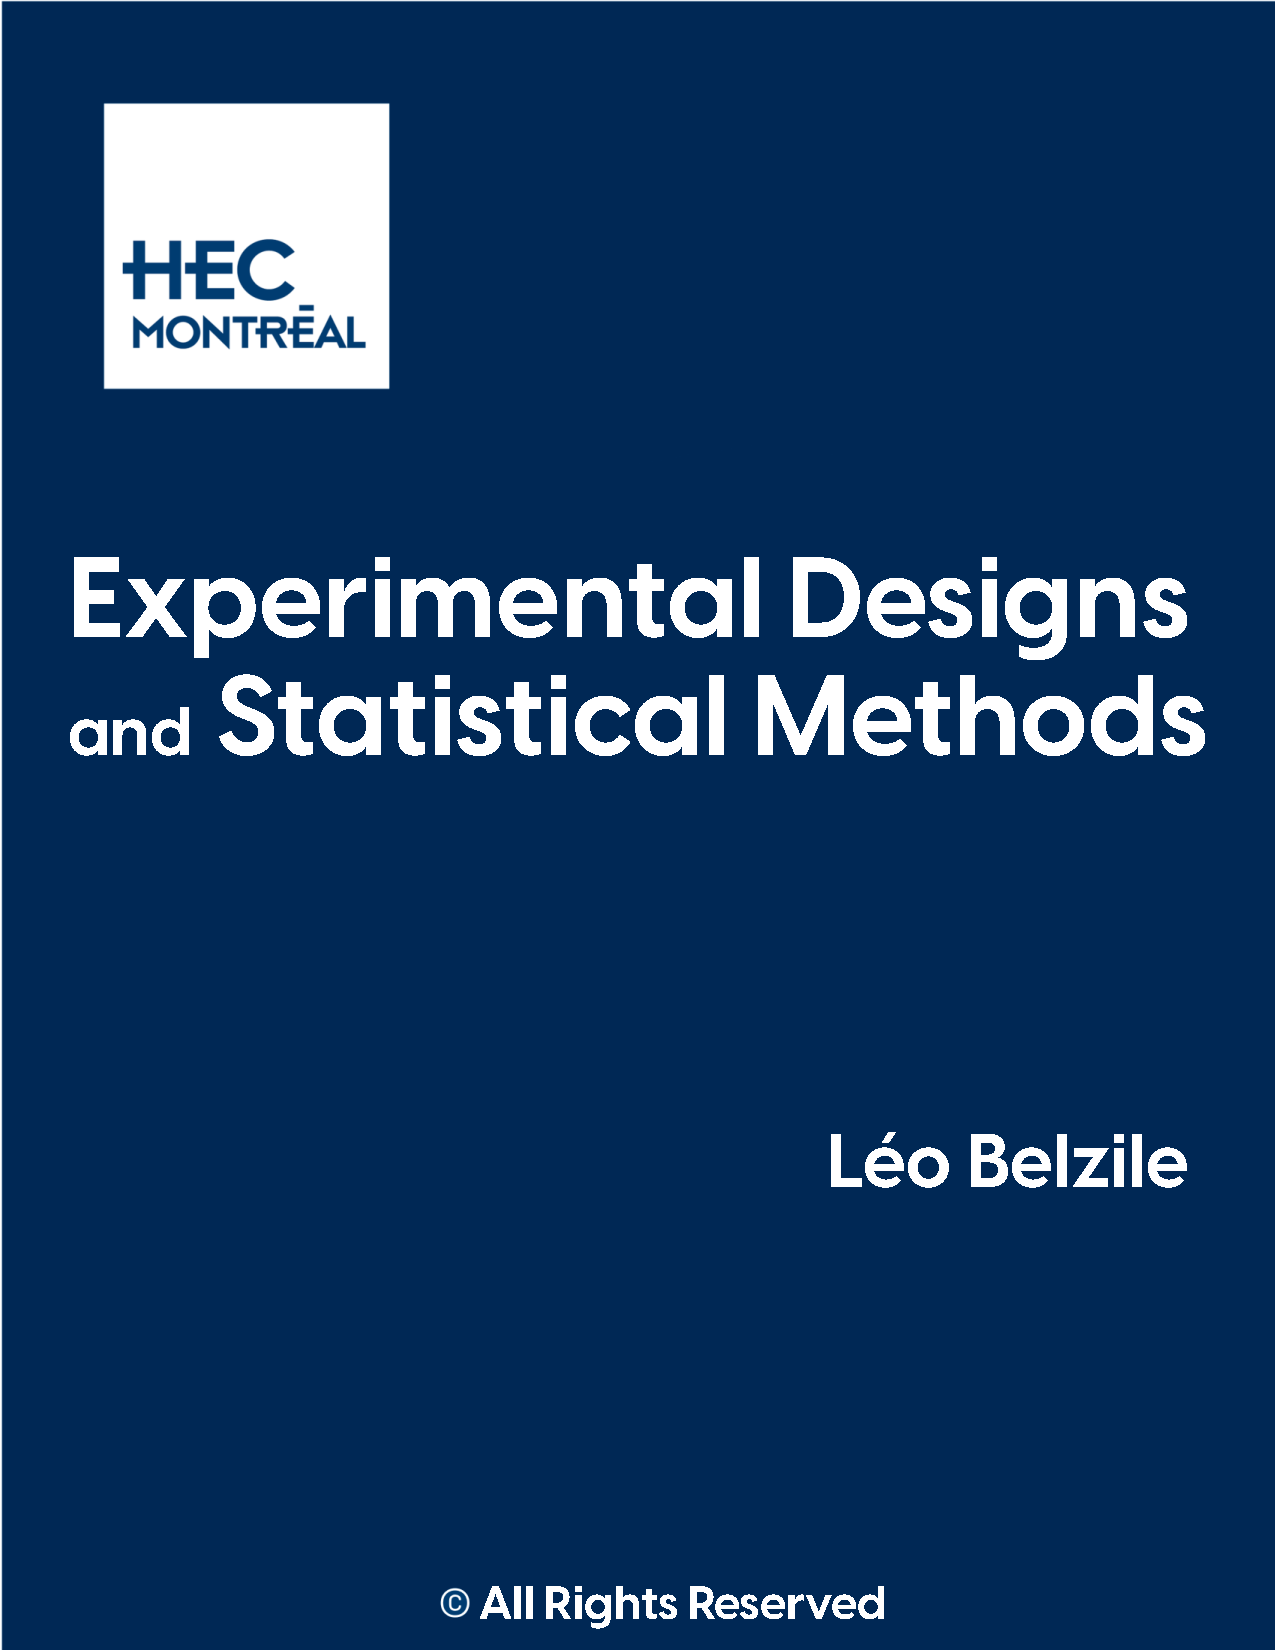
\includepdf{figures/coverpage.pdf}

\ifdefined\Shaded\renewenvironment{Shaded}{\begin{tcolorbox}[interior hidden, borderline west={3pt}{0pt}{shadecolor}, enhanced, sharp corners, breakable, frame hidden, boxrule=0pt]}{\end{tcolorbox}}\fi

\renewcommand*\contentsname{Table of contents}
{
\setcounter{tocdepth}{2}
\tableofcontents
}
\mainmatter
\bookmarksetup{startatroot}

\hypertarget{welcome}{%
\chapter*{Welcome}\label{welcome}}
\addcontentsline{toc}{chapter}{Welcome}

\markboth{Welcome}{Welcome}

This book is a web complement to MATH 80667A \emph{Experimental Designs
and Statistical Methods}, a graduate course offered at HEC Montréal in
the joint Ph.D.~program in Management.

These notes are licensed under a
\href{http://creativecommons.org/licenses/by-nc-sa/4.0/}{Creative
Commons Attribution-NonCommercial-ShareAlike 4.0 International License}
and were last compiled on Sunday, March 24 2024.

The objective of the course is to teach basic principles of experimental
designs and statistical inference using the \textbf{R} programming
language. We will pay particular attention to the correct reporting and
interpretation of results and learn how to review critically scientific
papers using experimental designs. The unifying theme of the book is
that statistics are summary of evidence, and statistic as a field is the
science of decision-making in the presence of uncertainty. We use
examples drawn from published articles in management sciences to
illustrate core concepts.

\bookmarksetup{startatroot}

\hypertarget{introduction}{%
\chapter{Introduction}\label{introduction}}

The advancement of science is built on our ability to study and assess
research hypotheses. This chapter covers the basic concepts of
experiments, starting with vocabulary associated with the field.
Emphasis is placed on the difference between experiments and
observations.

This course covers experimental designs. In an experiment, the
researcher manipulates one or more features (say the complexity of a
text the person must read, or the type of advertisement campaign
displayed, etc.) to study their impact. In general, however (Cox 1958)

\begin{quote}
effects under investigation tend to be masked by fluctuations outside
the experimenter's control.
\end{quote}

The purpose of experiments is to arrange data collection so as to be
capable of disentangling the differences due to treatment from those due
to the (often large) intrinsic variation of the measurements. We
typically expect differences between treatments (and thus the effect) to
be \emph{comparatively stable} relative to the measurement variation.

\begin{tcolorbox}[enhanced jigsaw, colback=white, coltitle=black, rightrule=.15mm, left=2mm, bottomrule=.15mm, toprule=.15mm, titlerule=0mm, colframe=quarto-callout-important-color-frame, leftrule=.75mm, title=\textcolor{quarto-callout-important-color}{\faExclamation}\hspace{0.5em}{\textbf{Learning objectives}:}, breakable, arc=.35mm, colbacktitle=quarto-callout-important-color!10!white, opacitybacktitle=0.6, opacityback=0, toptitle=1mm, bottomtitle=1mm]

\begin{itemize}
\tightlist
\item
  Learning the terminology associated to experiments.
\item
  Assessing the generalizability of a study based on the consideration
  of the sample characteristics, sampling scheme and population.
\item
  Distinguishing between observational and experimental studies.
\item
  Understanding the rationale behind the requirements for good
  experimental studies.
\end{itemize}

\end{tcolorbox}

\hypertarget{study-type}{%
\section{Study type}\label{study-type}}

There are two main categories of studies: observational and
experimental. The main difference between the two is treatment
assignment. In observational studies, a feature or potential cause is
measured, but not assigned by the experimenter. By contrast, the
treatment assignment mechanism is fully determined by the experimenter
in the latter case.

For example, an economist studying the impact of interest rates on the
price of housing can only look at historical records of sales.
Similarly, surveys studying the labour market are also observational:
people cannot influence the type of job performed by employees or their
social benefits to see what could have happened. Observational studies
can lead to detection of association, but only an experiment in which
the researcher controls the allocation mechanism through randomization
can lead to \emph{directly} establish existence of a causal
relationship. Because everything else is the same in a well controlled
experiment, any treatment effect should be in principle caused by the
experimental manipulation.\footnote{The preceding paragraph shouldn't be
  taken to mean that one cannot get meaningful conclusions from
  observational studies. Rather, I wish to highlight that controlling
  for the non-random allocation and potential confounding is a much more
  complicated task, requires practitioners to make stronger (and
  sometimes unverifiable) assumptions and requires using a different
  toolbox (including, but not limited to differences in differences,
  propensity score weighting, instrumental variables). The book
  \href{https://theeffectbook.net/index.html}{\emph{The Effect: An
  Introduction to Research Design and Causality}} by Nick
  Huntington-Klein gives a gentle nontechnical introduction to some of
  these methods.}

\begin{figure}[ht!]

{\centering 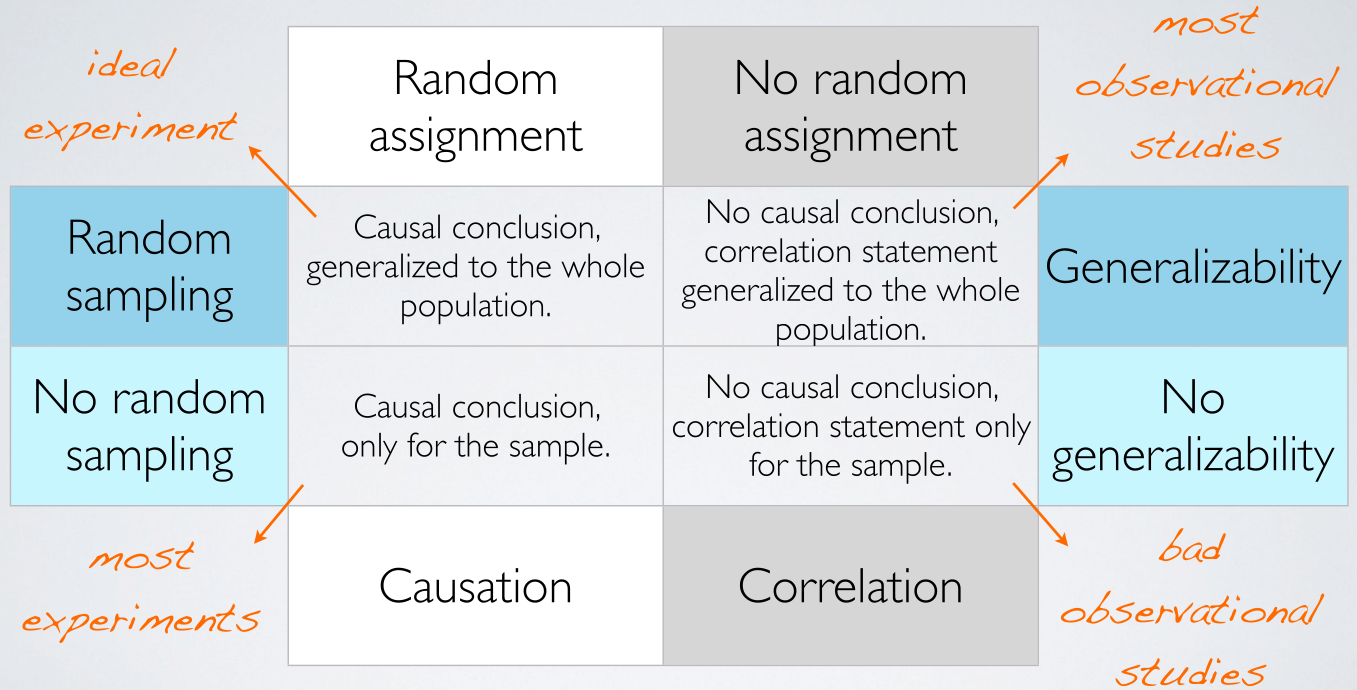
\includegraphics[width=0.8\textwidth,height=\textheight]{figures/random_sample_assignment.png}

}

\caption{\label{fig-openintrograph}Two by two classification matrix for
experiments based on sampling and study type. Source: Mine
Çetinkaya-Rundel and OpenIntro, distributed under the
\href{https://creativecommons.org/licenses/by-sa/3.0/us/}{CC BY-SA
license}.}

\end{figure}

Figure~\ref{fig-openintrograph} summarizes the two preceding sections.
Random allocation of observational units to treatment and random samples
from the population lead to ideal studies, but may be impossible due to
ethical considerations.

\hypertarget{terminology}{%
\section{Terminology}\label{terminology}}

In its simplest form, an \textbf{experimental design} is a comparison of
two or more treatments (experimental conditions):

\begin{itemize}
\tightlist
\item
  The subjects (or \textbf{experimental units}) in the different groups
  of treatment have similar characteristics and are treated exactly the
  same way in the experimentation except for the treatment they are
  receiving. Formally, an experimental unit is the smallest division
  such that any two units may receive different treatments.
\item
  The \textbf{observational unit} is the smallest level (time point,
  individual) at which measurement are recorded.
\item
  Explanatories (independent variables) are variables that impact the
  response. They can be continuous (dose) or categorical variables; in
  the latter case, they are termed \textbf{factors}.
\item
  The \textbf{experimental treatments} or conditions are
  \emph{manipulated and controlled} by the researcher. Oftentimes, there
  is a \textbf{control} or baseline treatment relative to which we
  measure improvement (e.g., a placebo for drugs).
\item
  After the different treatments have been administered to subjects
  participating in a study, the researcher measures one or more outcomes
  (also called responses or dependent variables) on each subject.
\item
  Observed differences in the outcome variable between the experimental
  conditions (treatments) are called treatment effects.
\end{itemize}

\begin{example}[Pedagogical
experience]\protect\hypertarget{exm-experimentdefinitions}{}\label{exm-experimentdefinitions}

Suppose we want to study the effectiveness of different pedagogical
approaches to learning. Evidence-based pedagogical researchs point out
that active learning leads to higher retention of information. To
corroborate this research hypothesis, we can design an experiment in
which different sections of a course are assigned to different teaching
methods. In this example, each student in a class group receives the
same teaching assignment, so the experimental units are the sections and
the observational units are the individual students. The treatment is
the teaching method (traditional teaching versus flipped classroom).

\end{example}

\begin{tcolorbox}[enhanced jigsaw, colback=white, coltitle=black, rightrule=.15mm, left=2mm, bottomrule=.15mm, toprule=.15mm, titlerule=0mm, colframe=quarto-callout-tip-color-frame, leftrule=.75mm, title=\textcolor{quarto-callout-tip-color}{\faLightbulb}\hspace{0.5em}{Your turn}, breakable, arc=.35mm, colbacktitle=quarto-callout-tip-color!10!white, opacitybacktitle=0.6, opacityback=0, toptitle=1mm, bottomtitle=1mm]

The marketing department of a company wants to know the value of its
brand by determining how much more customers are willing to pay for
their product relative to the cheaper generic product offered by the
store. Economic theory suggests a substitution effect: while customers
may prefer the brand product, they will switch to the generic version if
the price tag is too high. To check this theory, one could design an
experiment.

As a researcher, how would you conduct this study? Identify a specific
product. For the latter, define

\begin{itemize}
\tightlist
\item
  an adequate response variable
\item
  the experimental and observational units
\item
  potential blocking factors
\end{itemize}

\end{tcolorbox}

The main reason experiments should be preferred to collection of
observational data is that they allow us, if they are conducted
properly, to draw \textbf{causal conclusions} about the phenomenon of
interest. If we take a random sample from the population of interest,
split it randomly and manipulate only certain aspects, then all
differences between groups must be due to those changes.

As Hariton and Locascio (2018) put it:

\begin{quote}
Randomised controlled trials (RCTs) are the reference standard for
studying causal relationships between interventions and outcomes as
randomisation eliminates much of the bias inherent with other study
designs
\end{quote}

\begin{tcolorbox}[enhanced jigsaw, colback=white, coltitle=black, rightrule=.15mm, left=2mm, bottomrule=.15mm, toprule=.15mm, titlerule=0mm, colframe=quarto-callout-caution-color-frame, leftrule=.75mm, title=\textcolor{quarto-callout-caution-color}{\faFire}\hspace{0.5em}{\textbf{Quasi experiments}}, breakable, arc=.35mm, colbacktitle=quarto-callout-caution-color!10!white, opacitybacktitle=0.6, opacityback=0, toptitle=1mm, bottomtitle=1mm]

Sometimes, it is impossible or unethical to conduct an experiment. This
seemingly precludes study many social phenomena, such as the effect on
women and infantile mortality of strict bans on abortions. When changes
in legislation occur (such as the Supreme court overturning Roe and
Wade), this offers a window to compare neighbouring states.

Canadian economist David Card was co-awarded the 2021 Nobel Memorial
Prize in Economic Sciences for his work in experimental economics. One
of his most cited paper is Card and Krueger (1994), a study that looked
at the impact of an increase in minimum wage on employment figures. Card
and Krueger (1994) used a planned increase of the minimum wage of \$0.80
USD in New Jersey to make comparisons with neighbouring Eastern
Pennsylvania counties by studying 410 fast food outlets. The authors
found no evidence of a negative impact on employment of this hike.

\end{tcolorbox}

\begin{tcolorbox}[enhanced jigsaw, colback=white, coltitle=black, rightrule=.15mm, left=2mm, bottomrule=.15mm, toprule=.15mm, titlerule=0mm, colframe=quarto-callout-important-color-frame, leftrule=.75mm, title=\textcolor{quarto-callout-important-color}{\faExclamation}\hspace{0.5em}{\textbf{Point of terminology: internal and external validity}}, breakable, arc=.35mm, colbacktitle=quarto-callout-important-color!10!white, opacitybacktitle=0.6, opacityback=0, toptitle=1mm, bottomtitle=1mm]

A study from which we can study causal relationships is said to have
\textbf{internal validity}. By design, good experiments should have this
desirable property because the random allocation of treatment
guarantees, if randomization is well performed, that the effect of
interest is causal. There are many other aspects, not covered in the
class, that can threaten internal validity.

\textbf{External validity} refers directly to generalizability of the
conclusions of a study: Figure~\ref{fig-openintrograph} shows that
external validity is directly related to random sampling from the
population

\end{tcolorbox}

\begin{tcolorbox}[enhanced jigsaw, colback=white, coltitle=black, rightrule=.15mm, left=2mm, bottomrule=.15mm, toprule=.15mm, titlerule=0mm, colframe=quarto-callout-important-color-frame, leftrule=.75mm, title=\textcolor{quarto-callout-important-color}{\faExclamation}\hspace{0.5em}{\textbf{Point of terminology: between-subjects and within-subjects
designs}}, breakable, arc=.35mm, colbacktitle=quarto-callout-important-color!10!white, opacitybacktitle=0.6, opacityback=0, toptitle=1mm, bottomtitle=1mm]

In between-subjects designs, subjects are randomly assigned to only one
of the different experimental conditions. On the contrary, participants
receive many or all of the experimental treatments in a within-subjects
design, the order of assignment of the conditions typically being
random.

While within-subject designs allow for a better use of available
ressources (it is cheaper to have fewer participants perform multiple
tasks), observations from within-design are correlated and more subject
to missingness and learning effects, all of which require special
statistical treatment.

\end{tcolorbox}

\hypertarget{review-of-basic-concepts}{%
\section{Review of basic concepts}\label{review-of-basic-concepts}}

\hypertarget{variables}{%
\subsection{Variables}\label{variables}}

The choice of statistical model and test depends on the underlying type
of the data collected. There are many choices: quantitative (discrete or
continuous) if the variables are numeric, or qualitative (binary,
nominal, ordinal) if they can be described using an adjective; I prefer
the term categorical, which is more evocative. The choice of graphical
representation for data is contingent on variable type. Specifically,

\begin{itemize}
\tightlist
\item
  a \textbf{variable} represents a characteristic of the population, for
  example the sex of an individual, the price of an item, etc.
\item
  an \textbf{observation} is a set of measures (variables) collected
  under identical conditions for an individual or at a given time.
\end{itemize}

Most of the models we will deal with are so-called regression models, in
which the mean of a quantitative variable is a function of other
variables, termed explanatories. There are two types of numerical
variables

\begin{itemize}
\tightlist
\item
  a discrete variable takes a countable number of values, prime examples
  being binary variables or count variables.
\item
  a continuous variable can take (in theory) an infinite possible number
  of values, even when measurements are rounded or measured with a
  limited precision (time, width, mass). In many case, we could also
  consider discrete variables as continuous if they take enough values
  (e.g., money).
\end{itemize}

Categorical variables take only a finite of values. They are regrouped
in two groups, nominal if there is no ordering between levels (sex,
colour, country of origin) or ordinal if they are ordered (Likert scale,
salary scale) and this ordering should be reflected in graphs or tables.
We will bundle every categorical variable using arbitrary encoding for
the levels: for modelling, these variables taking \(K\) possible values
(or levels) must be transformed into a set of \(K-1\) binary variables
\(T_1, \ldots, T_K\), each of which corresponds to the logical group
\(k\) (yes = 1, no = 0), the omitted level corresponding to a baseline
when all of the \(K-1\) indicators are zero. Failing to declare
categorical variables in your software is a common mistake, especially
when these are saved in the database using integers (1,2, \(\ldots\))
rather than as text (Monday, Tuesday, \(\ldots\)).

We can characterize the set of all potential values their measurements
can take, together with their frequency, via a \textbf{distribution}.
The latter can be represented graphically using an histogram or a
density plot\footnote{Since continuous data can take any value in the
  interval, we can't talk about the probability of a specific value.
  Rather, the density curve encodes the probability for any given area:
  the higher the curve, the more likely the outcome.} if the data are
continuous, or a bar plot for discrete or categorical measurements.

\begin{example}[Die
toss]\protect\hypertarget{exm-dietoss}{}\label{exm-dietoss}

The distribution of outcomes of a die toss is discrete and takes values
\(1, \ldots, 6\). Each outcome is equally likely with probability
\(1/6\).

\end{example}

\begin{example}[Normal
distribution]\protect\hypertarget{exm-normaldist}{}\label{exm-normaldist}

Mathematical theory suggests that, under general conditions, the
distribution of a sample average is approximately distributed according
to a normal (aka Gaussian) distribution: this result is central to most
of statistics. Normally distributed data are continuous; the
distribution is characterized by a bell curve, light tails and it is
symmetric around it's mean. The shape of the facade of Hallgrímskirkja
church in Reykjavik, shown in Figure~\ref{fig-Hallfrimskirkja}, closely
resembles the density a normal distribution, which lead
\href{https://sites.google.com/view/khoavu-umn/home}{Khoa Vu} to call it
`a normal church' (chuckles).

\begin{figure}[ht!]

{\centering 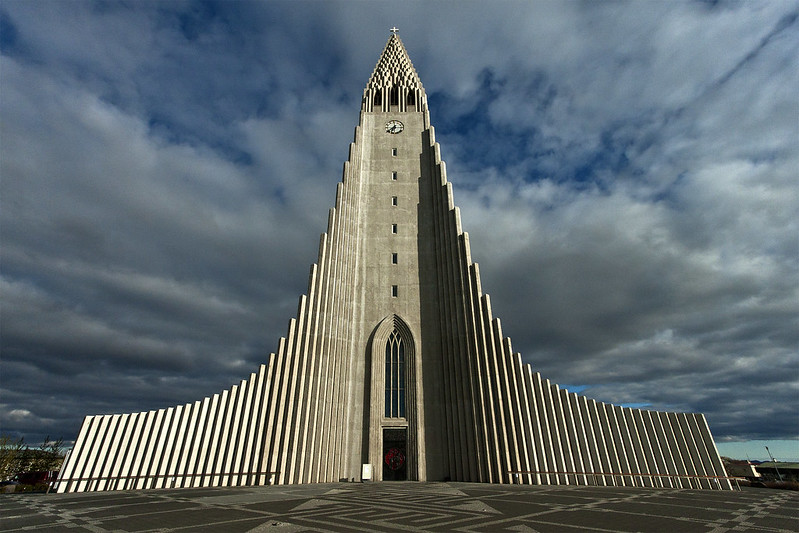
\includegraphics[width=0.8\textwidth,height=\textheight]{figures/hallgrimskirkja_reykjavik.jpg}

}

\caption{\label{fig-Hallfrimskirkja}Photography of the
\href{https://www.flickr.com/photos/dvdhaven/6350588233}{Hallgrímskirkja
church in Reykjavik, Iceland} by Dolf van der Haven, reproduced under a
\href{https://creativecommons.org/licenses/by-nc-nd/2.0/}{CC BY-ND-NC
2.0 license}.}

\end{figure}

The normal distribution is fully characterized by two parameters: the
average \(\mu\) and the standard deviation \(\sigma\). The left panel of
Figure~\ref{fig-normaldist} shows an arbitrary continuous distribution
and the values of a random sample of \(n=1000\) draws. The right panel
shows the histogram of the sample mean value based on a very large
number of random samples of size \(n=25\), drawn from the same
distribution. The superimposed black curve is a normal density curve
whose parameters match those given by the central limit theorem: the
approximation is seemingly quite accurate.

This fact explains the omnipresence of the normal distribution in
introductory data science courses, as well as the prevalence of sample
mean and sample variance as key summary statistics.\footnote{The
  parameters of most commonly used theoretical distributions do not
  directly relate to the mean and the variance, unlike the normal
  distribution.}

\begin{figure}[ht!]

{\centering 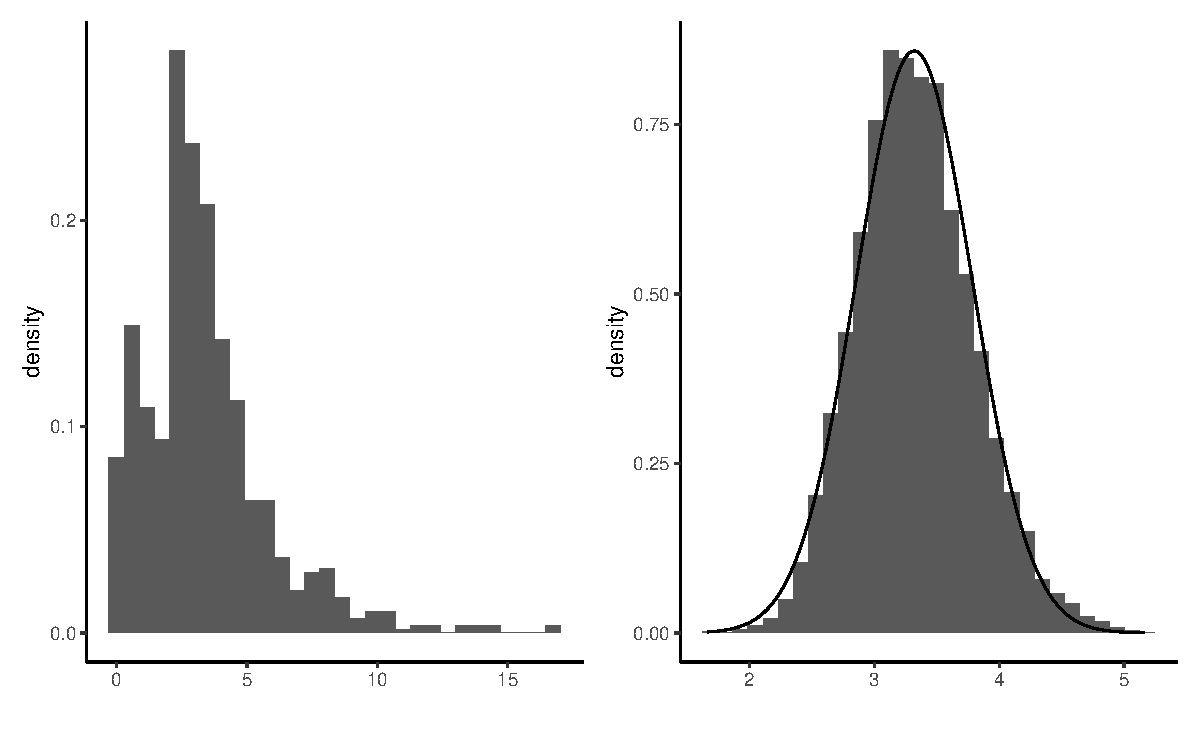
\includegraphics{01-introduction_files/figure-pdf/fig-normaldist-1.pdf}

}

\caption{\label{fig-normaldist}Graphical representation of the
distribution of a continuous variable, with histogram of a sample of
\(n=1000\) observations drawn from the distribution (left) and
distribution of the sample mean, obtained by repeatedly drawing random
sample of \(n=25\) observations and computing their average (right). The
curve shows the normal distribution approximation based on the central
limit theorem.}

\end{figure}

\end{example}

\begin{tcolorbox}[enhanced jigsaw, colback=white, coltitle=black, rightrule=.15mm, left=2mm, bottomrule=.15mm, toprule=.15mm, titlerule=0mm, colframe=quarto-callout-note-color-frame, leftrule=.75mm, title=\textcolor{quarto-callout-note-color}{\faInfo}\hspace{0.5em}{Thinking outside the box}, breakable, arc=.35mm, colbacktitle=quarto-callout-note-color!10!white, opacitybacktitle=0.6, opacityback=0, toptitle=1mm, bottomtitle=1mm]

One key aspect, often neglected in studies, is the discussion of the
metric used for measurement of the response. While previous research may
have identified instruments (like questionnaires) and particular wording
for studying a particular aspect of individuals, there is a lot of free
room for researchers to choose from that may impact conclusions. For
example, if one uses a Likert scale, what should be the range of the
scale? Too coarse a choice may lead to limited capability to detect, but
more truthfulness, while there may be larger intrinsic measurement with
a finer scale.

Likewise, many continuous measures (say fMRI signal) can be discretized
to provide a single numerical value. Choosing the average signal, range,
etc. as outcome variable may lead to different conclusions.

Choosing a particular instrument or metric could be in principle done by
studying (apriori) the distribution of the values for the chosen metric
using a pilot study: this will give researchers some grasp of the
variability of those measures.

\end{tcolorbox}

At the heart of most analysis are measurements. The data presented in
the course have been cleaned and oftentimes the choice of explanatory
variables and experimental factor\footnote{A factor is a categorical
  variable, thus the experimental factor encodes the different groups to
  compare} is evident from the context. In applications, however, this
choice is not always trivial.

\hypertarget{population-sample}{%
\subsection{Population and samples}\label{population-sample}}

Only for well-designed sampling schemes does results generalize beyond
the group observed. It is thus of paramount importance to define the
objective and the population of interest should we want to make
conclusions.

Generally, we will seek to estimate characteristics of a population
using only a sample (a sub-group of the population of smaller size). The
\textbf{population of interest} is a collection of individuals which the
study targets. For example, the Labour Force Survey (LFS) is a monthly
study conducted by Statistics Canada, who define the target population
as ``all members of the selected household who are 15 years old and
older, whether they work or not.'' Asking every Canadian meeting this
definition would be costly and the process would be long: the
characteristic of interest (employment) is also a snapshot in time and
can vary when the person leaves a job, enters the job market or become
unemployed. In this example, collecting a census would be impossible and
too costly.

In general, we therefore consider only \textbf{samples} to gather the
information we seek to obtain. The purpose of \textbf{statistical
inference} is to draw conclusions about the population, but using only a
share of the latter and accounting for sources of variability. The
pollster George Gallup made this great analogy between sample and
population:

\begin{quote}
One spoonful can reflect the taste of the whole pot, if the soup is
well-stirred
\end{quote}

A \textbf{sample} is a sub-group of individuals drawn at random from the
population. We won't focus on data collection, but keep in mind the
following information: for a sample to be good, it must be
representative of the population under study.

\begin{tcolorbox}[enhanced jigsaw, colback=white, coltitle=black, rightrule=.15mm, left=2mm, bottomrule=.15mm, toprule=.15mm, titlerule=0mm, colframe=quarto-callout-tip-color-frame, leftrule=.75mm, title=\textcolor{quarto-callout-tip-color}{\faLightbulb}\hspace{0.5em}{Your turn}, breakable, arc=.35mm, colbacktitle=quarto-callout-tip-color!10!white, opacitybacktitle=0.6, opacityback=0, toptitle=1mm, bottomtitle=1mm]

The
\href{https://www.hec.ca/programmes/baccalaureats/parcours-agir/index.html}{Parcours
AGIR} at HEC Montréal is a pilot project for Bachelor in Administration
students that was initiated to study the impact of flipped classroom and
active learning on performance.

Do you think we can draw conclusions about the efficacy of this teaching
method by comparing the results of the students with those of the rest
of the bachelor program? List potential issues with this approach
addressing the internal and external validity, generalizability, effect
of lurking variables, etc.

\end{tcolorbox}

Because the individuals are selected at \textbf{random} to be part of
the sample, the measurement of the characteristic of interest will also
be random and change from one sample to the next. While larger samples
typically carry more information, sample size is not a guarantee of
quality, as the following example demonstrates.

\begin{example}[Polling for the 1936 USA Presidential
Election]\protect\hypertarget{exm-Galluppoll}{}\label{exm-Galluppoll}

\emph{The Literary Digest} surveyed 10 millions people by mail to know
voting preferences for the 1936 USA Presidential Election. A sizeable
share, 2.4 millions answered, giving Alf Landon (57\%) over incumbent
President Franklin D. Roosevelt (43\%). The latter nevertheless won in a
landslide election with 62\% of votes cast, a 19\% forecast error.
\href{https://www.jstor.org/stable/2749114}{Biased sampling and
differential non-response are mostly responsible for the error:} the
sampling frame was built using ``phone number directories, drivers'
registrations, club memberships, etc.'\,', all of which skewed the
sample towards rich upper class white people more susceptible to vote
for the GOP.

In contrast, Gallup correctly predicted the outcome by polling (only)
50K inhabitants.
\href{https://medium.com/@ozanozbey/how-not-to-sample-11579793dac}{Read
the full story here.}

\end{example}

\begin{tcolorbox}[enhanced jigsaw, colback=white, coltitle=black, rightrule=.15mm, left=2mm, bottomrule=.15mm, toprule=.15mm, titlerule=0mm, colframe=quarto-callout-note-color-frame, leftrule=.75mm, title=\textcolor{quarto-callout-note-color}{\faInfo}\hspace{0.5em}{Thinking outside the box}, breakable, arc=.35mm, colbacktitle=quarto-callout-note-color!10!white, opacitybacktitle=0.6, opacityback=0, toptitle=1mm, bottomtitle=1mm]

What are the considerations that could guide you in determining the
population of interest for your study?

\end{tcolorbox}

\hypertarget{sampling}{%
\subsection{Sampling}\label{sampling}}

Because sampling is costly, we can only collect limited information
about the variable of interest, drawing from the population through a
sampling frame (phone books, population register, etc.) Good sampling
frames can be purchased from sampling firms.

In general, \emph{randomization} is necessary in order to obtain a
\textbf{representative} sample\footnote{Note this randomization is
  different from the one in assigning treatments to experimental units!},
one that match the characteristics of the population. Failing to
randomize leads to introduction of bias and generally the conclusions
drawn from a study won't be generalizable.

Even when observational units are selected at random to participate,
there may be \textbf{bias} introduced due to non-response. In the 1950s,
conducting surveys was relatively easier because most people were listed
in telephone books; nowadays, sampling firms rely on a mix of
interactive voice response and live callers, with sampling frames mixing
landlines, cellphones and online panels together with (heavy) weighting
to correct for non-response. Sampling is a difficult problem with which
we engage only cursorily, but readers are urged to exercise scrutiny
when reading papers.

\begin{tcolorbox}[enhanced jigsaw, colback=white, coltitle=black, rightrule=.15mm, left=2mm, bottomrule=.15mm, toprule=.15mm, titlerule=0mm, colframe=quarto-callout-note-color-frame, leftrule=.75mm, title=\textcolor{quarto-callout-note-color}{\faInfo}\hspace{0.5em}{Thinking outside the box}, breakable, arc=.35mm, colbacktitle=quarto-callout-note-color!10!white, opacitybacktitle=0.6, opacityback=0, toptitle=1mm, bottomtitle=1mm]

Reflect on the choice of platform used to collect answers and think
about how it could influence the composition of the sample returned or
affect non-response in a systematic way.

\end{tcolorbox}

Before examining problems related to sampling, we review the main random
sampling methods. The simplest is simple random sampling, whereby \(n\)
units are drawn completely at random (uniformly) from the \(N\) elements
of the sampling frame. The second most common scheme is stratified
sampling, whereby a certain numbers of units are drawn uniformly from
strata, namely subgroups (e.g., gender). Finally, cluster sampling
consists in sampling only from some of these subgroups.

\begin{example}[Sampling schemes in a
picture]\protect\hypertarget{exm-samplingscheme}{}\label{exm-samplingscheme}

Suppose we wish to look at student satisfaction regarding the material
taught in an introductory statistics course offered to multiple
sections. The population consists of all students enrolled in the course
in a given semester and this list provides the sampling frame. We can
define strata to consist of class group. A simple random sample would be
obtaining by sampling randomly abstracting from class groups, a
stratified sample by drawing randomly a number from each class group and
a cluster sampling by drawing all students from selected class groups.
Cluster sampling is mostly useful if all groups are similar and if the
costs associated to sampling from multiple strata are expensive.

Figure~\ref{fig-sampling} shows three sampling schemes: the middle
corresponds to stratum (e.g., age bands) whereas the right contains
clusters (e.g., villages or classrooms).

\begin{figure}[ht!]

{\centering 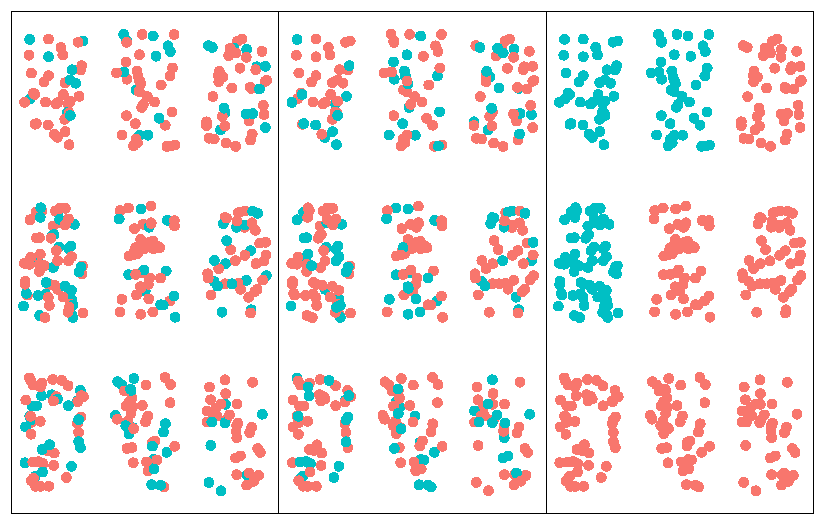
\includegraphics{01-introduction_files/figure-pdf/fig-sampling-1.pdf}

}

\caption{\label{fig-sampling}Illustration of three sampling schemes from
nine groups: simple random sampling (left), stratified sampling (middle)
and cluster sampling (right).}

\end{figure}

Stratified sampling is typically superior if we care about having
similar proportions of sampled in each group and is useful for
reweighting: in Figure~\ref{fig-sampling}, the true proportion of
sampled is \(1/3\), with the simple random sampling having a range of
{[}\(0.22, 0.39\){]} among the strata, compared to {[}\(0.31, 0.33\){]}
for the stratified sample.

\end{example}

\begin{tcolorbox}[enhanced jigsaw, colback=white, coltitle=black, rightrule=.15mm, left=2mm, bottomrule=.15mm, toprule=.15mm, titlerule=0mm, colframe=quarto-callout-note-color-frame, leftrule=.75mm, title=\textcolor{quarto-callout-note-color}{\faInfo}\hspace{0.5em}{Thinking outside the box}, breakable, arc=.35mm, colbacktitle=quarto-callout-note-color!10!white, opacitybacktitle=0.6, opacityback=0, toptitle=1mm, bottomtitle=1mm]

The credibility of a study relies in large part on the quality of the
data collection. Why is it customary to report descriptive statistics of
the sample and a description of the population?

\end{tcolorbox}

There are other instances of sampling, most of which are non-random and
to be avoided whenever possible. These include convenience samples,
consisting of observational units that are easy to access or include
(e.g., friends, students from a university, passerby in the street).
Much like for anecdotal reports, these observational units need not be
representative of the whole population and it is very difficult to
understand how they relate to the latter.

In recent years, there has been a proliferation of studies employing
data obtained from web experimentation plateforms such as Amazon's
Mechanical Turk (MTurk), to the point that the Journal of Management
commissioned a review (Aguinis, Villamor, and Ramani 2021). These
samples are subject to self-selection bias and articles using them
should be read with a healthy dose of skepticism. Unless good
manipulation checks are conducted (e.g., to ensure participants are
faithful and answer in a reasonable amount of time), I would reserve
these tools for paired samples (e.g., asking people to perform multiple
tasks presented in random order) for which the composition of the
population is less important. To make sure your sample matches the
target population, you can use statistical tests and informal comparison
and compare the distribution of individuals with the composition
obtained from the census.

\hypertarget{examples-of-experimental-designs}{%
\section{Examples of experimental
designs}\label{examples-of-experimental-designs}}

The field of experimental design has a long history, starting with
agricultural field trials.

\begin{example}[Agricultural field trials at the Rothamsted Research
Station.]\protect\hypertarget{exm-agriculturalfieldtrials}{}\label{exm-agriculturalfieldtrials}

The \href{https://www.rothamsted.ac.uk/}{Rothamsted Research Station} in
the UK has been conducting experiments since 1843. Ronald A. Fisher, who
worked 14 years at Rothamsted from 1919, developed much of the
statistical theory underlying experimental design, inspired from his
work there. Yates (1964) provides a recollection of his contribution to
the field.

\begin{figure}[ht!]

{\centering 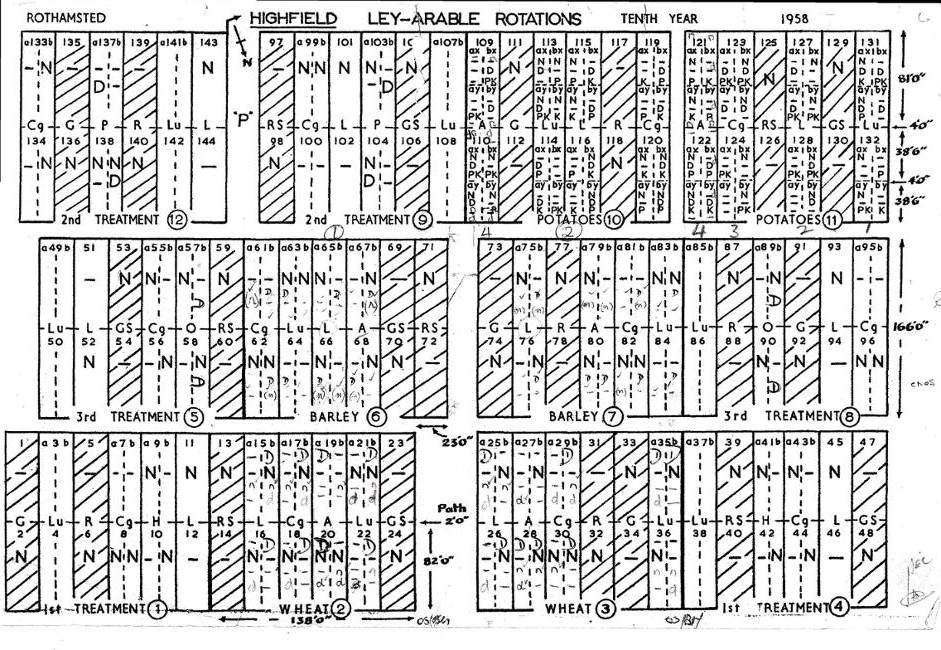
\includegraphics[width=0.8\textwidth,height=\textheight]{figures/HFL-A1958.jpg}

}

\caption{\label{fig-rothamsted}\href{http://www.era.rothamsted.ac.uk/eradoc/article/PS-Highfield-Ley-Arable-1-1}{1958
plan for the Highfield Ley--Arable Experiment}. Source: Rothamsted
Research Station, reproduced under the
\href{https://creativecommons.org/licenses/by/4.0/}{CC BY 4.0 license}.}

\end{figure}

\end{example}

Experimental design revolves in large part in understanding how best to
allocate our resources, determine the impact of policies or choosing the
most effective ``treatment'' from a series of option.

\begin{example}[Modern experiments and A/B
testing]\protect\hypertarget{exm-experimentalexample1}{}\label{exm-experimentalexample1}

Most modern experiments happen online, with tech companies running
thousands of experiments on an ongoing basis in order to discover
improvement to their interfaces that lead to increased profits. An
\href{https://hbr.org/2017/09/the-surprising-power-of-online-experiments}{Harvard
Business Review article} (Kohavi and Thomke 2017) details how small
tweaks to the display of advertisements in the Microsoft Bing search
engine landing page lead to a whooping 12\% increase in revenues. Such
randomized control trials, termed A/B experiments, involve splitting
incoming traffic into separate groups; each group will see different
views of the webpage that differ only ever slightly. The experimenters
then compare traffic and click revenues. At large scale, even small
effects can have major financial consequences and can be learned despite
the large variability in customer behaviour.

\end{example}

There are also multiple examples of randomized control experiments used
for policy making.

\begin{example}[Experiments on wellness
programs]\protect\hypertarget{exm-experimentvsobservations}{}\label{exm-experimentvsobservations}

Song and Baicker (2019) conducted a large randomized trial over a period
of 18 months to study the impact of wellness programs in US companies.
The industry, worth more than 8 billions USD, has significantly
increased following the passage of the Affordable Care Act, aka
Obamacare. The findings are vulgarized in
\href{https://hms.harvard.edu/news/do-wellness-programs-work}{a press
release by Jake Miller from Harvard News \& Research}: they show that,
while there was seemingly an impact on physical activity and well-being,
there were no evidence of changes in absenteeism, job tenure and job
performance. Jones, Molitor, and Reif (2019) reach similar conclusion.

\end{example}

These findings are strikingly different from previous observational
studies, which found increase participation in sportive activities,
increased job duration, reduced medical spendings.

\begin{example}[STAR]\protect\hypertarget{exm-Tennesseestar}{}\label{exm-Tennesseestar}

The Tennessee's Student Teacher Achievement Ratio
\href{(https://dss.princeton.edu/catalog/resource1589)}{(STAR)} project
(Achilles et al. 2008) is another important example of large scale
experiment with broad ramifications. The study suggested that smaller
class sizes lead to better outcomes of pupils.

\begin{quote}
Over 7,000 students in 79 schools were randomly assigned into one of 3
interventions: small class (13 to 17 students per teacher), regular
class (22 to 25 students per teacher), and regular-with-aide class (22
to 25 students with a full-time teacher's aide). Classroom teachers were
also randomly assigned to the classes they would teach. The
interventions were initiated as the students entered school in
kindergarten and continued through third grade.
\end{quote}

\end{example}

\begin{example}[RAND health care
programs]\protect\hypertarget{exm-randcorp}{}\label{exm-randcorp}

In a large-scale
\href{https://www.rand.org/health-care/projects/hie.html}{multiyear
experiment conducted by the RAND Corporation} (Brook et al. 2006),
participants who paid for a share of their health care used fewer health
services than a comparison group given free care. The study concluded
that cost sharing reduced ``inappropriate or unnecessary'' medical care
(overutilization), but also reduced ``appropriate or needed'' medical
care.

\begin{quote}
The HIE was a large-scale, randomized experiment conducted between 1971
and 1982. For the study, RAND recruited 2,750 families encompassing more
than 7,700 individuals, all of whom were under the age of 65. They were
chosen from six sites across the United States to provide a regional and
urban/rural balance. Participants were randomly assigned to one of five
types of health insurance plans created specifically for the experiment.
There were four basic types of fee-for-service plans: One type offered
free care; the other three types involved varying levels of cost sharing
--- 25 percent, 50 percent, or 95 percent coinsurance (the percentage of
medical charges that the consumer must pay). The fifth type of health
insurance plan was a nonprofit, HMO-style group cooperative. Those
assigned to the HMO received their care free of charge. For poorer
families in plans that involved cost sharing, the amount of cost sharing
was income-adjusted to one of three levels: 5, 10, or 15 percent of
income. Out-of-pocket spending was capped at these percentages of income
or at \$1,000 annually (roughly \$3,000 annually if adjusted from 1977
to 2005 levels), whichever was lower.
\end{quote}

\begin{quote}
Families participated in the experiment for 3--5 years. The upper age
limit for adults at the time of enrollment was 61, so that no
participants would become eligible for Medicare before the experiment
ended. To assess participant service use, costs, and quality of care,
RAND served as the families' insurer and processed their claims. To
assess participant health, RAND administered surveys at the beginning
and end of the experiment and also conducted comprehensive physical
exams. Sixty percent of participants were randomly chosen to receive
exams at the beginning of the study, and all received physicals at the
end. The random use of physicals at the beginning was intended to
control for possible health effects that might be stimulated by the
physical exam alone, independent of further participation in the
experiment.
\end{quote}

\end{example}

There are many other great examples in
\href{https://tellingstorieswithdata.com/08-hunt.html\#rct-examples}{the
dedicated section of Chapter 10 of \emph{Telling stories with data} by
Rohan Alexander} (Alexander 2022). Section 1.4 of Berger, Maurer, and
Celli (2018) also lists various applications of experimental designs in
a variety of fields.

\hypertarget{requirements-for-good-experiments}{%
\section{Requirements for good
experiments}\label{requirements-for-good-experiments}}

Section 1.2 of Cox (1958) describes the various requirements that are
necessary for experiments to be useful. These are

\begin{enumerate}
\def\labelenumi{\arabic{enumi}.}
\tightlist
\item
  absence of systematic error
\item
  precision
\item
  range of validity
\item
  simplicity
\end{enumerate}

We review each in turn.

\hypertarget{absence-of-systematic-error}{%
\subsection{Absence of systematic
error}\label{absence-of-systematic-error}}

This point requires careful planning and listing potential confounding
variables that could affect the response.

\begin{example}[Systematic
example]\protect\hypertarget{exm-systematicerror}{}\label{exm-systematicerror}

Suppose we wish to consider the differences in student performance
between two instructors. If the first teaches only morning classes,
while the second only teaches in the evening, it will be impossible to
disentangle the effect of timing with that of instructor performance.
Such comparisons should only be undertaken if there is compelling prior
evidence that timing does not impact the outcome of interest.

\end{example}

The first point raised by Cox is thus that we

\begin{quote}
ensure that experimental units receiving one treatment differ in no
systematic way from those receiving another treatment.
\end{quote}

This point also motivates use of \textbf{double-blind} procedures (where
both experimenters and participants are unaware of the treatment
allocation) and use of placebo in control groups (to avoid psychological
effects, etc. associated with receiving treatment or lack thereof).

Randomization\footnote{The percentage of participants need not be
  equiprobable, nor do we need to assign the same probability to each
  participant. However, going away from equal number of people per group
  has consequences and makes the statistical analysis more complicated.}
is at the core of achieving this goal, and ensuring measurements are
independent of one another also comes out as corollary.

\hypertarget{variability}{%
\subsection{Variability}\label{variability}}

The second point listed by Cox (1958) is that of the variability of
estimator. Much of the precision can be captured by the signal-to-noise
ratio, in which the difference in mean treatment is divided by its
standard error, a form of effect size. The intuition should be that it's
easier to detect something when the signal is large and the background
noise is low. The latter is a function of

\begin{enumerate}
\def\labelenumi{(\alph{enumi})}
\tightlist
\item
  the accuracy of the experimental work and measurements apparatus and
  the intrinsic variability of the phenomenon under study,
\item
  the number of experimental and observational units (the sample size).
\item
  the choice of design and statistical procedures.
\end{enumerate}

Point (a) typically cannot be influenced by the experimenter outside of
choosing the response variable to obtain more reliable measurements.
Point (c) related to the method of analysis, is usually standard unless
there are robustness considerations. Point (b) is at the core of the
planning, notably in choosing the number of units to use and the
allocation of treatment to the different (sub)-units.

\hypertarget{generalizability}{%
\subsection{Generalizability}\label{generalizability}}

Most studies are done with an objective of generalizing the findings
beyond the particular units analyzed. The range of validity thus
crucially depends with the choice of population from which a sample is
drawn and the particular sampling scheme. Non-random sampling severely
limits the extrapolation of the results to more general settings. This
leads Cox to advocate having

\begin{quote}
not just empirical knowledge about what the treatment differences are,
but also some understanding of the reasons for the differences.
\end{quote}

Even if we believe a factor to have no effect, it may be wise to
introduce it in the experiment to check this assumption: if it is not a
source of variability, it shouldn't impact the findings and at the same
time would provide some more robustness.

If we look at a continuous treatment, than it is probably only safe to
draw conclusions within the range of doses administered. Comic in
Figure~\ref{fig-xkcd605} is absurd, but makes this point.

\begin{figure}[ht!]

{\centering 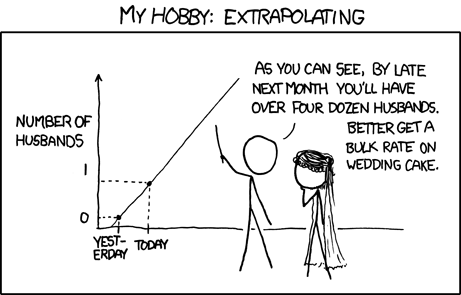
\includegraphics[width=0.5\textwidth,height=\textheight]{figures/xkcd605_extrapolating.png}

}

\caption{\label{fig-xkcd605}xkcd comic \href{https://xkcd.com/605/}{605
(Extrapolating) by Randall Munroe}. Alt text: By the third trimester,
there will be thousands of babies inside you. Cartoon reprinted under
the \href{https://creativecommons.org/licenses/by-nc/2.5/}{CC BY-NC 2.5
license}.}

\end{figure}

\begin{example}[Generalizability]\protect\hypertarget{exm-generalizability}{}\label{exm-generalizability}

Replication studies done in university often draw participants from
students enrolled in the institutions. The findings are thus not
necessarily robust if extrapolated to the whole population if there are
characteristics for which they have strong (familiarity to technology,
acquaintance with administrative system, political views, etc). These
samples are often \textbf{convenience samples}.

\end{example}

\begin{example}[Spratt-Archer barley in
Ireland]\protect\hypertarget{exm-spratt}{}\label{exm-spratt}

Example 1.9 in Cox (1958) mentions recollections of
``Student''\footnote{William Sealy Gosset} on Spratt-Archer barley, a
new variety of barley that performed well in experiments and whose
culture the Irish Department of Agriculture encouraged. Fuelled by a
district skepticism with the new variety, the Department ran an
experiment comparing the yield of the Spratt-Archer barley with that of
the native race. Their findings surprised the experimenters: the native
barley grew more quickly and was more resistant to weeds, leading to
higher yields. It was concluded that the initial experiments were
misleading because Spratt-Archer barley had been experimented in
well-farmed areas, exempt of nuisance.

\end{example}

\hypertarget{simplicity}{%
\subsection{Simplicity}\label{simplicity}}

The fourth requirement is one of simplicity of design, which almost
invariably leads to simplicity of the statistical analysis. Randomized
control-trials are often viewed as the golden rule for determining
efficacy of policies or treatments because the set of assumptions they
make is pretty minimalist due to randomization. Most researchers in
management are not necessarily comfortable with advanced statistical
techniques and this also minimizes the burden. Figure~\ref{fig-xkcd2400}
shows an
\href{https://www.zq1.de/~bernhard/images/share/mRNA-1273-trial.png}{hypothetical
graph} on the efficacy of the Moderna MRNA vaccine for Covid: if the
difference is clearly visible in a suitable experimental setting, then
conclusions are easily drawn.

Randomization justifies the use of the statistical tools we will use
under very weak assumptions, if units measurements are independent from
one another. Drawing conclusions from observational studies, in contrast
to experimental designs, requires making often unrealistic or
unverifiable assumptions and the choice of techniques required to handle
the lack of randomness is often beyond the toolbox of applied
researchers.

\begin{figure}[ht!]

{\centering 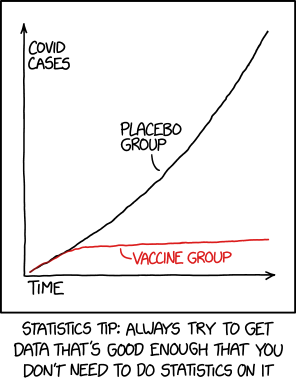
\includegraphics[width=0.4\textwidth,height=\textheight]{figures/xkcd2400_statistics.png}

}

\caption{\label{fig-xkcd2400}xkcd comic
\href{https://xkcd.com/2400/}{2400 (Statistics) by Randall Munroe}. Alt
text: We reject the null hypothesis based on the `hot damn, check out
this chart' test. Cartoon reprinted under the
\href{https://creativecommons.org/licenses/by-nc/2.5/}{CC BY-NC 2.5
license}.}

\end{figure}

\begin{tcolorbox}[enhanced jigsaw, colback=white, coltitle=black, rightrule=.15mm, left=2mm, bottomrule=.15mm, toprule=.15mm, titlerule=0mm, colframe=quarto-callout-tip-color-frame, leftrule=.75mm, title=\textcolor{quarto-callout-tip-color}{\faLightbulb}\hspace{0.5em}{Your turn}, breakable, arc=.35mm, colbacktitle=quarto-callout-tip-color!10!white, opacitybacktitle=0.6, opacityback=0, toptitle=1mm, bottomtitle=1mm]

\begin{itemize}
\tightlist
\item
  Define the following terms in your own word: experimental unit,
  factor, treatment.
\item
  What is the main benefit of experimental studies over observational
  studies?
\end{itemize}

\end{tcolorbox}

\bookmarksetup{startatroot}

\hypertarget{hypothesis-testing}{%
\chapter{Hypothesis testing}\label{hypothesis-testing}}

In most applied domains, empirical evidences drive the advancement of
the field and data from well designed experiments contribute to the
built up of science. In order to draw conclusions in favour or against a
theory, researchers turn (often unwillingly) to statistics to back up
their claims. This has led to the prevalence of the use of the null
hypothesis statistical testing (NHST) framework. One important aspect of
the reproducibility crisis is the misuse of \(p\)-values in journal
articles: falsification of a null hypothesis is not enough to provide
substantive findings for a theory.

Because introductory statistics course typically present hypothesis
tests without giving much thoughts to the underlying construction
principles of such procedures, users often have a reductive view of
statistics as a catalogue of pre-determined procedures. To make a
culinary analogy, users focus on learning recipes rather than trying to
understand the basics of cookery. This chapter focuses on understanding
of key ideas related to testing.

\begin{tcolorbox}[enhanced jigsaw, colback=white, coltitle=black, rightrule=.15mm, left=2mm, bottomrule=.15mm, toprule=.15mm, titlerule=0mm, colframe=quarto-callout-important-color-frame, leftrule=.75mm, title=\textcolor{quarto-callout-important-color}{\faExclamation}\hspace{0.5em}{Key concept}, breakable, arc=.35mm, colbacktitle=quarto-callout-important-color!10!white, opacitybacktitle=0.6, opacityback=0, toptitle=1mm, bottomtitle=1mm]

\textbf{Learning objectives}:

\begin{itemize}
\tightlist
\item
  Understanding the role of uncertainty in decision making.
\item
  Understanding the importance of signal-to-noise ratio as a measure of
  evidence.
\item
  Knowing the basic ingredients of hypothesis testing and being capable
  of correctly formulating and identifying these components in a paper.
\item
  Correctly interpreting \(p\)-values and confidence intervals for a
  parameter.
\end{itemize}

\end{tcolorbox}

\hypertarget{hypothesis}{%
\section{Hypothesis}\label{hypothesis}}

The first step of a design is formulating a research question.
Generally, this hypothesis will specify potential differences between
population characteristics due to some intervention (a treatment) that
the researcher wants to quantify. This is the step during which
researchers decide on sample size, choice of response variable and
metric for the measurement, write down the study plan, etc.

It is important to note that most research questions cannot be answered
by simple tools. Researchers wishing to perform innovative
methodological research should contact experts and consult with
statisticians \textbf{before} they collect their data to get information
on how best to proceed for what they have in mind so as to avoid the
risk of making misleading and false claims based on incorrect analysis
or data collection.

\begin{figure}[ht!]

{\centering 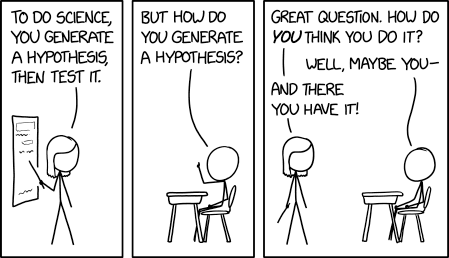
\includegraphics[width=0.6\textwidth,height=\textheight]{figures/xkcd2569_hypothesis_generation.png}

}

\caption{\label{fig-xkcd2569}xkcd comic
\href{https://xkcd.com/2569/}{2569 (Hypothesis generation) by Randall
Munroe}. Alt text: Frazzled scientists are requesting that everyone
please stop generating hypotheses for a little bit while they work
through the backlog. Cartoon reprinted under the
\href{https://creativecommons.org/licenses/by-nc/2.5/}{CC BY-NC 2.5
license}.}

\end{figure}

\hypertarget{sampling-variability}{%
\section{Sampling variability}\label{sampling-variability}}

Given data, a researcher will be interested in estimating particular
characteristics of the population. We can characterize the set of all
potential values their measurements can take, together with their
frequency, via a distribution.

The purpose of this section is to illustrate how we cannot simply use
raw differences between groups to make meaningful comparisons: due to
sampling variability, samples will be alike even if they are generated
in the same way, but there will be always be differences between their
summary statistics. Such differences tend to attenuate (or increase) as
we collect more sample. Inherent to this is the fact that as we gather
more data (and thus more information) about our target, the portrait
becomes more precise. This is ultimately what allows us to draw
meaningful conclusions but, in order to do so, we need first to
determine what is likely or plausible and could be a stroke of luck, and
what is not likely to occur solely due to randomness.

\begin{example}[A/B
testing]\protect\hypertarget{exm-ABtest}{}\label{exm-ABtest}

Consider two webpage design: one is the current version (\emph{status
quo}) and the other implementation contains a clickable banner in a
location where eyetracker suggest that viewers eyes spend more time or
attention. The number of clicks on those headlines are what generate
longer viewing, and thus higher revenues from advertisement. The
characteristic of interest here would be the average click conversation
rate for each of the webpage design.

It is fairly simple to redirect traffic so that a random fraction gets
assigned to the new design for study. After a suitable period of time,
the data can be analyzed to see if the new webpage generates more
clicks.

\end{example}

An hypothesis test will focus on one or multiple of these
characteristics. Suppose for simplicity that we have only two groups,
control and treatment, whose population averages are \(\mu_C\) and
\(\mu_T\) we wish to compare. People commonly look at the difference in
average, say \(\delta=\mu_T - \mu_C\) as a measure of the effectiveness
of the treatment.\footnote{We could look at the ratio \(\mu_T/\mu_C\)
  instead.} If we properly randomized observations in each subgroup and
nothing else changes, then this measures the impact of the treatment.
Because we only have a sample at hand and not the whole population, we
don't know for sure the values of \(\mu_C\) and \(\mu_T\). These
quantities exist, but are unknown to us so the best we can do is
estimate them using our sample. If we have a random sample from the
population, then the characteristics of the sample will be (noisy)
proxys of those of the population.

We call numerical summaries of the data \textbf{statistics}. Its
important to distinguish between procedures/formulas and their numerical
values. An \textbf{estimator} is a rule or formula used to calculate an
estimate of some parameter or quantity of interest based on observed
data (like a recipe for cake). Once we have observed data we can
actually compute the sample mean, that is, we have an estimate --- an
actual value (the cake), which is a single realization and not random.
In other words,

\begin{itemize}
\tightlist
\item
  an estimand is our conceptual target, like the population
  characteristic of interest (population mean).
\item
  an estimator is the procedure or formula telling us how to transform
  the sample data into a numerical summary that is a proxy of our
  target.
\item
  an estimate is a number, the numerical value obtained once we apply
  the formula to observed data.
\end{itemize}

\begin{figure}

\begin{minipage}[t]{0.33\linewidth}

{\centering 

\raisebox{-\height}{

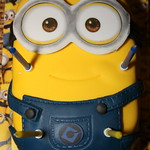
\includegraphics{figures/estimand.jpg}

}

}

\subcaption{\label{fig-cake-1}Estimand}
\end{minipage}%
%
\begin{minipage}[t]{0.33\linewidth}

{\centering 

\raisebox{-\height}{

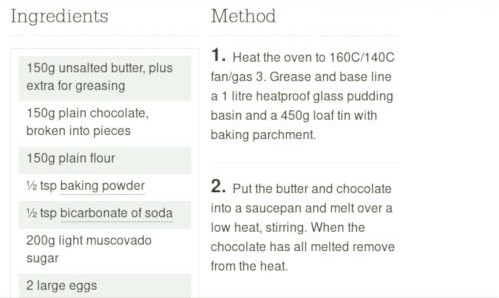
\includegraphics{figures/estimator.jpg}

}

}

\subcaption{\label{fig-cake-2}Estimator}
\end{minipage}%
%
\begin{minipage}[t]{0.33\linewidth}

{\centering 

\raisebox{-\height}{

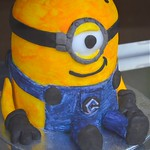
\includegraphics{figures/estimate.jpg}

}

}

\subcaption{\label{fig-cake-3}Estimate}
\end{minipage}%

\caption{\label{fig-cake}\href{https://www.flickr.com/photos/darkdwarf/16563489881}{Estimand}
(left), estimator (middle) and
\href{https://www.flickr.com/photos/bensutherland/14685548773}{estimate}
(right) illustrated with cakes and based on an original idea of Simon
Grund. Cake photos shared under
\href{https://creativecommons.org/licenses/by-nc/2.0/}{CC BY-NC 2.0
license}.}

\end{figure}

For example, we may use as estimand the population average of
\(Y_1, \ldots\), say \(\mu\). The estimator will be sample mean, i.e.,
the sum of the elements in the sample divided by the sample size,
\(\overline{Y}=(Y_1 + \cdots + Y_n)/n\). The estimate will be a
numerical value, say 4.3.

Because the inputs of the estimator are random, the output is also
random and change from one sample to the next: even if you repeat a
recipe, you won't get the exact same result every time, as in
Figure~\ref{fig-xkcd605}.

\begin{figure}[ht!]

{\centering 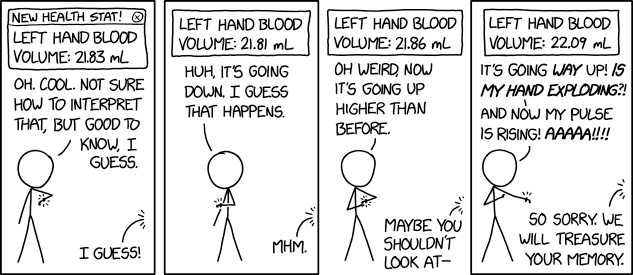
\includegraphics[width=0.7\textwidth,height=\textheight]{figures/xkcd2581_health_stats.png}

}

\caption{\label{fig-xkcd605}xkcd comic
\href{https://xkcd.com/2581/}{2581 (Health Stats) by Randall Munroe}.
Alt text: You will live on forever in our hearts, pushing a little extra
blood toward our left hands now and then to give them a squeeze. Cartoon
reprinted under the
\href{https://creativecommons.org/licenses/by-nc/2.5/}{CC BY-NC 2.5
license}.}

\end{figure}

To illustrate this point, Figure~\ref{fig-samplevar} shows five simple
random samples of size \(n=10\) drawn from an hypothetical population
with mean \(\mu\) and standard deviation \(\sigma\), along with their
sample mean \(\overline{y}\). Thus, sampling variability implies that
the sample means of the subgroups will always differ even if they share
the same characteristics. You can view sampling variability as noise:
our goal is to extract the signal (typically differences in means) but
accounting for spurious results due to the background noise.

\begin{figure}[ht!]

{\centering 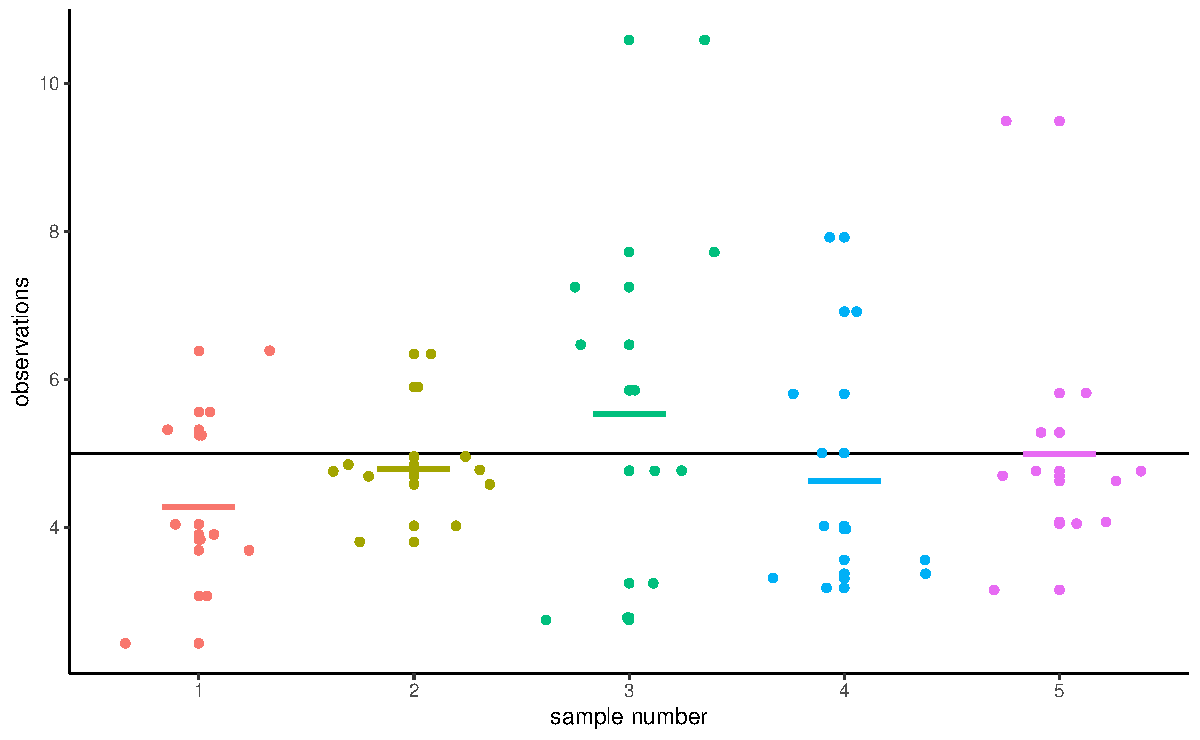
\includegraphics{02-hypothesis_testing_files/figure-pdf/fig-samplevar-1.pdf}

}

\caption{\label{fig-samplevar}Five samples of size \(n=10\) drawn from a
common population with mean \(\mu\) (horizontal line). The colored
segments show the sample means of each sample.}

\end{figure}

We can clearly see from Figure~\ref{fig-samplevar} that, even if each
sample is drawn from the same population, the sample mean varies from
one sample to the next as a result of the sampling variability. The
astute eye might even notice that the sample means are less dispersed
around the full black horizontal line representing the population
average \(\mu\) than are the individual measurements. This is a
fundamental principle of statistics: information accumulates as you get
more data.

Values of the sample mean don't tell the whole picture and studying
differences in mean (between groups, or relative to a postulated
reference value) is not enough to draw conclusions. In most settings,
there is no guarantee that the sample mean will be equal to it's true
value because it changes from one sample to the next: the only guarantee
we have is that it will be on average equal to the population average in
repeated samples. Depending on the choice of measurement and variability
in the population, there may be considerable differences from one
observation to the next and this means the observed difference could be
a fluke.

To get an idea of how certain something is, we have to consider the
variability of an observation \(Y_i\). This variance of an observation
drawn from the population is typically denoted \(\sigma^2\) and it's
square root, the standard deviation, by \(\sigma\).

The sample variance \(S_n\) is an estimator of the standard deviation
\(\sigma\), where \begin{align*}
S^2_n &= \frac{1}{n-1} \sum_{i=1}^n (Y_i-\overline{Y})^2
\end{align*} is the sum of squared difference between observations and
the sample average, scaled by a factor proportional to the sample size.

The standard deviation \emph{of a statistic} is termed \textbf{standard
error}; it should not be confused with the standard deviation \(\sigma\)
of the population from which the sample observations
\(Y_1, \ldots, Y_n\) are drawn. Both standard deviation and standard
error are expressed in the same units as the measurements, so are easier
to interpret than variance. Since the standard error is a function of
the sample size, it is however good practice to report the estimated
standard deviation in reports.

\begin{example}[Sample proportion and uniform
draws]\protect\hypertarget{exm-samppropunif}{}\label{exm-samppropunif}

To illustrate the concept of sampling variability, we follow the lead of
\href{https://www.crumplab.com/statistics/foundations-for-inference.html}{Matthew
Crump} and consider samples from a uniform distribution on
\(\{1, 2, \ldots, 10\}\) each number in this interval is equally likely
to be sampled.

\begin{figure}[ht!]

{\centering 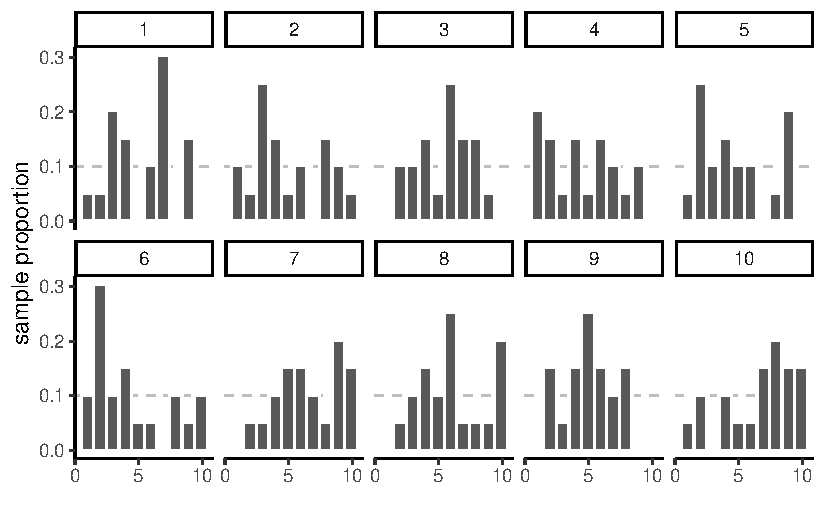
\includegraphics{02-hypothesis_testing_files/figure-pdf/fig-unifsamp1-1.pdf}

}

\caption{\label{fig-unifsamp1}Histograms for 10 random samples of size
\(n=20\) from a discrete uniform distribution.}

\end{figure}

Even if they are drawn from the same population, the 10 samples in
Figure~\ref{fig-unifsamp1} look quite different. The only thing at play
here is the sample variability: since there are \(n=20\) observations in
total, there should be on average 10\% of the observations in each of
the 10 bins, but some bins are empty and others have more counts than
expected. This fluctuation is due to randomness, or chance.

How can we thus detect whether what we see is compatible with the model
we think generated the data? The key is to collect more observations:
the bar height is the sample proportion, an average of 0/1 values with
ones indicating that the observation is in the bin and zero otherwise.

Consider now what happens as we increase the sample size: the top panel
of Figure~\ref{fig-uniformsamp2} shows uniform samples for increasing
samples size. The histogram looks more and more like the true underlying
distribution (flat, each bin with equal frequency) as the sample size
increases. The sample distribution of points is nearly indistinguishable
from the theoretical one (straight line) when \(n=10 000\).\footnote{The
  formula shows that the standard error decreases by a tenfold every
  time the sample size increases by a factor 100.} The bottom panel, on
the other hand, isn't from a uniform distribution and larger samples
come closer to the population distribution. We couldn't have spotted
this difference in the first two plots, since the sampling variability
is too important; there, the lack of data in some bins could have been
attributed to chance, as they are comparable with the graph for data
that are truly uniform. This is in line with most practical
applications, in which the limited sample size restricts our capacity to
disentangle real differences from sampling variability. We must embrace
this uncertainty: in the next section, we outline how hypothesis testing
helps us disentangle the signal from the noise.

\begin{figure}[ht!]

{\centering 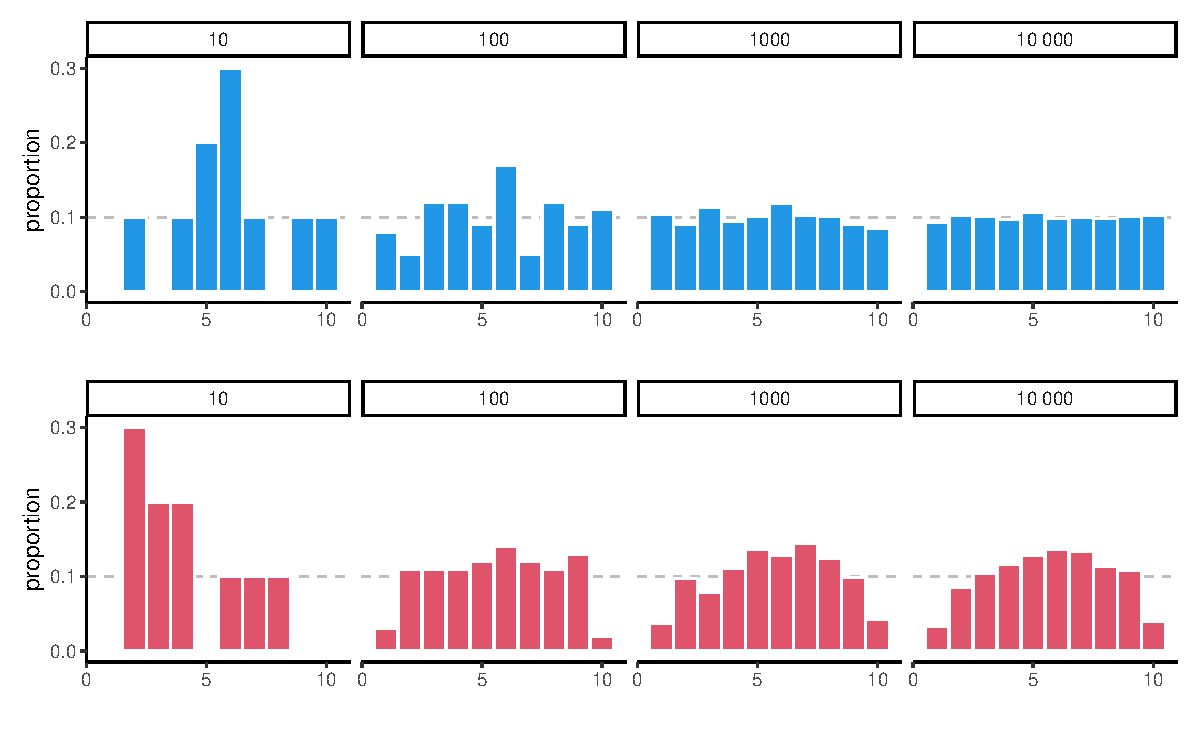
\includegraphics{02-hypothesis_testing_files/figure-pdf/fig-uniformsamp2-1.pdf}

}

\caption{\label{fig-uniformsamp2}Histograms of data from a uniform
distribution (top) and non-uniform (bottom) with increasing sample sizes
of 10, 100, 1000 and 10 000 (from left to right).}

\end{figure}

\end{example}

\hypertarget{tests}{%
\section{Hypothesis testing}\label{tests}}

An hypothesis test is a binary decision rule (yes/no) used to evaluate
the statistical evidence provided by a sample to make a decision
regarding the underlying population. The main steps involved are:

\begin{itemize}
\tightlist
\item
  define the model parameters
\item
  formulate the alternative and null hypothesis
\item
  choose and calculate the test statistic
\item
  obtain the null distribution describing the behaviour of the test
  statistic under \(\mathscr{H}_0\)
\item
  calculate the \emph{p}-value
\item
  conclude (reject or fail to reject \(\mathscr{H}_0\)) in the context
  of the problem.
\end{itemize}

A good analogy for hypothesis tests is a trial for murder on which you
are appointed juror.

\begin{itemize}
\tightlist
\item
  The judge lets you choose between two mutually exclusive outcome,
  guilty or not guilty, based on the evidence presented in court.
\item
  The presumption of innocence applies and evidences are judged under
  this optic: are evidence remotely plausible if the person was
  innocent? The burden of the proof lies with the prosecution to avoid
  as much as possible judicial errors. The null hypothesis
  \(\mathscr{H}_0\) is \emph{not guilty}, whereas the alternative
  \(\mathscr{H}_a\) is \emph{guilty}. If there is a reasonable doubt,
  the verdict of the trial will be not guilty.
\item
  The test statistic (and the choice of test) represents the summary of
  the proof. The more overwhelming the evidence, the higher the chance
  the accused will be declared guilty. The prosecutor chooses the proof
  so as to best outline this: the choice of evidence (statistic)
  ultimately will maximize the evidence, which parallels the power of
  the test.
\item
  The null distribution is the benchmark against which to judge the
  evidence (jurisprudence). Given the proof, what are the odds assuming
  the person is innocent? Since this is possibly different for every
  test, it is common to report instead a \emph{p}-value, which gives the
  level of evidence on a uniform scale which is most easily interpreted.
\item
  The final step is the verdict, a binary decision with outcomes: guilty
  or not guilty. For an hypothesis test performed at level \(\alpha\),
  one would reject (guilty) if the \emph{p}-value is less than
  \(\alpha\). Even if we declare the person not guilty, this doesn't
  mean the defendant is innocent and vice-versa.
\end{itemize}

\hypertarget{hypothesis-1}{%
\subsection{Hypothesis}\label{hypothesis-1}}

In statistical tests we have two hypotheses: the null hypothesis
(\(\mathscr{H}_0\)) and the alternative hypothesis (\(\mathscr{H}_a\)).
Usually, the null hypothesis (the `status quo') is a single numerical
value. The alternative is what we're really interested in testing. In
Figure~\ref{fig-samplevar}, we could consider whether all five groups
have the same mean \(\mathscr{H}_0: \mu_1 = \mu_2 = \cdots = \mu_5\)
against the alternative that at least two of them are different. These
two outcomes are mutually exclusive and cover all possible scenarios. A
statistical hypothesis test allows us to decide whether or not our data
provides enough evidence to reject \(\mathscr{H}_0\) in favor of
\(\mathscr{H}_a\), subject to some pre-specified risk of error: while we
know that the differences are just due to sampling variability in
Figure~\ref{fig-samplevar} because the data is simulated, in practice we
need to assess the evidence using a numerical summary.

\begin{example}[A/B testing
(continued)]\protect\hypertarget{exm-abtest-cont}{}\label{exm-abtest-cont}

We follow-up with our A/B test experiment. Given \(\mu_1\) the
population average click conversation rate for the current webpage and
\(\mu_2\), that of the redesign, we are interested in the
\emph{one-sided hypothesis} that \(\mathscr{H}_0: \mu_2 \leq \mu_1\)
against the alternative (that we are trying to prove)
\(\mathscr{H}_a: \mu_2 > \mu_1\). In choosing as null hypothesis that
the new design is no better or worst, we are putting all our weight to
make sure the changes carry forward if there is overwhelming evidence
that the new design is better and allow us to generate more revenues,
given the costs associated to changes to the interface and the resulting
disruption.

One-sided hypothesis are directional: we care only about a specific
direction, and so here \(\mathscr{H}_a: \mu_2 > \mu_1\). Indeed, if the
experiment suggests that the conversion rate is worst with the new
webpage design, we won't go forward.

Since neither of these population averages \(\mu_1\) and \(\mu_2\) are
known to us, we can work instead with
\(\mathscr{H}_0: \mu_2-\mu_1 \geq 0\). We can use as estimator for the
difference \(\mu_2-\mu_1\) the difference in sample average in each
subgroup.

The null hypothesis here is an interval, but it suffices the consider
the most beneficial scenario, which is \(\mu_2-\mu_1=0\). Indeed, if we
can disprove that there is no difference and see an increase of the
click rate with the updated version, all more extreme cases are
automatically discarded in favour of the alternative that the new design
is better.

One-sided tests for which the evidence runs contrary to the hypothesis
(say the mean conversion rate is higher for the current design than for
the new one) lead to \emph{p}-values of 1, since there is no proof
against the null hypothesis that the old design (the status quo) is
better.

\end{example}

The previous example illustrates the fact that, when writing down null
and alternative hypotheses, what we are trying to prove is typically the
alternative.

In pairwise comparisons or contrasts, we can assign a directionality.
The benefit is that, if we are sure of the direction of the postulated
effect, we only consider as extreme scenarios that run in the direction
we postulated\footnote{This implies that the level \(\alpha\) is all on
  one side, rather than split equally between both tails of the
  distribution. In practice, this translates into increased power of
  detection provided the effect is in the postulated direction.}
However, if the empirical evidence runs contrary to our guess, then
there is no support for the hypothesis.

In more general statistical models, it helps to view the null hypothesis
as a simplification of a more complex model: the latter will fit the
data better because it is more flexible, but we would fail to reject the
null unless this improvement is drastic. For example, in an analysis of
variance model, we compare different mean in each of \(K\) groups
against a single common average.

\hypertarget{test-statistic}{%
\subsection{Test statistic}\label{test-statistic}}

A test statistic \(T\) is a function of the data which takes the data as
input and outputs a summary of the information contained in the sample
for a characteristic of interest, say the population mean. In order to
assess whether the numerical value for \(T\) is unusual, we need to know
what are the potential values taken by \(T\) and their relative
probability if \(\mathscr{H}_0\) is true. We need to know what values we
should expect if, e.g., there was no difference in the averages of the
different groups: this requires a benchmark.

Many statistics we will consider are of the form\footnote{This class of
  statistic, which includes \(t\)-tests, are called Wald statistics.}
\begin{align*}
T = \frac{\text{estimated effect}- \text{postulated effect}}{\text{estimated effect variability}} = \frac{\widehat{\theta} - \theta_0}{\mathrm{se}(\widehat{\theta})}
\end{align*} where \(\widehat{\theta}\) is an estimator of \(\theta\),
\(\theta_0\) is the postulated value of the parameter and
\(\mathrm{se}(\widehat{\theta})\) is the standard error of the test
statistic \(\widehat{\theta}\). This quantity is designed so that, if
our postulated value \(\theta_0\) is correct, \(T\) has approximately
mean zero and variance one. This standardization makes comparison
easier; in fact, the form of the test statistic is chosen so that it
doesn't depend on the measurement units.

For example, if we are interested in mean differences between treatment
group and control group, denoted \(\mu_T\) and \(\mu_C\), then
\(\theta = \mu_T-\mu_C\) and \(\mathscr{H}_0: \mu_T = \mu_C\)
corresponds to \(\mathscr{H}_0: \theta = 0\) for no difference. The
two-sample \(t\)-test would have numerator
\(\widehat{\theta} = \overline{Y}_T - \overline{Y}_C\), where
\(\overline{Y}_T\) is the sample average in treatment group and
\(\overline{Y}_C\) that of the control group. The postulated value for
the mean difference is zero.

The numerator would thus consist of the difference in sample means and
the denominator the standard error of that quantity, calculated using a
software.\footnote{Assuming equal variance, the denominator is estimated
  using the pooled variance estimator.}

\hypertarget{null-distribution-and-p-value}{%
\subsection{\texorpdfstring{Null distribution and
\emph{p}-value}{Null distribution and p-value}}\label{null-distribution-and-p-value}}

The \emph{p}-value allows us to decide whether the observed value of the
test statistic \(T\) is plausible under \(\mathscr{H}_0\). Specifically,
the \emph{p}-value is the probability that the test statistic is equal
or more extreme to the estimate computed from the data, assuming
\(\mathscr{H}_0\) is true. Suppose that based on a random sample
\(Y_1, \ldots, Y_n\) we obtain a statistic whose value \(T=t\). For a
two-sided test \(\mathscr{H}_0:\theta=\theta_0\)
vs.~\(\mathscr{H}_a:\theta \neq \theta_0\), the \emph{p}-value is
\(\mathsf{Pr}_0(|T| \geq |t|)\).\footnote{If the distribution of \(T\)
  is symmetric around zero, the \emph{p}-value reduces to
  \(p = 2 \times \mathsf{Pr}_0(T \geq |t|).\)}

How do we determine the null distribution given that the true data
generating mechanism is unknown to us? We ask a statistician! In simple
cases, it might be possible to enumerate all possible outcomes and thus
quantity the degree of outlyingness of our observed statistic. In more
general settings, we can resort to simulations or to probability theory:
the central limit theorem says that the sample mean behaves like a
normal random variable with mean \(\mu\) and standard deviation
\(\sigma/\sqrt{n}\) for \(n\) large enough. The central limit theorem
has broader applications since most statistics can be viewed as some
form of average or transformation thereof, a fact used to derive
benchmarks for most commonly used tests. Most software use these
approximations as proxy by default: the normal, Student's \(t\),
\(\chi^2\) and \(F\) distributions are the reference distributions that
arise the most often.

Figure~\ref{fig-power-plots} shows the distribution of \(p\)-values for
two scenarios: one in which there are no differences and the null is
true, the other under an alternative. The probability of rejection is
obtained by calculating the area under the density curve between zero
and \(\alpha=0.1\), here 0.1 on the left. Under the null, the model is
calibrated and the distribution of \emph{p}-values is uniform (i.e., a
flat rectangle of height 1), meaning all values in the unit interval are
equally likely. Under the alternative (right), small \emph{p}-values are
more likely to be observed.

\begin{figure}[ht!]

{\centering 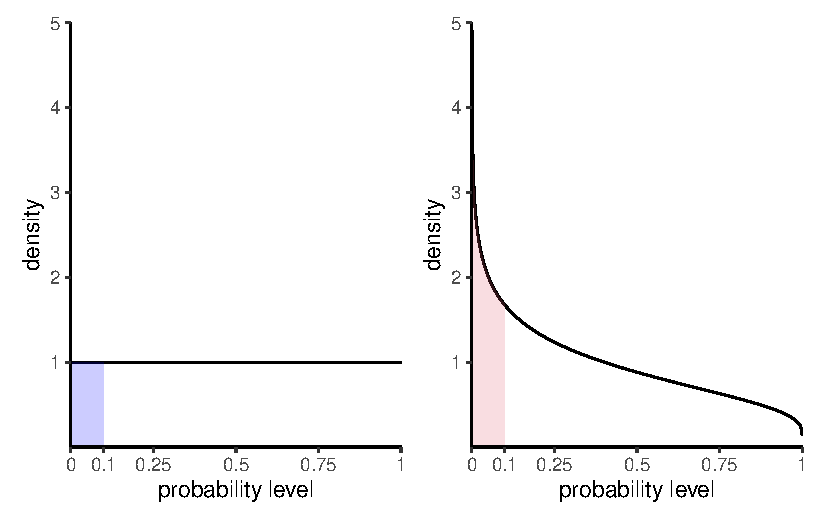
\includegraphics{02-hypothesis_testing_files/figure-pdf/fig-power-plots-1.pdf}

}

\caption{\label{fig-power-plots}Density of \emph{p}-values under the
null hypothesis (left) and under an alternative with a signal-to-noise
ratio of 0.5 (right).}

\end{figure}

There are generally three ways of obtaining null distributions for
assessing the degree of evidence against the null hypothesis

\begin{itemize}
\tightlist
\item
  exact calculations
\item
  large sample theory (aka `asymptotics' in statistical lingo)
\item
  simulation
\end{itemize}

While desirable, the first method is only applicable in simple cases
(such as counting the probability of getting two six if you throw two
fair die). The second method is most commonly used due to its generality
and ease of use (particularly in older times where computing power was
scarce), but fares poorly with small sample sizes (where `too small' is
context and test-dependent). The last approach can be used to
approximate the null distribution in many scenarios, but adds a layer of
randomness and the extra computations costs sometimes are not worth it.

\hypertarget{conclusion}{%
\subsection{Conclusion}\label{conclusion}}

The \emph{p}-value allows us to make a decision about the null
hypothesis. If \(\mathscr{H}_0\) is true, the \emph{p}-value follows a
uniform distribution, as shown in Figure~\ref{fig-power-plots}.
\href{https://xkcd.com/1478/}{Thus, if the \emph{p}-value is small},
this means observing an outcome more extreme than \(T=t\) is unlikely,
and so we're inclined to think that \(\mathscr{H}_0\) is not true.
There's always some underlying risk that we're making a mistake when we
make a decision. In statistic, there are
\href{https://xkcd.com/2303/}{two type of errors}:

\begin{itemize}
\tightlist
\item
  type I error: we reject the null hypothesis \(\mathscr{H}_0\) when the
  null is true,
\item
  type II error: we fail to reject the null hypothesis \(\mathscr{H}_0\)
  when the alternative is true.
\end{itemize}

The two hypothesis are not judged equally: we seek to avoid error of
type I (judicial errors, corresponding to condamning an innocent). To
prevent this, we fix a the level of the test, \(\alpha\), which captures
our tolerance to the risk of commiting a type I error: the higher the
level of the test \(\alpha\), the more often we will reject the null
hypothesis when the latter is true. The value of \(\alpha \in (0, 1)\)
is the probability of rejecting \(\mathscr{H}_0\) when \(\mathscr{H}_0\)
is in fact true, \begin{align*}
\alpha = \mathsf{Pr}_0\left(\text{ reject } \mathscr{H}_0\right).
\end{align*} The level \(\alpha\) is fixed beforehand, typically
\(1\)\%, \(5\)\% or \(10\)\%. Keep in mind that the probability of type
I error is \(\alpha\) only if the null model for \(\mathscr{H}_0\) is
correct (sic) and correspond to the data generating mechanism.

The focus on type I error is best understood by thinking about costs of
moving away from the status quo: a new website design or branding will
be costly to implement, so you want to make sure there are enough
evidence that the proposal is the better alternative and will lead to
increased traffic or revenues.

\begin{longtable}[]{@{}lcc@{}}
\toprule\noalign{}
\textbf{Decision} \textbackslash{} \textbf{true model} &
\(\mathscr{H}_0\) & \(\mathscr{H}_a\) \\
\midrule\noalign{}
\endhead
\bottomrule\noalign{}
\endlastfoot
fail to reject \(\mathscr{H}_0\) & \(\checkmark\) & type II error \\
reject \(\mathscr{H}_0\) & type I error & \(\checkmark\) \\
\end{longtable}

To make a decision, we compare our \emph{p}-value \(P\) with the level
of the test \(\alpha\):

\begin{itemize}
\tightlist
\item
  if \(P < \alpha\), we reject \(\mathscr{H}_0\);
\item
  if \(P \geq \alpha\), we fail to reject \(\mathscr{H}_0\).
\end{itemize}

Do not mix up level of the test (a probability fixed beforehand by the
researcher) and the \emph{p}-value. If you do a test at level 5\%, the
probability of type I error (condemning an innocent by mistake) is by
definition \(\alpha\) and does not depend on the \emph{p}-value. The
latter is a conditional probability of observing a more extreme
statistic given the null distribution \(\mathscr{H}_0\) is true.

\begin{tcolorbox}[enhanced jigsaw, colback=white, coltitle=black, rightrule=.15mm, left=2mm, bottomrule=.15mm, toprule=.15mm, titlerule=0mm, colframe=quarto-callout-caution-color-frame, leftrule=.75mm, title=\textcolor{quarto-callout-caution-color}{\faFire}\hspace{0.5em}{Pitfall}, breakable, arc=.35mm, colbacktitle=quarto-callout-caution-color!10!white, opacitybacktitle=0.6, opacityback=0, toptitle=1mm, bottomtitle=1mm]

The \href{https://doi.org/10.1080/00031305.2016.1154108}{American
Statistical Association (ASA) published a list of principles} guiding
(mis)interpretation of \emph{p}-values, some of which are reproduced
below:

\begin{quote}
\begin{enumerate}
\def\labelenumi{(\arabic{enumi})}
\setcounter{enumi}{1}
\tightlist
\item
  \emph{P}-values do not measure the probability that the studied
  hypothesis is true.
\end{enumerate}
\end{quote}

\begin{quote}
\begin{enumerate}
\def\labelenumi{(\arabic{enumi})}
\setcounter{enumi}{2}
\tightlist
\item
  Scientific conclusions and business or policy decisions should not be
  based only on whether a \emph{p}-value passes a specific threshold.
\end{enumerate}
\end{quote}

\begin{quote}
\begin{enumerate}
\def\labelenumi{(\arabic{enumi})}
\setcounter{enumi}{3}
\tightlist
\item
  \emph{P}-values and related analyses should not be reported
  selectively.
\end{enumerate}
\end{quote}

\begin{quote}
\begin{enumerate}
\def\labelenumi{(\arabic{enumi})}
\setcounter{enumi}{4}
\tightlist
\item
  \emph{p}-value, or statistical significance, does not measure the size
  of an effect or the importance of a result.
\end{enumerate}
\end{quote}

\end{tcolorbox}

\begin{example}[Gender inequality and permutation
tests]\protect\hypertarget{exm-rosenjerdee74}{}\label{exm-rosenjerdee74}

We consider data from Rosen and Jerdee (1974), who look at sex role
stereotypes and their impacts on promotion and opportunities for women
candidates. The experiment took place in 1972 and the experimental
units, which consisted of 95 male bank supervisors, were submitted to
various memorandums and asked to provide ratings or decisions based on
the information provided.

We are interested in Experiment 1 related to promotion of employees:
managers were requested to decide on whether or not to promote an
employee to become branch manager based on recommendations and ratings
on potential for customer and employee relations.

The authors intervention focused on the description of the nature
(complexity) of the manager's job (either simple or complex) and the sex
of the candidate (male or female): all files were otherwise similar.

We consider for simplicity only sex as a factor and aggregate over job
for the \(n=93\) replies. Table~\ref{tbl-rosen-table1} shows the counts
for each possibility.

\hypertarget{tbl-rosen-table1}{}
\begin{table}
\caption{\label{tbl-rosen-table1}Promotion recommandation to branch manager based on sex of the
applicant. }\tabularnewline

\centering
\begin{tabular}{lrr}
\toprule
  & male & female\\
\midrule
promote & 32 & 19\\
hold file & 12 & 30\\
\bottomrule
\end{tabular}
\end{table}

The null hypothesis of interest here that sex has no impact, so the
probability of promotion is the same for men and women. Let
\(p_{\text{m}}\) and \(p_{\text{w}}\) denote these respective
probabilities; we can thus write mathematically the null hypothesis as
\(\mathscr{H}_0: p_{\text{m}} = p_{\text{w}}\) against the alternative
\(\mathscr{H}_a: p_{\text{m}} \neq p_{\text{w}}\).

The test statistic typically employed for contingency tables is a
chi-square test\footnote{If you have taken advanced modelling courses,
  this is a score test obtained by fitting a Poisson regression with
  \texttt{sex} and \texttt{action} as covariates; the null hypothesis
  corresponding to lack of interaction term between the two.}, which
compares the overall proportions of promoted to that in for each
subgroup. The sample proportion for male is 32/42 = \textasciitilde76\%,
compared to 19/49 or \textasciitilde49\% for female. While it seems that
this difference of 16\% is large, it could be spurious: the standard
error for the sample proportions is roughly 3.2\% for male and 3.4\% for
female.

If there was no discrimination based on sex, we would expect the
proportion of people promoted to be the same overall; this is 51/93
=0.55 for the pooled sample. We could simply do a test for the mean
difference, but rely instead on the Pearson contingency \(X^2_p\) (aka
chi-square) test, which compares the expected counts (based on equal
promotion rates) to the observed counts, suitably standardized. If the
discrepancy is large between expected and observed, than this casts
doubt on the validity of the null hypothesis.

If the counts of each cell are large, the null distribution of the
chi-square test is well approximated by a \(\chi^2\) distribution. The
output of the test includes the value of the statistic, \(10.79\), the
degrees of freedom of the \(\chi^2\) approximation and the
\emph{p}-value, which gives the probability that a random draw from a
\(\chi^2_1\) distribution is larger than the observed test statistic
\textbf{assuming the null hypothesis is true}. The \emph{p}-value is
very small, \(0.001\), which means such a result is quite unlikely to
happen by chance if there was no sex-discrimination.

Another alternative to obtain a benchmark to assess the outlyingness of
the observed odds ratio is to use simulations. Consider a database
containing the raw data with 93 rows, one for each manager, with for
each an indicator of \texttt{action} and the \texttt{sex} of the
hypothetical employee presented in the task.

\hypertarget{tbl-dat-long-test-rosen-print}{}
\begin{table}
\caption{\label{tbl-dat-long-test-rosen-print}First five rows of the database in long format for experiment 1 of Rosen
and Jerdee. }\tabularnewline

\centering
\begin{tabular}{ll}
\toprule
action & sex\\
\midrule
hold file & female\\
promote & female\\
promote & male\\
hold file & female\\
hold file & female\\
\bottomrule
\end{tabular}
\end{table}

Under the null hypothesis, sex has no incidence on the action of the
manager. This means we could get an idea of the ``what-if'' world by
shuffling the sex labels repeatedly. Thus, we could obtain a benchmark
by repeating the following steps multiple times:

\begin{enumerate}
\def\labelenumi{\arabic{enumi}.}
\tightlist
\item
  permute the labels for \texttt{sex},
\item
  recreate a contingency table by aggregating counts,
\item
  calculate a test statistic for the simulated table.
\end{enumerate}

As test statistic, we use odds ratio: the odds of an event is the ratio
of the number of success over failure: in our example, this would be the
number of promoted over held files. The odds of promotion for male is
\(32/12\), whereas that of female is \(19/30\). The odds ratio for male
versus female is thus \(\mathsf{OR}=(32/12) / (19/30)= 4.21\). Under the
null hypothesis, \(\mathscr{H}_0: \mathsf{OR}= 1\) (same probability of
being promoted) (why?)

\begin{figure}[ht!]

{\centering 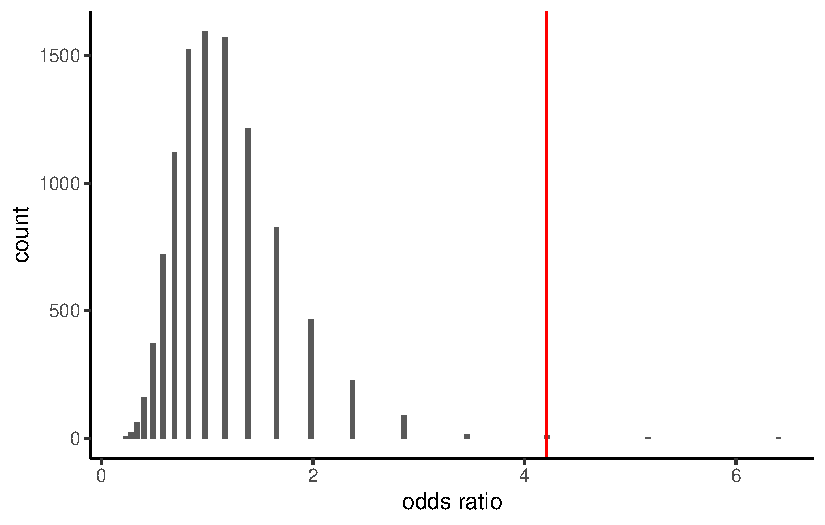
\includegraphics{02-hypothesis_testing_files/figure-pdf/fig-infer-odds-ratio-permutation-1.pdf}

}

\caption{\label{fig-infer-odds-ratio-permutation}Histogram of the
simulated null distribution of the odds ratio statistic obtained using a
permutation test; the vertical red line indicates the sample odds
ratio.}

\end{figure}

The histogram in Figure~\ref{fig-infer-odds-ratio-permutation} shows the
distribution of the odds ratio based on 10 000 permutations.
Reassuringly, we again get roughly the same approximate \emph{p}-value,
here 0.002.\footnote{The \emph{p}-value obtained for the permutation
  test would change from one run to the next since it's input is random.
  However, the precision of the proportion statistic is sufficient for
  decision making purposes.}

The article concluded (in light of the above and further experiments)

\begin{quote}
Results confirmed the hypothesis that male administrators tend to
discriminate against female employees in personnel decisions involving
promotion, development, and supervision.
\end{quote}

\textbf{Recap}

\begin{itemize}
\tightlist
\item
  Model parameters: probability of promotion for men and women,
  respectively \(p_{\text{m}}\) and \(p_{\text{w}}\).
\item
  Hypotheses: no discrimination based on gender, meaning equal
  probability of promotion (null hypothesis
  \(\mathscr{H}_0: p_{\text{m}}=p_{\text{w}}\), versus alternative
  hypothesis \(\mathscr{H}_a: p_{\text{m}}\neq p_{\text{w}}\)).
\item
  Test statistic: (1) chi-square test for contingency tables and (2)
  odds ratio.
\item
  \(p\)-value: (1) \(.0010\) and (2) \(.0024\) based on permutation
  test.
\item
  Conclusion: reject null hypothesis, as there is evidence of a
  gender-discrimination with different probability of promotion for men
  and women.
\end{itemize}

Following the APA guidelines, the \(\chi^2\) statistic would be reported
as \(\chi^2(1, n = 93) = 10.79\), \(p = .001\) along with counts and
sample proportions.

\end{example}

\begin{tcolorbox}[enhanced jigsaw, colback=white, coltitle=black, rightrule=.15mm, left=2mm, bottomrule=.15mm, toprule=.15mm, titlerule=0mm, colframe=quarto-callout-caution-color-frame, leftrule=.75mm, title=\textcolor{quarto-callout-caution-color}{\faFire}\hspace{0.5em}{Pitfall}, breakable, arc=.35mm, colbacktitle=quarto-callout-caution-color!10!white, opacitybacktitle=0.6, opacityback=0, toptitle=1mm, bottomtitle=1mm]

In the first experiment, managers were also asked to rank applications
on their potential for both employee and customer relations using a
Likert scale of six items ranging from (1) extremely unfavorable to (6)
extremely favorable. However, only the averages are reported in Table 1
along with (Rosen and Jerdee 1974)

\begin{quote}
Mean rating for the male candidate was 4.73 compared to a mean rating of
4.25 for the female candidate (\(F=4.76\), \(\text{df} = 1/80\),
\(p < .05\))
\end{quote}

The degrees of freedom (80) are much too few compared to the number of
observations, implying non-response that isn't discussed.

Partial or selective reporting of statistical procedures hinders
reproducibility. In general, the presentation should explicitly state
the name of the test statistic employed, the sample size, mean and
variance estimates, the null distribution used to assess significance
and its parameters, if any. Without these, we are left to speculate.

\end{tcolorbox}

\hypertarget{confidence-intervals}{%
\section{Confidence intervals}\label{confidence-intervals}}

A \textbf{confidence interval} is an alternative way to present the
conclusions of an hypothesis test performed at significance level
\(\alpha\) by giving a range of all values for which the null isn't
rejected at the chosen level. It is often combined with a point
estimator \(\hat{\theta}\) to give an indication of the variability of
the estimation procedure. Wald-based \((1-\alpha)\) confidence intervals
for a parameter \(\theta\) are of the form \begin{align*}
\widehat{\theta} + \text{critical value} \; \mathrm{se}(\widehat{\theta})
\end{align*} based on the Wald statistic \(W\), \begin{align*}
W =\frac{\widehat{\theta}-\theta}{\mathrm{se}(\widehat{\theta})},
\end{align*} and where \(\theta\) represents the postulated value for
the fixed, but unknown value of the parameter. The critical values are
quantile of the null distribution and are chosen so that the probability
of being more extreme is \(\alpha\).

The bounds of the confidence intervals are random variables, since both
estimators of the parameter and its standard error, \(\widehat{\theta}\)
and \(\mathrm{se}(\widehat{\theta})\), are random: their values will
vary from one sample to the next.

For generic random samples, there is a \(1-\alpha\) probability that
\(\theta\) is contained in the \textbf{random} confidence interval
computed. Once we obtain a sample and calculate the confidence interval,
there is no more notion of probability: the true value of the parameter
\(\theta\) is either inside the confidence interval or not. We can
interpret confidence interval's as follows: if we were to repeat the
experiment multiple times, and calculate a \(1-\alpha\) confidence
interval each time, then roughly \(1-\alpha\) of the calculated
confidence intervals would contain the true value of \(\theta\) in
repeated samples (in the same way, if you flip a coin, there is roughly
a 50-50 chance of getting heads or tails, but any outcome will be
either). Our confidence is in the \emph{procedure} we use to calculate
confidence intervals and not in the actual values we obtain from a
sample.

\begin{figure}[ht!]

{\centering 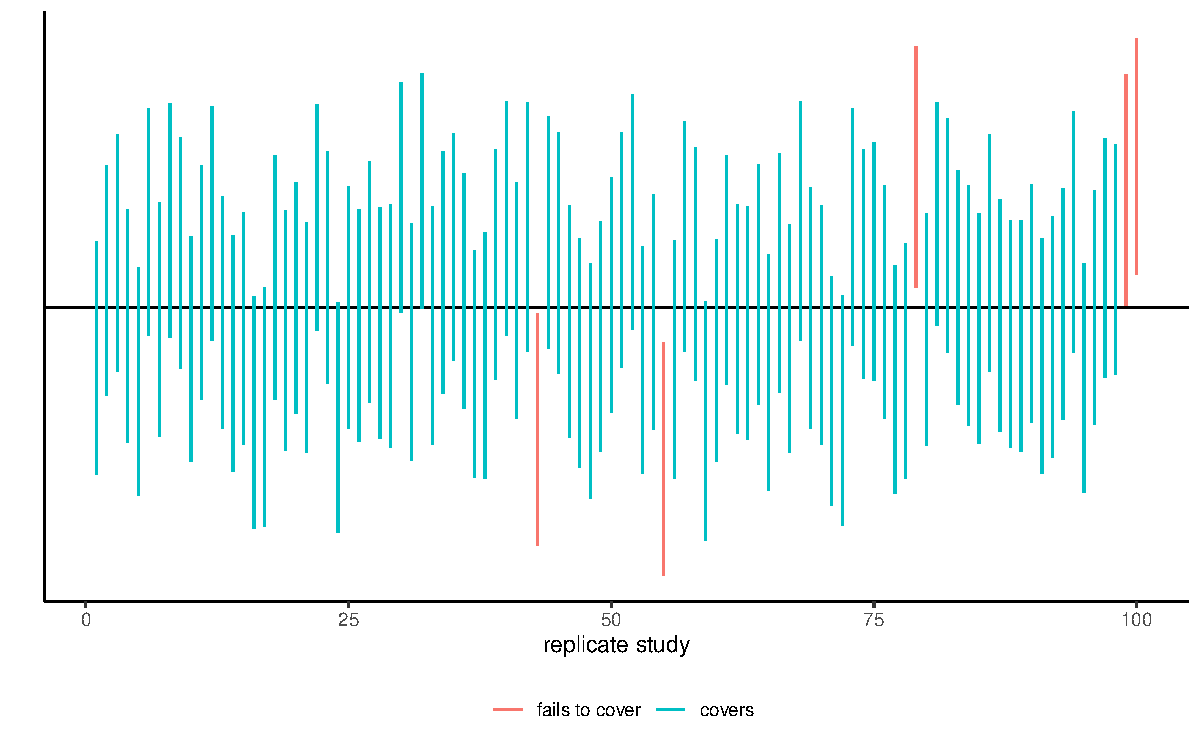
\includegraphics{02-hypothesis_testing_files/figure-pdf/intconf-1.pdf}

}

\caption{95\% confidence intervals for the mean of a standard normal
population for 100 random samples. On average, 5\% of these intervals
fail to include the true mean value of zero (in red).}

\end{figure}

If we are only interested in the binary decision rule reject/fail to
reject \(\mathscr{H}_0\), the confidence interval is equivalent to a
\emph{p}-value since it leads to the same conclusion. Whereas the
\(1-\alpha\) confidence interval gives the set of all values for which
the test statistic doesn't provide enough evidence to reject
\(\mathscr{H}_0\) at level \(\alpha\), the \emph{p}-value gives the
probability under the null of obtaining a result more extreme than the
postulated value and so is more precise for this particular value. If
the \emph{p}-value is smaller than \(\alpha\), our null value \(\theta\)
will be outside of the confidence interval and vice-versa.

\begin{example}[``The Surprise of Reaching
Out'']\protect\hypertarget{exm-LiuRimMinMin2023E1}{}\label{exm-LiuRimMinMin2023E1}

Liu et al. (2023) studies social interactions and the impact of surprise
on people reaching out if this contact is unexpected. Experiment 1
focuses on questionnaires where the experimental condition is the
perceived appreciation of reaching out to someone (vs being reached to).
The study used a questionnaire administered to 200 American adults
recruited on the Prolific Academic platform. The response index consists
of the average of four questions measured on a Likert scale ranging from
1 to 7, with higher values indicating higher appreciation.

\end{example}

We can begin by inspecting summary statistics for the sociodemographic
variables (gender and age) to assess whether the sample is
representative of the general population as a whole. The proportion of
\texttt{other} (including non-binary people) is much higher than that of
the general census, and the population skews quite young according to
Table~\ref{tbl-LRMMS1-summarystat-a}.

\hypertarget{tbl-LRMMS1-summarystat-a}{}
\begin{table}
\caption{\label{tbl-LRMMS1-summarystat-a}Summary statistics of the age of participants, and counts per gender }\tabularnewline

\centering
\begin{tabular}{lrrrr}
\toprule
gender & min & max & mean & n\\
\midrule
male & 18 & 78 & 32.03 & 105\\
female & 19 & 68 & 36.50 & 92\\
other & 24 & 30 & 27.67 & 3\\
\bottomrule
\end{tabular}
\end{table}

\hypertarget{tbl-LRMMS1-summarystat-b}{}
\begin{table}
\caption{\label{tbl-LRMMS1-summarystat-b}Mean ratings, standard deviation and number of participants per
experimental condition. }\tabularnewline

\centering
\begin{tabular}{lrrr}
\toprule
role & mean & sd & n\\
\midrule
initiator & 5.50 & 1.28 & 103\\
responder & 5.87 & 1.27 & 97\\
\bottomrule
\end{tabular}
\end{table}

Since there are only two groups, initiator and responder, we are dealing
with a pairwise comparison. The logical test one could use is a two
sample \emph{t}-test, or a variant thereof. Using Welch two sample
\(t\)-test statistic, both group average and standard deviation are
estimated using the data provided and the latter are used to build a
statistic. This explains the non-integer degrees of freedom.

The software returns \(t(197.52) = -2.05\), \(p = .041\), which leads to
the rejection of the null hypothesis of no difference in appreciation
depending on the role of the individual (initiator or responder). The
estimated mean difference is \(\Delta M = -0.37\), 95\% CI
\([-0.73, -0.01]\); since \(0\) is not included in the confidence
interval, we also reject the null hypothesis at level 5\%. The estimate
suggests that initiators underestimate the appreciation of reaching
out.\footnote{Assuming that the variance of each subgroup were equal, we
  could have used a two-sample \(t\)-test instead. The difference in the
  conclusion is immaterial, with a nearly equal \emph{p}-value.}

\textbf{Recap}

\begin{itemize}
\tightlist
\item
  Model parameters: average expected appreciation score
  \(\mu_{\mathrm{i}}\) and \(\mu_{\mathrm{r}}\) of initiators and
  responder, respectively
\item
  Hypothesis: expected appreciation score is the same for initiator and
  responders, \(\mathscr{H}_0: \mu_{\mathrm{i}}=\mu_{\mathrm{r}}\)
  against alternative
  \(\mathscr{H}_0: \mu_{\mathrm{i}} \neq \mu_{\mathrm{r}}\) that they
  are different.
\item
  Test statistic: Welch two sample \(t\)-test
\item
  \(p\)-value: 0.041
\item
  Conclusion: reject the null hypothesis, average appreciation score
  differs depending on the role
\end{itemize}

\begin{example}[Virtual communication curbs creative idea
generation]\protect\hypertarget{exm-BrucksLevav22}{}\label{exm-BrucksLevav22}

A Nature study performed an experiment to see how virtual communications
teamwork by comparing the output both in terms of ideas generated during
a brainstorming session by pairs and of the quality of ideas, as
measured by external referees. The sample consisted of 301 pairs of
participants who interacted via either videoconference or face-to-face.

The authors compared the number of creative ideas, a subset of the ideas
generated with creativity score above average. The mean number of the
number of creative ideas for face-to-face \(7.92\) ideas (sd \(3.40\))
relative to videoconferencing \(6.73\) ideas (sd \(3.27\)).

Brucks and Levav (2022) used a negative binomial regression model: in
their model, the expected number creative ideas generated is
\begin{align*}
\mathsf{E}(\texttt{ncreative}) = \exp(\beta_0 + \beta_1 \texttt{video})
\end{align*} where \(\texttt{video}=0\) if the pair are in the same room
and \(\texttt{video}=1\) if they interact instead via videoconferencing.

The mean number of ideas for videoconferencing is thus \(\exp(\beta_1)\)
times that of the face-to-face: the estimate of the multiplicative
factor is \(\exp(\beta_1)\) is \(0.85\) 95\% CI \([0.77, 0.94]\).

No difference between experimental conditions translates into the null
hypothesis as \(\mathscr{H}_0: \beta_1=0\) vs
\(\mathscr{H}_0: \beta_1 \neq 0\) or equivalently
\(\mathscr{H}_0: \exp(\beta_1)=1\). The likelihood ratio test comparing
the regression model with and without \(\texttt{video}\) the statistic
is \(R=9.89\) (\(p\)-value based on \(\chi^2_1\) of \(.002\)). We
conclude the average number of ideas is different, with summary
statistics suggesting that virtual pairs generate fewer ideas.

If we had resorted to a two sample \(t\)-test, we would have found a
mean difference in number of creative idea of \(\Delta M = 1.19\), 95\%
CI \([0.43, 1.95]\), \(t(299) = 3.09\), \(p = .002\).

Both tests come with slightly different sets of assumptions, but yield
similar conclusions: there is evidence of a smaller number of creative
ideas when people interact via videoconferencing.

\end{example}

\hypertarget{conclusion-1}{%
\section{Conclusion}\label{conclusion-1}}

This chapter has focused on presenting the tools of the trade and some
examples outlining the key ingredients that are common to any
statistical procedure and the reporting of the latter. The reader is not
expected to know which test statistic to adopt, but rather should
understand at this stage how our ability to do (scientific) discoveries
depends on a number of factors.

Richard McElreath in the
\href{http://xcelab.net/rmpubs/sr2/statisticalrethinking2_chapters1and2.pdf}{first
chapter} of his book (McElreath 2020) draws a parallel between
statistical tests and golems (i.e., robots): neither

\begin{quote}
discern when the context is inapropriate for its answers. It just knows
its own procedure {[}\ldots{]} It just does as it's told.
\end{quote}

The responsibility therefore lies with the user to correctly use
statistical procedures and be aware of their limitations. A
\emph{p}-value does not indicate whether the hypothesis is reasonable,
whether the design is proper, whether the choice of measurement is
adequate, etc.

\begin{tcolorbox}[enhanced jigsaw, colback=white, coltitle=black, rightrule=.15mm, left=2mm, bottomrule=.15mm, toprule=.15mm, titlerule=0mm, colframe=quarto-callout-tip-color-frame, leftrule=.75mm, title=\textcolor{quarto-callout-tip-color}{\faLightbulb}\hspace{0.5em}{Your turn}, breakable, arc=.35mm, colbacktitle=quarto-callout-tip-color!10!white, opacitybacktitle=0.6, opacityback=0, toptitle=1mm, bottomtitle=1mm]

Pick a journal paper (e.g., one of the dataset documented in the course
webpage) and a particular study.

Look up for the ingredients of the testing procedure (parameters,
hypotheses, test statistic name and value, summary statistics,
\emph{p}-value, conclusion).

You may encounter other measures, such as effect size, that will be
discussed later.

\end{tcolorbox}

\bookmarksetup{startatroot}

\hypertarget{CRT}{%
\chapter{Completely randomized designs}\label{CRT}}

This chapter focuses on experiments where potentially multiple factors
of interest are manipulated by the experimenter to study their impact.
If the allocation of observational units to each treatment combination
is completely random, the resulting experiment is a completely
randomized design.

The one-way analysis of variance describes the most simple experimental
setup one can consider: completely randomized experiments with one
factor, in which we are solely interested in the effect of a single
treatment variable with multiple levels.

\hypertarget{one-way-analysis-of-variance}{%
\section{One-way analysis of
variance}\label{one-way-analysis-of-variance}}

The focus is on comparisons of the average of a single outcome variable
with \(K\) different treatments levels, each defining a sub-population
differing only in the experimental condition they received. A
\textbf{one-way analysis of variance} compares the sample averages of
each treatment group \(T_1, \ldots, T_K\) to try and determine if the
population averages could be the same. Since we have \(K\) groups, there
will be \(K\) averages (one per group) to estimate.

Let \(\mu_1, \ldots, \mu_K\) denote the theoretical (unknown) mean (aka
expectation) of each of the \(K\) sub-populations defined by the
different treatments. Lack of difference between treatments is
equivalent to equality of means, which translates into the hypotheses
\begin{align*}
\mathscr{H}_0: & \mu_1 = \cdots = \mu_K \\
\mathscr{H}_a: & \text{at least two treatments have different averages, }
\end{align*} The null hypothesis is, as usual, a single numerical value,
\(\mu\). The alternative consists of all potential scenarios for which
not all expectations are equal. Going from \(K\) averages to one
requires imposing \(K-1\) restrictions (the number of equality signs),
as the value of the global mean \(\mu\) is left unspecified.

\hypertarget{parametrizations-and-contrasts}{%
\subsection{Parametrizations and
contrasts}\label{parametrizations-and-contrasts}}

This section can be skipped on first reading. It focuses on the
interpretation of the coefficients obtained from a linear model or
analysis of variance model.

The most natural parametrization is in terms of group averages: the
(theoretical unknown) average for treatment \(T_j\) is \(\mu_j\), so we
obtain \(K\) parameters \(\mu_1, \ldots, \mu_K\) whose estimates are the
sample averages \(\widehat{\mu}_1, \ldots, \widehat{\mu}_K\). One slight
complication arising from the above is that the values of the population
average are unknown, so this formulation is ill-suited for hypothesis
testing because none of the \(\mu_i\) values are known in practice and
we need to make comparisons in terms of a known numerical value.

The most common parametrization for the linear model is in terms of
\textbf{differences to a baseline}, say \(T_1\). The theoretical average
of each group is written as \(\mu_1 + a_i\) for treatment \(T_i\), where
\(a_1=0\) for \(T_1\) and \(a_i = \mu_i-\mu_1\) otherwise. The
parameters are \(\mu_1, a_2, \ldots, a_K\).

An equivalent formulation writes for each treatment group the average of
subpopulation \(j\) as \(\mu_j = \mu + \delta_j\), where \(\delta_j\) is
the difference between the treatment average \(\mu_j\) and the global
average of all groups. Imposing the constraint
\(\delta_1 + \cdots + \delta_K=0\) ensures that the average of effects
equals \(\mu\). Thus, if we know any \(K-1\) of
\(\{\delta_1, \ldots, \delta_K\}\), we automatically can deduce the last
one.

\begin{example}[Impact of encouragement on
teaching]\protect\hypertarget{exm-teaching1}{}\label{exm-teaching1}

In \textbf{R}, the \texttt{lm} function fits a linear model based on a
formula of the form \texttt{response\ \textasciitilde{}\ explanatory}.
If the explanatory is categorical (i.e., a factor), the parameters of
this model are the intercept, which is the sample average of the
baseline group and the other parameters are simply contrasts, i.e., the
\(a_i\)'s.

The sum-to-zero parametrization is obtained with
\texttt{contrasts\ =\ list(...\ =\ contr.sum)}, where the ellipsis is
replaced by the name of the categorical variable; an easier alternative
is \texttt{aov}, which enforces this parametrization by default. With
the sum-to-zero parametrization, the intercept is the average of each
treatment average, \((\widehat{\mu}_1 + \cdots + \widehat{\mu}_5)/5\);
this need not coincide with the (overall) mean of the response
\(\widehat{\mu} = \overline{y}\) unless the sample the number of
observations in each group is the same.\footnote{We say a sample is
  balanced if each (sub)group contains the same number of observations.}
The other coefficients of the sum-to-zero parametrization are the
differences between this intercept and the group means.

We show the function call to fit a one-way ANOVA in the different
parametrizations along with the sample average of each arithmetic group
(the two controls who were taught separately and the groups that were
praised, reproved and ignored in the third class). Note that the omitted
category changes depending on the parametrization.

\begin{Shaded}
\begin{Highlighting}[]
\NormalTok{mod\_contrast }\OtherTok{\textless{}{-}} \FunctionTok{lm}\NormalTok{(score }\SpecialCharTok{\textasciitilde{}}\NormalTok{ group, }
                   \AttributeTok{data =}\NormalTok{ arithmetic)}
\NormalTok{mod\_sum2zero }\OtherTok{\textless{}{-}} \FunctionTok{lm}\NormalTok{(score }\SpecialCharTok{\textasciitilde{}}\NormalTok{ group, }
                   \AttributeTok{data =}\NormalTok{ arithmetic,}
                   \AttributeTok{contrasts =} \FunctionTok{list}\NormalTok{(}\AttributeTok{group =}\NormalTok{ contr.sum))}
\end{Highlighting}
\end{Shaded}

\hypertarget{tbl-tableanovaparam}{}
\begin{table}
\caption{\label{tbl-tableanovaparam}Coefficients of the analysis of variance model for the arithmetic scores
using different parametrizations. }\tabularnewline

\centering
\begin{tabular}{lrrr}
\toprule
group & mean & contrasts & sum-to-zero\\
\midrule
intercept &  & 19.67 & 21.00\\
control 1 & 19.67 &  & -1.33\\
control 2 & 18.33 & -1.33 & -2.67\\
praise & 27.44 & 7.78 & 6.44\\
reprove & 23.44 & 3.78 & 2.44\\
\addlinespace
ignore & 16.11 & -3.56 & \\
\bottomrule
\end{tabular}
\end{table}

\end{example}

We can still assess the hypothesis by comparing the sample means in each
group, which are noisy estimates of the population mean: their inherent
variability will limit our ability to detect differences in averages if
the signal-to-noise ratio is small.

\hypertarget{sum-of-squares-decomposition}{%
\subsection{Sum of squares
decomposition}\label{sum-of-squares-decomposition}}

The following section can be safely skipped on first reading: it
attempts to shed some light into how the \(F\)-test statistic works as a
summary of evidence, as it isn't straightforward in the way it appears.

The usual notation for the sum of squares decomposition is as follows:
suppose \(y_{ik}\) represents the \(i\)th person in the \(k\)th
treatment group (\(k=1, \ldots, K\)) and the sample size \(n\) can be
split between groups as \(n_1, \ldots, n_K\); in the case of a balanced
sample, \(n_1=\cdots=n_K = n/K\) and the number of observations in each
group is the same. We denote by \(\widehat{\mu}_k\) the sample average
in group \(k\) and \(\widehat{\mu}\) the overall average
\((y_{11} + \cdots + y_{n_KK})/n = \sum_k \sum_i y_{ik}/n\), where
\(\sum_i\) denotes the sum over all individuals in the group.

Under the null model, all groups have the same mean, so the natural
estimator for the latter is the sample average of the pooled sample
\(\widehat{\mu}\) and likewise the group averages
\(\widehat{\mu}_1, \ldots, \widehat{\mu}_K\) are the best estimators for
the group averages if each group has a (potentially) different mean. The
more complex model, which has more parameters, will always fit better
because it has more possibility to accommodate differences observed in a
group, even if these are spurious. The sum of squares measures the
(squared) distance between the observation and the fitted values, with
the terminology total, within and between sum of squares linked to the
decomposition \begin{align*}
\underset{\text{total sum of squares} }{\sum_{i}\sum_{k} (y_{ik} - \widehat{\mu})^2} &= \underset{\text{within sum of squares} }{\sum_i \sum_k (y_{ik} - \widehat{\mu}_k)^2} +  \underset{\text{between sum of squares} }{\sum_k n_i (\widehat{\mu}_k - \widehat{\mu})^2}.
\end{align*} The term on the left is a measure of the variability for
the null model \((\mu_1 = \cdots = \mu_K)\) under which all observations
are predicted by the overall average \(\widehat{\mu}\). The within sum
of squares measures the distance between observations and their group
mean, which describes the alternative model in which each group has
(potentially) a different average, but the same variability.

We can measure how much worst we do with the alternative model
(different average per group) relative to the null by calculating the
between sum of square. This quantity in itself varies with the sample
size (the more observations, the larger it is) so we must standardize as
usual this quantity so that we have a suitable benchmark.

The \(F\)-statistic is

\begin{equation}\protect\hypertarget{eq-Fstatheuristic}{}{
\begin{split}
F &= \frac{\text{between-group variability}}{\text{within-group variability}} \\
&= \frac{\text{between sum of squares}/(K-1)}{\text{within sum of squares}/(n-K)} 
\end{split}
}\label{eq-Fstatheuristic}\end{equation}

If there is no mean difference (null hypothesis), the numerator is an
estimator of the population variance, and so is the denominator of eq.
\ref{eq-Fstatheuristic} and the ratio of the two is approximately 1 on
average. However, the between sum of square is more variable and this
induces skewness: for large enough sample, the null distribution of the
\emph{F}-statistic is approximately an \emph{F}-distribution, whose
shape is governed by two parameters named degrees of freedom which
appear in Equation~\ref{eq-Fstatheuristic} as scaling factors to ensure
proper standardization. The first degree of freedom is the number of
restrictions imposed by the null hypothesis (\(K-1\), the number of
groups minus one for the one-way analysis of variance), and the second
degree of freedom is the number of observations minus the number of
\emph{parameters estimates} for the mean (\(n-K\), where \(n\) is the
overall sample size and \(K\) is the number of groups).\footnote{There
  are only \(K\) parameter estimates for the mean, since the overall
  mean is full determined by the other averages with
  \(n\widehat{\mu} =n_1\widehat{\mu}_1 + \cdots + n_K \widehat{\mu}_K\).}

Figure~\ref{fig-squareddistanova} shows how the difference between these
distances can encompass information that the null is wrong. The sum of
squares is obtained by computing the squared length of these vectors and
adding them up. The left panel shows strong signal-to-noise ratio, so
that, on average, the black segments are much longer than the colored
ones. This indicates that the model obtained by letting each group have
its own mean is much better than the other. The picture in the right
panel is not as clear: on average, the colored arrows are shorter, but
the difference in length is much smaller relative to the colored arrows.

\begin{figure}[ht!]

{\centering 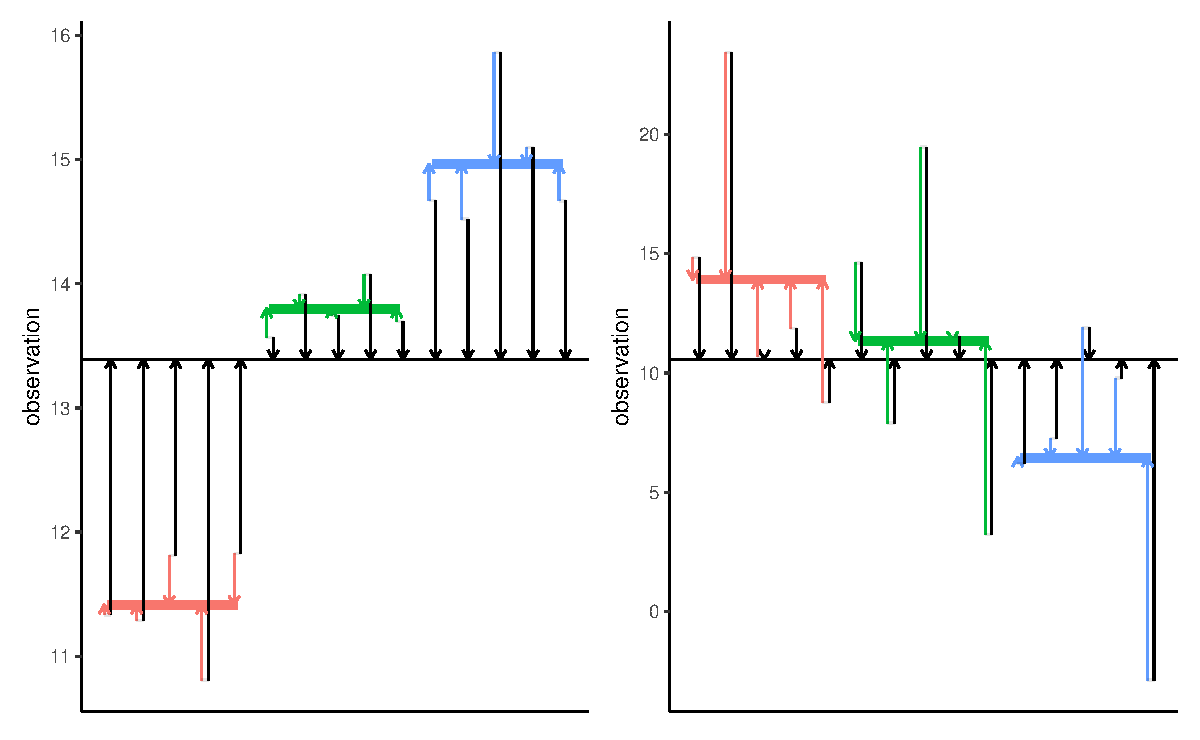
\includegraphics{03-completely_randomized_trials_files/figure-pdf/fig-squareddistanova-1.pdf}

}

\caption{\label{fig-squareddistanova}Observations drawn from three
groups from a model with a strong (left) and weak (right)
signal-to-noise ratio, along with their sample mean (colored horizontal
segments) and the overall average (horizontal line). Arrows indicate the
magnitude of the difference between the observation and the
(group/average) mean.}

\end{figure}

The \(F\)-distribution is what we call a \textbf{large sample
approximation} to the behaviour of the statistic if there is truly no
difference between group averages (and if model assumptions are
satisfied): it tells us what to expect if there is nothing going on. The
quality of the approximation depends on the sample size in each group:
it is more accurate when there are more observations in each group, as
average estimation becomes more reliable\footnote{Mostly because the
  central limit theorem kicks in}.

As was alluded to in the last chapter, large sample approximations are
not the only option for assessing the null, but they are cheap and easy
to obtain. If the distributions are the same under the null and
alternative except for a location shift, we could instead resort to a
permutation-based approach to
\href{https://www.jwilber.me/permutationtest/}{generate those
alternative samples by simply shuffling the labels}. We see in
Figure~\ref{fig-Fdistpermut} that the histogram of the \(F\)-statistic
values obtained from 1000 permutations closely matches that of the
large-sample \(F\)-distribution when there are on average 20
observations per group (right), so the computational burden associated
with running this simulation outweights the benefits. However, with
smaller samples (left), the large sample approximation appears
underdispersed relative to the permutation-based distribution, with more
extreme outcomes; the latter should be viewed as more accurate in this
setting.

\begin{figure}[ht!]

{\centering 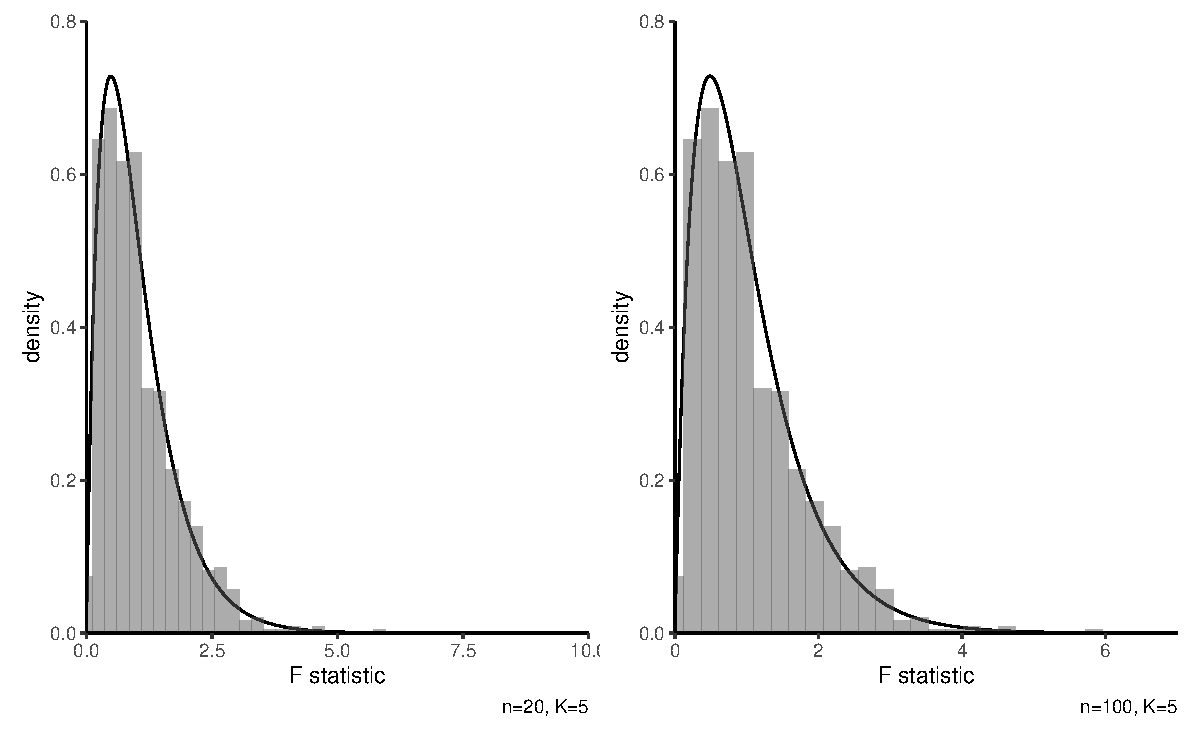
\includegraphics{03-completely_randomized_trials_files/figure-pdf/fig-Fdistpermut-1.pdf}

}

\caption{\label{fig-Fdistpermut}One-way analysis of variance for a
sample of size 20 (left) and 100 (right), split in five groups. The
histograms shows the computed test values based on 1000 permutations,
which are compared to the density of the large-sample
\emph{F}-distribution.}

\end{figure}

More interestingly perhaps is what happens to the values taken by the
statistic when not all of the averages are the same. We can see in
Figure~\ref{fig-distributionFanova} that, when there are some difference
between group means, the values taken by the statistic for a random
sample are more to the right than the null distribution: the larger
those differences, the more the curve will shift to the right and the
more often we will obtain a value in the rejection region (in red).

If there are only two groups, then one can show that the \(F\)-statistic
is mathematically equivalent to squaring the \(t\)-statistic: the null
distributions are \(\mathsf{St}(n-K)\) and \(\mathsf{F}(1, n-K)\) and
lead to the same \(p\)-values and thus same statistical inference and
conclusions.

\begin{figure}[ht!]

{\centering 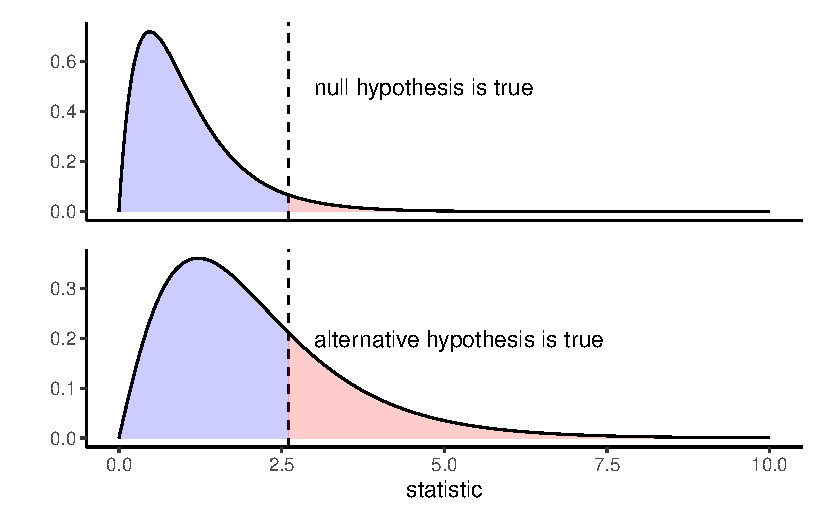
\includegraphics{03-completely_randomized_trials_files/figure-pdf/fig-distributionFanova-1.pdf}

}

\caption{\label{fig-distributionFanova}Distribution of the \(F\)-test
statistic for the one-way analysis of variance when the true group means
are equal (top) and under a specific alternative when they are not
(bottom). Any value falling within the red region leads to rejection of
the null hypothesis at level \(\alpha=0.05\).}

\end{figure}

\hypertarget{graphical-representation}{%
\section{Graphical representation}\label{graphical-representation}}

How to represent data for a one-way analysis in a publication? The
purpose of the visualization is to provide intuition that extends beyond
the reported descriptive statistics and to check the model assumptions.
Most of the time, we will be interested in averages and dispersion, but
plotting the raw data can be insightful. It is also important to keep in
mind that summary statistics are estimators of population quantities
that are perhaps unreliable (much too variable) in small samples to be
meaningful quantities. Since the mean estimates will likely be reported
in the text, the graphics should be used to convey additional
information about the data. If the samples are extremely large, then
graphics will be typically be used to present salient features of the
distributions.

\begin{figure}[ht!]

{\centering 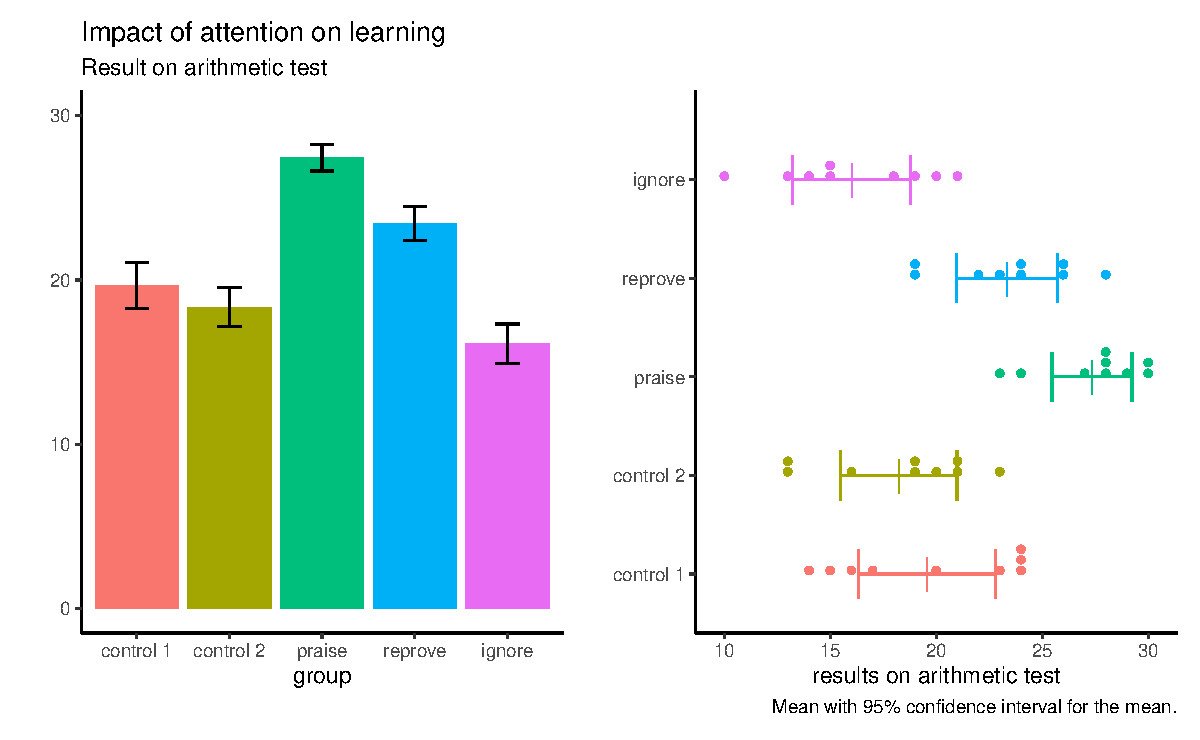
\includegraphics[width=0.9\textwidth,height=\textheight]{03-completely_randomized_trials_files/figure-pdf/fig-dynamiteplot-1.pdf}

}

\caption{\label{fig-dynamiteplot}Two graphical representations of the
arithmetic data: dynamite plot (left) showing the sample average with
one standard error above and below, and dot plot with the sample mean
(right).}

\end{figure}

In a one-way analysis of variance, the outcome is a continuous numerical
variable, whereas the treatment or explanatory is a categorical
variable. Basic graphics include dot plots, histograms and density
plots, or rugs for the raw data.

Typically, scatterplots are not a good option because observations get
overlaid. There are multiple workarounds, involving transparency, bubble
plots for discrete data with ties, adding noise (jitter) to every
observation or drawing values using a thin line (rugs) if the data are
continuous and take on few distinct values.

Journals are plagued with poor vizualisations, a prime example of which
is the infamous
\href{https://simplystatistics.org/2019/02/21/dynamite-plots-must-die/}{dynamite
plot}: it consists of a bar plot with one standard error interval. The
problem with this (or with other summary statistics) is that they hide
precious information about the spread and values taken by the data, as
many different data could give rise to the same average while being
quite different in nature. The height of the bar is the sample average
and the bars extend beyond one standard error: this makes little sense
as we end up comparing areas, whereas the mean is a single number. The
right panel of Figure~\ref{fig-dynamiteplot} shows instead a dot plot
for the data, i.e., sample values with ties stacked for clarity, along
with the sample average and a 95\% confidence interval for the latter as
a line underneath. In this example, there are not enough observations
per group to produce histograms, and a five number summary of nine
observations isn't really necessary so boxplot are useless. Weissgerber
et al. (2015) discusses alternative solutions and can be referenced when
fighting reviewers who insist on bad visualizations.

If we have a lot of data, it sometimes help to represent selected
summary statistics or group data. A box-and-whiskers plot (or boxplot)
is a commonly used graphic representing the whole data distribution
using five numbers

\begin{itemize}
\tightlist
\item
  The box gives the quartiles, say \(q_1\), \(q_2\) (median) and \(q_3\)
  of the distribution: 50\% of the observations are smaller or larger
  than \(q_2\), 25\% are smaller than \(q_1\) and 75\% are smaller than
  \(q_3\) for the sample.
\item
  The whiskers extend up to \(1.5\) times the box width (\(q_3-q_1\))
  (so the largest observation that is smaller than \(q_3+1.5(q_3-q_1)\),
  etc.)
\end{itemize}

Observations beyond the whiskers are represented by dots or circles,
sometimes termed outliers. However, beware of this terminology: the
larger the sample size, the more values will fall outside the whiskers
(about 0.7\% for normal data). This is a drawback of boxplots, which
were conceived at a time where big data didn't exist. If you want to
combine boxplots with the raw data, remove the display of outliers to
avoid artefacts.

\begin{figure}[ht!]

{\centering 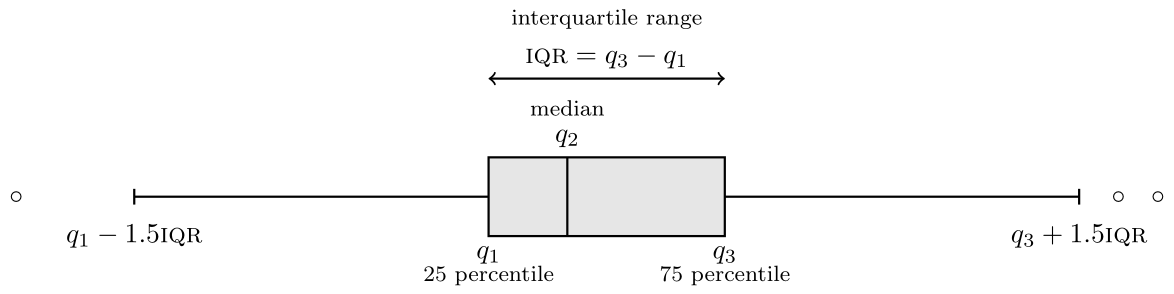
\includegraphics[width=0.8\textwidth,height=\textheight]{figures/01-intro-boxplot.png}

}

\caption{\label{fig-boxplot}Box-and-whiskers plot}

\end{figure}

Weissgerber et al. (2019) contains many examples of how to build
effective visualizations, including highlighting particular aspects
using color, jittering, transparency and how to adequately select the
display zone.

\hypertarget{pairwise-tests}{%
\section{Pairwise tests}\label{pairwise-tests}}

If the global test of equality of mean for the one-way ANOVA leads to
rejection of the null, the conclusion is that one of the group has a
different mean. However, the test does not indicate which of the groups
differ from the rest nor does it say how many are different. There are
different options: one is custom contrasts, a special instance of which
is pairwise comparisons.

We are interested in looking at the difference between the (population)
average of group \(i\) and \(j\), say. The null hypothesis of no
difference translate into \(\mu_i-\mu_j=0\), so the numerator of our
statistic will be the estimator \(\widehat{\mu}_i - \widehat{\mu}_j\) of
the difference in sample mean, minus zero.

Assuming equal variances, the two-sample \(t\)-test statistic is
\begin{align*}
t_{ij} = \frac{(\widehat{\mu}_i - \widehat{\mu}_j) - 0}{\mathsf{se}(\widehat{\mu}_i - \widehat{\mu}_j)} =\frac{\widehat{\mu}_i - \widehat{\mu}_j}{\widehat{\sigma} \left(\frac{1}{n_i} + \frac{1}{n_j}\right)^{1/2}},
\end{align*} where \(\widehat{\mu}_i\) and \(n_i\) are respectively the
sample average and the number of observations of group \(i\), and
\(\widehat{\sigma}\) is the estimator of the standard deviation derived
using the whole sample (assuming equal variance). As usual, the
denominator of \(t_{ij}\) is the standard error of the
\(\widehat{\mu}_i - \widehat{\mu}_j\), whose postulated difference is
zero. We can compare the value of the observed statistic to a
Student-\(t\) distribution with \(n-K\) degrees of freedom, denoted
\(\mathsf{St}(n-K)\). For a two-sided alternative, we reject if
\(|t_{ij}| > \mathfrak{t}_{1-\alpha/2}\), for
\(\mathfrak{t}_{1-\alpha/2}\) the \(1-\alpha/2\) quantile of
\(\mathsf{St}(n-K)\).

Figure~\ref{fig-tcurve} shows the density of the benchmark distribution
for pairwise comparisons in mean for the \texttt{arithmetic} data. The
blue area under the curve defines the set of values for which we fail to
reject the null hypothesis, whereas all values of the test statistic
falling in the red area lead to rejection at level \(5\)\%.

\begin{figure}[ht!]

{\centering 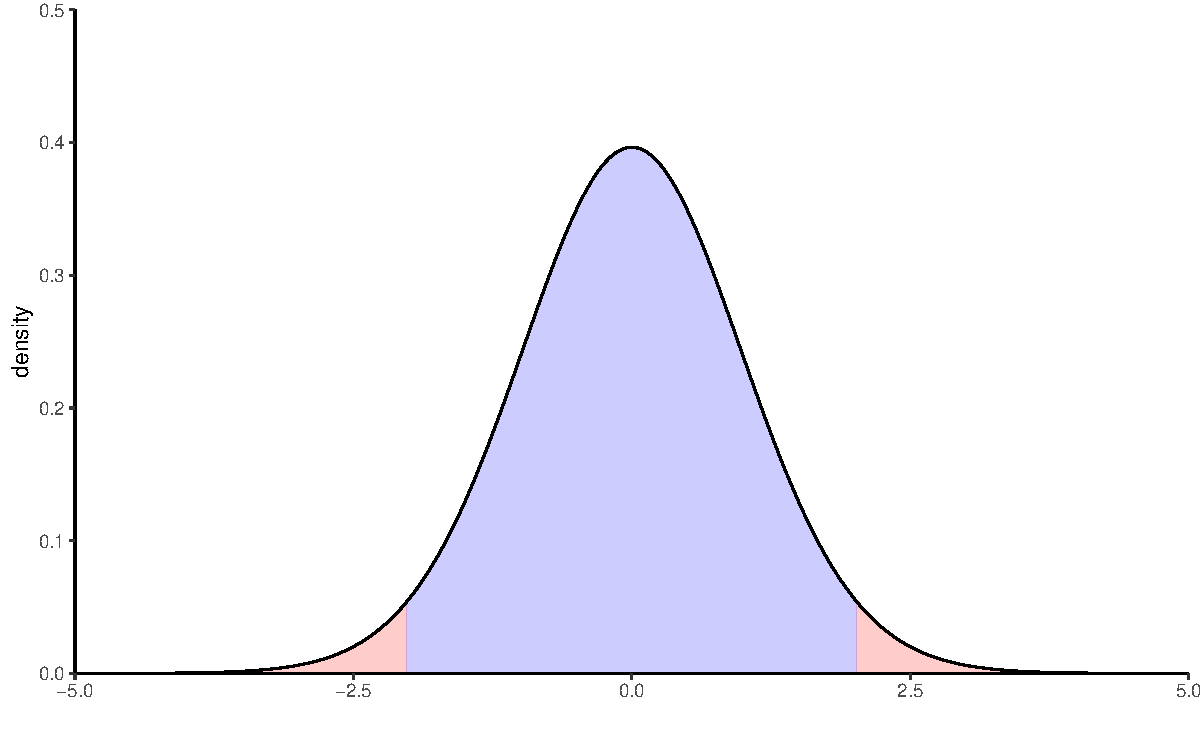
\includegraphics[width=0.8\textwidth,height=\textheight]{03-completely_randomized_trials_files/figure-pdf/fig-tcurve-1.pdf}

}

\caption{\label{fig-tcurve}Student-\emph{t} null distribution and
rejection region for a \emph{t}-test.}

\end{figure}

We fail to reject \(\mathscr{H}_0\) as
\(\mathfrak{t}_{\alpha/2} \leq t_{ij} \leq \mathfrak{t}_{1-\alpha/2}\)\footnote{Note
  that the Student-\(t\) distribution is symmetric, so
  \(\mathfrak{t}_{1-\alpha/2} = -\mathfrak{t}_{\alpha/2}\).}: this gives
us another way of presenting the same conclusion in terms of the set of
mean differences \(\delta_{ij} = \mu_i - \mu_j\) for which
\begin{align*}
 \mathfrak{t}_{\alpha/2} \leq \frac{\widehat{\delta}_{ij} - \delta_{ij}}{\mathsf{se}\left(\widehat{\delta}_{ij}\right)} \leq \mathfrak{t}_{1-\alpha/2}
\end{align*} which is equivalent upon rearranging to the \((1-\alpha)\)
confidence interval for \(\delta_{ij}\), \begin{align*}
\mathsf{CI} = \left[\widehat{\delta}_{ij} - \mathfrak{t}_{1-\alpha/2}\mathsf{se}\left(\widehat{\delta}_{ij}\right), \widehat{\delta}_{ij} - \mathfrak{t}_{\alpha/2}\mathsf{se}\left(\widehat{\delta}_{ij}\right)\right].
\end{align*}

\begin{example}[Calculation of pairwise
comparisons]\protect\hypertarget{exm-pairwise-calcul}{}\label{exm-pairwise-calcul}

We consider the pairwise average difference in scores between the
praised (group C) and the reproved (group D) of the \texttt{arithmetic}
study. The sample averages are respectively \(\widehat{\mu}_C = 27.4\)
and \(\widehat{\mu}_D = 23.4\) and the estimated pooled standard
deviation for the five groups is \(1.15\). Thus, the estimated average
difference between groups \(C\) and \(D\) is
\(\widehat{\delta}_{CD} = 4\) and the standard error for the difference
is \(\mathsf{se}(\widehat{\delta}_{CD}) = 1.6216\); all of these are
calculated by software.

If we take as null hypothesis \(\mathscr{H}_0: \delta_{CD}=0\), the
\(t\) statistic is
\begin{align*}t=\frac{\widehat{\delta}_{CD} - 0}{\mathsf{se}(\widehat{\delta}_{CD})} = \frac{4}{1.6216}=2.467
\end{align*} and the \(p\)-value is \(p=0.018\). We therefore reject the
null hypothesis at level \(\alpha=0.05\) to conclude that there is a
significant difference (at level \(\alpha=0.05\)) between the average
scores of students praised and reproved.

\end{example}

\hypertarget{model-assumptions}{%
\section{Model assumptions}\label{model-assumptions}}

So far, we have brushed all of the model assumptions under the carpet.
These are necessary requirements for the inference to be valid: any
statement related to \emph{p}-values, etc. will approximately hold only
if a set of assumptions is met in the first place. This section is
devoted to the discussion of these assumptions, showcasing examples of
where things can go wrong.

It is customary to write the \(i\)th observation of the \(k\)th group in
the one-way analysis of variance model as
\begin{equation}\protect\hypertarget{eq-onewayanova}{}{
\underset{\text{observation}}{Y_{ik}} = \underset{\text{mean of group $k$}}{\mu_k} + \underset{\text{error term}}{\varepsilon_{ik}},
}\label{eq-onewayanova}\end{equation} where the error terms
\(\varepsilon_{ik}\), which account for unexplained variability and
individual differences, are independent from one with mean zero and
variance \(\sigma^2\).

\hypertarget{additivity}{%
\subsection{Additivity}\label{additivity}}

The basic assumption of most designs is that we can decompose the
outcome into two components (Cox 1958)
\begin{equation}\protect\hypertarget{eq-additivefn}{}{
\begin{pmatrix} \text{quantity depending} \\
 \text{on the treatment used}\end{pmatrix} +
 \begin{pmatrix} \text{quantity depending only } \\
\text{on the particular unit} 
\end{pmatrix}
}\label{eq-additivefn}\end{equation}

This \textbf{additive} decomposition further assumes that each unit is
unaffected by the treatment of the other units and that the average
effect of the treatment is constant. Thus, it is justified to use
difference in sample mean to estimate the treatment effect since on
average, the individual effect is zero.

The decomposition of observations in terms of group average and
mean-zero noise in Equation~\ref{eq-onewayanova} suggests that we could
plot the error term \(\varepsilon_{ik}\) against observations, or
against other factors or explanatories, to see if there is any unusual
structure unexplained by the model and indicating problems with the
randomization or additivity. However, we do not have access to
\(\varepsilon_{ik}\) since both the true group mean \(\mu_k\) and the
error \(\varepsilon_{ik}\) are unknown. However, a good proxy is the
\textbf{ordinary residual} \(e_{ik} = y_{ik} - \widehat{\mu}_k\) where
\(\widehat{\mu}_k\) is the sample mean of all observations in
experimental group \(k\). By construction, the sample mean of the
residuals will be zero, but local deviations may indicate violations of
the analysis (for example, plotting residuals against time could show a
learning effect).

Many graphical diagnostics use residuals, i.e., some variant of the
observations minus the group mean \(y_{ik} - \widehat{\mu}_k\), to look
for violation of the assumptions.

\begin{figure}[ht!]

{\centering 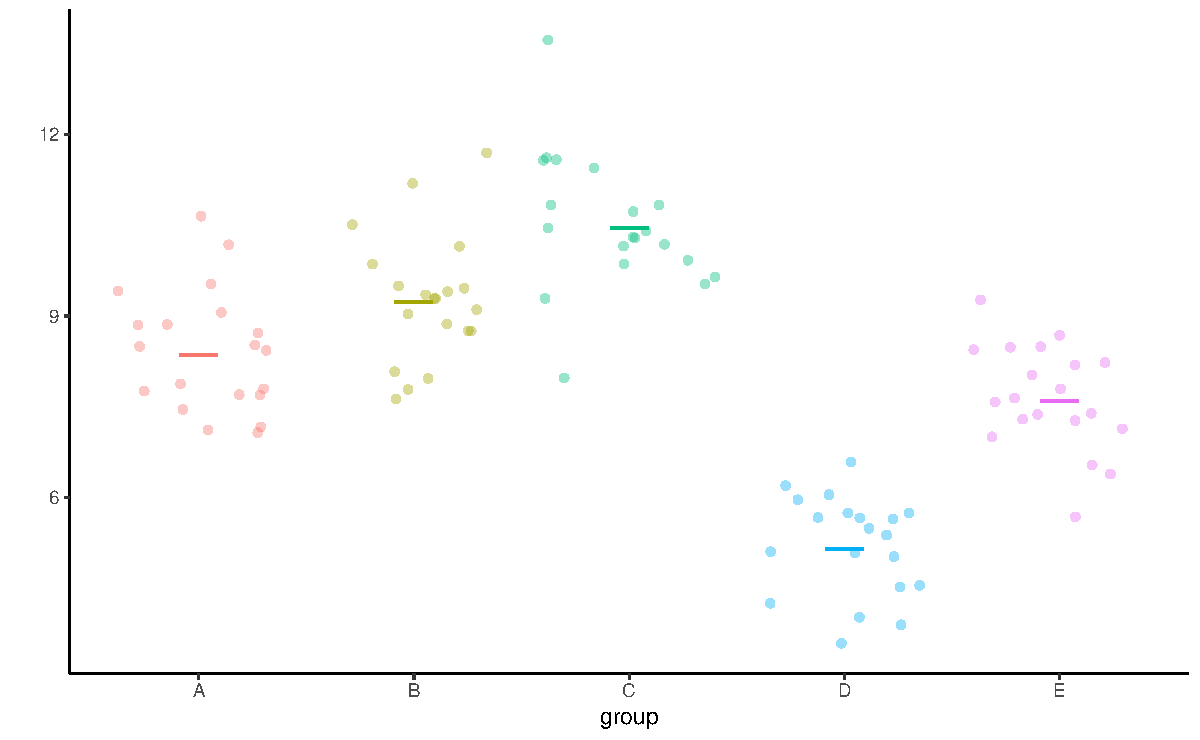
\includegraphics{03-completely_randomized_trials_files/figure-pdf/fig-assumptions-1.pdf}

}

\caption{\label{fig-assumptions}Data satisfying the assumptions of the
one-way analysis of variance model, with additive effects, independent
observations and common variance.}

\end{figure}

More generally, the test statistic may make further assumptions. The
\(F\)-test of the global null \(\mu_1 = \cdots \mu_K\) assumes that the
\(i\)th observation of group \(k\), say \(y_{ik}\), has average
\(\mathsf{E}(Y_{ik}) = \mu_k\) and variance
\(\mathsf{Va}(Y_{ik}) = \sigma^2\). The latter is estimated using all of
the residuals, with
\(\widehat{\sigma}^2 = \sum_k\sum_i (y_{ik} - \widehat{\mu}_k)^2/(n-K)\).
Under these assumptions, the \(F\)-test statistic for the global null
\(\mu_1 = \cdots = \mu_K\) is the most powerful because it uses all of
the data to get a more precise estimation of the variability. Generally,
there may be other considerations than power that may guide the choice
of test statistic, including robustness (sensitivity to extremes and
outliers). For unequal variance, other statistics than the \(F\)-test
statistic may be more powerful.

\begin{example}[Additivity and
transformations]\protect\hypertarget{exm-additivity-transfo}{}\label{exm-additivity-transfo}

Chapter 2 of Cox (1958) discusses the assumption of additivity and
provides useful examples showing when it cannot be taken for granted.
One of them, Example 2.3, is a scenario in which the experimental units
are participants and they are asked to provide a ranking of different
kindergarten students on their capacity to interact with others in
games, ranked on a scale of 0 to 100. A random group of students
receives additional orthopedagogical support, while the balance is in
the business-as-usual setting (control group). Since there are intrinsic
differences at the student level, one could consider a \textbf{paired
experiment} and take as outcome the difference in sociability scores at
the beginning and at the end of the school year.

One can expect the treatment to have more impact on people with low
sociability skills who were struggling to make contacts: a student who
scored 50 initially might see an improvement of 20 points with support
relative to 10 in the business-as-usual scenario, whereas another who is
well integrated and scored high initially may see an improvement of only
5 more had (s)he been assigned to the support group. This implies that
the treatment effects are not constant over the scale, a violation of
the additivity assumption. One way to deal with this is via
transformations: Cox (1958) discusses the transformation
\(\log\{(x+0.5)/(100.5-x)\}\) to reduce the warping due to scale.

\end{example}

Another example is in experiments where the effect of treatment is
multiplicative, so that the output is of the form \begin{align*}
\begin{pmatrix} \text{quantity depending only } \\ 
\text{on the particular unit} 
\end{pmatrix} \times
\begin{pmatrix} \text{quantity depending} \\
 \text{on the treatment used}\end{pmatrix}
\end{align*} Usually, this arises for positive responses and treatments,
in which case taking natural logarithms on both sides, with
\(\log(xy) = \log x + \log y\) yielding again an additive decomposition.

\begin{example}[Inadequacy of additivity based on
context]\protect\hypertarget{exm-additivity-context}{}\label{exm-additivity-context}

This example is adapted from Cox (1958), Example 2.2. Children suffering
from attention deficit hyperactivity disorder (ADHD) may receive
medication to increase their attention span, measured on a scale of 0 to
100, with 0 indicating normal attention span. An experiment can be
designed to assess the impact of a standardized dose in a laboratory by
comparing performances of students on a series of task before and after,
when to a placebo. To make a case, suppose that students with ADHD fall
into two categories: low symptoms and strong symptoms. In the low
symptom group, the average attention is 8 per cent with the drug and 12
per cent with the placebo, whereas for people with strong symptoms, the
average is 40 per cent among treated and 60 per cent with the placebo.
If these two categories are equally represented in the experiment and
the population, we would estimate an average reduction of 12 percent in
the score (thus higher attention span among treated). Yet, this quantity
is artificial, and a better measure would be that symptoms are for the
treatment are 2/3 of those of the control (the ratio of proportions).

\end{example}

Equation~\ref{eq-additivefn} also implies that the effect of the
treatment is constant for all individuals. This often isn't the case: in
an experimental study on the impact of teaching delivery type (online,
hybrid, in person), it may be that the response to the choice of
delivery mode depends on the different preferences of learning types
(auditory, visual, kinestetic, etc.) Thus, recording additional
measurements that are susceptible to interact may be useful; likewise,
treatment allotment must factor in this variability should we wish to
make it detectable. The solution to this would be to setup a more
complex model (two-way analysis of variance, general linear model) or
stratify by the explanatory variable (for example, compute the
difference within each level).

\begin{figure}[ht!]

{\centering 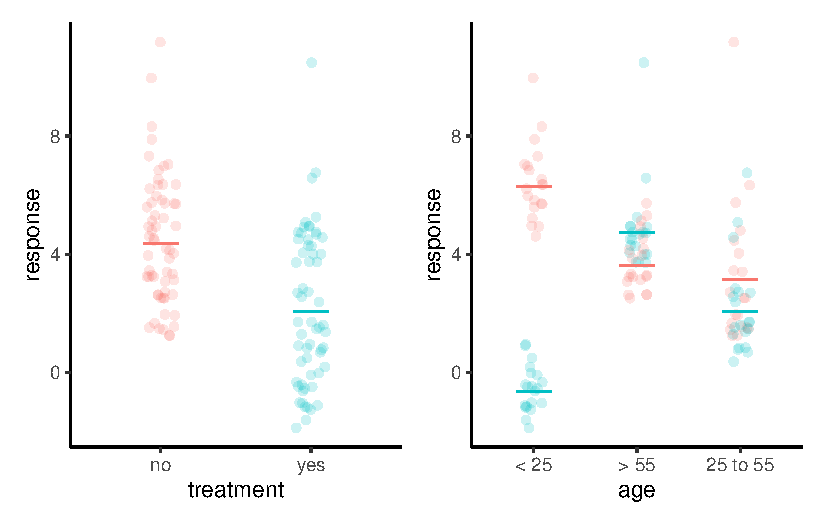
\includegraphics{03-completely_randomized_trials_files/figure-pdf/fig-omittedlinearity-1.pdf}

}

\caption{\label{fig-omittedlinearity}Difference in average response;
while the treatment seems to lead to a decrease in the response
variable, a stratification by age group reveals this only occurs in the
younger population aged less than 25 years, with a seemingly reversed
effect for the older adults. Thus, the marginal model implied by the
one-way analysis of variance is misleading.}

\end{figure}

\hypertarget{heterogeneity}{%
\subsection{Heterogeneity}\label{heterogeneity}}

The one-way ANOVA builds on the fact that the variance in each group is
equal, so that upon recentering, we can estimate it from the variance of
the residuals \(y_{ik} - \widehat{\mu}_k\). Specifically, the unbiased
variance estimator is the denominator of the \(F\)-statistic formula,
i.e., the within sum of squares divided by \(n-K\) with \(n\) the total
number of observations and \(K\) the number of groups under comparison.

For the time being, we consider hypothesis tests for the homogeneity
(equal) variance assumption. The most commonly used tests are Bartlett's
test\footnote{For the connoisseur, this is a likelihood ratio test under
  the assumption of normally distributed data, with a Bartlett
  correction to improve the \(\chi^2\) approximation to the null
  distribution.} and Levene's test (a more robust alternative, less
sensitive to outliers). For both tests, the null distribution is
\(\mathscr{H}_0: \sigma^2_1 = \cdots = \sigma^2_K\) against the
alternative that at least two differ. The Bartlett test statistic has a
\(\chi^2\) null distribution with \(K-1\) degrees of freedom, whereas
Levene's test has an \(F\)-distribution with (\(K-1\), \(n-K\)) degrees
of freedom: it is equivalent to computing the one-way ANOVA
\(F\)-statistic with the absolute value of the centered residuals,
\(|y_{ik} - \widehat{\mu}_k|\), as observations.

\begin{Shaded}
\begin{Highlighting}[]
\FunctionTok{bartlett.test}\NormalTok{(score }\SpecialCharTok{\textasciitilde{}}\NormalTok{ group,}
              \AttributeTok{data =}\NormalTok{ arithmetic)}
\end{Highlighting}
\end{Shaded}

\begin{verbatim}

    Bartlett test of homogeneity of variances

data:  score by group
Bartlett's K-squared = 2.3515, df = 4, p-value = 0.6714
\end{verbatim}

\begin{Shaded}
\begin{Highlighting}[]
\NormalTok{car}\SpecialCharTok{::}\FunctionTok{leveneTest}\NormalTok{(score }\SpecialCharTok{\textasciitilde{}}\NormalTok{ group,}
                \AttributeTok{data =}\NormalTok{ arithmetic,}
                \AttributeTok{center =}\NormalTok{ mean)}
\end{Highlighting}
\end{Shaded}

\begin{verbatim}
Levene's Test for Homogeneity of Variance (center = mean)
      Df F value Pr(>F)
group  4   1.569 0.2013
      40               
\end{verbatim}

\begin{Shaded}
\begin{Highlighting}[]
\CommentTok{\# compare with one{-}way ANOVA}
\NormalTok{mod }\OtherTok{\textless{}{-}} \FunctionTok{lm}\NormalTok{(score }\SpecialCharTok{\textasciitilde{}}\NormalTok{ group, }\AttributeTok{data =}\NormalTok{ arithmetic)}
\NormalTok{arithmetic}\SpecialCharTok{$}\NormalTok{absresid }\OtherTok{\textless{}{-}} \FunctionTok{abs}\NormalTok{(}\FunctionTok{resid}\NormalTok{(mod)) }\CommentTok{\#|y\_\{ik\}{-}mean\_k|}
\FunctionTok{anova}\NormalTok{(}\FunctionTok{aov}\NormalTok{(absresid }\SpecialCharTok{\textasciitilde{}}\NormalTok{ group, }\AttributeTok{data =}\NormalTok{ arithmetic))}
\end{Highlighting}
\end{Shaded}

\begin{verbatim}
Analysis of Variance Table

Response: absresid
          Df  Sum Sq Mean Sq F value Pr(>F)
group      4  17.354  4.3385   1.569 0.2013
Residuals 40 110.606  2.7652               
\end{verbatim}

We can see in both cases that the \(p\)-values are large enough to
dismiss any concern about the inequality of variance. However, should
the latter be a problem, we can proceed with a test statistic that does
not require variances to be equal. The most common choice is a
modification due to Satterthwaite called Welch's ANOVA. It is most
commonly encountered in the case of two groups (\(K=2\)) and is the
default option in \textbf{R} with \texttt{t.test} or
\texttt{oneway.test}.

What happens with the example of the arithmetic data when we use this
instead of the usual \(F\) statistic? Here, the evidence is overwhelming
so no changes to the conclusion. Generally, the only drawback of using
Welch's ANOVA over the usual \(F\) statistic is the need to have enough
observations in each of the group to reliably estimate a separate
variance\footnote{Coupled with a slight loss of power if the variance
  are truly equal, more on this later.}. For Welch's ANOVA, we have to
estimate \(2K\) parameters (one mean and one variance per group), rather
than \(K+1\) parameters for the one-way ANOVA (one mean per group, one
overall variance).

\begin{Shaded}
\begin{Highlighting}[]
\CommentTok{\# Welch ANOVA}
\FunctionTok{oneway.test}\NormalTok{(score }\SpecialCharTok{\textasciitilde{}}\NormalTok{ group, }\AttributeTok{data =}\NormalTok{ arithmetic, }
            \AttributeTok{var.equal =} \ConstantTok{FALSE}\NormalTok{)}
\end{Highlighting}
\end{Shaded}

\begin{verbatim}

    One-way analysis of means (not assuming equal variances)

data:  score and group
F = 18.537, num df = 4.000, denom df = 19.807, p-value = 1.776e-06
\end{verbatim}

\begin{Shaded}
\begin{Highlighting}[]
\CommentTok{\# Usual F{-}test statistic}
\FunctionTok{oneway.test}\NormalTok{(score }\SpecialCharTok{\textasciitilde{}}\NormalTok{ group, }\AttributeTok{data =}\NormalTok{ arithmetic, }
            \AttributeTok{var.equal =} \ConstantTok{TRUE}\NormalTok{)}
\end{Highlighting}
\end{Shaded}

\begin{verbatim}

    One-way analysis of means

data:  score and group
F = 15.268, num df = 4, denom df = 40, p-value = 1.163e-07
\end{verbatim}

Notice how the degrees of freedom of the denominator have decreased. If
we use \texttt{pairwise.t.test} with argument \texttt{pool.sd=FALSE},
this amounts to running Welch \(t\)-tests separately for each pair of
variable.

What are the impacts of unequal variance if we use the \(F\)-test
instead? For one, the pooled variance will be based on a weighted
average of the variance in each group, where the weight is a function of
the sample size. This can lead to size distortion (meaning that the
proportion of type I error is not the nominal level \(\alpha\) as
claimed) and potential loss of power. The following toy example
illustrates this.

\begin{example}[Violation of the null hypothesis of equal
variance]\protect\hypertarget{exm-heterogeneity}{}\label{exm-heterogeneity}

~

\begin{figure}[ht!]

{\centering 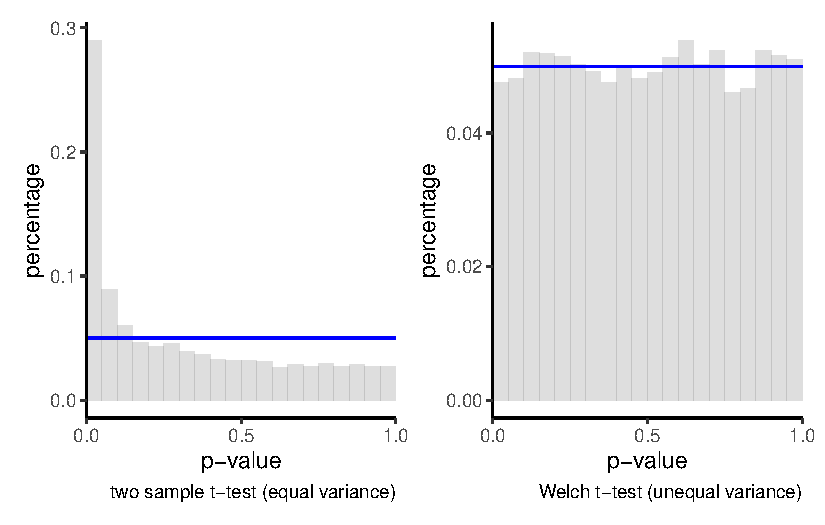
\includegraphics{03-completely_randomized_trials_files/figure-pdf/fig-simuWelchnull-1.pdf}

}

\caption{\label{fig-simuWelchnull}Histogram of the null distribution of
\(p\)-values obtained through simulation using the classical analysis of
variance \(F\)-test (left) and Welch's unequal variance alternative
(right), based on 10 000 simulations. Each simulated sample consist of
50 observations from a \(\mathsf{Normal}(0, 1)\) distribution and 10
observations from \(\mathsf{Normal}(0, 9)\). The uniform distribution
would have 5\% in each of the 20 bins used for the display.}

\end{figure}

We consider for simplicity a problem with \(K=2\) groups, which is the
two-sample \(t\)-test. We simulated 50 observations from a
\(\mathsf{Normal}(0, 1)\) distribution and 10 observations from
\(\mathsf{Normal}(0, 9)\), comparing the distribution of the
\(p\)-values for the Welch and the \(F\)-test statistics.
Figure~\ref{fig-simuWelchnull} shows the results. The percentage of
\(p\)-values less than \(\alpha=0.05\) based on 10 000 replicates is
estimated to be 4.76\% for the Welch statistic, not far from the level.
By contrast, we reject 28.95\% of the time with the one-way ANOVA global
\(F\)-test: this is a large share of innocents sentenced to jail based
on false premises! While the size distortion is not always as striking,
heterogeneity should be accounted in the design by requiring sufficient
sample sizes (whenever costs permits) in each group to be able to
estimate the variance reliably and using an adequate statistic.

\end{example}

There are alternative graphical ways of checking the assumption of equal
variance, many including the standardized residuals
\(r_{ik} = (y_{ik} - \widehat{\mu}_k)/\widehat{\sigma}\) against the
fitted values \(\widehat{\mu}_k\). We will cover these in later
sections.

Oftentimes, unequal variance occurs because the model is not additive.
You could use variance-stabilizing transformations (e.g., log for
multiplicative effects) to ensure approximately equal variance in each
group. Another option is to use a model that is suitable for the type of
response you have (including count and binary data). Lastly, it may be
necessary to explicitly model the variance in more complex design
(including repeated measures) where there is a learning effect over time
and variability decreases as a result. Consult an expert if needed.

\hypertarget{normality}{%
\subsection{Normality}\label{normality}}

There is a persistent yet incorrect claim in the literature that the
data (either response, explanatory or both) must be normal in order to
use (so-called parametric) models like the one-way analysis of variance.
With normal data and equal variances, the eponymous distributions of the
\(F\) and \(t\) tests are exact: knowing the exact distribution does no
harm and is convenient for mathematical derivations. However, it should
be stressed that this condition is \textbf{unnecessary}: the results
hold approximately for large samples by virtue of the central limit
theorem. This probability results dictates that, under general
conditions nearly universally met, the sample mean behaves like a normal
distribution in large samples. This
\href{http://195.134.76.37/applets/AppletCentralLimit/Appl_CentralLimit2.html}{applet}
lets you explore the impact of the underlying population from which the
data are drawn and the interplay with the sample size before the central
limit theorem kicks in. You can view this in
Figure~\ref{fig-Fdistpermut}, where the simulated and theoretical
large-sample distributions are undistinguishable with approximately 20
observations per group.

While many authors may advocate rules of thumbs (sample size of \(n>20\)
or \(n>30\) per group, say), these rules are arbitrary: the
approximation is not much worst at \(n=19\) than at \(n=20\). How large
must the sample size be for the approximation to hold? It largely
depends on the distribution in the population: the more extremes,
skewness, etc. you have, the larger the number of observation must be in
order for the approximation to be valid. Figure~\ref{fig-clt} shows a
skewed to the right bimodal distribution and the distribution of the
sample mean under repeated sampling. Even with \(n=5\) observations
(bottom left), the approximation is not bad but it may still be very far
off with \(n=50\) for heavy-tailed data.

\begin{figure}[ht!]

{\centering 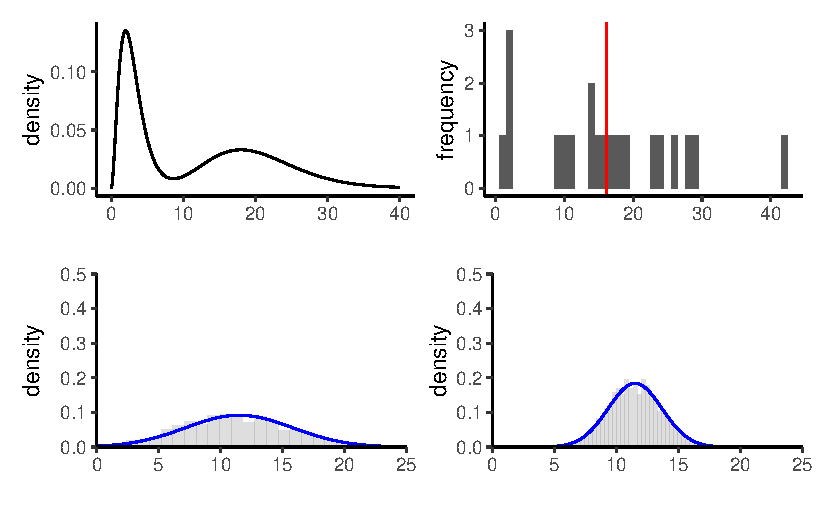
\includegraphics{03-completely_randomized_trials_files/figure-pdf/fig-clt-1.pdf}

}

\caption{\label{fig-clt}Graphical representation of the central limit
theorem. Top left: density of the underlying population from which
samples are drawn. Top right: a sample of 20 observations with its
sample mean (vertical red). Bottom panels: histogram of sample averages
for samples of size 5 (left) and 20 (right) with normal approximation
superimposed. As the sample size increases, the normal approximation for
the mean is more accurate and the standard error decreases.}

\end{figure}

It is important to keep in mind that all statistical statements are
typically approximate and their reliability depends on the sample size:
too small a sample may hampers the strength of your conclusions. The
default graphic for checking whether a sample matches a postulated
distribution is the quantile-quantile plot.

\hypertarget{sec-modelassumptionsindependence}{%
\subsection{Independence}\label{sec-modelassumptionsindependence}}

While I am not allowed to talk of independence as a Quebecer\footnote{All
  credits for this pun are due to C. Genest}, this simply means that
knowing the value of one observation tells us nothing about the value of
any other in the sample. Independence may fail to hold in case of group
structure (family dyads, cluster sampling) which have common
characteristics or more simply in the case of repeated measurements.
Random assignment to treatment is thus key to ensure that the measure
holds, and ensuring at the measurement phase that there is no spillover.

\begin{example}[Independence of
measurements]\protect\hypertarget{exm-measurementindep}{}\label{exm-measurementindep}

There are many hidden ways in which measurements can impact the
response. Physical devices that need to be calibrated before use
(scales, microscope) require tuning: if measurements are done by
different experimenters or on different days, it may impact and add
systematic shift in means for the whole batch.

\end{example}

What is the impact of dependence between measurements? Heuristically,
correlated measurements carry less information than independent ones. In
the most extreme case, there is no additional information and
measurements are identical, but adding them multiple times unduly
inflates the statistic and leads to more frequent rejections.

\begin{figure}[ht!]

{\centering 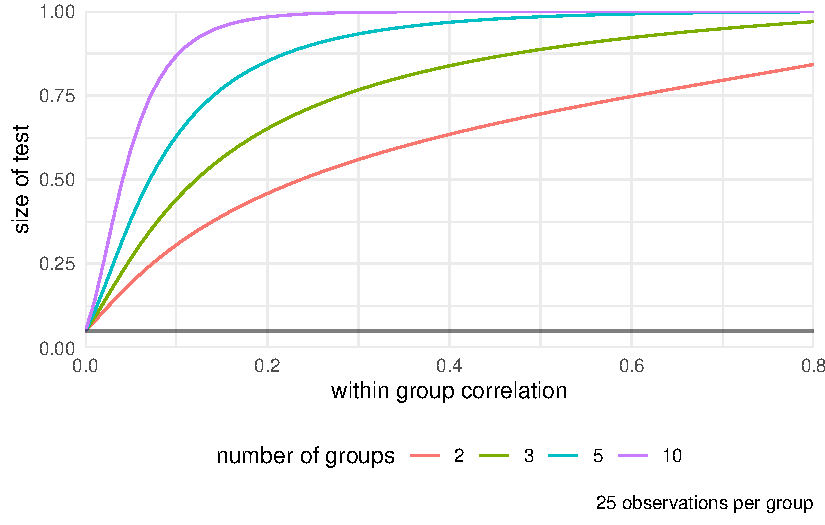
\includegraphics{03-completely_randomized_trials_files/figure-pdf/fig-plotLevelIndep-1.pdf}

}

\caption{\label{fig-plotLevelIndep}Percentage of rejection of the null
hypothesis for the \(F\)-test of equality of means for the one way ANOVA
with data generated with equal mean and variance from an equicorrelation
model (within group observations are correlated, between group
observations are independent). The nominal level of the test is 5\%.}

\end{figure}

The lack of independence can also have drastic consequences on inference
and lead to false conclusions: Figure~\ref{fig-plotLevelIndep} shows an
example with correlated samples within group (or equivalently repeated
measurements from individuals) with 25 observations per group. The
\(y\)-axis shows the proportion of times the null is rejected when it
shouldn't be. Here, since the data are generated from the null model
(equal mean) with equal variance, the inflation in the number of
spurious discoveries, false alarm or type I error is alarming and the
inflation is substantial even with very limited correlation between
measurements.

\bookmarksetup{startatroot}

\hypertarget{contrasts-multiple-testing}{%
\chapter{Contrasts and multiple
testing}\label{contrasts-multiple-testing}}

\begin{tcolorbox}[enhanced jigsaw, colback=white, coltitle=black, rightrule=.15mm, left=2mm, bottomrule=.15mm, toprule=.15mm, titlerule=0mm, colframe=quarto-callout-important-color-frame, leftrule=.75mm, title=\textcolor{quarto-callout-important-color}{\faExclamation}\hspace{0.5em}{Key concept}, breakable, arc=.35mm, colbacktitle=quarto-callout-important-color!10!white, opacitybacktitle=0.6, opacityback=0, toptitle=1mm, bottomtitle=1mm]

\textbf{Learning objectives}:

\begin{itemize}
\tightlist
\item
  Specifying contrast weights to test for differences between groups
\item
  Understanding the problem of multiple testing and the danger for
  selective reporting
\item
  Adjusting for multiple testing to control the global error rate.
\end{itemize}

\end{tcolorbox}

\hypertarget{contrasts}{%
\section{Contrasts}\label{contrasts}}

Suppose we perform an analysis of variance and the \(F\)-test for the
(global) null hypothesis that the averages of all groups are equal is
very large: we reject the null hypothesis in favor of the alternative,
which states that at least one of the group average is different. The
follow-up question will be where these differences lie. Indeed, in an
experimental context, this implies one or more of the manipulation has a
different effect from the others on the mean response. Oftentimes, this
isn't interesting in itself: we could be interested in comparing
different options relative to a \emph{status quo} (e.g., for new drugs
or medical treatment), or determine whether specific combinations work
better than separately, or find the best treatment by comparing all
pairs.

The scientific question of interest that warranted the experiment may
lead to a specific set of hypotheses, which can be formulated by
researchers as comparisons between means of different subgroups. We can
normally express these as \textbf{contrasts}. As
\href{https://stat.ethz.ch/~meier}{Dr.~Lukas Meier} puts it, if the
global \(F\)-test for equality of means is equivalent to a dimly lit
room, contrasts are akin to spotlight that let one focus on particular
aspects of differences in treatments.

Formally speaking, a contrast is a linear combination of averages: in
plain English, this means we assign a weight to each group average and
add them up, and then compare that summary to a postulated value \(a\),
typically zero. Contrasts encode research question of interest: if
\(c_i\) denotes the weight of group average \(\mu_i\)
\((i=1, \ldots, K)\), then we can write the contrast as
\(C = c_1 \mu_1 + \cdots + c_K \mu_K\) with the null hypothesis
\(\mathscr{H}_0: C=a\) for a two-sided alternative. The sample estimate
of the linear contrast is obtained by replacing the unknown population
average \(\mu_i\) by the sample average of that group,
\(\widehat{\mu}_i = \overline{y}_{i}\). We can easily obtain the
standard error of the linear combination \(C.\)\footnote{Should you ever
  need the formula, the standard error assuming subsample size of
  \(n_1, \ldots, n_K\) and a common variance \(\sigma^2\) is
  \(\sqrt{\mathsf{Va}(\widehat{C})}\), where
  \[\mathsf{Va}(\widehat{C}) = \widehat{\sigma}^2\left(\frac{c_1^2}{n_1} + \cdots + \frac{c_K^2}{n_K}\right).\]}
We can then build a \(t\) statistic as usual by looking at the
difference between our postulated value and the observed weighted mean,
suitably standardized. If the global \(F\)-test leads to rejection of
the null, there exists a contrast which is significant at the same
level.

\hypertarget{orthogonal-contrasts}{%
\subsection{Orthogonal contrasts}\label{orthogonal-contrasts}}

Sometimes, linear contrasts encode disjoint bits of information about
the sample: for example, one contrast that compares groups the first two
groups versus one that compares the third and fourth is in effect using
data from two disjoint samples, as contrasts are based on sample
averages. Whenever the contrasts vectors are orthogonal, the tests will
be uncorrelated. Mathematically, if we let \(c_{i}\) and \(c^{*}_{i}\)
denote weights attached to the mean of group \(i\) comprising \(n_i\)
observations, contrasts are orthogonal if
\(c_{1}c^{*}_{1}/n_1 + \cdots + c_{K}c^{*}_K/n_K = 0\); if the sample is
balanced with the same number of observations in each group,
\(n/K = n_1 =\cdots = n_K\), we can consider the dot product of the two
contrast vectors and neglect the subsample sizes.

If we have \(K\) groups, there are \(K-1\) contrasts for pairwise
differences, the last one being captured by the sample mean for the
overall effect\footnote{The constraint \(c_1 + \cdots + c_K=0\) ensures
  that linear contrasts are orthogonal to the mean, which has weight
  \(c_i=n_i/n\) and for balanced samples \(c_i =1/n\).}. If we care only
about difference between groups (as opposed to the overall effect of all
treatments), we impose a sum-to-zero constraint on the weights so
\(c_1 + \cdots + c_K=0\). Keep in mind that, although independent tests
are nice mathematically, contrasts should encode the hypothesis of
interest to the researchers: we choose contrasts because they are
meaningful, not because they are orthogonal.

\begin{example}[Contrasts for encouragement on
teaching]\protect\hypertarget{exm-contrast-teaching}{}\label{exm-contrast-teaching}

The \texttt{arithmetic} data example considered five different treatment
groups with 9 individuals in each. Two of them were control groups, one
received praise, another was reproved and the last was ignored.

Suppose that researchers were interested in assessing whether the
experimental manipulation had an effect, and whether the impact of
positive and negative feedback is the same on students.\footnote{These
  would be formulated \emph{at registration time}, but for the sake of
  the argument we proceed as if they were.}

Suppose we have five groups in the order (control 1, control 2, praised,
reproved, ignored). We can express these hypothesis as

\begin{itemize}
\tightlist
\item
  \(\mathscr{H}_{01}\): \(\mu_{\text{praise}} = \mu_{\text{reproved}}\)
\item
  \(\mathscr{H}_{02}\): \begin{align*}
  \frac{1}{2}(\mu_{\text{control}_1}+\mu_{\text{control}_2}) = \frac{1}{3}\mu_{\text{praised}} + \frac{1}{3}\mu_{\text{reproved}} + \frac{1}{3}\mu_{\text{ignored}}
  \end{align*}
\end{itemize}

Note that, for the hypothesis of control vs experimental manipulation,
we look at average of the different groups associated with each item.
Using the ordering, the weights of the contrast vector are
\((1/2, 1/2, -1/3, -1/3, -1/3)\) and \((0, 0, 1, -1, 0)\). There are
many equivalent formulation: we could multiply the weights by any number
(different from zero) and we would get the same test statistic, as the
latter is standardized.

\begin{Shaded}
\begin{Highlighting}[]
\FunctionTok{library}\NormalTok{(emmeans)}
\FunctionTok{data}\NormalTok{(arithmetic, }\AttributeTok{package =} \StringTok{"hecedsm"}\NormalTok{)}
\NormalTok{linmod }\OtherTok{\textless{}{-}} \FunctionTok{aov}\NormalTok{(score }\SpecialCharTok{\textasciitilde{}}\NormalTok{ group, }\AttributeTok{data =}\NormalTok{ arithmetic)}
\NormalTok{linmod\_emm }\OtherTok{\textless{}{-}} \FunctionTok{emmeans}\NormalTok{(linmod, }\AttributeTok{specs =} \StringTok{\textquotesingle{}group\textquotesingle{}}\NormalTok{)}
\NormalTok{contrast\_specif }\OtherTok{\textless{}{-}} \FunctionTok{list}\NormalTok{(}
  \AttributeTok{controlvsmanip =} \FunctionTok{c}\NormalTok{(}\FloatTok{0.5}\NormalTok{, }\FloatTok{0.5}\NormalTok{, }\SpecialCharTok{{-}}\DecValTok{1}\SpecialCharTok{/}\DecValTok{3}\NormalTok{, }\SpecialCharTok{{-}}\DecValTok{1}\SpecialCharTok{/}\DecValTok{3}\NormalTok{, }\SpecialCharTok{{-}}\DecValTok{1}\SpecialCharTok{/}\DecValTok{3}\NormalTok{),}
  \AttributeTok{praisedvsreproved =} \FunctionTok{c}\NormalTok{(}\DecValTok{0}\NormalTok{, }\DecValTok{0}\NormalTok{, }\DecValTok{1}\NormalTok{, }\SpecialCharTok{{-}}\DecValTok{1}\NormalTok{, }\DecValTok{0}\NormalTok{)}
\NormalTok{)}
\NormalTok{contrasts\_res }\OtherTok{\textless{}{-}} 
  \FunctionTok{contrast}\NormalTok{(}\AttributeTok{object =}\NormalTok{ linmod\_emm, }
                    \AttributeTok{method =}\NormalTok{ contrast\_specif)}
\CommentTok{\# Obtain confidence intervals instead of p{-}values}
\FunctionTok{confint}\NormalTok{(contrasts\_res)}
\end{Highlighting}
\end{Shaded}

\hypertarget{tbl-contrast-arithmetic-confint}{}
\begin{table}
\caption{\label{tbl-contrast-arithmetic-confint}Contrasts estimates for the arithmetic data }\tabularnewline

\centering
\begin{tabular}{lrrrrr}
\toprule
contrast & estimate & std. error & df & lower (CI) & upper (conf. limit)CI)\\
\midrule
control vs manip & -3.33 & 1.05 & 40 & -5.45 & -1.22\\
praised vs reproved & 4.00 & 1.62 & 40 & 0.72 & 7.28\\
\bottomrule
\end{tabular}
\end{table}

\end{example}

\begin{example}[Teaching to
read]\protect\hypertarget{exm-teachingtoread}{}\label{exm-teachingtoread}

We consider data from Baumann, Seifert-Kessell, and Jones (1992). The
abstract of the paper provides a brief description of the study

\begin{quote}
This study investigated the effectiveness of explicit instruction in
think aloud as a means to promote elementary students' comprehension
monitoring abilities. Sixty-six fourth-grade students were randomly
assigned to one of three experimental groups: (a) a Think-Aloud (TA)
group, in which students were taught various comprehension monitoring
strategies for reading stories (e.g., self-questioning, prediction,
retelling, rereading) through the medium of thinking aloud; (b) a
Directed reading-Thinking Activity (DRTA) group, in which students were
taught a predict-verify strategy for reading and responding to stories;
or (c) a Directed reading Activity (DRA) group, an instructed control,
in which students engaged in a noninteractive, guided reading of
stories.
\end{quote}

Looking at Table~\ref{tbl-print-pairwise-baumann}, we can see that
\texttt{DRTA} has the highest average, followed by \texttt{TA} and
directed reading (\texttt{DR}).

\begin{Shaded}
\begin{Highlighting}[]
\FunctionTok{library}\NormalTok{(emmeans) }\CommentTok{\#load package}
\FunctionTok{data}\NormalTok{(BSJ92, }\AttributeTok{package =} \StringTok{"hecedsm"}\NormalTok{)}
\NormalTok{mod\_post }\OtherTok{\textless{}{-}} \FunctionTok{aov}\NormalTok{(posttest1 }\SpecialCharTok{\textasciitilde{}}\NormalTok{ group, }\AttributeTok{data =}\NormalTok{ BSJ92)}
\NormalTok{emmeans\_post }\OtherTok{\textless{}{-}} \FunctionTok{emmeans}\NormalTok{(}\AttributeTok{object =}\NormalTok{ mod\_post, }
                        \AttributeTok{specs =} \StringTok{"group"}\NormalTok{)}
\end{Highlighting}
\end{Shaded}

\hypertarget{tbl-print-pairwise-baumann}{}
\begin{table}
\caption{\label{tbl-print-pairwise-baumann}Estimated group averages with standard errors and 95\% confidence
intervals for post-test 1. }\tabularnewline

\centering
\begin{tabular}{lrrrrr}
\toprule
terms & marg. mean & std. err. & dof & lower (CI) & upper (CI)\\
\midrule
DR & 6.68 & 0.68 & 63 & 5.32 & 8.04\\
DRTA & 9.77 & 0.68 & 63 & 8.41 & 11.13\\
TA & 7.77 & 0.68 & 63 & 6.41 & 9.13\\
\bottomrule
\end{tabular}
\end{table}

The purpose of Baumann, Seifert-Kessell, and Jones (1992) was to make a
particular comparison between treatment groups. From the abstract:

\begin{quote}
The primary quantitative analyses involved two planned orthogonal
contrasts---effect of instruction (TA + DRTA vs.~2 x DRA) and intensity
of instruction (TA vs.~DRTA)---for three whole-sample dependent
measures: (a) an error detection test, (b) a comprehension monitoring
questionnaire, and (c) a modified cloze test.
\end{quote}

The hypothesis of Baumann, Seifert-Kessell, and Jones (1992) is
\(\mathscr{H}_0: \mu_{\mathrm{TA}} + \mu_{\mathrm{DRTA}} = 2 \mu_{\mathrm{DRA}}\)
or, rewritten slightly, \begin{align*}
\mathscr{H}_0: - 2 \mu_{\mathrm{DR}} + \mu_{\mathrm{DRTA}} + \mu_{\mathrm{TA}} = 0.
\end{align*} with weights \((-2, 1, 1)\); the order of the levels for
the treatment are (\(\mathrm{DRA}\), \(\mathrm{DRTA}\), \(\mathrm{TA}\))
and it must match that of the coefficients. An equivalent formulation is
\((2, -1, -1)\) or \((1, -1/2, -1/2)\): in either case, the estimated
differences will be different (up to a constant multiple or a sign
change). The vector of weights for
\(\mathscr{H}_0: \mu_{\mathrm{TA}} = \mu_{\mathrm{DRTA}}\) is (\(0\),
\(-1\), \(1\)): the zero appears because the first component,
\(\mathrm{DRA}\) doesn't appear. The two contrasts are orthogonal since
\((-2 \times 0) + (1 \times -1) + (1 \times 1) = 0\).

\begin{Shaded}
\begin{Highlighting}[]
\CommentTok{\# Identify the order of the level of the variables}
\FunctionTok{with}\NormalTok{(BSJ92, }\FunctionTok{levels}\NormalTok{(group))}
\end{Highlighting}
\end{Shaded}

\begin{verbatim}
[1] "DR"   "DRTA" "TA"  
\end{verbatim}

\begin{Shaded}
\begin{Highlighting}[]
\CommentTok{\# DR, DRTA, TA (alphabetical)}
\NormalTok{contrasts\_list }\OtherTok{\textless{}{-}} \FunctionTok{list}\NormalTok{(}
  \StringTok{"C1: DRTA+TA vs 2DR"} \OtherTok{=} \FunctionTok{c}\NormalTok{(}\SpecialCharTok{{-}}\DecValTok{2}\NormalTok{, }\DecValTok{1}\NormalTok{, }\DecValTok{1}\NormalTok{), }
  \CommentTok{\# Contrasts: linear combination of means, coefficients sum to zero}
  \CommentTok{\# 2xDR = DRTA + TA =\textgreater{} {-}2*DR + 1*DRTA + 1*TA = 0 and {-}2+1+1 = 0}
  \StringTok{"C1: average (DRTA+TA) vs DR"} \OtherTok{=} \FunctionTok{c}\NormalTok{(}\SpecialCharTok{{-}}\DecValTok{1}\NormalTok{, }\FloatTok{0.5}\NormalTok{, }\FloatTok{0.5}\NormalTok{), }
  \CommentTok{\#same thing, but halved so in terms of average}
  \StringTok{"C2: DRTA vs TA"} \OtherTok{=} \FunctionTok{c}\NormalTok{(}\DecValTok{0}\NormalTok{, }\DecValTok{1}\NormalTok{, }\SpecialCharTok{{-}}\DecValTok{1}\NormalTok{),}
  \StringTok{"C2: TA vs DRTA"} \OtherTok{=} \FunctionTok{c}\NormalTok{(}\DecValTok{0}\NormalTok{, }\SpecialCharTok{{-}}\DecValTok{1}\NormalTok{, }\DecValTok{1}\NormalTok{) }
  \CommentTok{\# same, but sign flipped}
\NormalTok{)}
\NormalTok{contrasts\_post }\OtherTok{\textless{}{-}} 
  \FunctionTok{contrast}\NormalTok{(}\AttributeTok{object =}\NormalTok{ emmeans\_post,}
           \AttributeTok{method =}\NormalTok{ contrasts\_list)}
\NormalTok{contrasts\_summary\_post }\OtherTok{\textless{}{-}} \FunctionTok{summary}\NormalTok{(contrasts\_post)}
\end{Highlighting}
\end{Shaded}

\hypertarget{tbl-print-contrasts}{}
\begin{table}
\caption{\label{tbl-print-contrasts}Estimated contrasts for post-test 1. }\tabularnewline

\centering
\begin{tabular}{lrrrrr}
\toprule
contrast & estimate & std. err. & dof & stat & p-value\\
\midrule
C1: DRTA+TA vs 2DR & 4.18 & 1.67 & 63 & 2.51 & 0.01\\
C1: average (DRTA+TA) vs DR & 2.09 & 0.83 & 63 & 2.51 & 0.01\\
C2: DRTA vs TA & 2.00 & 0.96 & 63 & 2.08 & 0.04\\
C2: TA vs DRTA & -2.00 & 0.96 & 63 & -2.08 & 0.04\\
\bottomrule
\end{tabular}
\end{table}

We can look at these differences; since \texttt{DRTA} versus \texttt{TA}
is a pairwise difference, we could have obtained the \(t\)-statistic
directly from the pairwise contrasts using
\texttt{pairs(emmeans\_post)}. Note that the two different ways of
writing the comparison between \texttt{DR} and the average of the other
two methods yield different point estimates, but same inference (i.e.,
the same \(p\)-values). For contrast \(C_{1b}\), we get half the
estimate (but the standard error is also halved) and likewise for the
second contrasts we get an estimate of
\(\mu_{\mathrm{DRTA}} - \mu_{\mathrm{TA}}\) in the first case (\(C_2\))
and \(\mu_{\mathrm{TA}} - \mu_{\mathrm{DRTA}}\): the difference in group
averages is the same up to sign.

What is the conclusion of our analysis of contrasts? It looks like the
methods involving teaching aloud have a strong impact on reading
comprehension relative to only directed reading. The evidence is not as
strong when we compare the method that combines directed
reading-thinking activity and thinking aloud.

\end{example}

\begin{example}[Paper or
plastic]\protect\hypertarget{exm-paperorplastic}{}\label{exm-paperorplastic}

Sokolova, Krishna, and Döring (2023) consider consumer bias when
assessing how eco-friendly packages are. Items such as cereal are
packaged in plastic bags, which themselves are covered in a box. They
conjecture (and find) that consumers tend to view the packaging as being
more eco-friendly when the amount of cardboard or paper surrounding the
box is large, relative to the sole plastic package. We consider the data
Study 2A, which measures the perceived environmental friendliness (PEF)
as a function of the proportion of paper wrapping (either none, half of
the area of the plastic, equal or twice). The authors are interested in
comparing none with other choices.

If \(\mu_{0}, \mu_{0.5}, \mu_{1}, \mu_2\) denote the true mean of the
PEF score as a function of the proportion of paper, we are interested in
pairwise differences, but only relative to the reference \(\mu_{0}\):
\begin{align*}
\mu_0 = \mu_{0.5}  & \iff 1\mu_0 - 1\mu_{0.5} + 0\mu_{1} + 0 \mu_{2} = 0\\
\mu_0 = \mu_{1} & \iff 1\mu_0 + 0\mu_{0.5} -1\mu_{1} + 0 \mu_{2} = 0\\
\mu_0 = \mu_{2} & \iff 1\mu_0 + 0\mu_{0.5} + 0\mu_{1} -1 \mu_{2} = 0
\end{align*} so contrast vectors \((1, -1, 0, 0)\), \((1, 0, -1, 0)\)
and \((1, 0, 0, -1)\) would allow one to test the hypothesis.

\begin{Shaded}
\begin{Highlighting}[]
\FunctionTok{data}\NormalTok{(SKD23\_S2A, }\AttributeTok{package =} \StringTok{"hecedsm"}\NormalTok{) }\CommentTok{\# load data}
\NormalTok{linmod }\OtherTok{\textless{}{-}} \FunctionTok{lm}\NormalTok{(pef }\SpecialCharTok{\textasciitilde{}}\NormalTok{ proportion, }\AttributeTok{data =}\NormalTok{ SKD23\_S2A) }\CommentTok{\# fit simple linear regression}
\FunctionTok{anova}\NormalTok{(linmod) }\CommentTok{\# check for significance of slope}
\FunctionTok{coef}\NormalTok{(linmod) }\CommentTok{\# extract intercept and slope}
\NormalTok{anovamod }\OtherTok{\textless{}{-}} \FunctionTok{lm}\NormalTok{(pef }\SpecialCharTok{\textasciitilde{}} \FunctionTok{factor}\NormalTok{(proportion), }\AttributeTok{data =}\NormalTok{ SKD23\_S2A) }\CommentTok{\# one{-}way ANOVA}
\NormalTok{margmean }\OtherTok{\textless{}{-}}\NormalTok{ anovamod }\SpecialCharTok{|\textgreater{}}\NormalTok{  emmeans}\SpecialCharTok{::}\FunctionTok{emmeans}\NormalTok{(}\AttributeTok{specs =} \StringTok{"proportion"}\NormalTok{) }\CommentTok{\# group means}
\NormalTok{contrastlist }\OtherTok{\textless{}{-}} \FunctionTok{list}\NormalTok{( }\CommentTok{\# specify contrast vectors}
   \AttributeTok{refvshalf =} \FunctionTok{c}\NormalTok{(}\DecValTok{1}\NormalTok{, }\SpecialCharTok{{-}}\DecValTok{1}\NormalTok{, }\DecValTok{0}\NormalTok{, }\DecValTok{0}\NormalTok{),}
   \AttributeTok{refvsone =}  \FunctionTok{c}\NormalTok{(}\DecValTok{1}\NormalTok{, }\DecValTok{0}\NormalTok{, }\SpecialCharTok{{-}}\DecValTok{1}\NormalTok{, }\DecValTok{0}\NormalTok{),}
   \AttributeTok{refvstwo =}  \FunctionTok{c}\NormalTok{(}\DecValTok{1}\NormalTok{, }\DecValTok{0}\NormalTok{, }\DecValTok{0}\NormalTok{, }\SpecialCharTok{{-}}\DecValTok{1}\NormalTok{))}
\CommentTok{\# compute contrasts relative to reference }
\NormalTok{margmean }\SpecialCharTok{|\textgreater{}}\NormalTok{ emmeans}\SpecialCharTok{::}\FunctionTok{contrast}\NormalTok{(}\AttributeTok{method =}\NormalTok{ contrastlist)}
\end{Highlighting}
\end{Shaded}

The group averages are reported in Table~\ref{tbl-print-groupmeans-PEF},
match those reported by the authors in the paper. They suggest an
increased perceived environmental friendliness as the amount of paper
used in the wrapping increases. We could fit a simple regression model
to assess the average change, treating the proportion as a continuous
explanatory variable. The estimated slope for the change in PEF score,
which ranges from 1 to 7 in increments of 0.25, is 0.53 per area of
paper. There is however strong evidence, given the data, that the change
isn't quite linear, as the fit of the linear regression model is
significantly worse than the corresponding linear model.

\hypertarget{tbl-print-groupmeans-PEF}{}
\begin{table}
\caption{\label{tbl-print-groupmeans-PEF}Estimated group averages of PEF per proportion with standard errors }\tabularnewline

\centering
\begin{tabular}{rrrrrr}
\toprule
proportion & marg. mean & std. err. & dof & lower (CI) & upper (CI)\\
\midrule
0.0 & 2.16 & 0.093 & 798 & 1.98 & 2.34\\
0.5 & 2.91 & 0.093 & 798 & 2.73 & 3.09\\
1.0 & 3.06 & 0.092 & 798 & 2.88 & 3.24\\
2.0 & 3.34 & 0.089 & 798 & 3.17 & 3.52\\
\bottomrule
\end{tabular}
\end{table}

\hypertarget{tbl-print-contrast-PEF}{}
\begin{table}
\caption{\label{tbl-print-contrast-PEF}Estimated contrasts for differences of PEF to no paper. }\tabularnewline

\centering
\begin{tabular}{lrrrrr}
\toprule
contrast & estimate & std. err. & dof & stat & p-value\\
\midrule
refvshalf & -0.75 & 0.13 & 798 & -5.71 & 0\\
refvsone & -0.90 & 0.13 & 798 & -6.89 & 0\\
refvstwo & -1.18 & 0.13 & 798 & -9.20 & 0\\
\bottomrule
\end{tabular}
\end{table}

All differences reported in Table~\ref{tbl-print-contrast-PEF} are
significant and positive, in line with the researcher's hypothesis.

\end{example}

\hypertarget{multiple-testing}{%
\section{Multiple testing}\label{multiple-testing}}

Beyond looking at the global null, we will be interested in a set of
contrast statistics and typically this number can be large-ish. There is
however a catch in starting to test multiple hypothesis at once.

If you do a \textbf{single} hypothesis test and the testing procedure is
well calibrated (meaning that the model model assumptions hold),
\(p\)-values are generated uniformly on the interval \([0,1]\) and there
is a probability of \(\alpha\) of making a type I error (i.e.,
concluding in favour of the alternative and rejecting the null
incorrectly) if the null is true. The problem of the above approach is
that the more tests you perform, the higher the chance of finding
(incorrectly) something: with 20 independent tests, we expect that, on
average, one of them will yield a \(p\)-value less than 5\% even if this
is a fluke. The problem with multiple testing is not so much that it
occurs, but more than researchers tend to report selectively findings
and only give the results of tests for which \(p \leq \alpha\), even if
these are typically the product of chance. This makes most findings will
not replicate: if we rerun the experiment, we will typically not find
the same result.

There is an infinite potential number of contrasts with more than two
factos. Not all tests are of interest: standard software will report all
possible pairwise comparisons, but this may not be of interest as
showcased in Example~\ref{exm-paperorplastic}. If there are \(K\) groups
to compare and any comparison is of interest, than we could performs
\(\binom{K}{2}\) pairwise comparisons with
\(\mathscr{H}_{0}: \mu_i = \mu_j\) for \(i \neq j\). For \(K=3\), there
are three such comparisons, 10 pairwise comparisons if \(K=5\) and 45
pairwise comparisons if \(K=10\). The number of pairwise comparisons
grows quickly.

The number of tests performed in the course of an analysis can be very
large. Y. Benjamini investigated the number of tests performed in each
study of the Psychology replication project (Nosek et al. 2015): this
number ranged from 4 to 700, with an average of 72 --- most studies did
not account for the fact they were performing multiple tests or selected
the model and thus some `discoveries' are bound to be spurious. It is
natural to ask then how many results are spurious findings that
correspond to type I errors. The paramount (absurd) illustration is the
cartoon presented in Figure~\ref{fig-xkcdsignificant}: note how there is
little scientific backing for the theory (thus such test shouldn't be of
interest to begin with) and likewise the selective reporting made of the
conclusions, despite nuanced conclusions.

We can also assess mathematically the problem. Assume for simplicity
that all tests are independent\footnote{This is the case if tests are
  based on different data, or if the contrasts considered are orthogonal
  under normality.}, then the probability of any rejecting the null
incorrectly is \(\alpha\), but larger over the collection (with tests
\(A\) and \(B\), we could reject by mistake if \(A\) is a type I error
and \(B\) isn't, or vice-versa, or if both are incorrect rejections.

The probability of making at least one type I error if each test is
conducted at level \(\alpha\), say \(\alpha^{\star}\), is\footnote{The
  second line holds with independent observations, the second follows
  from the use of Boole's inequality and does not require independent
  tests.} \begin{align}
\alpha^{\star} &= 1 - \text{probability of making no type I error} 
\\ &= 1- (1-\alpha)^m
\\ & \leq m\alpha
\end{align}

With \(\alpha = 5\)\% and \(m=4\) tests,
\(\alpha^{\star} \approx 0.185\) whereas for \(m=72\) tests,
\(\alpha^{\star} \approx 0.975\): this means we are almost guaranteed
even when nothing is going on to find ``statistically significant'' yet
meaningless results.

\begin{figure}[ht!]

{\centering 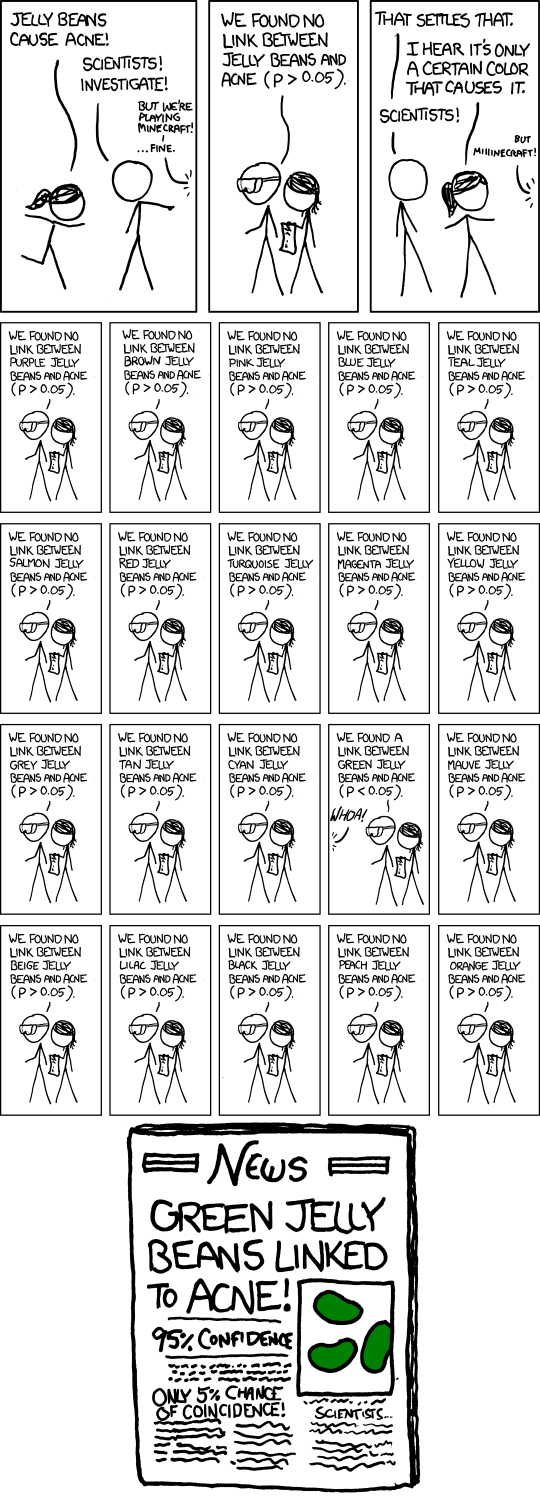
\includegraphics[width=1.8in,height=\textheight]{figures/xkcd882_significant.png}

}

\caption{\label{fig-xkcdsignificant}xkcd 882: Significant. The alt text
is `So, uh, we did the green study again and got no link. It was
probably a--' `RESEARCH CONFLICTED ON GREEN JELLY BEAN/ACNE LINK; MORE
STUDY RECOMMENDED!'}

\end{figure}

It is sensible to try and reduce or bound the number of false positive
or control the probability of getting spurious findings. We consider a
\textbf{family} of \(m\) null hypothesis
\(\mathscr{H}_{01}, \ldots, \mathscr{H}_{0m}\), i.e.~a collection of
\(m\) hypothesis tests. The exact set depends on the context, but this
comprises all hypothesis that are scientifically relevant and could be
reported. These comparisons are called \textbf{pre-planned comparisons}:
they should be chosen before the experiment takes place and
pre-registered to avoid data dredging and selective reporting. The
number of planned comparisons should be kept small relative to the
number of parameters: for a one-way ANOVA, a general rule of thumb is to
make no more comparisons than the number of groups, \(K\).

Suppose that we perform \(m\) hypothesis tests in a study and define
binary indicators \begin{align}
R_i &= \begin{cases} 1 & \text{if we reject the null hypothesis }  \mathscr{H}_{0i} \\
0 & \text{if we fail to reject } \mathscr{H}_{0i}
\end{cases}\\
V_i &=\begin{cases} 1 & \text{type I error for } \mathscr{H}_{0i}\quad  (R_i=1 \text{ and  }\mathscr{H}_{0i} \text{ is true}) \\ 0 & \text{otherwise}.
\end{cases}
\end{align} With this notation, \(R=R_1 + \cdots + R_m\) simply encodes
the total number of rejections (\(0 \leq R \leq m\)), and
\(V = V_1 + \cdots + V_m\) is the number of null hypothesis rejected by
mistake (\(0 \leq V \leq R\)).

The \textbf{familywise error rate} is the probability of making at least
one type I error for the whole collection or test, in other words per
family, is \begin{align*}
\mathsf{FWER} = \Pr(V \geq 1).
\end{align*} To control the familywise error rate, one must be more
stringent in rejecting the null and perform each test with a smaller
level \(\alpha\) so that the overall or simultaneous probability is less
than \(\mathsf{FWER}\).

\hypertarget{bonferronis-procedure}{%
\subsection{Bonferroni's procedure}\label{bonferronis-procedure}}

The easiest way to control for multiple testing is to perform each test
at level \(\alpha/m\), thereby ensuring that the family-wise error is
controlled at level \(\alpha\). This is a good option if \(m\) is small
and the Bonferroni adjustment also controls the \textbf{per-family error
rate}, which is the expected (theoretical average) number of false
positive \(\mathsf{PFER} = \mathsf{E}(V)\). The latter is a more
stringent criterion than the familywise error rate because
\(\Pr(V \geq 1) \leq \mathsf{E}(V)\): the familywise error rate does not
make a distinction between having one or multiple type I
errors.\footnote{By definition, the expected number of false positive
  (PFER) is
  \(\mathsf{E}(V) = \sum_{i=1}^m i \Pr(V=i) \geq \sum_{i=1}^m \Pr(V=i) = \Pr(V \geq 1)\),
  so larger than the probability of making at least type 1 error. Thus,
  any procedure that controls the per-family error rate (e.g.,
  Bonferroni) also automatically bounds the familywise error rate.}

Why is Bonferroni's procedure popular? It is conceptually easy to
understand and simple, and it applies to any design and regardless of
the dependence between the tests. However, the number of tests to adjust
for, \(m\), must be prespecified and the procedure leads to low power
when the size of the family is large, meaning it makes detection of
non-null effects more difficult. Moreover, if our sole objective is to
control for the familywise error rate, then there are other procedures
that are always better in the sense that they still control the
\(\mathsf{FWER}\) while leading to increased capacity of detection when
the null is false.

If the raw (i.e., unadjusted) \(p\)-values are reported, we reject
hypothesis \(\mathscr{H}_{0i}\) if \(m \times p_i \ge \alpha\):
operationally, we multiply each \(p\)-value by \(m\) and reject if the
result exceeds \(\alpha\).

\hypertarget{holmbonferronis-procedure}{%
\subsection{Holm--Bonferroni's
procedure}\label{holmbonferronis-procedure}}

The idea of Holm's procedure is to use a sharper inequality bound and
amounts to performing tests at different levels, with more stringent for
smaller \(p\)-values. To perform Holm--Bonferroni,

\begin{enumerate}
\def\labelenumi{\arabic{enumi}.}
\tightlist
\item
  order the \(p\)-values of the family of \(m\) tests from smallest to
  largest, \(p_{(1)} \leq \cdots \leq p_{(m)}\)
\item
  test sequentially the hypotheses: coupling Holm's method with
  Bonferroni's procedure, we compare \(p_{(1)}\) to
  \(\alpha_{(1)} = \alpha/m\), \(p_{(2)}\) to
  \(\alpha_{(2)}=\alpha/(m-1)\), etc. If \(p_{(j)} \geq \alpha_{(j)}\)
  but \(p_{(i)} \leq \alpha_{(i)}\) for \(i=1, \ldots, j-1\) (all
  smaller \(p\)-values), we reject the associated hypothesis
  \(\mathscr{H}_{0(1)}, \ldots, \mathscr{H}_{0(j-1)}\) but fail to
  reject \(\mathscr{H}_{0(j)}, \ldots, \mathscr{H}_{0(m)}\).
\end{enumerate}

If all of the \(p\)-values are less than their respective levels, than
we still reject each null hypothesis. Otherwise, we reject all the tests
whose \(p\)-values exceeds the smallest nonsignificant one. This
procedure doesn't control the per-family error rate, but is uniformly
more powerful (lingo to say that it's universally better for control)
and thus leads to increased detection than Bonferroni's method. To see
this, consider a family of \(m=3\) \(p\)-values with values \(0.01\),
\(0.04\) and \(0.02\). Bonferroni's adjustment would lead us to reject
the second and third hypotheses at level \(\alpha=0.05\), but not
Holm-Bonferroni.

\hypertarget{multiple-testing-methods-for-analysis-of-variance}{%
\subsection{Multiple testing methods for analysis of
variance}\label{multiple-testing-methods-for-analysis-of-variance}}

There are specialized procedures for the analysis of variance problem
that leverages some of the assumptions (equal variance, large sample
approximation for the distribution of means). There are three scenarios

\begin{enumerate}
\def\labelenumi{\arabic{enumi}.}
\tightlist
\item
  Dunnett's method for comparison to a reference or control group,
  controlling only for \(K-1\) pairwise differences
\item
  Tukey's range procedure, also termed \emph{honestly significant
  difference} (HSD), for \textbf{all} pairwise differences. We can
  obtain control on the type I error by looking at what happens between
  the minimum and maximum group averages under the null.
\item
  Scheffe's method for contrasts. This is useful when the number of
  contrasts of interest is not specified apriori.
\end{enumerate}

If the global \(F\)-test does not find differences at level \(\alpha\),
then Scheffe's method will also find no significant contrast \(\alpha\)
but nothing can be said about other methods. Generally, the more tests
we control the type error for, the more conservative the procedures are.

In \textbf{R}, we can use the \texttt{multcomp} or \texttt{emmeans}
packages for the tests to adjust, or compute results manually. The test
statistics do not change, only the benchmark null distribution is
different. Figure~\ref{fig-references-multtest} shows what the
\(p\)-value would be depending on how we control for contrasts. For
reasonable values, we get larger \(p\)-values for the methods that
provide control.

\begin{figure}[ht!]

{\centering 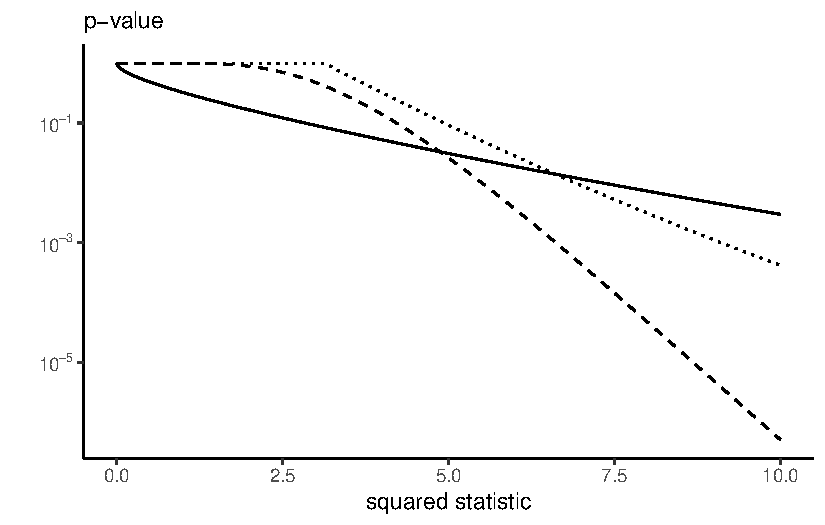
\includegraphics{04-contrasts_multipletesting_files/figure-pdf/fig-references-multtest-1.pdf}

}

\caption{\label{fig-references-multtest}P-value as a function of the
squared t-statistic for a contrast for no adjustment (full line),
Tukey's HSD (dashed line) and Scheffe's adjustment (dotted).}

\end{figure}

\begin{example}[Multiple testing for paper or
plastic]\protect\hypertarget{exm-paperorplastic}{}\label{exm-paperorplastic}

Sokolova, Krishna, and Döring (2023) considered pairwise difference
relative to the control where only plastic wrapping is used. We could
use either Bonferroni, Holm--Bonferoni or Dunnett's method. Since the
\(p\)-values are tiny (less than \(10^{-4}\)), this has no impact on the
conclusions whatsoever. To better appreciate the impact in small
samples, we subsample 20 observation per group to inflate \(p\)-values.
We can also see differences by inspecting the width of the confidence
intervals for the pairwise differences to the reference group: more
conservative references lead to wider intervals.

\begin{Shaded}
\begin{Highlighting}[]
\FunctionTok{data}\NormalTok{(SKD23\_S2A, }\AttributeTok{package =} \StringTok{"hecedsm"}\NormalTok{) }\CommentTok{\# load data}
\FunctionTok{set.seed}\NormalTok{(}\DecValTok{80667}\NormalTok{) }\CommentTok{\# Set seed for reproducibility}
\NormalTok{SKD23\_S2A\_sub }\OtherTok{\textless{}{-}}\NormalTok{ SKD23\_S2A }\SpecialCharTok{|\textgreater{}}
  \CommentTok{\# Create a categorical variable (factor) and ensure reference is 0}
  \CommentTok{\# By default, it would be (first alphanumerical value of labels)}
\NormalTok{  dplyr}\SpecialCharTok{::}\FunctionTok{mutate}\NormalTok{(}\AttributeTok{propfact =} \FunctionTok{relevel}\NormalTok{(}\FunctionTok{factor}\NormalTok{(proportion), }\AttributeTok{ref =} \StringTok{"0"}\NormalTok{)) }\SpecialCharTok{|\textgreater{}}
  \CommentTok{\# Sample only fourty observations by group {-}}
  \CommentTok{\# for illustration purposes only, otherwise p{-}values are too small}
\NormalTok{  dplyr}\SpecialCharTok{::}\FunctionTok{slice\_sample}\NormalTok{(}\AttributeTok{n =} \DecValTok{20}\NormalTok{, }\AttributeTok{by =}\NormalTok{ propfact)}
\NormalTok{anovamod }\OtherTok{\textless{}{-}} \FunctionTok{lm}\NormalTok{(pef }\SpecialCharTok{\textasciitilde{}}\NormalTok{ propfact, }\AttributeTok{data =}\NormalTok{ SKD23\_S2A\_sub) }
\FunctionTok{library}\NormalTok{(emmeans)}
\NormalTok{margmean }\OtherTok{\textless{}{-}} \FunctionTok{emmeans}\NormalTok{(}
\NormalTok{  anovamod, }\CommentTok{\# fitted model}
  \CommentTok{\# \textquotesingle{}specs\textquotesingle{}: vector with names of factors to adjust for}
  \AttributeTok{specs =} \StringTok{"propfact"}\NormalTok{) }
\NormalTok{contrastlist }\OtherTok{\textless{}{-}} \FunctionTok{list}\NormalTok{( }\CommentTok{\# specify contrast vectors}
  \AttributeTok{refvshalf =} \FunctionTok{c}\NormalTok{(}\DecValTok{1}\NormalTok{, }\SpecialCharTok{{-}}\DecValTok{1}\NormalTok{, }\DecValTok{0}\NormalTok{, }\DecValTok{0}\NormalTok{),}
  \AttributeTok{refvsone =}  \FunctionTok{c}\NormalTok{(}\DecValTok{1}\NormalTok{, }\DecValTok{0}\NormalTok{, }\SpecialCharTok{{-}}\DecValTok{1}\NormalTok{, }\DecValTok{0}\NormalTok{),}
  \AttributeTok{refvstwo =}  \FunctionTok{c}\NormalTok{(}\DecValTok{1}\NormalTok{, }\DecValTok{0}\NormalTok{, }\DecValTok{0}\NormalTok{, }\SpecialCharTok{{-}}\DecValTok{1}\NormalTok{))}
\NormalTok{contrasts }\OtherTok{\textless{}{-}}\NormalTok{ margmean }\SpecialCharTok{|\textgreater{}} \FunctionTok{contrast}\NormalTok{(}\AttributeTok{method =}\NormalTok{ contrastlist)}
\CommentTok{\# Bonferroni and Holm{-}Bonferroni adjustments}
\FunctionTok{summary}\NormalTok{(contrasts, }\AttributeTok{adjust =} \StringTok{"bonferroni"}\NormalTok{)}
\end{Highlighting}
\end{Shaded}

\begin{verbatim}
 contrast  estimate    SE df t.ratio p.value
 refvshalf   -0.450 0.331 76  -1.359  0.5346
 refvsone    -1.150 0.331 76  -3.473  0.0026
 refvstwo    -0.662 0.331 76  -2.001  0.1470

P value adjustment: bonferroni method for 3 tests 
\end{verbatim}

\begin{Shaded}
\begin{Highlighting}[]
\FunctionTok{summary}\NormalTok{(contrasts, }\AttributeTok{adjust =} \StringTok{"holm"}\NormalTok{)}
\end{Highlighting}
\end{Shaded}

\begin{verbatim}
 contrast  estimate    SE df t.ratio p.value
 refvshalf   -0.450 0.331 76  -1.359  0.1782
 refvsone    -1.150 0.331 76  -3.473  0.0026
 refvstwo    -0.662 0.331 76  -2.001  0.0980

P value adjustment: holm method for 3 tests 
\end{verbatim}

\begin{Shaded}
\begin{Highlighting}[]
\CommentTok{\# Note that the p{-}values for the latter are equal or smaller}

\CommentTok{\# Adjustments for ANOVA to get simultaneous statements}
\CommentTok{\# Number of groups minus 1 for Scheffe (correct here)}
\CommentTok{\# This \textquotesingle{}rank\textquotesingle{} often needs to be manually specified in multi{-}way ANOVA}
\FunctionTok{summary}\NormalTok{(contrasts, }\AttributeTok{adjust =} \StringTok{"scheffe"}\NormalTok{, }\AttributeTok{scheffe.rank =} \DecValTok{3}\NormalTok{)}
\end{Highlighting}
\end{Shaded}

\begin{verbatim}
 contrast  estimate    SE df t.ratio p.value
 refvshalf   -0.450 0.331 76  -1.359  0.6070
 refvsone    -1.150 0.331 76  -3.473  0.0104
 refvstwo    -0.662 0.331 76  -2.001  0.2696

P value adjustment: scheffe method with rank 3 
\end{verbatim}

\begin{Shaded}
\begin{Highlighting}[]
\CommentTok{\# This would be the better option here}
\FunctionTok{summary}\NormalTok{(contrasts, }\AttributeTok{adjust =} \StringTok{"dunnett"}\NormalTok{)}
\end{Highlighting}
\end{Shaded}

\begin{verbatim}
 contrast  estimate    SE df t.ratio p.value
 refvshalf   -0.450 0.331 76  -1.359  0.3934
 refvsone    -1.150 0.331 76  -3.473  0.0025
 refvstwo    -0.662 0.331 76  -2.001  0.1260

P value adjustment: dunnettx method for 3 tests 
\end{verbatim}

\begin{Shaded}
\begin{Highlighting}[]
\CommentTok{\# The less you adjust for, the smaller the p{-}values}
\CommentTok{\# For Tukey, use \textquotesingle{}contrast(method = "pairwise")\textquotesingle{} instead}

\CommentTok{\# Since we have a small number of pairwise comparisons}
\CommentTok{\# We could use the less stringent of Holm{-}Bonferroni and Dunnett\textquotesingle{}s}
\CommentTok{\# The latter provides shorter intervals here.}
\NormalTok{contrasts }\SpecialCharTok{|\textgreater{}} \FunctionTok{confint}\NormalTok{(}\AttributeTok{adjust =} \StringTok{"dunnett"}\NormalTok{)}
\end{Highlighting}
\end{Shaded}

\begin{verbatim}
 contrast  estimate    SE df lower.CL upper.CL
 refvshalf   -0.450 0.331 76    -1.25    0.348
 refvsone    -1.150 0.331 76    -1.95   -0.352
 refvstwo    -0.662 0.331 76    -1.46    0.135

Confidence level used: 0.95 
Conf-level adjustment: dunnettx method for 3 estimates 
\end{verbatim}

\begin{Shaded}
\begin{Highlighting}[]
\NormalTok{contrasts }\SpecialCharTok{|\textgreater{}} \FunctionTok{confint}\NormalTok{(}\AttributeTok{adjust =} \StringTok{"holm"}\NormalTok{)}
\end{Highlighting}
\end{Shaded}

\begin{verbatim}
 contrast  estimate    SE df lower.CL upper.CL
 refvshalf   -0.450 0.331 76    -1.26    0.361
 refvsone    -1.150 0.331 76    -1.96   -0.339
 refvstwo    -0.662 0.331 76    -1.47    0.148

Confidence level used: 0.95 
Conf-level adjustment: bonferroni method for 3 estimates 
\end{verbatim}

We can see that more stringent adjustments lead to higher \(p\)-values
and wider intervals.

\end{example}

If we wanted to perform tests for multiple variables, or for subgroups,
we can obtain overall control by using a procedure in each subset with a
lower \(\alpha\), and combining the overall errors afterwards. If the
data arise from different independent samples, the tests are indeed
independent.

\bookmarksetup{startatroot}

\hypertarget{complete-factorial-designs}{%
\chapter{Complete factorial designs}\label{complete-factorial-designs}}

We next consider experiments and designs in which there are multiple
factors being manipulated by the experimenter simultaneously. Before
jumping into the statistical analysis, let us discuss briefly some
examples that will be covered in the sequel.

\begin{example}[Psychological ownership of borrowed
money]\protect\hypertarget{exm-STC21}{}\label{exm-STC21}

Supplemental Study 5 from Sharma, Tully, and Cryder (2021) checks the
psychological perception of borrowing money depending on the label. The
authors conducted a 2 by 2 between-subject comparison (two-way ANOVA)
varying the type of debt (whether the money was advertised as credit or
loan) and the type of purchase the latter would be used for
(discretionary spending or need). The response is the average of the
likelihood and interest in the product, both measured using a 9 point
Likert scale from 1 to 9.

\end{example}

\begin{example}[Spatial orientation shrinks and expands psychological
distance]\protect\hypertarget{exm-MP14}{}\label{exm-MP14}

Maglio and Polman (2014) measured the subjective distance on travel
based on the direction of travel. They conducted an experiment in the
Toronto subway green line, asking commuters from Bay station to answer
the question ``How far away does the {[}name{]} station feel to you?''
using a 7 point Likert scale ranging from very close (1) to very far
(7). The stations name were one of Spadina, St.~George, Bloor--Yonge and
Sherbourne (from West to East).

As there are four stations and two directions of travel (a 4 by 2
design), the scientific question of interest for subjective measures of
distance would consist of perceiving differently the distance depending
on the direction of travel. We could also wonder whether destinations
that are two stations away from Bay (Spadina and Sherbourne) would be
considered equidistant, and similarly for the other two.

\end{example}

\hypertarget{efficiency-of-multiway-analysis-of-variance.}{%
\section{Efficiency of multiway analysis of
variance.}\label{efficiency-of-multiway-analysis-of-variance.}}

Consider the setting of Sharma, Tully, and Cryder (2021) and suppose we
want to check the impact of debt and collect a certain number of
observations in each group. If we suspected the label had an influence,
we could run a one-way analysis of variance for each spending type
separately (thus, two one-way ANOVA each with two groups). We could do
likewise if we wanted instead to focus on whether the spending was
discretionary in nature or not, for each label: together, this would
give a total of eight sets of observations. Combining the two factors
allows us to halve the number of groups/samples we collect in this
simple setting: this highlights the efficiency of running an experiment
modifying all of these instances at once, over a series of one-way
analysis of variance. This concept extends to higher dimension when we
manipulate two or more factors. Factorial designs allow us to study the
impact of multiple variables simultaneously with \textbf{fewer overall
observations}.

The drawback is that as we increase the number of factors, the total
number of subgroups increases: with a complete design\footnote{By
  complete design, it is meant that we gather observations for each
  subcategory.} and with factors \(A\), \(B\), \(C\), etc. with \(n_a\),
\(n_b\), \(n_c\), \(\ldots\) levels, we have a total of
\(n_a\times n_b \times n_c \times \cdots\) combinations and the number
of observations needed to efficiently measure the group means increases
quickly. This is the \textbf{curse of dimensionality}: the larger the
number of experimental treatments manipulated together, the larger the
sample size needed. A more efficient approach, which we will cover in
later section, relies on measuring multiple observations from the same
experimental units, for example by giving multiple tasks (randomly
ordered) to participants.

Intrinsically, the multiway factorial design model description does not
change relative to a one-way design: the analysis of variance describes
the sample mean for the response in each subgroup,

Consider a two-way analysis of variance model. This is a linear model
with two factors, \(A\) and \(B\), with respectively \(n_a\) and \(n_b\)
levels. The response \(Y_{ijk}\) of the \(k\)th measurement in group
\((a_i, b_j)\) is
\begin{equation}\protect\hypertarget{eq-twowayasoneway}{}{
\underset{\text{response}\vphantom{b}}{Y_{ijk}} = \underset{\text{subgroup mean}}{\mu_{ij}} + \underset{\text{error term}}{\varepsilon_{ijk}}
}\label{eq-twowayasoneway}\end{equation} where

\begin{itemize}
\tightlist
\item
  \(Y_{ijk}\) is the \(k\)th replicate for \(i\)th level of factor \(A\)
  and \(j\)th level of factor \(B\)
\item
  \(\mu_{ij}\) is the average response of measurements in group
  \((a_i, b_j)\)
\item
  \(\varepsilon_{ijk}\) are independent error terms with mean zero and
  standard deviation \(\sigma\).
\end{itemize}

This, it turns out, is a special case of linear regression model. We
could build contrasts for comparing group averages, but it will more
convenient to reparametrize the model so that hypotheses of interest are
directly expressed in terms of the parameters.

For example, in the Maglio and Polman (2014) study, we could gather
observations for each factor combination in a table, where
\texttt{direction} is the row and \texttt{station} the column.

\hypertarget{tbl-cellmeansMP14}{}
\begin{longtable}[]{@{}
  >{\raggedright\arraybackslash}p{(\columnwidth - 8\tabcolsep) * \real{0.3077}}
  >{\raggedright\arraybackslash}p{(\columnwidth - 8\tabcolsep) * \real{0.0256}}
  >{\centering\arraybackslash}p{(\columnwidth - 8\tabcolsep) * \real{0.3077}}
  >{\centering\arraybackslash}p{(\columnwidth - 8\tabcolsep) * \real{0.1795}}
  >{\centering\arraybackslash}p{(\columnwidth - 8\tabcolsep) * \real{0.1795}}@{}}
\caption{\label{tbl-cellmeansMP14}Conceptual depiction of cell average
for the two by two design of Maglio and Polman (2014)}\tabularnewline
\toprule\noalign{}
\begin{minipage}[b]{\linewidth}\raggedright
\(A\) \texttt{station}
\end{minipage} & \begin{minipage}[b]{\linewidth}\raggedright
\(B\) \texttt{direction}
\end{minipage} & \begin{minipage}[b]{\linewidth}\centering
\(b_1\) (\texttt{east})
\end{minipage} & \begin{minipage}[b]{\linewidth}\centering
\(b_2\) (\texttt{west})
\end{minipage} & \begin{minipage}[b]{\linewidth}\centering
row mean
\end{minipage} \\
\midrule\noalign{}
\endfirsthead
\toprule\noalign{}
\begin{minipage}[b]{\linewidth}\raggedright
\(A\) \texttt{station}
\end{minipage} & \begin{minipage}[b]{\linewidth}\raggedright
\(B\) \texttt{direction}
\end{minipage} & \begin{minipage}[b]{\linewidth}\centering
\(b_1\) (\texttt{east})
\end{minipage} & \begin{minipage}[b]{\linewidth}\centering
\(b_2\) (\texttt{west})
\end{minipage} & \begin{minipage}[b]{\linewidth}\centering
row mean
\end{minipage} \\
\midrule\noalign{}
\endhead
\bottomrule\noalign{}
\endlastfoot
\(a_1\) (\texttt{Spadina}) & & \(\mu_{11}\) & \(\mu_{12}\) &
\(\mu_{1.}\) \\
\(a_2\) (\texttt{St.\ George}) & & \(\mu_{21}\) & \(\mu_{22}\) &
\(\mu_{2.}\) \\
\(a_3\) (\texttt{Bloor-Yonge}) & & \(\mu_{31}\) & \(\mu_{32}\) &
\(\mu_{3.}\) \\
\(a_4\) (\texttt{Sherbourne}) & & \(\mu_{41}\) & \(\mu_{42}\) &
\(\mu_{4.}\) \\
column mean & & \(\mu_{.1}\) & \(\mu_{.2}\) & \(\mu\) \\
\end{longtable}

The \(i\)th row mean represents the average response across all levels
of \(B\), \(\mu_{i.} = (\mu_{i1} + \cdots + \mu_{in_b})/n_b\) and
similarly for the average of the \(j\)th column,
\(\mu_{.j} = (\mu_{1j} + \cdots + \mu_{n_aj})/n_a.\) Finally, the
overall average is
\[\mu = \frac{\sum_{i=1}^{n_a} \sum_{j=1}^{n_b} \mu_{ij}}{n_an_b}.\]

Each subgroup average \(\mu_{ij}\) will be estimated as the sample mean
of observations in their group and we would use the above formulae to
obtain estimates of the row, column and overall means
\(\widehat{\mu}_{i.}\), \(\widehat{\mu}_{.j}\) and \(\widehat{\mu}\). If
the sample is balanced, meaning the number of observations is the same,
these will be the same as summing over all observations in a row, column
or table and then averaging. In general setup, however, we will give
equal weight to each subgroup average.

\hypertarget{tbl-balance-MP14}{}
\begin{table}
\caption{\label{tbl-balance-MP14}Repartition of the sample for Study 1 of Maglio and Polman (2014). }\tabularnewline

\centering
\begin{tabular}{lrrrr}
\toprule
  & Spadina & St. George & Bloor-Yonge & Sherbourne\\
\midrule
east & 26 & 26 & 23 & 26\\
west & 25 & 25 & 26 & 25\\
\bottomrule
\end{tabular}
\end{table}

Looking at Table~\ref{tbl-balance-MP14}, we can see that the number of
observations is not exactly the same. In general, attrition and
non-response can lead to unequal cell sample size, but you should strive
to gather roughly equal number of observations. The main consequence is
that different decompositions of the variance will lead to different
tests, whereas no such ambiguity exists for balanced data.

\hypertarget{interactions}{%
\section{Interactions}\label{interactions}}

Table~\ref{tbl-cellmeansMP14} shows the individual mean of each
subgroup. From these, we may be interested in looking at the experiment
as a single one-way analysis of variance model with eight subgroups, or
as a series of one-way analysis of variance with either
\texttt{direction} or \texttt{station} as sole factor.

We will use particular terminology to refer to these:

\begin{itemize}
\tightlist
\item
  \textbf{simple effects}: difference between levels of one in a fixed
  combination of others. Simple effects are comparing cell averages
  within a given row or column.
\item
  \textbf{main effects}: differences relative to average for each
  condition of a factor. Main effects are row/column averages.
\item
  \textbf{interaction effects}: when simple effects differ depending on
  levels of another factor. Interactions effects are differences
  relative to the row or column average.
\end{itemize}

In other words, an interaction occurs when some experimental factors,
when coupled together, have different impacts than the superposition of
each. An interaction between two factors occurs when the average effect
of one independent variable depends on the level of the other.

If there is a significant interaction, the main effects are \textbf{not}
of interest since they are misleading. Rather, we will compute the
simple effects by making the comparison one at level at the time.

In our example of Maglio and Polman (2014), a simple effect would be
comparing the distance between Spadina and Sherbourne for east. The main
effect for the direction would be the average perceived distance for
east and for west. Finally, the interaction would measure how much these
differ by station depending on direction.

\begin{figure}[ht!]

{\centering 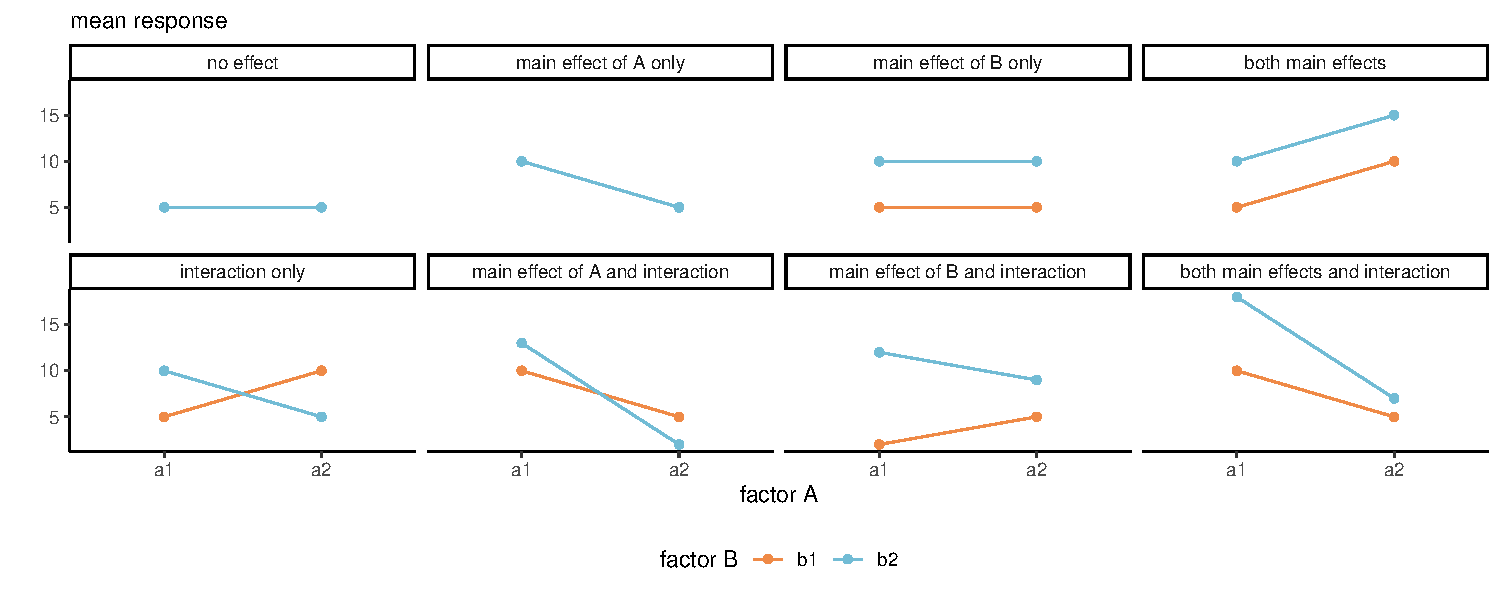
\includegraphics[width=1\textwidth,height=\textheight]{05-interactions_multiway_files/figure-pdf/fig-2by2-1.pdf}

}

\caption{\label{fig-2by2}Interaction plots (line graphs) for example
patterns for means for each of the possible kinds of general outcomes in
a 2 by 2 design. Illustration adapted from Figure 10.2 of Crump,
Navarro, and Suzuki (2019) by Matthew Crump (CC BY-SA 4.0 license).}

\end{figure}

To better understand, we consider the average response and suppose we
have access to the true population average for each sub-treatment. We
can then represent the population using a line graph with the two
factors, one being mapped to color and another to the \(x\)-axis.
Figure~\ref{fig-2by2} shows what happens under all possible scenarios
with a 2 by 2 design. When there is no overall effect, the mean is
constant. If there isn't a main effect of \(A\), the average of the two
mean response for \(a_1\) and \(a_2\) are the same, etc. Interactions
are depicted by \textbf{non-parallel lines}.

It's clear from Figure~\ref{fig-2by2} that looking only at the average
of \(A\) alone (the main effect) isn't instructive when we are in the
presence of an interaction: rather, we should be comparing the values of
\(A\) for \(b_1\) separately than those for \(b_2\), and vice-versa,
using simple effects, otherwise our conclusions may be misleading.

\begin{example}[Interaction plots for Maglio and Polman
(2014)]\protect\hypertarget{exm-MP14-interaction}{}\label{exm-MP14-interaction}

The hypothesis of interest is the interaction; for the time being, we
can simply plot the average per group. Since the summary statistics can
hide important information such as the uncertainty, we add 95\%
confidence intervals for the subgroup averages and superimpose jittered
observations to show the spread of the data. Based on
Figure~\ref{fig-interactionplotMP}, there appears to be at least an
interaction between station and direction of travel, in addition to a
main effect for station. Formal hypothesis testing can help check this
intuition.

\begin{figure}[ht!]

{\centering 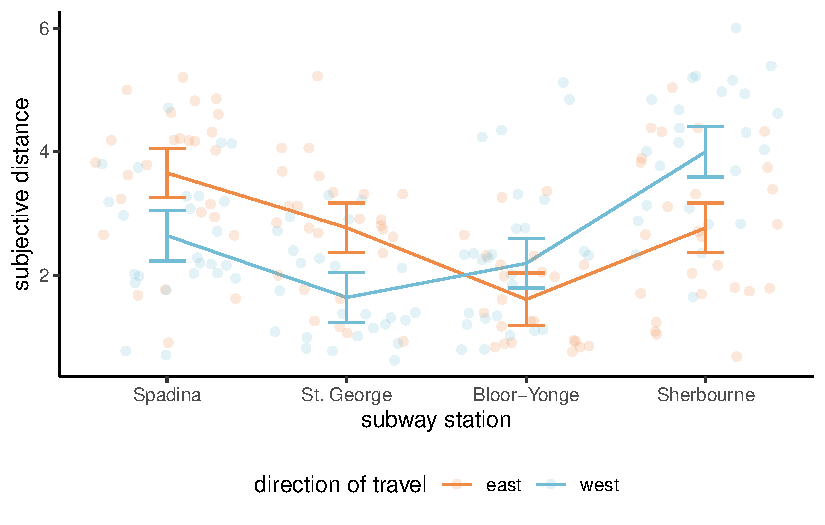
\includegraphics{05-interactions_multiway_files/figure-pdf/fig-interactionplotMP-1.pdf}

}

\caption{\label{fig-interactionplotMP}Interaction plot for Study 1 of
Maglio and Polman (2014), showing group averages and 95\% confidence
intervals for the means. Observations are overlaid on the graph.}

\end{figure}

\end{example}

\hypertarget{model-parametrization}{%
\section{Model parametrization}\label{model-parametrization}}

The following section is technical and may be omitted.

The model parametrized in terms of subgroup or cell average is okay in
Equation~\ref{eq-twowayasoneway}, but it doesn't help us if we want to
check for the presence of main effects and interaction, even if it would
be possible to specify the contrasts required to test these hypotheses.
We can however express the model in terms of main effects and
interactions.

We consider the alternative formulation \begin{align*}
Y_{ijk} = \mu + \alpha_i + \beta_j + (\alpha\beta)_{ij} + \varepsilon_{ijk},
\end{align*} where

\begin{itemize}
\tightlist
\item
  \(\mu\) is the average of all subgroup averages, termed overall mean.
\item
  \(\alpha_i = \mu_{i.} - \mu\) is the mean of level \(A_i\) minus the
  overall mean.
\item
  \(\beta_j = \mu_{.j} - \mu\) is the mean of level \(B_j\) minus
  overall mean.
\item
  \((\alpha\beta)_{ij} = \mu_{ij} - \mu_{i.} - \mu_{.j} + \mu\) is the
  interaction term for \(A_i\) and \(B_j\) which encodes the effect of
  both variable not already captured by the main effects.
\end{itemize}

A rapid calculation shows that there are more coefficients than the
number of cells and subgroups (\(n_an_b\) cells overall) in our table.
The model is \textbf{overparametrized}: to get away with this, we impose
constraints to remove redundancies. The idea is that if we know
\(n_a-1\) of the mean for factor \(A\) and the global average is a
combination of these, we can deduce the value for the last row mean. The
model formulation in terms of difference from the global average or main
effect ensures that we can test for main effects for factor \(A\) by
setting \(\mathscr{H}_0: \alpha_1 = \cdots = \alpha_{n_a-1}=0\). The
\(1 + n_a + n_b\) \textbf{sum to zero} constraints,
\[\sum_{i=1}^{n_a} \alpha_i=0, \quad \sum_{j=1}^{n_b} \beta_j=0, \quad  \sum_{j=1}^{n_b} (\alpha\beta)_{ij}=0, \quad \sum_{i=1}^{n_a} (\alpha\beta)_{ij}=0,\]
restore identifiability.

The redundancy in information, due to the fact main effects are
expressible as row and column averages, and the overall mean as the
average of all observations, will arise again when we consider degrees
of freedom for tests.

\textbf{To be continued}\ldots{}

\begin{example}[Testing for Psychological ownership of borrowed
money]\protect\hypertarget{exm-borrowed-money-test}{}\label{exm-borrowed-money-test}

Sharma, Tully, and Cryder (2021) first proceeded with the test for the
interaction. Since there are one global average and two main effect
(additional difference in average for both factors \texttt{debttype} and
\texttt{purchase}), the interaction involves one degree of freedom since
we go from a model with three parameters describing the mean to one that
has a different average for each of the four subgroups.

The reason why this is first test to carry out is that if the effect of
one factor depends on the level of the other, as shown in
Figure~\ref{fig-2by2}, then we need to compare the label of debt type
separately for each type of purchase and vice-versa using simple
effects. If the interaction on the contrary isn't significant, then we
could pool observations instead and average across either of the two
factors, resulting in the marginal comparisons with the main effects.

Fitting the model including the interaction between factors ensures that
we keep the additivity assumption and that our conclusions aren't
misleading: the price to pay is additional mean parameters to be
estimated, which isn't an issue if you collect enough data, but can be
critical when data collection is extremely costly and only a few runs
are allowed.

In \textbf{R}, we include both factors in a formula as
\texttt{response\ \textasciitilde{}\ factorA\ *\ factorB}, the
\texttt{*} symbol indicating that both are allowed to interact; in the
main effect model, we would use instead \texttt{+} to reflect that the
effects of both factors add up.

\begin{Shaded}
\begin{Highlighting}[]
\CommentTok{\# Analysing Supplementary Study 5}
\CommentTok{\# of Sharma, Tully, and Cryder (2021)}
\FunctionTok{data}\NormalTok{(STC21\_SS5, }\AttributeTok{package =} \StringTok{"hecedsm"}\NormalTok{)}
\NormalTok{mod }\OtherTok{\textless{}{-}} \FunctionTok{aov}\NormalTok{(likelihood }\SpecialCharTok{\textasciitilde{}}\NormalTok{ purchase}\SpecialCharTok{*}\NormalTok{debttype, }
           \AttributeTok{data =}\NormalTok{ STC21\_SS5)}
\FunctionTok{model.tables}\NormalTok{(mod, }\AttributeTok{type =} \StringTok{"means"}\NormalTok{)}
\end{Highlighting}
\end{Shaded}

\begin{verbatim}
Tables of means
Grand mean
         
4.879747 

 purchase 
    discretionary    need
            4.182   5.579
rep       751.000 750.000

 debttype 
     credit    loan
      5.127   4.631
rep 753.000 748.000

 purchase:debttype 
               debttype
purchase        credit loan 
  discretionary   4.5    3.8
  rep           392.0  359.0
  need            5.7    5.4
  rep           361.0  389.0
\end{verbatim}

\begin{Shaded}
\begin{Highlighting}[]
\CommentTok{\# Analysis of variance reveals }
\CommentTok{\# non{-}significant interaction}
\CommentTok{\# of purchase and type}
\NormalTok{car}\SpecialCharTok{::}\FunctionTok{Anova}\NormalTok{(mod, }\AttributeTok{type =} \DecValTok{3}\NormalTok{)}
\end{Highlighting}
\end{Shaded}

\begin{verbatim}
Anova Table (Type III tests)

Response: likelihood
                   Sum Sq   Df   F value    Pr(>F)    
(Intercept)        7974.0    1 1040.9610 < 2.2e-16 ***
purchase            282.8    1   36.9137 1.563e-09 ***
debttype             88.5    1   11.5483 0.0006959 ***
purchase:debttype    13.7    1    1.7852 0.1817132    
Residuals         11467.4 1497                        
---
Signif. codes:  0 '***' 0.001 '**' 0.01 '*' 0.05 '.' 0.1 ' ' 1
\end{verbatim}

\begin{Shaded}
\begin{Highlighting}[]
\CommentTok{\# Main effects}
\NormalTok{emmeans}\SpecialCharTok{::}\FunctionTok{emmeans}\NormalTok{(mod, }
                 \AttributeTok{specs =} \StringTok{"debttype"}\NormalTok{,}
                 \AttributeTok{contr =} \StringTok{"pairwise"}\NormalTok{)}
\end{Highlighting}
\end{Shaded}

\begin{verbatim}
NOTE: Results may be misleading due to involvement in interactions
\end{verbatim}

\begin{verbatim}
$emmeans
 debttype emmean    SE   df lower.CL upper.CL
 credit     5.12 0.101 1497     4.93     5.32
 loan       4.63 0.101 1497     4.43     4.83

Results are averaged over the levels of: purchase 
Confidence level used: 0.95 

$contrasts
 contrast      estimate    SE   df t.ratio p.value
 credit - loan    0.496 0.143 1497   3.469  0.0005

Results are averaged over the levels of: purchase 
\end{verbatim}

\begin{Shaded}
\begin{Highlighting}[]
\CommentTok{\# Pairwise comparisons within levels of purchase}
\CommentTok{\# Simple effect}
\NormalTok{emmeans}\SpecialCharTok{::}\FunctionTok{emmeans}\NormalTok{(mod, }
                 \AttributeTok{specs =} \FunctionTok{c}\NormalTok{(}\StringTok{"purchase"}\NormalTok{, }\StringTok{"debttype"}\NormalTok{),}
                 \AttributeTok{by =} \StringTok{"purchase"}\NormalTok{,}
                 \AttributeTok{contr =} \StringTok{"pairwise"}\NormalTok{)}
\end{Highlighting}
\end{Shaded}

\begin{verbatim}
$emmeans
purchase = discretionary:
 debttype emmean    SE   df lower.CL upper.CL
 credit     4.51 0.140 1497     4.24     4.78
 loan       3.82 0.146 1497     3.54     4.11

purchase = need:
 debttype emmean    SE   df lower.CL upper.CL
 credit     5.74 0.146 1497     5.45     6.02
 loan       5.43 0.140 1497     5.16     5.71

Confidence level used: 0.95 

$contrasts
purchase = discretionary:
 contrast      estimate    SE   df t.ratio p.value
 credit - loan    0.687 0.202 1497   3.398  0.0007

purchase = need:
 contrast      estimate    SE   df t.ratio p.value
 credit - loan    0.305 0.202 1497   1.508  0.1318
\end{verbatim}

In the analysis of variance table, we focus exclusively on the last line
with the sum of squares for \texttt{purchase:debttype}. The \(F\)
statistic is 1.79; using the \(\mathsf{F}\) (1, 1497) distribution as
benchmark, we obtain a \(p\)-value of 0.18 so there is no evidence the
effect of purchase depends on debt type.

We can thus pool data and look at the effect of debt type (\texttt{loan}
or \texttt{credit}) overall by combining the results for all purchase
types, one of the planned comparison reported in the Supplementary
material. To do this in \textbf{R} with the \texttt{emmeans} package, we
use the \texttt{emmeans} function and we quote the factor of interest
(i.e., the one we want to keep) in \texttt{specs}. By default, this will
compute the estimate marginal means: the \texttt{contr\ =\ "pairwise"}
indicates that we want the difference between the two, which gives us
the contrasts.

To get the simple effects, we give both variables in \texttt{specs} as
factors for which to compute subgroup means, then set additionally the
\texttt{by} command to specify which variable we want separate results
for. We get the difference in average between \texttt{credit} and
\texttt{loan} labels for each purchase type along with the \(t\)
statistics for the marginal contrast and the \(p\)-value. The simple
effects suggest that the label has an impact on perception only for
discretionary expenses rather than needed ones, which runs
counter-intuitively with the lack of interaction.

\end{example}

Maglio and Polman (2014) considered the relative perception of distance
from Bay station in Toronto. We modify the data so that we consider
station distance in direction of travel (rather than station names). The
categorical variable \texttt{stdist} has labels \((-2, -1, +1, +2\)) for
stations Spadina, St.~Georges, Bloor-Yonge, Sherbourne in direction
East, and opposite signs in the other direction: see
Figure~\ref{fig-Torontosubway} for the map. We are interested in knowing
whether two stations behind (\texttt{stdist}\(=-2\)) is perceived the
same as two stations ahead (\texttt{stdist}\(=+2\)).

\begin{figure}[ht!]

{\centering 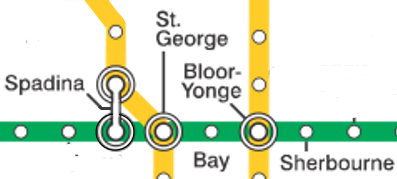
\includegraphics[width=3.29in,height=\textheight]{figures/Toronto_subway.png}

}

\caption{\label{fig-Torontosubway}Simplified depiction of the Toronto
metro stations used in the experiment, based on work by Craftwerker on
Wikipedia, distributed under CC-BY-SA 4.0.}

\end{figure}

\begin{Shaded}
\begin{Highlighting}[]
\CommentTok{\# Set up parametrization to sum{-}to{-}zero for categorical factors}
\FunctionTok{options}\NormalTok{(}\AttributeTok{contrasts =} \FunctionTok{c}\NormalTok{(}\StringTok{"contr.sum"}\NormalTok{, }\StringTok{"contr.poly"}\NormalTok{))}
\FunctionTok{library}\NormalTok{(emmeans)}
\NormalTok{mod }\OtherTok{\textless{}{-}} \FunctionTok{lm}\NormalTok{(distance }\SpecialCharTok{\textasciitilde{}}\NormalTok{ stdist }\SpecialCharTok{*}\NormalTok{ direction, }\AttributeTok{data =}\NormalTok{ MP14\_S1) }
\NormalTok{car}\SpecialCharTok{::}\FunctionTok{Anova}\NormalTok{(mod, }\AttributeTok{type =} \DecValTok{2}\NormalTok{)}
\end{Highlighting}
\end{Shaded}

\hypertarget{tbl-ANOVA2-MP14}{}
\begin{table}
\caption{\label{tbl-ANOVA2-MP14}Analysis of variance (type II effects) for the Maglio and Polman (2014)
reformated data. }\tabularnewline

\centering
\begin{tabular}{lrrrl}
\toprule
term & sum of squares & df & stat & p-value\\
\midrule
stdist & 121.87 & 3 & 37.86 & <0.001\\
direction & 0.38 & 1 & 0.35 & 0.55\\
stdist:direction & 5.70 & 3 & 1.77 & 0.15\\
Residuals & 208.15 & 194 &  & NA\\
\bottomrule
\end{tabular}
\end{table}

We look at the analysis of variance in Table~\ref{tbl-ANOVA2-MP14} to
see what the perception of distance is. The \(F\)-tests suggest that
there is no interaction, and no effect of direction of travel although
there is an uninteresting main effect of station distance (of course,
two station apart is considered further from Bay than one station
apart).

Since there is no interaction, we can collapse the data to a one-way
ANOVA with a single factor (station distance) and consider contrasts.
Say we are interested in testing the perception of distance, by looking
at average distance of pairs at equal distance \(\mu_{-1} = \mu_{+1}\)
and \(\mu_{-2} = \mu_{+2}\).

\begin{figure}[ht!]

{\centering 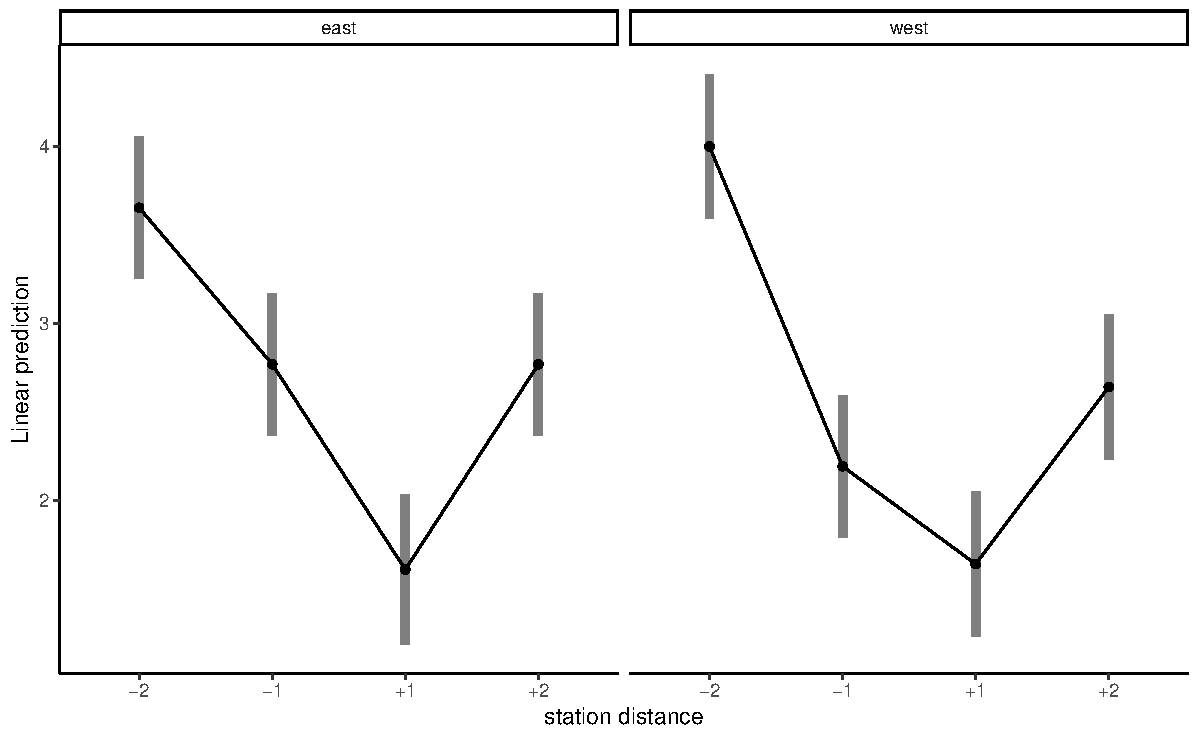
\includegraphics{05-interactions_multiway_files/figure-pdf/fig-interactionMP-1.pdf}

}

\caption{\label{fig-interactionMP}Interaction plot for the reformated
data from Maglio and Polman (2014) with 95\% confidence intervals.}

\end{figure}

If we have categories are in the order \((-2, -1, +1, +2)\), the
contrast weights are \((-1, 0, 0, 1)\) and \((0, -1, 1, 0)\) or a
multiple thereof; the two contrasts are orthogonal.
Table~\ref{tbl-contrast-MP14} shows the result of the hypothesis tests:
both are significant, even applying a Bonferroni correction. This
supports the hypothesis of Maglio and Polman (2014).

\hypertarget{tbl-contrast-MP14}{}
\begin{table}
\caption{\label{tbl-contrast-MP14}Contrasts for comparing the perceived distance for stations at the same
distance on the network, but in opposition directions to that of travel. }\tabularnewline

\centering
\begin{tabular}{lrrrl}
\toprule
contrast & estimate & std. error & stat & p-value\\
\midrule
two dist & -1.12 & 0.21 & -5.47 & <0.001\\
one dist & -0.86 & 0.21 & -4.13 & <0.001\\
\bottomrule
\end{tabular}
\end{table}

It is important to understand that any multiway ANOVA with two or more
factor can be collapsed into a single one-way ANOVA: this is notably
useful when there is a control group which is not related to the factor
levels, as no manipulation takes place. The use of contrasts becomes
critical since we can write any test for main effects, interactions
using the latter through weighting.

\begin{example}[Perceptions of cultural appropriation by
ideology]\protect\hypertarget{exm-LKUK24}{}\label{exm-LKUK24}

We consider a three-way ANOVA from Lin et al. (2024). Their Study 4
focused on cultural appropriation for soul food recipe cookbook from
Chef Dax, who was either black (or not), manipulating the description of
the way he obtained the recipes (by peeking without permission in
kitchens, by asking permission or no mention for control). Authors
postulated that the perception of appropriation would vary by political
ideology (liberal or conservative). The study results in a 3 by 2 by 2
three-way between-subject ANOVA.

For the \(K\)-way ANOVA, we always start with estimating the full model
with all \(K\)-way interaction (provided there are enough data to
estimate the latter, which implies there are repetitions). If the latter
is significant, we can fix one or more factor levels and compare the
others.

\hypertarget{tbl-anova-LKUK24}{}
\begin{table}
\caption{\label{tbl-anova-LKUK24}Analysis of variance table (type II decomposition) for the data from
Study 4 of Lin et al. (2024). }\tabularnewline

\centering
\begin{tabular}{lrrrl}
\toprule
term & sum of squares & df & stat & p-value\\
\midrule
politideo & 48.49 & 1 & 21.35 & <0.001\\
chefdax & 473.72 & 1 & 208.61 & <0.001\\
brandaction & 34.24 & 2 & 7.54 & <0.001\\
politideo:chefdax & 65.00 & 1 & 28.63 & <0.001\\
politideo:brandaction & 1.56 & 2 & 0.34 & 0.71\\
chefdax:brandaction & 0.62 & 2 & 0.14 & 0.87\\
politideo:chefdax:brandaction & 0.66 & 2 & 0.15 & 0.86\\
Residuals & 1587.33 & 699 &  & NA\\
\bottomrule
\end{tabular}
\end{table}

If we consider Table~\ref{tbl-anova-LKUK24}, we find that there is no
three-way interaction and, omitting the latter and focusing on
lower-level, a single two-way interaction between political ideology and
the race of Chef Dax. We cannot interpret the \(p\)-value for the main
effect of \texttt{brandaction}, but we could look at the marginal means.

Based on the data, we will collapse data to a one-way ANOVA comparing
the three levels of \texttt{brandaction} and a 2 by 2 two-way ANOVA for
the other two factors. The results are obtained by averaging over the
missing factor.

We are interested in comparing the perception between the race of Chef
Dax (black or not, as Southern Soul food cooking is more likely to be
associated with cultural appropriation is Chef Dax is not black. We
proceed with \texttt{emmeans} by computing the marginal means separately
for each of the four subcategories, but compare the race of Chef Dax
separately for liberals and conservatives due to the presence of the
interaction.

\begin{Shaded}
\begin{Highlighting}[]
\FunctionTok{data}\NormalTok{(LKUK24\_S4, }\AttributeTok{package =} \StringTok{"hecedsm"}\NormalTok{)}
\NormalTok{mod }\OtherTok{\textless{}{-}} \FunctionTok{lm}\NormalTok{(appropriation }\SpecialCharTok{\textasciitilde{}}\NormalTok{ politideo }\SpecialCharTok{*}\NormalTok{ chefdax }\SpecialCharTok{*}\NormalTok{ brandaction,}
   \AttributeTok{data =}\NormalTok{ LKUK24\_S4)}
\CommentTok{\# Marginal means for political ideology/Chef Dax}
\NormalTok{emm\_racebypolit }\OtherTok{\textless{}{-}} \FunctionTok{emmeans}\NormalTok{(mod, }\AttributeTok{specs =} \StringTok{"chefdax"}\NormalTok{, }\AttributeTok{by =} \StringTok{"politideo"}\NormalTok{)}
\NormalTok{emm\_racebypolit }\SpecialCharTok{|\textgreater{}} \FunctionTok{pairs}\NormalTok{() }\CommentTok{\#shortcut for contrast("pairwise")}
\end{Highlighting}
\end{Shaded}

\begin{verbatim}
politideo = conservative:
 contrast          estimate    SE  df t.ratio p.value
 not black - black     0.71 0.206 699   3.438  0.0006

politideo = liberal:
 contrast          estimate    SE  df t.ratio p.value
 not black - black     2.03 0.135 699  14.998  <.0001

Results are averaged over the levels of: brandaction 
\end{verbatim}

We see that the liberals are much more likely to view Chef Dax cookbook
as an instance of cultural appropriation if he is not black; there is
limited evidence of any difference between conservatives and liberal
when Chef Dax is black. Both differences are statistically
significative, but the differences (and thus evidence of an effect) is
much stronger for left-leaning respondents.

We can look next at the brand action: we expect participants will view
peeking less favorably than if Chef Dax asked for permission to publish
the recipes. It's tricky to know the effect of the control, as we are
not bringing the point to the attention of participants in this
instance.

\begin{Shaded}
\begin{Highlighting}[]
\CommentTok{\# Marginal mean for brandaction}
\NormalTok{emm\_brand }\OtherTok{\textless{}{-}} \FunctionTok{emmeans}\NormalTok{(mod, }\AttributeTok{specs =} \FunctionTok{c}\NormalTok{(}\StringTok{"brandaction"}\NormalTok{)) }
\NormalTok{emm\_brand}
\end{Highlighting}
\end{Shaded}

\begin{verbatim}
 brandaction emmean    SE  df lower.CL upper.CL
 peeking       2.56 0.108 699     2.35     2.77
 permission    2.29 0.105 699     2.09     2.50
 control       2.07 0.108 699     1.86     2.28

Results are averaged over the levels of: politideo, chefdax 
Confidence level used: 0.95 
\end{verbatim}

\begin{Shaded}
\begin{Highlighting}[]
\CommentTok{\# Joint test for the main effect of brandaction}
\NormalTok{emm\_brand }\SpecialCharTok{|\textgreater{}} \FunctionTok{pairs}\NormalTok{() }\SpecialCharTok{|\textgreater{}} \FunctionTok{joint\_tests}\NormalTok{()}
\end{Highlighting}
\end{Shaded}

\begin{verbatim}
 model term df1 df2 F.ratio p.value
 contrast     2 699   5.091  0.0064
\end{verbatim}

A joint \(F\)-test, obtained by collapsing everything to a one-way
ANOVA, shows that there are indeed differences. However, note that the
averages of the three actions are much smaller than for race.

\end{example}

\begin{tcolorbox}[enhanced jigsaw, colback=white, coltitle=black, rightrule=.15mm, left=2mm, bottomrule=.15mm, toprule=.15mm, titlerule=0mm, colframe=quarto-callout-important-color-frame, leftrule=.75mm, title=\textcolor{quarto-callout-important-color}{\faExclamation}\hspace{0.5em}{\textbf{Summary}}, breakable, arc=.35mm, colbacktitle=quarto-callout-important-color!10!white, opacitybacktitle=0.6, opacityback=0, toptitle=1mm, bottomtitle=1mm]

\begin{itemize}
\tightlist
\item
  Complete factorial designs consist of experiments in which we
  manipulate multiple experimental factors at once and collect
  observations for each subgroup.
\item
  Factorial designs are more efficient than running repeatedly one-way
  analysis of variance with the same sample size per group.
\item
  Interactions occur when the effect of a variable depends on the levels
  of the others.
\item
  Interaction plots (group average per group) can help capture this
  difference, but beware of overinterpretation in small samples.
\item
  If there is an interaction, we consider differences and contrasts for
  each level of the other factor (\textbf{simple effects}).
\item
  If there is no interaction, we can pool observations and look at
  \textbf{main effects}.
\item
  A multiway analysis of variance can be treated as a one-way analysis
  of variance by collapsing categories; however, only specific contrasts
  will be of interest.
\item
  The number of observations increases quickly with the dimension as we
  increase the number of factors considered.
\end{itemize}

\end{tcolorbox}

\bookmarksetup{startatroot}

\hypertarget{designs-to-reduce-the-error}{%
\chapter{Designs to reduce the
error}\label{designs-to-reduce-the-error}}

The previous chapter dealt with factorial experiments in which all
experimental factors are of interest. It is possible to use measurements
concomitant to the data collection (for example, value to a test before
we complete the group assignment for the manipulation) to get a measure
of the relative strength of students. The more correlated these measures
are with the response, the more we can explain the data. We then proceed
with the random assignment of our experimental units to different
conditions.

Including blocking factor or covariates should in principle increase
power and our ability to detect real differences due to experimental
manipulations, provided the variables used as control are correlated
with the response. Generally, they are not needed for valid inference,
which is guaranteed by randomization, and shouldn't be used to assign
treatment.

\hypertarget{blocking-factors}{%
\section{Blocking factors}\label{blocking-factors}}

In many instances, some of the characteristics of observational units
are not of interest: for example, EEG measurements of participants in a
lab may differ due to time of the day, to the lab technician, etc. These
are instances of \textbf{blocking factors}: variables that impact the
measurement variability, but that are not of direct interest. By
filtering their effect out and looking at the residual variability that
is unexplained by the blocking factors. Block designs reduce the error
term, at the cost of including and estimating additional parameters
(group averages). Experimental units are typically assigned to blocking
factor using stratified sampling to ensure comparisons can be made.

We will analyse block designs in the same as we did for multi-way
analysis of variance model, with one notable exception. Typically, we
will assume that there is \textbf{no interaction} between experimental
factor and blocking factors.\footnote{We can always check for this
  assumption.} Thus, we will be interested mostly in main effects of the
experimental factors.

\begin{example}[The surprise of reaching out: paired data as blocking
factors]\protect\hypertarget{exm-reachingout}{}\label{exm-reachingout}

We consider paired data from Study 3 of Liu et al. (2023), who looked at
the appreciation of people reaching out to them in a unsolicited manner.
The data includes the appreciation score of both responder and
initiator, along with sociodemographic variables (age and gender).

While a paired \(t\)-test is the natural (and arguably simplest way) to
compare the difference in appreciation scores, we reformat the data to
long format (one response per line), with a categorical variable
\texttt{role} indicating the role of the participant and \texttt{dyad},
a dummy number indicating which participants belong to which pair. We
then fit an analysis of variance model to the scores with both
\texttt{dyad} and \texttt{role}. The \(F\)-tests for the main effects
indicate that the dyads (66 additional parameters, since there are 67
pairs) filter out significant part of the variability. If we consider
estimated marginal means and look at the \(p\)-value and the pairwise
difference between initiator and respondent, we find exactly the same
statistic, degrees of freedom and \(p\)-value for the pairwise
difference as the paired \(t\)-test.

\begin{Shaded}
\begin{Highlighting}[]
\FunctionTok{data}\NormalTok{(LRMM23\_S3, }\AttributeTok{package =} \StringTok{"hecedsm"}\NormalTok{)}
\CommentTok{\# Paired t{-}tests}
\FunctionTok{with}\NormalTok{(LRMM23\_S3, }\FunctionTok{t.test}\NormalTok{(apprec\_init, apprec\_resp, }\AttributeTok{paired =} \ConstantTok{TRUE}\NormalTok{))}
\end{Highlighting}
\end{Shaded}

\begin{verbatim}

    Paired t-test

data:  apprec_init and apprec_resp
t = -4.6042, df = 66, p-value = 1.94e-05
alternative hypothesis: true mean difference is not equal to 0
95 percent confidence interval:
 -0.6633265 -0.2620466
sample estimates:
mean difference 
     -0.4626866 
\end{verbatim}

\begin{Shaded}
\begin{Highlighting}[]
\CommentTok{\# Cast data to long format {-} one response/participant per line}
\NormalTok{LRMM23\_S3l }\OtherTok{\textless{}{-}}\NormalTok{ LRMM23\_S3 }\SpecialCharTok{|\textgreater{}}
\NormalTok{  dplyr}\SpecialCharTok{::}\FunctionTok{mutate}\NormalTok{(}\AttributeTok{dyad =} \FunctionTok{factor}\NormalTok{(dplyr}\SpecialCharTok{::}\FunctionTok{row\_number}\NormalTok{())) }\SpecialCharTok{|\textgreater{}} 
\NormalTok{  tidyr}\SpecialCharTok{::}\FunctionTok{pivot\_longer}\NormalTok{(}
    \AttributeTok{cols =} \SpecialCharTok{!}\NormalTok{dyad, }
    \AttributeTok{names\_to =} \FunctionTok{c}\NormalTok{(}\StringTok{".value"}\NormalTok{, }\StringTok{"role"}\NormalTok{),}
    \AttributeTok{names\_sep =} \StringTok{"}\SpecialCharTok{\textbackslash{}\textbackslash{}}\StringTok{\_"}\NormalTok{)}
\CommentTok{\# Format of the data}
\FunctionTok{head}\NormalTok{(LRMM23\_S3l)}
\end{Highlighting}
\end{Shaded}

\begin{verbatim}
# A tibble: 6 x 5
  dyad  role  apprec   age gender
  <fct> <chr>  <int> <dbl> <fct> 
1 1     resp       4    20 male  
2 1     init       4    20 male  
3 2     resp       5    20 female
4 2     init       5    24 female
5 3     resp       5    21 female
6 3     init       4    21 female
\end{verbatim}

\begin{Shaded}
\begin{Highlighting}[]
\CommentTok{\# Treat dyad as a factor and fit two{-}way ANOVA model}
\NormalTok{mod }\OtherTok{\textless{}{-}} \FunctionTok{lm}\NormalTok{(apprec }\SpecialCharTok{\textasciitilde{}}\NormalTok{ role }\SpecialCharTok{+}\NormalTok{ dyad, }\AttributeTok{data =}\NormalTok{ LRMM23\_S3l)}
\CommentTok{\# Global tests of main effects (balanced data)}
\FunctionTok{anova}\NormalTok{(mod) }\CommentTok{\# There seems to be significant variability filtered out by \textquotesingle{}id\textquotesingle{}}
\end{Highlighting}
\end{Shaded}

\begin{verbatim}
Analysis of Variance Table

Response: apprec
          Df Sum Sq Mean Sq F value    Pr(>F)    
role       1  7.172  7.1716 21.1985  1.94e-05 ***
dyad      66 51.970  0.7874  2.3275 0.0003759 ***
Residuals 66 22.328  0.3383                      
---
Signif. codes:  0 '***' 0.001 '**' 0.01 '*' 0.05 '.' 0.1 ' ' 1
\end{verbatim}

\begin{Shaded}
\begin{Highlighting}[]
\CommentTok{\# Compute pairwise difference for main effect of \textquotesingle{}role\textquotesingle{}}
\NormalTok{emmeans}\SpecialCharTok{::}\FunctionTok{emmeans}\NormalTok{(mod, }\AttributeTok{spec =} \StringTok{"role"}\NormalTok{) }\SpecialCharTok{|\textgreater{}}
\NormalTok{  emmeans}\SpecialCharTok{::}\FunctionTok{contrast}\NormalTok{(}\StringTok{"pairwise"}\NormalTok{)}
\end{Highlighting}
\end{Shaded}

\begin{verbatim}
 contrast    estimate  SE df t.ratio p.value
 init - resp   -0.463 0.1 66  -4.604  <.0001

Results are averaged over the levels of: dyad 
\end{verbatim}

\end{example}

\hypertarget{ancova}{%
\section{Analysis of covariance}\label{ancova}}

A related design includes a continuous covariate to the analysis of
variance, whose slope governs the relationship with the response. The
strict inclusion isn't necessary to draw valid causal conclusion, but
adding the term helps again reduce the residual variability. Such a
design was historically called \textbf{analysis of covariance}, although
as analysis of variance models, they are nothing but linear regression
models.

In an analysis of covariance, we include a linear component for a
(continuous) covariate, with the purpose again to reduce residual error
and increase power. A prime example is prior/post experiment
measurements, whereby we monitor the change in outcome due to the
manipulation. This post by Solomon Kurz
\href{https://solomonkurz.netlify.app/blog/2023-04-12-boost-your-power-with-baseline-covariates/}{{[}link{]}}
nicely illustrates the added benefits of using covariates when there is
strong correlation between your response and the latter

In such setting, it may seem logical to take the difference in post and
prior score as response: this is showcased in Example~\ref{exm-vanStek}
and Baumann, Seifert-Kessell, and Jones (1992), an analysis of which is
presented on \href{https://edsm.rbind.io/example/06-ancova/}{the course
website}.

When we add a covariate, we need the latter to have a strong linear
correlation for the inclusion to make sense. We can assess graphically
whether the relationship is linear, and whether the slopes for each
experimental condition are the same.\footnote{If not, this implies that
  the covariate interacts with the experimental condition.}

\begin{figure}[ht!]

{\centering 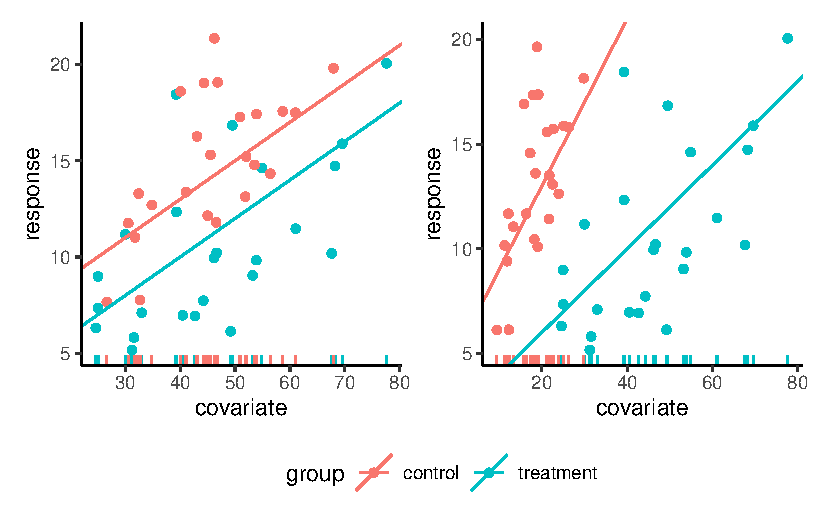
\includegraphics{06-blocking_ancova_files/figure-pdf/fig-ancovadifftrend-1.pdf}

}

\caption{\label{fig-ancovadifftrend}Simulated data from two groups with
an analysis of covariance model.}

\end{figure}

The left panel of Figure~\ref{fig-ancovadifftrend} shows the ideal
situation for an analysis of covariate: the relationship between
response and covariate is linear with strong correlation, with the same
slope and overlapping support. Since the slopes are the same, we can
compare the difference in average (the vertical difference between
slopes at any level of the covariate) because the latter is constant, so
this depiction is useful. By contrast, the right-hand panel of
Figure~\ref{fig-ancovadifftrend} shows an interaction between the
covariate and the experimental groups, different slopes: there, the
effect of the experimental condition increases with the level of the
covariate. One may also note that the lack of overlap in the support,
the set of values taken by the covariate, for the two experimental
conditions, makes comparison hazardous at best in the right-hand panel.

Figure~\ref{fig-ancovaresid} shows that, due to the strong correlation,
the variability of the measurements is smaller on the right-hand panel
(corresponding to the analysis of covariance model) than for the centred
response on the left-hand panel; note that the \(y\)-axes have different
scales.

\begin{figure}[ht!]

{\centering 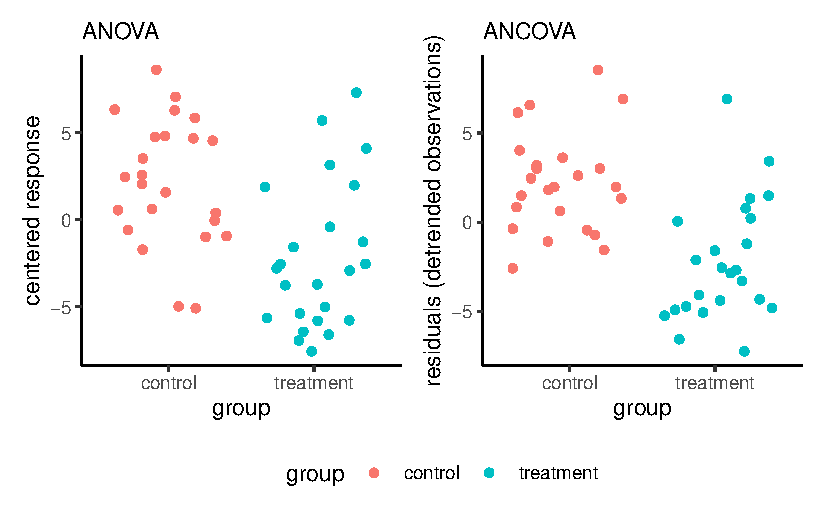
\includegraphics{06-blocking_ancova_files/figure-pdf/fig-ancovaresid-1.pdf}

}

\caption{\label{fig-ancovaresid}Response after subtracting mean (left)
and after detrending (right).}

\end{figure}

We present two examples of analysis of covariance, showing how the
inclusion of covariates helps disentangle differences between
experimental conditions.

\begin{example}[Inconsistency of product description and image in online
retailing]\protect\hypertarget{exm-leechoi}{}\label{exm-leechoi}

Lee and Choi (2019) measured the impact of discrepancies between
descriptions and visual depiction of items in online retail. They
performed an experiment in which participants were presented with
descriptions of a product (a set of six toothbrushes) that was either
consistent or inconsistent with the description. The authors postulated
that a discrepancy could lead to lower appreciation score, measured
using three Likert scales. They also suspected that the familiarity with
the product brand should impact ratings, and controlled for the latter
using another question.

One way to account for familiarity when comparing the mean is to use a
linear regression with familiarity as another explanatory variable. The
expected value of the product evaluation is
\begin{equation}\protect\hypertarget{eq-vS}{}{
\mathsf{E}(\texttt{prodeval}) = \beta_0 + \beta_1 \texttt{familiarity} + \beta_2 \texttt{consistency}, 
}\label{eq-vS}\end{equation} where \(\texttt{familiarity}\) is the score
from 1 to 7 and \(\texttt{consistency}\) is a binary indicator equal to
one if the output is inconsistent and zero otherwise. The coefficient
\(\beta_2\) thus measures the difference between product evaluation
rating for consistent vs inconsistent displays, for the same familiarity
score.

We can look at coefficient (standard error) estimates
\(\widehat{\beta}_2 = -0.64 (0.302)\). No difference between groups
would mean \(\beta_2=0\) and we can build a test statistic by looking at
the standardized regression coefficient
\(t = \widehat{\beta}_2/\mathsf{se}(\widehat{\beta}_2)\). The result
output is \(b = -0.64\), 95\% CI \([-1.24, -0.04]\), \(t(93) = -2.12\),
\(p = .037\). We reject the null hypothesis of equal product evaluation
for both display at level 5\%: there is evidence that there is a small
difference, with people giving on average a score that is 0.64 points
smaller (on a scale of 1 to 9) when presented with conflicting
descriptions and images.

We can compare the analysis of variance table obtained by fitting the
model with and without \(\texttt{familiarity}\).
Table~\ref{tbl-anovatabLC19S1} shows that the effect of consistency is
small and not significant and a two-sample \emph{t}-test shows no
evidence of difference between the average familiarity score in both
experimental conditions (\(p\)-value of \(.532\)). However, we can
explain roughly one fifth of the residual variability by the familiarity
with the brand (see the sum of squares in
Table~\ref{tbl-anovatabLC19S1}): removing the latter leads to a higher
signal-to-noise ratio for the impact of consistency, at the expense of a
loss of one degree of freedom. Thus, it appears that the manipulation
was successful.

\begin{table}

\caption{\label{tbl-anovatabLC19S1}Analysis of variance
tables}\begin{minipage}[t]{\linewidth}
\subcaption{\label{tbl-anovatabLC19S1-1}model without familiarity}

{\centering 

\centering
\begin{tabular}[t]{lrrrl}
\toprule
term & sum. sq. & df & stat & p-value\\
\midrule
consistency & 7.04 & 1 & 2.55 & .113\\
Residuals & 259.18 & 94 &  & \\
\bottomrule
\end{tabular}

}

\end{minipage}%
\newline
\begin{minipage}[t]{\linewidth}
\subcaption{\label{tbl-anovatabLC19S1-2}model with familiarity}

{\centering 

\centering
\begin{tabular}[t]{lrrrl}
\toprule
term & sum. sq. & df & stat & p-value\\
\midrule
familiarity & 55.94 & 1 & 25.60 & < .001\\
consistency & 9.80 & 1 & 4.49 & .037\\
Residuals & 203.24 & 93 &  & \\
\bottomrule
\end{tabular}

}

\end{minipage}%

\end{table}

\begin{figure}[ht!]

{\centering 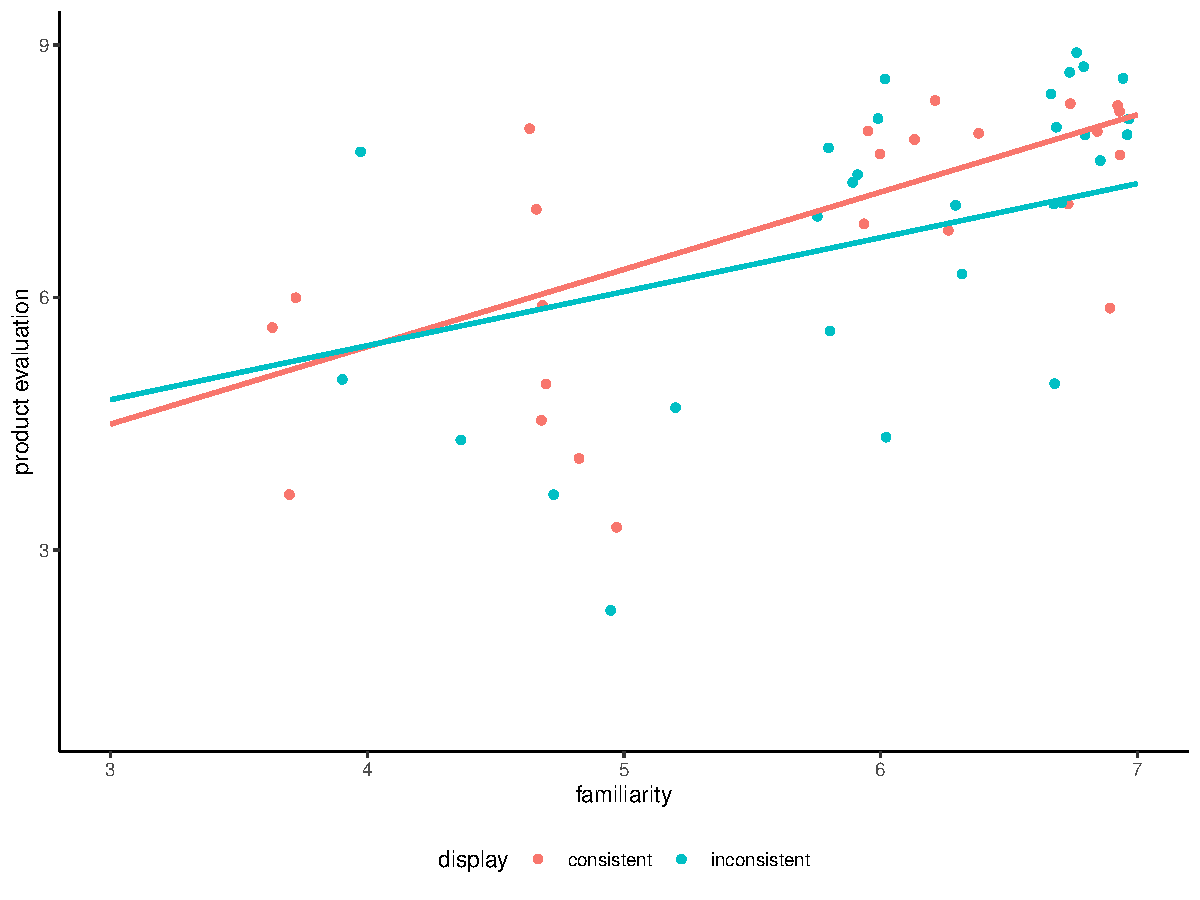
\includegraphics[width=0.7\textwidth,height=\textheight]{06-blocking_ancova_files/figure-pdf/fig-ANCOVA-demo-1.pdf}

}

\caption{\label{fig-ANCOVA-demo}Scatterplot of product evaluation as a
function of the familiarity score, split by experimental manipulation.}

\end{figure}

Figure~\ref{fig-ANCOVA-demo} shows that people more familiar with the
product or brand tend to have a more positive product evaluation, as
postulated by the authors. The graph also shows two straight lines
corresponding to the fit of a linear model with different intercept and
slope for each display group: there is little material difference, one
needs to assess formally whether a single linear relationship as the one
postulated in Equation~\ref{eq-vS} can adequately characterize the
relation in both groups.

To this effect, we fit a linear model with different slopes in each
group, and compare the fit of the latter with the analysis of covariance
model that includes a single slope for both groups: we can then test if
the slopes are the same, or alternatively if the difference between the
slopes is zero. The \emph{t}-statistic indicates no difference in slope
(\(p\)-value of \(.379\)), thus the assumption is reasonable. Levene's
test for homogeneity of variance indicates no discernible difference
between groups. Thus, it appears there is a difference in perception of
product quality due to the manipulation.

\end{example}

\begin{example}[Effect of scientific consensus on false
beliefs]\protect\hypertarget{exm-vanStek}{}\label{exm-vanStek}

We consider Study 3 of Stekelenburg et al. (2021), who studied changes
in perception of people holding false beliefs or denying (to some
extent) the scientific consensus by presenting them with news article
showcasing information about various phenomena. The experimental
manipulation consisted in presenting boosting, a form of training to
help readers identify and establish whether scientifists were truly
expert in the domain of interest, how strong was the consensus,
etc.\footnote{The article is interesting because lack of
  planning/changes led them to adapt the design from experiment 1 to 3
  until they found something. Without preregistration, it is unlikely
  such findings would have been publishable.}

The third and final experiment of the paper focused on genetically
modified organisms: it is a replication of Study 2, but with a control
group (since there were no detectable difference between experimental
conditions \texttt{Boost} and \texttt{BoostPlus}) and a larger sample
size (because Study 2 was underpowered).

The data include 854 observations with \texttt{prior}, the negative of
the prior belief score of the participant, the \texttt{post} experiment
score for the veracity of the claim. Both were measured using a visual
scale ranging from -100 (I am 100\% certain this is false) to 100 (I am
100\% certain this is true), with 0 (I don't know) in the middle. Only
people with negative prior beliefs were recruited to the study. The
three experimental conditions were \texttt{BoostPlus},
\texttt{consensus} and a \texttt{control} group. Note that the scores in
the data have been negated, meaning that negative posterior scores
indicate agreement with the consensus on GMO.

Preliminary checks suggest that, although the slopes for prior beliefs
could plausibly be the same in each group and the data are properly
randomized, there is evidence of unequal variance for the changes in
score. As such, we fit a model with mean \begin{align*}
\mathsf{E}(\texttt{post}) &= \begin{cases}
\beta_0 + \beta_1 \texttt{prior} + \alpha_1 &  \texttt{condition} = \texttt{BoostPlus}\\
\beta_0 + \beta_1 \texttt{prior} + \alpha_2 &\texttt{condition} = \texttt{consensus}\\
\beta_0 + \beta_1 \texttt{prior} + \alpha_3 &\texttt{condition} = \texttt{control}
\end{cases}
\end{align*} with \(\alpha_1 + \alpha_2 + \alpha_3=0\), using the
sum-to-zero parametrization, and with different variance for each
experimental condition, \begin{align*}
\mathsf{Va}(\texttt{post}) = \begin{cases}
\sigma^2_1, &  \texttt{condition} = \texttt{BoostPlus},\\
\sigma^2_2, &  \texttt{condition} = \texttt{consensus},\\
\sigma^2_3, & \texttt{condition} = \texttt{control}.
\end{cases}
\end{align*} Because of the unequal variances, we cannot use multiple
testing procedures reserved for analysis of variance and resort instead
to Holm--Bonferroni to control the familywise error rate. We here look
only at pairwise differences between conditions.\footnote{In Study 2,
  the interest was comparing manipulation vs control and the Boost vs
  BoostPlus conditions, two orthogonal contrasts.}

\begin{table}

\caption{\label{tbl-anovatabSSVB}Analysis of variance
tables}\begin{minipage}[t]{\linewidth}
\subcaption{\label{tbl-anovatabSSVB-1}ANOVA model (without prior belief)}

{\centering 

\centering
\begin{tabular}[t]{lrrl}
\toprule
term & df & stat & p-value\\
\midrule
condition & 2 & 42.5 & < .001\\
\bottomrule
\end{tabular}

}

\end{minipage}%
\newline
\begin{minipage}[t]{\linewidth}
\subcaption{\label{tbl-anovatabSSVB-2}ANCOVA model (with prior belief)}

{\centering 

\centering
\begin{tabular}[t]{lrrl}
\toprule
term & df & stat & p-value\\
\midrule
prior & 1 & 289.2 & < .001\\
condition & 2 & 57.0 & < .001\\
\bottomrule
\end{tabular}

}

\end{minipage}%

\end{table}

Repeating the exercise of comparing the amount of evidence for
comparison with and without inclusion of a covariate shows that the
value of the test statistic is larger (Table~\ref{tbl-anovatabSSVB}),
indicative of stronger evidence with the analysis of covariance model:
the conclusion would be unaffected with such large sample sizes. We of
course care very little for the global \(F\) test of equality of mean,
as the previous study had shown large differences. What is more
interesting here is quantifying the change between conditions.

\begin{table}

\caption{\label{tbl-contraststabSSVB}Pairwise contrasts with
\_p\_-values adjusted using
Holm-\/-Bonferroni}\begin{minipage}[t]{\linewidth}
\subcaption{\label{tbl-contraststabSSVB-1}ANOVA model (without prior belief score).}

{\centering 

\centering
\begin{tabular}[t]{lrrrrl}
\toprule
contrast & estimate & std.error & df & statistic & p.value\\
\midrule
consensus vs control & -11.98 & 4.0 & 557.54 & -3.007 & .003\\
consensus vs BoostPlus & 16.31 & 4.7 & 546.36 & 3.490 & < .001\\
BoostPlus vs control & -28.29 & 4.4 & 505.44 & -6.489 & < .001\\
\bottomrule
\end{tabular}

}

\end{minipage}%
\newline
\begin{minipage}[t]{\linewidth}
\subcaption{\label{tbl-contraststabSSVB-2}ANCOVA model (with prior belief score).}

{\centering 

\centering
\begin{tabular}[t]{lrrrrl}
\toprule
contrast & estimate & std.error & df & statistic & p.value\\
\midrule
consensus vs control & -11.84 & 3.3 & 543.06 & -3.544 & < .001\\
consensus vs BoostPlus & 17.47 & 4.3 & 523.60 & 4.108 & < .001\\
BoostPlus vs control & -29.30 & 3.9 & 458.62 & -7.454 & < .001\\
\bottomrule
\end{tabular}

}

\end{minipage}%

\end{table}

Table~\ref{tbl-contraststabSSVB} shows the pairwise contrasts, which
measure two different things: the analysis of variance model compares
the average in group, whereas the analysis of covariance (the linear
model with \texttt{prior}) uses detrended values and focuses on the
change in perception. Because the data are unbalanced and we estimate
group mean and variance separately, the degrees of freedom change from
one pairwise comparison to the next. Again, using the covariate
\texttt{prior}, which is somewhat strongly correlated with \texttt{post}
as seen in Figure~\ref{fig-vanStekS3}, helps decrease background noise.

\hypertarget{tbl-vanStekS3}{}
\begin{table}
\caption{\label{tbl-vanStekS3}Summary statistics of belief as a function of time of measurement and
experimental condition. }\tabularnewline

\centering
\begin{tabular}{llrr}
\toprule
time & condition & mean & se\\
\midrule
prior & BoostPlus & 57.65 & 1.69\\
prior & consensus & 56.32 & 1.67\\
prior & control & 56.49 & 1.68\\
post & BoostPlus & 2.62 & 3.53\\
post & consensus & 18.93 & 3.06\\
post & control & 30.91 & 2.56\\
\bottomrule
\end{tabular}
\end{table}

\begin{figure}[ht!]

{\centering 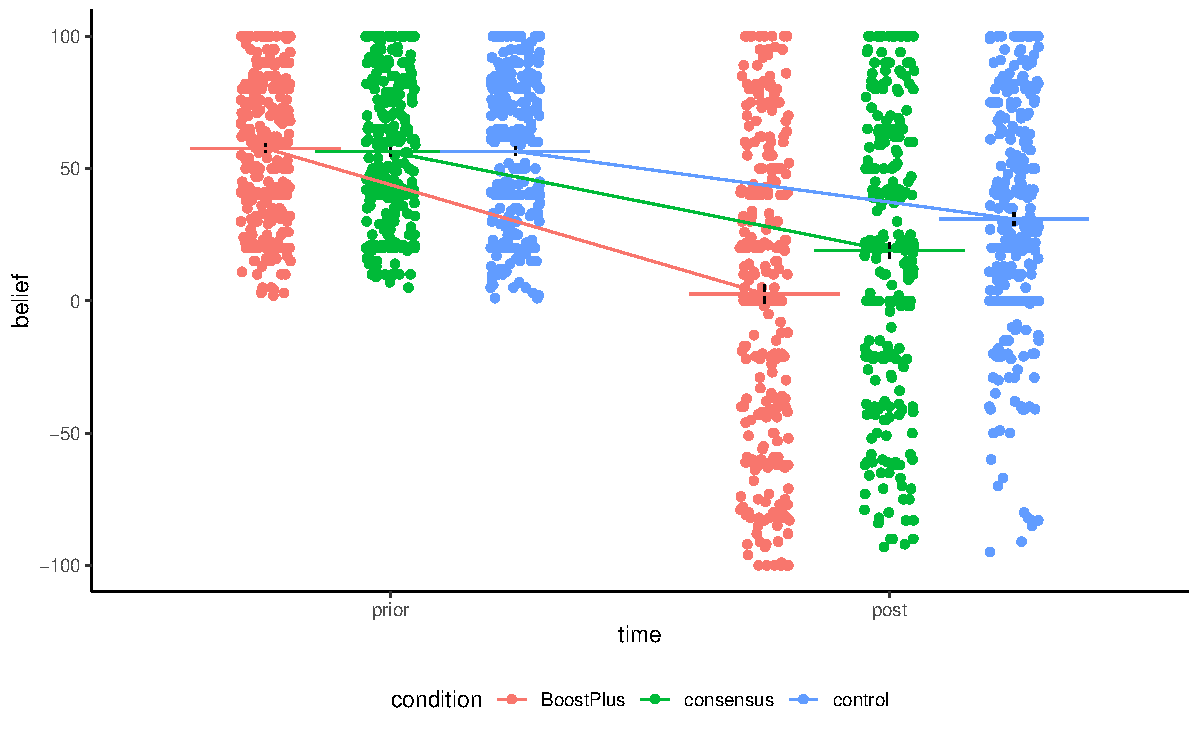
\includegraphics{06-blocking_ancova_files/figure-pdf/fig-vanStekS3-1.pdf}

}

\caption{\label{fig-vanStekS3}Difference between prior and post
experiment beliefs on genetically engineered food.}

\end{figure}

\end{example}

\begin{tcolorbox}[enhanced jigsaw, colback=white, coltitle=black, rightrule=.15mm, left=2mm, bottomrule=.15mm, toprule=.15mm, titlerule=0mm, colframe=quarto-callout-caution-color-frame, leftrule=.75mm, title=\textcolor{quarto-callout-caution-color}{\faFire}\hspace{0.5em}{Pitfall}, breakable, arc=.35mm, colbacktitle=quarto-callout-caution-color!10!white, opacitybacktitle=0.6, opacityback=0, toptitle=1mm, bottomtitle=1mm]

Stekelenburg et al. (2021) split their data to do pairwise comparisons
two at the time (thus taking roughly two-third of the data to perform a
two sample \emph{t}-test with each pair). Although it does not impact
their conclusion, this approach is conceptually incorrect: if the
variance was equal, we would want to use all observations to estimate it
(so their approach would be suboptimal, since we would estimate the
variance three times with smaller samples).

On the contrary, using a model that assumes equal variance when it is
not the case leads to distortion: the variance we estimate will be some
sort of average of the variability \(\sigma_i\) and \(\sigma_j\) in
experimental condition \(i\) and \(j\), again potentially leading to
distortions. With large samples, this may be unconsequential, but
illustrates caveats of subsample analyses.

\end{tcolorbox}

\begin{tcolorbox}[enhanced jigsaw, colback=white, coltitle=black, rightrule=.15mm, left=2mm, bottomrule=.15mm, toprule=.15mm, titlerule=0mm, colframe=quarto-callout-caution-color-frame, leftrule=.75mm, title=\textcolor{quarto-callout-caution-color}{\faFire}\hspace{0.5em}{Pitfall}, breakable, arc=.35mm, colbacktitle=quarto-callout-caution-color!10!white, opacitybacktitle=0.6, opacityback=0, toptitle=1mm, bottomtitle=1mm]

Figure~\ref{fig-vanStekS3f1} shows the relationship between prior and
posterior score. The data show clear difference between individuals:
many start from completely disbelieving of genetically engineered food
and change their mind (sometimes drastically), there are many people who
do not change idea at all and have similar scores, and many who give a
posterior score of zero. This heterogeneity in the data illustrates the
danger of only looking at the summary statistics and comparing averages.
It does not tell the whole picture! One could investigate whether the
strength of religious or political beliefs, or how much participants
trust scientists, could explain some of the observed differences.

\end{tcolorbox}

\begin{figure}[ht!]

{\centering 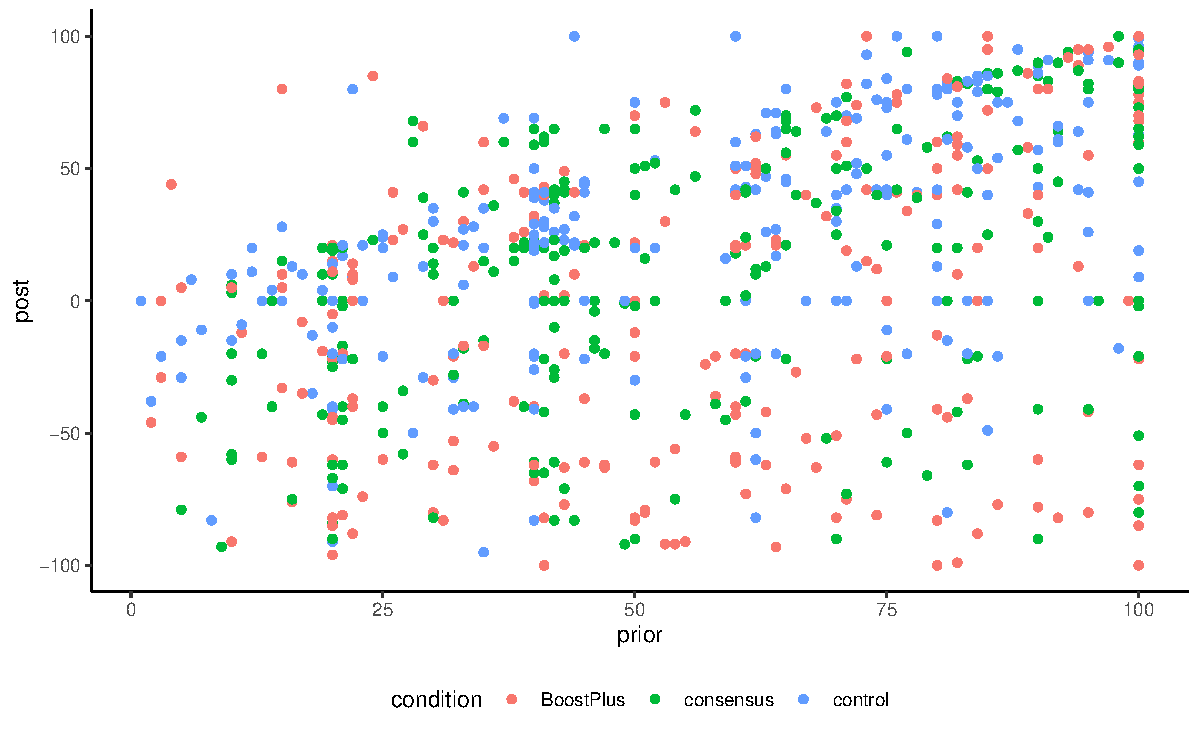
\includegraphics[width=0.8\textwidth,height=\textheight]{06-blocking_ancova_files/figure-pdf/fig-vanStekS3f1-1.pdf}

}

\caption{\label{fig-vanStekS3f1}Scatterplot of negated prior and
posterior belief score.}

\end{figure}

\begin{tcolorbox}[enhanced jigsaw, colback=white, coltitle=black, rightrule=.15mm, left=2mm, bottomrule=.15mm, toprule=.15mm, titlerule=0mm, colframe=quarto-callout-important-color-frame, leftrule=.75mm, title=\textcolor{quarto-callout-important-color}{\faExclamation}\hspace{0.5em}{\textbf{Summary}}, breakable, arc=.35mm, colbacktitle=quarto-callout-important-color!10!white, opacitybacktitle=0.6, opacityback=0, toptitle=1mm, bottomtitle=1mm]

\begin{itemize}
\tightlist
\item
  Inclusion of blocking factor and continuous covariates may help
  filtering out unwanted variability.
\item
  These are typically concomitant variables (measured alongside the
  response variable).
\item
  These designs reduce the residual error, leading to an increase in
  power (more ability to detect differences in average between
  experimental conditions).
\item
  We are only interested in differences due to experimental condition
  (marginal effects).
\item
  In general, there should be no interaction between covariates/blocking
  factors and experimental conditions.
\item
  This hypothesis can be assessed by comparing the models with and
  without interaction, if there are enough units (e.g., equality of
  slope for ANCOVA).
\end{itemize}

\end{tcolorbox}

\begin{tcolorbox}[enhanced jigsaw, colback=white, coltitle=black, rightrule=.15mm, left=2mm, bottomrule=.15mm, toprule=.15mm, titlerule=0mm, colframe=quarto-callout-tip-color-frame, leftrule=.75mm, title=\textcolor{quarto-callout-tip-color}{\faLightbulb}\hspace{0.5em}{Your turn}, breakable, arc=.35mm, colbacktitle=quarto-callout-tip-color!10!white, opacitybacktitle=0.6, opacityback=0, toptitle=1mm, bottomtitle=1mm]

\begin{itemize}
\tightlist
\item
  Box, Hunter, and Hunter (1978) write on page 103 the following motto:
\end{itemize}

\begin{quote}
Block what you can and randomize what you cannot.
\end{quote}

Explain the main benefit of blocking for confounding variables (when
possible) over randomization.

\end{tcolorbox}

\bookmarksetup{startatroot}

\hypertarget{effect-sizes-and-power}{%
\chapter{Effect sizes and power}\label{effect-sizes-and-power}}

In social studies, it is common to write a paper containing multiple
studies on a similar topic. These may use different designs, with
varying sample size. If the studies uses different questionnaires, or
change the Likert scale, the results and the mean difference between
groups are not directly comparable between experiments.

We may also wish replicate a study by using the same material and re-run
an experiment. For the replication to be somewhat successful (or at
least reliable), one needs to determine beforehand how many participants
should be recruited in the study.

We could think for an example of comparing statistics or \(p\)-values,
which are by construction standardized unit less measures, making them
comparable across study. Test statistics show how outlying observed
differences between experimental conditions relative to a null
hypothesis, typically that of no effect (equal mean in each subgroup).
However, statistics are usually a function of both the sample size (the
number of observations in each experimental condition) and the effect
size (how large the standardized differences between groups are), making
them unsuitable for describing differences.

\begin{figure}[ht!]

{\centering 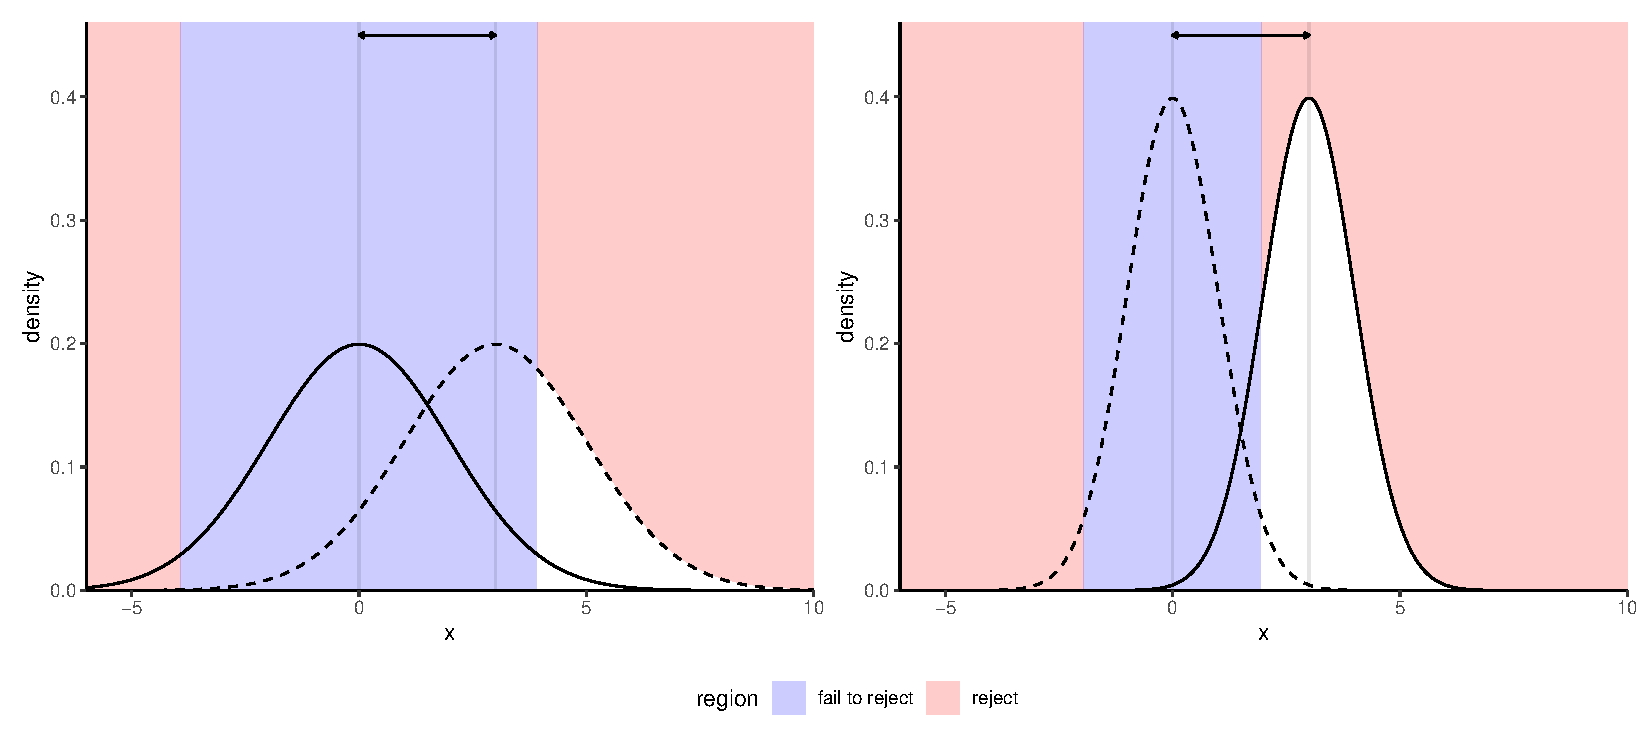
\includegraphics[width=0.9\textwidth,height=\textheight]{07-power_effect_files/figure-pdf/fig-effectsize-1.pdf}

}

\caption{\label{fig-effectsize}True sampling distribution for a
two-sample \(t\)-test under the alternative (rightmost curve) and null
distribution (leftmost curve) with small (left panel) and large (right
panel) sample sizes.}

\end{figure}

Figure~\ref{fig-effectsize} shows an example with the sampling
distributions of the difference in mean under the null (curve centered
at zero) and the true alternative (mean difference of two). The area in
white under the curve represents the power, which is larger with larger
sample size and coincides with smaller average \(p\)-values for the
testing procedure.

One could argue that, on the surface, every null hypothesis is wrong and
that, with a sufficiently large number of observation, all observed
differences eventually become ``statistically significant''. This has to
do with the fact that we become more and more certain of the estimated
means of each experimental sub-condition. Statistical significance of a
testing procedure does not translate into practical relevance, which
itself depends on the scientific question at hand. For example, consider
the development of a new drug for commercialization by Health Canada:
what is the minimum difference between two treatments that would be
large enough to justify commercialization of the new drug? If the effect
is small but it leads to many lives saved, would it still be relevant?
Such decision involve a trade-off between efficacy of new treatment
relative to the status quo, the cost of the drug, the magnitude of the
improvement, etc.

Effect size are summaries to inform about the standardized magnitude of
these differences; they are used to combine results of multiple
experiments using meta-analysis, or to calculate sample size
requirements to replicate an effect in power studies.

\hypertarget{effect-sizes}{%
\section{Effect sizes}\label{effect-sizes}}

There are two main classes of effect size: standardized mean differences
and ratio (percentages) of explained variance. The latter are used in
analysis of variance when there are multiple groups to compare.

Unfortunately, the literature on effect size is quite large. Researchers
often fail to distinguish between estimand (unknown target) and the
estimator that is being used, with frequent notational confusion arising
due to conflicting standards and definitions. Terms are also overloaded:
the same notation may be used to denote an effect size, but it will be
calculated differently depending on whether the design is
between-subject or within-subject (with repeated correlated measures per
participant), or whether there are blocking factors.

\hypertarget{standardized-mean-differences}{%
\subsection{Standardized mean
differences}\label{standardized-mean-differences}}

To gather intuition, we begin with the task of comparing the means of
two groups using a two-sample \(t\)-test, with the null hypothesis of
equality in means or \(\mathscr{H}_0: \mu_1 = \mu_2\). The test
statistic is \begin{align*}
T =  \frac{\widehat{\mu}_2 - \widehat{\mu}_1}{\widehat{\sigma}} \left(\frac{1}{n_1}+\frac{1}{n_2}\right)^{-1/2}
\end{align*} where \(\widehat{\sigma}\) is the pooled sample size
estimator. The first term,
\(\widehat{d}_s = (\widehat{\mu}_2 - \widehat{\mu}_1)/\widehat{\sigma}\),
is termed Cohen's \(d\) (Cohen 1988) and it measures the standardized
difference between groups, a form of signal-to-noise ratio. As the
sample size gets larger and larger, the sample mean and pooled sample
variance become closer and closer to the true population values
\(\mu_1\), \(\mu_2\) and \(\sigma\); at the same time, the statistic
\(T\) becomes bigger as \(n\) becomes larger because of the second
term.\footnote{If we consider a balanced sample, \(n_1 = n_2 = n/2\) we
  can rewrite the statistic as \(T = \sqrt{n} \widehat{d}_s/2\) and the
  statement that \(T\) increases with \(n\) on average becomes more
  obvious.}

The difference \(d=(\mu_1-\mu_2)/\sigma\) has an obvious interpretation:
a distance of \(a\) indicates that the means of the two groups are \(a\)
standard deviation apart. Cohen's \(d\) is sometimes loosely categorized
in terms of weak (\(d = 0.2\)), medium (\(d=0.5\)) and large (\(d=0.8\))
effect size; these, much like arbitrary \(p\)-value cutoffs, are rules
of thumbs. Alongside \(d\), there are many commonly reported metrics
that are simple transformations of \(d\) describing the observed
difference. This interactive
\href{https://rpsychologist.com/cohend/}{applet} by Kristoffer Magnusson
(Magnusson 2021) shows the visual impact of changing the value of \(d\)
along. There are different estimators of \(d\) depending on whether or
not the pooled variance estimator is used. Cohen's \(d\), is upward
biased, meaning it gives values that are on average larger than the
truth. Hedge's \(g\) (Hedges 1981) offers a bias-correction and should
always be preferred as an estimator.

For these different estimators, it is possible to obtain (asymmetric)
confidence intervals or tolerance intervals.\footnote{By using the pivot
  method, e.g., Steiger (2004), and relating the effect size to the
  noncentrality parameter of the null distribution, whether
  \(\mathsf{St}\), \(\mathsf{F}\) or \(\chi^2\).}

\begin{example}[Effect sizes for ``The Surprise of Reaching
Out'']\protect\hypertarget{exm-LiuRimMinMin2023E1effect}{}\label{exm-LiuRimMinMin2023E1effect}

~

We consider a two-sample \(t\)-test for the study of Liu et al. (2023)
discussed in Example~\ref{exm-LiuRimMinMin2023E1}. The difference in
average response index is 0.371, indicating that the responder have a
higher score. The \(p\)-value is 0.041, showing a small effect.

If we consider the standardized difference \(d\), the group means are
-0.289 standard deviations apart based on Hedge's \(g\), with an
associated 95\% confidence interval of {[}-0.567, -0.011{]}: thus, the
difference found is small (using Cohen (1988)'s convention) and there is
a large uncertainty surrounding it.

There is a \(42\)\% probability that an observation drawn at random from
the responder condition will exceed an observation drawn at random of
the initiator group (probability of superiority) and \(38.6\)\% of the
responder observations will exceed the median of the initiator (Cohen's
\(U_3\)).

\begin{Shaded}
\begin{Highlighting}[]
\FunctionTok{data}\NormalTok{(LRMM23\_S1, }\AttributeTok{package =} \StringTok{"hecedsm"}\NormalTok{)}
\NormalTok{ttest }\OtherTok{\textless{}{-}} \FunctionTok{t.test}\NormalTok{(}
\NormalTok{  appreciation }\SpecialCharTok{\textasciitilde{}}\NormalTok{ role, }
  \AttributeTok{data =}\NormalTok{ LRMM23\_S1,}
  \AttributeTok{var.equal =} \ConstantTok{TRUE}\NormalTok{)}
\NormalTok{effect }\OtherTok{\textless{}{-}}\NormalTok{ effectsize}\SpecialCharTok{::}\FunctionTok{hedges\_g}\NormalTok{(}
\NormalTok{  appreciation }\SpecialCharTok{\textasciitilde{}}\NormalTok{ role, }
  \AttributeTok{data =}\NormalTok{ LRMM23\_S1, }
  \AttributeTok{pooled\_sd =} \ConstantTok{TRUE}\NormalTok{)}
\end{Highlighting}
\end{Shaded}

\end{example}

\hypertarget{ratio-and-proportion-of-variance}{%
\subsection{Ratio and proportion of
variance}\label{ratio-and-proportion-of-variance}}

Another class of effect sizes are obtained by considering either the
ratio of the variance due to an effect (say differences in means
relative to the overall mean) relative to the background level of noise
as measured by the variance.

One common measure employed in software is Cohen's \emph{f} (Cohen
1988), which for a one-way ANOVA (equal variance \(\sigma^2\)) with more
than two groups, \[
f^2 = \frac{1}{\sigma^2} \sum_{j=1}^k \frac{n_j}{n}(\mu_j - \mu)^2 = \frac{\sigma^2_{\text{effect}}}{\sigma^2},
\] a weighted sum of squared difference relative to the overall mean
\(\mu\). \(\sigma^2_{\text{effect}}\) is a measure of the variability
that is due to the difference in mean, so standardizing it by the
measurement variance gives us a ratio of variance with values higher
than one indicating that more variability is explainable, leading to
higher effect sizes. If the means of every subgroup is the same, then
\(f=0\). For \(k=2\) groups, Cohen's \(f\) and Cohen's \(d\) are related
via \(f=d/2\).

Cohen's \(f\) can be directly related to the behaviour of the \(F\)
statistic under an alternative, as explained in
Section~\ref{sec-power-oneway}. However, since the interpretation isn't
straightforward, we typically consider proportions of variance (rather
than ratios of variance).

To build such an effect size, we break down the variability that is
explained by our experimental manipulation (\(\sigma^2_\text{effect}\)),
here denoted by effect, from the leftover unexplained part, or residual
(\(\sigma^2_\text{resid}\)). In a one-way analysis of variance,
\[\sigma^2_{\text{total}} = \sigma^2_{\text{resid}} + \sigma^2_{\text{effect}}\]
and the percentage of variability explained by the \(\text{effect}\).
\[\eta^2 = \frac{\text{explained variability}}{\text{total variability}}= \frac{\sigma^2_{\text{effect}}}{\sigma^2_{\text{resid}} + \sigma^2_{\text{effect}}} = \frac{\sigma^2_{\text{effect}}}{\sigma^2_{\text{total}}}.\]
Simple arithmetic manipulations reveal that \(f^2 = \eta^2/(1-\eta^2)\),
so we can relate any proportion of variance in terms of ratio and
vice-versa.

Such an effect size depends on unknown population quantities (the true
means of each subgroup, the overall mean and the variance). There are
multiple alternative estimators to estimate \(\eta^2\), and researchers
are often carefree when reporting as to which is used. To disambiguate,
I will put \(\hat{\eta}^2\) to denote an estimator. To make an analogy,
there are many different recipes (estimators) that can lead to a
particular cake, but some may lead to a mixing that is on average too
wet if they are not well calibrated.

The default estimator for \(\eta^2\) is the coefficient of determination
of the linear regression, denoted \(\widehat{R}^2\) or
\(\widehat{\eta}^2\). The latter can be reconstructed from the analysis
of variance table using the formula \[
\widehat{R}{}^2 = \frac{F\nu_1}{F\nu_1 + \nu_2}
\] where for the one-way ANOVA \(\nu_1 = K-1\) and \(\nu_2 = n-K\) are
the degrees of freedom of a design with \(n\) observations and \(K\)
experimental conditions.

Unfortunately, \(\widehat{R}{}^2\) is an upward biased estimator (too
large on average), leading to optimistic measures. Another estimator of
\(\eta^2\) that is recommended in Keppel and Wickens (2004) for power
calculations is \(\widehat{\omega}^2\), which is
\[\widehat{\omega}^2 = \frac{\nu_1 (F-1)}{\nu_1(F-1)+n}.\] Since the
\(F\) statistic is approximately 1 on average, this measure removes the
mode. Both \(\widehat{\omega}^2\) and \(\widehat{\epsilon}^2\) have been
reported to be less biased and thus preferable as estimators of the true
proportion of variance (Lakens 2013).

\begin{example}[Computing effect size for a between-subject one-way
ANOVA]\protect\hypertarget{exm-calculation-effect-anova}{}\label{exm-calculation-effect-anova}

Consider the one-way analysis of variance model for the ``Degrees of
Reading Power'' cloze test, from Baumann, Seifert-Kessell, and Jones
(1992). The response records the number of correctly answered items,
ranging from 0 to 56.

\begin{Shaded}
\begin{Highlighting}[]
\FunctionTok{data}\NormalTok{(BSJ92, }\AttributeTok{package =} \StringTok{"hecedsm"}\NormalTok{)}
\CommentTok{\# Fit ANOVA model}
\NormalTok{mod\_post }\OtherTok{\textless{}{-}} \FunctionTok{lm}\NormalTok{(posttest3 }\SpecialCharTok{\textasciitilde{}}\NormalTok{ group, }\AttributeTok{data =}\NormalTok{ BSJ92)}
\CommentTok{\# Extract in data frame format the ANOVA table}
\NormalTok{anova\_table }\OtherTok{\textless{}{-}}\NormalTok{ broom}\SpecialCharTok{::}\FunctionTok{tidy}\NormalTok{(}\FunctionTok{anova}\NormalTok{(mod\_post))}
\NormalTok{Fstat }\OtherTok{\textless{}{-}}\NormalTok{ anova\_table}\SpecialCharTok{$}\NormalTok{statistic[}\DecValTok{1}\NormalTok{]}
\NormalTok{dfs }\OtherTok{\textless{}{-}}\NormalTok{ anova\_table}\SpecialCharTok{$}\NormalTok{df}
\CommentTok{\# Output estimated value of eta{-}squared}
\NormalTok{(eta\_sq }\OtherTok{\textless{}{-}}\NormalTok{ Fstat }\SpecialCharTok{*}\NormalTok{ dfs[}\DecValTok{1}\NormalTok{] }\SpecialCharTok{/}\NormalTok{ (Fstat }\SpecialCharTok{*}\NormalTok{ dfs[}\DecValTok{1}\NormalTok{] }\SpecialCharTok{+}\NormalTok{ dfs[}\DecValTok{2}\NormalTok{]))}
\end{Highlighting}
\end{Shaded}

\begin{verbatim}
[1] 0.1245399
\end{verbatim}

\begin{Shaded}
\begin{Highlighting}[]
\CommentTok{\# Compare with coefficient of determination from regression}
\FunctionTok{summary}\NormalTok{(mod\_post)}\SpecialCharTok{$}\NormalTok{r.squared}
\end{Highlighting}
\end{Shaded}

\begin{verbatim}
[1] 0.1245399
\end{verbatim}

\begin{Shaded}
\begin{Highlighting}[]
\CommentTok{\# Compare with output from R package \textquotesingle{}effectsize\textquotesingle{}}
\NormalTok{effectsize}\SpecialCharTok{::}\FunctionTok{eta\_squared}\NormalTok{(mod\_post)}\SpecialCharTok{$}\NormalTok{Eta2}
\end{Highlighting}
\end{Shaded}

\begin{verbatim}
[1] 0.1245399
\end{verbatim}

\begin{Shaded}
\begin{Highlighting}[]
\CommentTok{\# Compare with omega{-}squared value {-} the latter is smaller}
\NormalTok{(omega\_sq }\OtherTok{\textless{}{-}} \FunctionTok{pmax}\NormalTok{(}\DecValTok{0}\NormalTok{, dfs[}\DecValTok{1}\NormalTok{]}\SpecialCharTok{*}\NormalTok{(Fstat}\DecValTok{{-}1}\NormalTok{)}\SpecialCharTok{/}\NormalTok{ (dfs[}\DecValTok{1}\NormalTok{]}\SpecialCharTok{*}\NormalTok{(Fstat}\DecValTok{{-}1}\NormalTok{) }\SpecialCharTok{+} \FunctionTok{nobs}\NormalTok{(mod\_post))))}
\end{Highlighting}
\end{Shaded}

\begin{verbatim}
[1] 0.0954215
\end{verbatim}

\begin{Shaded}
\begin{Highlighting}[]
\NormalTok{effectsize}\SpecialCharTok{::}\FunctionTok{omega\_squared}\NormalTok{(mod\_post)}\SpecialCharTok{$}\NormalTok{Omega2}
\end{Highlighting}
\end{Shaded}

\begin{verbatim}
[1] 0.0954215
\end{verbatim}

We can also compute effect size for contrasts. Since these take
individuall the form of \(t\)-tests, we can use \texttt{emmeans} to
obtain corresponding effect sizes, which are Cohen's \(d\).

\begin{Shaded}
\begin{Highlighting}[]
\NormalTok{emmeans}\SpecialCharTok{::}\FunctionTok{emmeans}\NormalTok{(mod\_post, }\AttributeTok{specs =} \StringTok{"group"}\NormalTok{) }\SpecialCharTok{|\textgreater{}} 
\NormalTok{  emmeans}\SpecialCharTok{::}\FunctionTok{contrast}\NormalTok{(}\FunctionTok{list}\NormalTok{(}\AttributeTok{C1 =} \FunctionTok{c}\NormalTok{(}\SpecialCharTok{{-}}\DecValTok{1}\NormalTok{, }\FloatTok{0.5}\NormalTok{, }\FloatTok{0.5}\NormalTok{), }
                         \AttributeTok{C2 =} \FunctionTok{c}\NormalTok{(}\DecValTok{0}\NormalTok{, }\DecValTok{1}\NormalTok{, }\SpecialCharTok{{-}}\DecValTok{1}\NormalTok{))) }\SpecialCharTok{|\textgreater{}}
\CommentTok{\# Specify estimated std. deviation of data and degrees of freedom }
\NormalTok{  emmeans}\SpecialCharTok{::}\FunctionTok{eff\_size}\NormalTok{(}\AttributeTok{sigma =} \FunctionTok{sigma}\NormalTok{(mod\_post), }\AttributeTok{edf =}\NormalTok{ dfs[}\DecValTok{2}\NormalTok{])}
\end{Highlighting}
\end{Shaded}

\begin{verbatim}
 contrast effect.size  SE df lower.CL upper.CL
 C1 - C2        0.317 0.4 63   -0.482     1.12

sigma used for effect sizes: 6.314 
Confidence level used: 0.95 
\end{verbatim}

\end{example}

\hypertarget{partial-effects-and-variance-decomposition}{%
\subsection{Partial effects and variance
decomposition}\label{partial-effects-and-variance-decomposition}}

In a multiway design with several factors, we may want to estimate the
effect of separate factors or interactions. In such cases, we can break
down the variability explained by manipulations per effect. The effect
size for such models are build by comparing the variance explained by
the effect \(\sigma^2_{\text{effect}}\).

For example, say we have a completely randomized balanced design with
two factors \(A\), \(B\) and their interaction \(AB\). We can decompose
the total variance as
\[\sigma^2_{\text{total}} = \sigma^2_A + \sigma^2_B + \sigma^2_{AB} + \sigma^2_{\text{resid}}.\]
When the design is balanced, these variance terms can be estimated using
the mean squared error from the analysis of variance table output. If
the design is unbalanced, the sum of square decomposition is not unique
and we will get different estimates when using Type II and Type III sum
of squares.

We can get formula similar to the one-sample case with now what are
termed \textbf{partial} effect sizes, e.g.,
\[\widehat{\omega}^2_{\langle \text{effect} \rangle} = \frac{\text{df}_{\text{effect}}(F_{\text{effect}}-1)}{\text{df}_{\text{effect}}(F_{\text{effect}}-1) + n},\]
where \(n\) is the overall sample size and \(F_\text{effect}\) and the
corresponding degrees of freedom could be the statistic associated to
the main effects \(A\) and \(B\), or the interaction term \(AB\). In
\textbf{R}, the \texttt{effectsize} package reports these estimates with
one-sided confidence intervals derived using the pivot method (Steiger
2004).\footnote{The confidence intervals are based on the \(\mathsf{F}\)
  distribution, by changing the non-centrality parameter and inverting
  the distribution function (pivot method). This yields asymmetric
  intervals.}

Software will typically return estimates of effect size alongside with
the designs, but there are small things to keep in mind. One is that the
decomposition of the variance is not unique with unbalanced data. The
second is that, when using repeated measures and mixed models, the same
notation is used to denote different quantities.

Lastly, it is customary to report effect sizes that include the
variability of blocking factors and random effects, leading to so-called
\textbf{generalized} effect sizes. Include the variance of all blocking
factors and interactions (only with the effect!) in the
denominator.\footnote{Typically, there won't be any interaction with
  blocking factors, but it there was for some reason, it should be
  included in the total.}

For example, if \(A\) is the experimental factor whose main effect is of
interest, \(B\) is a blocking factor and \(C\) is another experimental
factor, use
\[\eta_{\langle A \rangle}^2 = \frac{\sigma^2_A}{\sigma^2_A + \sigma^2_B + \sigma^2_{AB} + \sigma^2_{\text{resid}}}.\]
as generalized partial effect. The reason for including blocking factors
and random effects is that they would not necessarily be available in a
replication. The correct effect size measure to calculate and to report
depends on the design, and there are numerous estimators that can be
utilized. Since they are related to one another, it is oftentimes
possible to compute them directly from the output or convert. The
formula highlight the importance of reporting (with enough precision)
exactly the values of the test statistic.

\begin{example}[]\protect\hypertarget{exm-blocking}{}\label{exm-blocking}

In \textbf{R}, the \texttt{effectsize} package functions, which are
displayed prominently in this chapter, have a \texttt{generalized}
argument to which the vector of names of blocking factor can be passed.
We use the one-way analysis of variance from
Example~\ref{exm-reachingout} for illustrating the calculation. Once
again, the output matches the output of the package.

\begin{Shaded}
\begin{Highlighting}[]
\NormalTok{mod\_block }\OtherTok{\textless{}{-}} \FunctionTok{lm}\NormalTok{(apprec }\SpecialCharTok{\textasciitilde{}}\NormalTok{ role }\SpecialCharTok{+}\NormalTok{ dyad, }\AttributeTok{data =}\NormalTok{ LRMM23\_S3l)}
\NormalTok{anova\_tab }\OtherTok{\textless{}{-}}\NormalTok{ broom}\SpecialCharTok{::}\FunctionTok{tidy}\NormalTok{(}\FunctionTok{anova}\NormalTok{(mod\_block))}
\CommentTok{\# Compute the generalized effect size {-} variance are estimated}
\CommentTok{\# based on sum of squared termes in the ANOVA table}
\FunctionTok{with}\NormalTok{(anova\_tab, sumsq[}\DecValTok{1}\NormalTok{]}\SpecialCharTok{/}\FunctionTok{sum}\NormalTok{(sumsq))}
\end{Highlighting}
\end{Shaded}

\begin{verbatim}
[1] 0.08802785
\end{verbatim}

\begin{Shaded}
\begin{Highlighting}[]
\CommentTok{\# We can use the \textquotesingle{}effectsize\textquotesingle{} package, specifying the blocking factor}
\CommentTok{\# through argument \textquotesingle{}generalized\textquotesingle{}}
\NormalTok{eff }\OtherTok{\textless{}{-}}\NormalTok{ effectsize}\SpecialCharTok{::}\FunctionTok{eta\_squared}\NormalTok{(}\AttributeTok{model =}\NormalTok{ mod\_block, }\AttributeTok{generalized =} \StringTok{"dyad"}\NormalTok{)}
\CommentTok{\# Extract the generalized eta{-}squared effect size for \textquotesingle{}role\textquotesingle{} for comparison}
\NormalTok{eff}\SpecialCharTok{$}\NormalTok{Eta2\_generalized[}\DecValTok{1}\NormalTok{]}
\end{Highlighting}
\end{Shaded}

\begin{verbatim}
[1] 0.08802785
\end{verbatim}

\end{example}

\begin{tcolorbox}[enhanced jigsaw, colback=white, coltitle=black, rightrule=.15mm, left=2mm, bottomrule=.15mm, toprule=.15mm, titlerule=0mm, colframe=quarto-callout-caution-color-frame, leftrule=.75mm, title=\textcolor{quarto-callout-caution-color}{\faFire}\hspace{0.5em}{Pitfall}, breakable, arc=.35mm, colbacktitle=quarto-callout-caution-color!10!white, opacitybacktitle=0.6, opacityback=0, toptitle=1mm, bottomtitle=1mm]

Measures of effect size are estimated based on data, but unlike summary
statistics such as the mean and variance, tend to be very noisy in small
samples and the uncertainty remains significant for larger samples. To
show this, I simulated datasets for a two sample \(t\)-test: there is no
effect for the control group, but the true effect for the treatment
group is \(d=0.2\). With balanced data (\(n/2\) observations in each
group) power is maximised. Figure~\ref{fig-effectsizedispersion} shows
the estimated sample size for \(B=100\) replications of the experiment
at samples of size \(n=10, 12, \ldots, 250\). The horizontal lines at
\(0\) represent no effect: the proportion of values which show effects
that are of opposite sign to the truth is still significant at \(n=250\)
observations, and the variability seems to decrease very slowly. For
smaller samples, the effect sizes are erratic and, although they are
centered at the true value, most of them are severely inflated.

\end{tcolorbox}

\begin{figure}[ht!]

{\centering 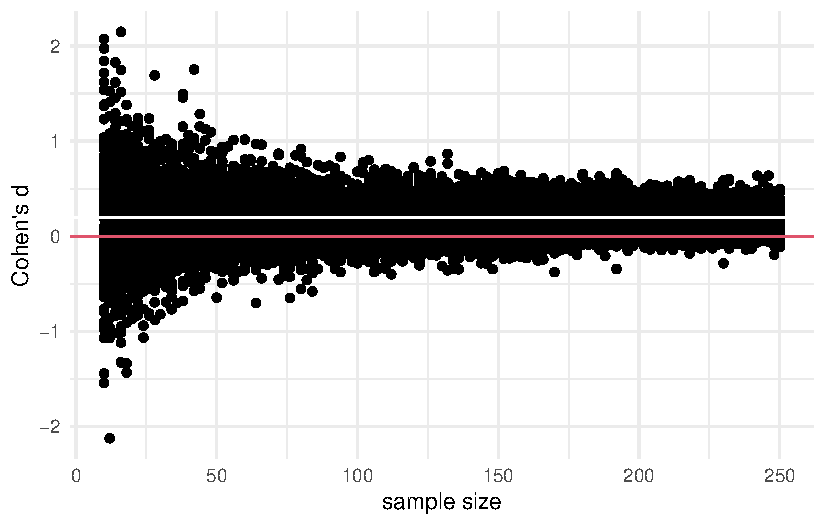
\includegraphics{07-power_effect_files/figure-pdf/fig-effectsizedispersion-1.pdf}

}

\caption{\label{fig-effectsizedispersion}Dispersion of estimated effect
size for data with a true mean dispersion of \(d=0.2\), for different
sample size.}

\end{figure}

\hypertarget{power}{%
\section{Power}\label{power}}

There are typically two uses to hypothesis test: either we want to show
it is not unreasonable to assume the null hypothesis (for example,
assuming equal variance), or else we want to show beyond reasonable
doubt that a difference or effect is significative: for example, one
could wish to demonstrate that a new website design (alternative
hypothesis) leads to a significant increase in sales relative to the
status quo (null hypothesis).

Our ability make discoveries depends on the power of the test: the
larger the power, the greater our ability to reject the null hypothesis
\(\mathscr{H}_0\) when the latter is false.

The \textbf{power of a test} is the probability of \textbf{correctly}
rejecting the null hypothesis \(\mathscr{H}_0\) when \(\mathscr{H}_0\)
is false, i.e., \begin{align*}
\mathsf{Pr}_a(\text{reject} \mathscr{H}_0)
\end{align*} Whereas the null alternative corresponds to a single value
(equality in mean), there are infinitely many alternatives\ldots{}
Depending on the alternative models, it is more or less easy to detect
that the null hypothesis is false and reject in favour of an
alternative. Power is thus a measure of our ability to detect real
effects. Different test statistics can give broadly similar conclusions
despite being based on different benchmark. Generally, however, there
will be a tradeoff between the number of assumptions we make about our
data or model (the fewer, the better) and the ability to draw
conclusions when there is truly something going on when the null
hypothesis is false.

\begin{figure}[ht!]

{\centering 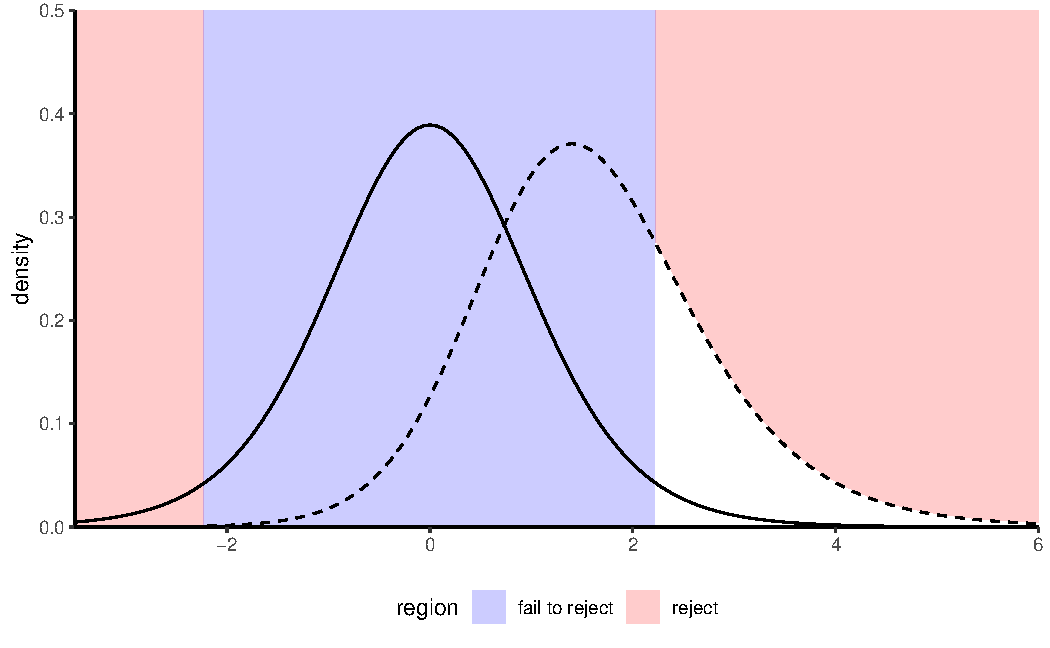
\includegraphics[width=0.8\textwidth,height=\textheight]{07-power_effect_files/figure-pdf/fig-power1-1.pdf}

}

\caption{\label{fig-power1}Comparison between null distribution (full
curve) and a specific alternative for a \emph{t}-test (dashed line). The
power corresponds to the area under the curve of the density of the
alternative distribution which is in the rejection area (in white).}

\end{figure}

\begin{figure}[ht!]

{\centering 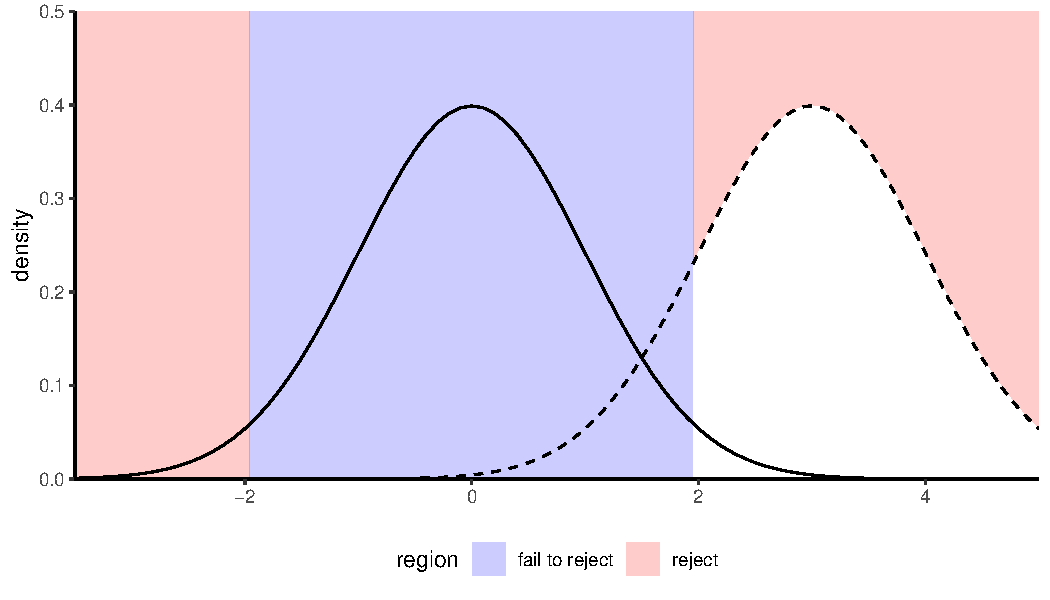
\includegraphics[width=0.8\textwidth,height=\textheight]{07-power_effect_files/figure-pdf/fig-power2-1.pdf}

}

\caption{\label{fig-power2}Increase in power due to an increase in the
mean difference between the null and alternative hypothesis. Power is
the area in the rejection region (in white) under the alternative
distribution (dashed): the latter is more shifted to the right relative
to the null distribution (full line).}

\end{figure}

\begin{figure}[ht!]

{\centering 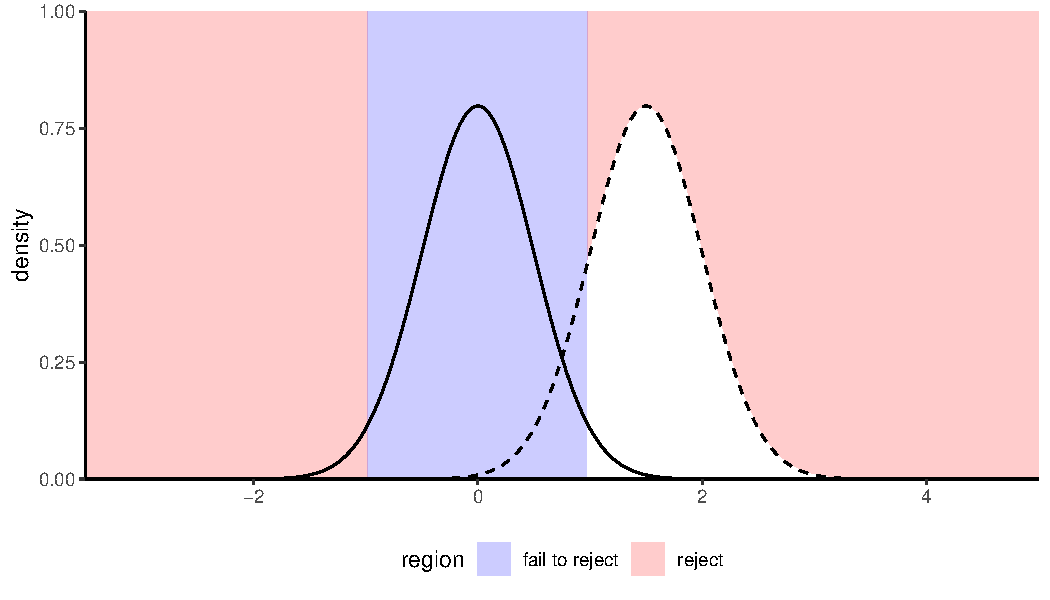
\includegraphics[width=0.8\textwidth,height=\textheight]{07-power_effect_files/figure-pdf/fig-power3-1.pdf}

}

\caption{\label{fig-power3}Increase of power due to an increase in the
sample size or a decrease of standard deviation of the population: the
null distribution (full line) is more concentrated. Power is given by
the area (white) under the curve of the alternative distribution
(dashed). In general, the null distribution changes with the sample
size.}

\end{figure}

We want to choose an experimental design and a test statistic that leads
to high power, so that this power is as close as possible to one. Under
various assumptions about the distribution of the original data, we can
derive optimal tests that are most powerful, but some of the power comes
from imposing more structure and these assumptions need not be satisfied
in practice.

Minimally, the power of the test should be \(\alpha\) because we reject
the null hypothesis \(\alpha\) fraction of the time even when
\(\mathscr{H}_0\) is true. Power depends on many criteria, notably

\begin{itemize}
\tightlist
\item
  the effect size: the bigger the difference between the postulated
  value for \(\theta_0\) under \(\mathscr{H}_0\) and the observed
  behaviour, the easier it is to detect departures from \(\theta_0\).
  (Figure~\ref{fig-power3}); it's easier to spot an elephant in a room
  than a mouse.
\item
  variability: the less noisy your data, the easier it is to assess that
  the observed differences are genuine, as Figure~\ref{fig-power2}
  shows;
\item
  the sample size: the more observation, the higher our ability to
  detect significative differences because the amount of evidence
  increases as we gather more observations.\footnote{Specifically, the
    standard error decreases with sample size \(n\) at a rate
    (typically) of \(n^{-1/2}\). The null distribution also becomes more
    concentrated as the sample size increase.} In experimental designs,
  the power also depends on how many observations are allocated to each
  group.\footnote{While the default is to assign an equal number to each
    subgroup, power may be maximized by specifying different sample size
    in each group if the variability of the measurement differ in these
    groups.}
\item
  the choice of test statistic: there is a plethora of possible
  statistics to choose from as a summary of the evidence against the
  null hypothesis. Choosing and designing statistics is usually best
  left out to statisticians, as there may be tradeoffs. For example,
  rank-based statistics discard information about the observed values of
  the response, focusing instead on their relative ranking. The
  resulting tests are typically less powerful, but they are also less
  sensible to model assumptions, model misspecification and outliers.
\end{itemize}

Changing the value of \(\alpha\) also has an impact on the power, since
larger values of \(\alpha\) move the cutoff towards the bulk of the
distribution. However, it entails a higher percentage of rejection also
when the alternative is false. Since the value of \(\alpha\) is fixed
beforehand to control the type I error (avoid judicial mistakes), it's
not a parameter we consider.

There is an intricate relation between effect size, power and sample
size. Journals and grant agencies oftentimes require an estimate of the
latter before funding a study, so one needs to ensure that the sample
size is large enough to pick-up effects of scientific interest (good
signal-to-noise), but also not overly large as to minimize time and
money and make an efficient allocation of resources. This is Goldilock's
principle, but having more never hurts.

If we run a pilot study to estimate the background level of noise and
the estimated effect, or if we wish to perform a replication study, we
will come up with a similar question in both cases: how many
participants are needed to reliably detect such a difference? Setting a
minimum value for the power (at least 80\%, but typically 90\% or 95\%
when feasible) ensures that the study is more reliable and ensures a
high chance of success of finding an effect of at least the size
specified. A power of 80\% ensures that, on average, 4 in 5 experiments
in which we study a phenomenon with the specified non-null effect size
should lead to rejecting the null hypothesis.

In order to better understand the interplay between power, effect size
and sample size, we consider a theoretical example. The purpose of
displaying the formula is to (hopefully) more transparently confirm some
of our intuitions about what leads to higher power. There are many
things that can influence the power:

\begin{itemize}
\tightlist
\item
  the experimental design: a blocking design or repeated measures tend
  to filter out some of the unwanted variability in the population, thus
  increasing power relative to a completely randomized design
\item
  the background variability \(\sigma\): the noise level is oftentimes
  intrinsic to the measurement. It depends on the phenomenon under
  study, but instrumentation and the choice of scale, etc. can have an
  impact. Running experiments in a controlled environment helps reduce
  this, but researchers typically have limited control on the
  variability inherent to each observation.
\item
  the sample size: as more data are gathered, information accumulates.
  The precision of measurements (e.g., differences in mean) is normally
  determined by the group with the smallest sample size, so
  (approximate) balancing increases power if the variance in each group
  is the same.
\item
  the size of the effect: the bigger the effect, the easier it is to
  accurately detect (it's easier to spot an elephant than a mouse hiding
  in a classroom).
\item
  the level of the test, \(\alpha\): if we increase the rejection
  region, we technically increase power when we run an experiment under
  an alternative regime. However, the level is oftentimes prespecified
  to avoid type I errors. We may consider multiplicity correction within
  the power function, such as Bonferonni's method, which is equivalent
  to reducing \(\alpha\).
\end{itemize}

\hypertarget{sec-power-oneway}{%
\subsection{Power for one-way ANOVA}\label{sec-power-oneway}}

To fix ideas, we consider the one-way analysis of variance model. In the
usual setup, we consider \(K\) experimental conditions with \(n_k\)
observations in group \(k\), whose population average we denote by
\(\mu_k\). We can parametrize the model in terms of the overall sample
average, \begin{align*}
\mu = \frac{1}{n}\sum_{j=1}^K\sum_{i=1}^{n_j} \mu_j = \frac{1}{n}\sum_{j=1}^K n_j \mu_j,
\end{align*} where \(n=n_1 + \cdots +n_K\) is the total sample size. The
\(F\)-statistic of the one-way ANOVA is \begin{align*}
F =  \frac{\text{between sum of squares}/(K-1)}{\text{within sum of squares}/(n-K)}
\end{align*} The null distribution is \(F(K-1, n-K)\). Our interest is
in understanding how the \emph{F}-statistic behaves under an
alternative.

During the construction, we stressed out that the denominator is an
estimator of \(\sigma^2\) under both the null and alternative. What
happens to the numerator? We can write the population average for the
between sum of square as \[
\mathsf{E}(\text{between sum of squares}) = \sigma^2\{(K-1) + \Delta\}.
\] where \[
\Delta = \dfrac{\sum_{j=1}^K n_j(\mu_j - \mu)^2}{\sigma^2} = nf^2.
\] and where \(f^2\) is the square of Cohen's \(f\). Under the null
hypothesis, all group means are equal and \(\mu_j=\mu\) for
\(j=1, \ldots, K\) and \(\Delta=0\), but if some groups have different
average the displacement will be non-zero. The greater \(\Delta\), the
further the mode (peak of the distribution) is from unity and the
greater the power.

Closer examination reveals that \(\Delta\) increases with \(n_j\)
(sample size) and with the true squared mean difference
\((\mu_j-\mu)^2\) increases effect size represented by the difference in
mean, but decreases as the observation variance increases.

Under the alternative, the distribution of the \(F\) statistic is a
noncentral Fisher distribution, denoted
\(\mathsf{F}(\nu_1, \nu_2, \Delta)\) with degrees of freedom \(\nu_1\)
and \(\nu_2\) and noncentrality parameter \(\Delta\).\footnote{Note that
  the \(F(\nu_1, \nu_2)\) distribution is indistinguishable from
  \(\chi^2(\nu_1)\) for \(\nu_2\) large. A similar result holds for
  tests with \(\chi^2\) null distributions.} To calculate the power of a
test, we need to single out a specific alternative hypothesis.

\begin{figure}[ht!]

{\centering 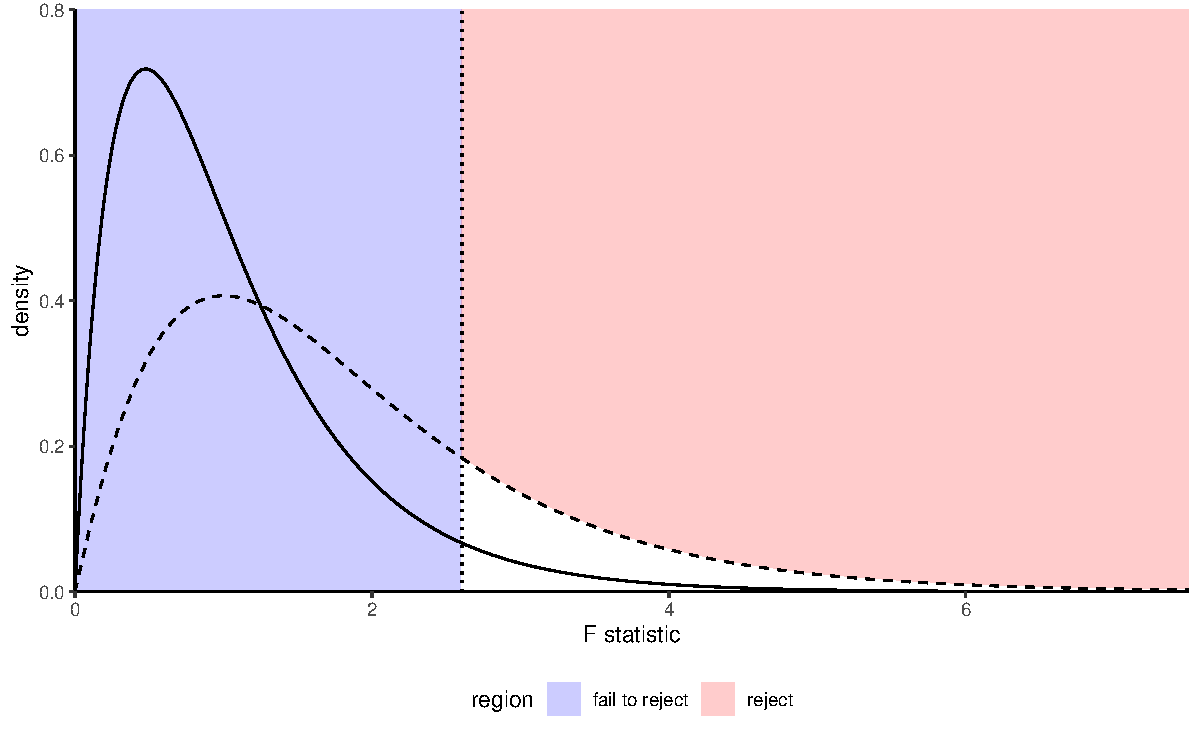
\includegraphics[width=0.8\textwidth,height=\textheight]{07-power_effect_files/figure-pdf/fig-powercurve-1.pdf}

}

\caption{\label{fig-powercurve}Density curves for the null distribution
(full line) and true distribution (dashed line) under noncentrality
parameter \(\Delta=3\). The area in white under the curve denotes the
power under this alternative.}

\end{figure}

The plot in Figure~\ref{fig-powercurve} shows the null (full line)
distribution and the true distribution (dashed line) for a particular
alternative. The noncentral \(\mathsf{F}\) is shifted to the right and
right skewed, so the mode (peak) is further away from 1.

Given a value of \(\Delta=nf^2\) and information about the effect of
interest (degrees of freedom of the effect and the residuals), we can
compute the tail probability as follows

\begin{enumerate}
\def\labelenumi{\arabic{enumi}.}
\tightlist
\item
  Compute the cutoff point: the value under \(\mathscr{H}_0\) that leads
  to rejection at level \(\alpha\)
\item
  Compute probability below the alternative curve, from the cutoff
  onwards.
\end{enumerate}

\begin{Shaded}
\begin{Highlighting}[]
\NormalTok{cutoff }\OtherTok{\textless{}{-}} \FunctionTok{qf}\NormalTok{(}\AttributeTok{p =} \DecValTok{1}\SpecialCharTok{{-}}\NormalTok{alpha, }\AttributeTok{df1 =}\NormalTok{ df1, }\AttributeTok{df2 =}\NormalTok{ df2)}
\FunctionTok{pf}\NormalTok{(}\AttributeTok{q =}\NormalTok{ cutoff,  }\AttributeTok{df1 =}\NormalTok{ df1, }\AttributeTok{df2 =}\NormalTok{ df2, }
    \AttributeTok{ncp =}\NormalTok{ Delta, }\AttributeTok{lower.tail =} \ConstantTok{FALSE}\NormalTok{)}
\end{Highlighting}
\end{Shaded}

\hypertarget{power-calculations}{%
\subsection{Power calculations}\label{power-calculations}}

In practice, a software will return these quantities and inform us about
the power. Note that these results are trustworthy provided the model
assumptions are met, otherwise they may be misleading.

The most difficult question when trying to estimate sample size for a
study is determining which value to use for the effect size. One could
opt for a value reported elsewhere for a similar scale to estimate the
variability and provide educated guesses for the mean differences.
Another option is to run a pilot study and use the resulting estimates
to inform about sensible values, perhaps using confidence intervals to
see the range of plausible effect sizes. Keep in mind the findings from
Figure~\ref{fig-effectsizedispersion}.

Reliance on estimated effect sizes reported in the literature is
debatable: many such effects are inflated as a result of the file-drawer
problem and, as such, can lead to unreasonably high expectations about
power.

The \texttt{WebPower} package in \textbf{R} offers a comprehensive
solution for conducting power studies, as does the free software
\href{https://www.psychologie.hhu.de/arbeitsgruppen/allgemeine-psychologie-und-arbeitspsychologie/gpower}{G*Power}.
We present a range of examples from a replication study: the following
quotes are taken from the \href{https://osf.io/ezcuj/}{Reproducibility
Project: Psychology}.

\begin{example}[Power calculation for between subject
ANOVA]\protect\hypertarget{exm-poweranova1}{}\label{exm-poweranova1}

The following extract of \href{https://osf.io/sd4uv/}{Jesse Chandler's
replication} concerns Study 4b by Janiszewski and Uy (2008), which
considers a \(2 \times 2\) between-subject ANOVA.

\begin{quote}
In Study 4a there are two effects of theoretical interest, a substantial
main effect of anchor precision that replicates the first three studies
and a small interaction (between precision and motivation within which
people can adjust) that is not central to the paper. The main effect of
anchor precision (effect size \(\eta^2_p=0.55\)) would require a sample
size of \(10\) for \(80\)\% power, \(12\) for \(90\)\% power, and \(14\)
for \(95\)\% power. The interaction (effect size \(\eta^2_p=0.11\))
would require a sample size of \(65\) for \(80\)\% power, \(87\) for
\(90\)\% power, and \(107\) for \(95\)\% power. There was also a
theoretically uninteresting main effect of motivation (people adjust
more when told to adjust more).
\end{quote}

In order to replicate, we must first convert estimates of \(\eta^2_p\)
to Cohen's \(f\), which is the input accepted by both \texttt{WebPower}
and G*Power. We compute the sample size for power 95\% for both the main
effect and the interaction: in practice, we would pick the smaller of
the two (or equivalently the larger resulting sample size estimate)
should we wish to replicate both findings.

\begin{Shaded}
\begin{Highlighting}[]
\NormalTok{f }\OtherTok{\textless{}{-}}\NormalTok{ effectsize}\SpecialCharTok{::}\FunctionTok{eta2\_to\_f}\NormalTok{(}\FloatTok{0.55}\NormalTok{) }\CommentTok{\# convert eta{-}squared to Cohen\textquotesingle{}s f}
\NormalTok{ng }\OtherTok{\textless{}{-}} \DecValTok{4} \CommentTok{\# number of groups for the ANOVA}
\FunctionTok{ceiling}\NormalTok{(WebPower}\SpecialCharTok{::}\FunctionTok{wp.kanova}\NormalTok{(}\AttributeTok{ndf =} \DecValTok{1}\NormalTok{, }\AttributeTok{ng =}\NormalTok{ ng, }\AttributeTok{f =}\NormalTok{ f, }\AttributeTok{power =} \FloatTok{0.95}\NormalTok{)}\SpecialCharTok{$}\NormalTok{n)}
\end{Highlighting}
\end{Shaded}

\begin{verbatim}
[1] 14
\end{verbatim}

\begin{Shaded}
\begin{Highlighting}[]
\NormalTok{f }\OtherTok{\textless{}{-}}\NormalTok{ effectsize}\SpecialCharTok{::}\FunctionTok{eta2\_to\_f}\NormalTok{(}\FloatTok{0.11}\NormalTok{)}
\FunctionTok{ceiling}\NormalTok{(WebPower}\SpecialCharTok{::}\FunctionTok{wp.kanova}\NormalTok{(}\AttributeTok{ndf =} \DecValTok{1}\NormalTok{, }\AttributeTok{ng =}\NormalTok{ ng, }\AttributeTok{f =}\NormalTok{ f, }\AttributeTok{power =} \FloatTok{0.95}\NormalTok{)}\SpecialCharTok{$}\NormalTok{n)}
\end{Highlighting}
\end{Shaded}

\begin{verbatim}
[1] 108
\end{verbatim}

We can see that the numbers match the calculations from the replication
(up to rounding).

\end{example}

\begin{example}[Power calculation for mixed
design]\protect\hypertarget{exm-power-within}{}\label{exm-power-within}

Repeated measures ANOVA have different characteristics from
between-subject design in that measurements are correlated, and we can
also provide correction for sphericity. These additional parameters need
to specified by users. In \texttt{WebPower}, the \texttt{wp.rmanova}
function. We need to specify the number of measurements per person, the
number of groups, the value \(\epsilon\) for the sphericity correction,
e.g., the output of Greenhouse--Geisser or Huynh--Feldt and the type of
effect for between-subject factor, within-subject factor or an
interaction between the two.

\begin{quote}
The result that is object of this replication is the interaction between
item strength (massed vs.~spaced presentation) and condition (directed
forgetting vs.~control). The dependent variable is the proportion of
correctly remembered items from the stimulus set (List 1). ``(..) The
interaction was significant, \(F(1,94)=4.97\), \(p <.05\),
\(\mathrm{MSE} =0.029\), \(\eta^2=0.05\), (\ldots)''. (p.~412). Power
analysis (G*Power (Version 3.1): ANOVA: Repeated measures,
within-between interaction with a zero correlation between the repeated
measures) indicated that sample sizes for \(80\)\%, \(90\)\% and
\(95\)\% power were respectively \(78\), \(102\) and \(126\).
\end{quote}

We are thus considering a \(2 \times 2\) within-between design. The
estimated effect size is \(\widehat{\eta}^2_p=0.05\), with Cohen's
\(f\), where the value is multiplied by a constant \(C\);
\href{https://webpower.psychstat.org/wiki/manual/power_of_rmanova}{see
the WebPower page} which depends on the number of groups, the number of
repeated measurements \(K\) and their correlation \(\rho\). For the
interaction, the correction factor is \(C = \sqrt{K/(1-\rho)}\): taking
\(K=2\) and \(\rho=0\), we get a Cohen's \(f\) of 0.23. We calculate the
sample size for a power of 90\% changing \(\rho\): if we change the
correlation in the calculation from zero to \(0.5\), we can see that
there is a significant decrease in the sample size.

\begin{Shaded}
\begin{Highlighting}[]
\NormalTok{f }\OtherTok{\textless{}{-}}\NormalTok{ effectsize}\SpecialCharTok{::}\FunctionTok{eta2\_to\_f}\NormalTok{(}\FloatTok{0.05}\NormalTok{) }\CommentTok{\# convert eta{-}squared to Cohen\textquotesingle{}s f}
\NormalTok{rho }\OtherTok{\textless{}{-}} \DecValTok{0} \CommentTok{\# correlation between measurements}
\NormalTok{K }\OtherTok{\textless{}{-}}\NormalTok{ 2L }\CommentTok{\# number of repeated measurements}
\FunctionTok{round}\NormalTok{(WebPower}\SpecialCharTok{::}\FunctionTok{wp.rmanova}\NormalTok{(}\AttributeTok{type =} \DecValTok{2}\NormalTok{, }\CommentTok{\# interaction }
                           \AttributeTok{nm =}\NormalTok{ K, }\CommentTok{\# number of measurement per subject}
                           \AttributeTok{ng =} \DecValTok{2}\NormalTok{, }\CommentTok{\# number of groups for between,}
                           \AttributeTok{f =}\NormalTok{ f}\SpecialCharTok{*}\FunctionTok{sqrt}\NormalTok{(K}\SpecialCharTok{/}\NormalTok{(}\DecValTok{1}\SpecialCharTok{{-}}\NormalTok{rho)), }\CommentTok{\# scaled effect size}
                           \AttributeTok{power =} \FloatTok{0.9}\NormalTok{)}\SpecialCharTok{$}\NormalTok{n) }\CommentTok{\# requested power}
\end{Highlighting}
\end{Shaded}

\begin{verbatim}
[1] 102
\end{verbatim}

\begin{figure}[ht!]

{\centering 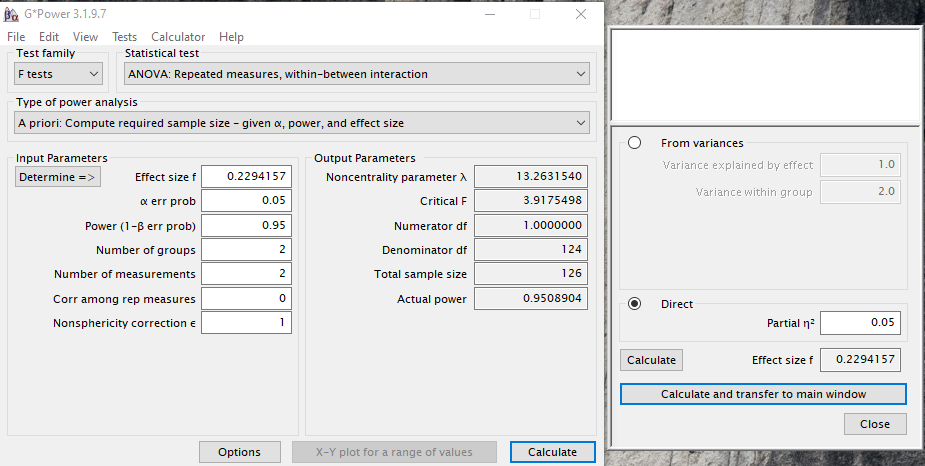
\includegraphics[width=1\textwidth,height=\textheight]{figures/GPower.png}

}

\caption{\label{fig-Gpower}Screenshot of G*Power for the calculation of
the sample size to replicate the interaction in a repeated measures
(within-between) analysis of variance.}

\end{figure}

\begin{figure}[ht!]

{\centering 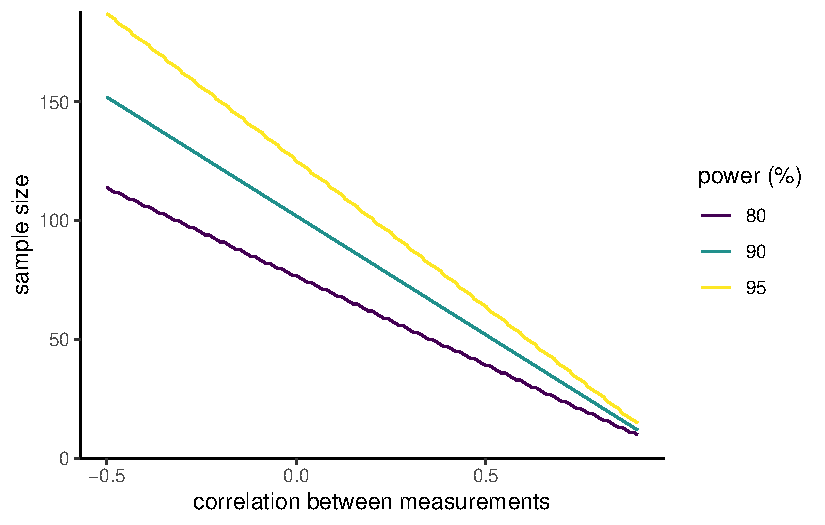
\includegraphics{07-power_effect_files/figure-pdf/fig-rmanova-1.pdf}

}

\caption{\label{fig-rmanova}Sample size requirement for a within-between
interaction in a two by two (within-between) ANOVa with an effect size
of \(\widehat{\eta}^2_p = 0.05\) as a function of correlation and power.
The staircase pattern is an artefact of rounding up to the nearest
integer.}

\end{figure}

We can see that the more correlated the response, the smaller sample
size requirement according to Figure~\ref{fig-rmanova}. Higher power
requirement leads to larger data collection efforts.

\end{example}

\begin{example}[Power calculation for a two sample
\(t\)-test]\protect\hypertarget{exm-power-ttest}{}\label{exm-power-ttest}

We consider a two-sample comparison, as these arise frequently from
contrasts. The replication wishes to replicate a study whose estimated
effect size was a Cohen's \(d\) of \(\widehat{d} = 0.451\). Using a
two-tailed test with a balanced sample and \(\alpha = 0.05\) type I
error rate, we obtain \(258\) participants. Note that some software, as
below, report the sample size by group so the total sample size is twice
the number reported.

\begin{Shaded}
\begin{Highlighting}[]
\DecValTok{2}\SpecialCharTok{*}\FunctionTok{ceiling}\NormalTok{(WebPower}\SpecialCharTok{::}\FunctionTok{wp.t}\NormalTok{(}
  \AttributeTok{type =} \StringTok{"two.sample"}\NormalTok{,}
  \AttributeTok{alternative =} \StringTok{"two.sided"}\NormalTok{,}
  \AttributeTok{d =} \FloatTok{0.451}\NormalTok{, }\CommentTok{\# Cohen\textquotesingle{}s f}
  \AttributeTok{power =} \FloatTok{0.95}\NormalTok{)}\SpecialCharTok{$}\NormalTok{n) }\CommentTok{\# power requirement}
\end{Highlighting}
\end{Shaded}

\begin{verbatim}
[1] 258
\end{verbatim}

The function also allows us to figure out the effect size one could
obtain for given power and fixed sample size, by replacing \texttt{d}
with the latter via arguments \texttt{n1} and \texttt{n2}.

\end{example}

\hypertarget{power-in-complex-designs}{%
\subsection{Power in complex designs}\label{power-in-complex-designs}}

In cases where an analytic derivations isn't possible, we can resort to
simulations to approximate the power. For a given alternative, we

\begin{itemize}
\tightlist
\item
  simulate repeatedly samples from the model from the hypothetical
  alternative world
\item
  we compute the test statistic for each of these new samples
\item
  we transform these to the associated \emph{p}-values based on the
  postulated null hypothesis.
\end{itemize}

At the end, we calculate the proportion of tests that lead to a
rejection of the null hypothesis at level \(\alpha\), namely the
percentage of \emph{p}-values smaller than \(\alpha\). We can vary the
sample size and see how many observations we need per group to achieve
the desired level of power.

\begin{tcolorbox}[enhanced jigsaw, colback=white, coltitle=black, rightrule=.15mm, left=2mm, bottomrule=.15mm, toprule=.15mm, titlerule=0mm, colframe=quarto-callout-important-color-frame, leftrule=.75mm, title=\textcolor{quarto-callout-important-color}{\faExclamation}\hspace{0.5em}{\textbf{Summary}}, breakable, arc=.35mm, colbacktitle=quarto-callout-important-color!10!white, opacitybacktitle=0.6, opacityback=0, toptitle=1mm, bottomtitle=1mm]

\begin{itemize}
\tightlist
\item
  Effect sizes are used to provide a standardized measure of the
  strength of a result, independent of the design and the sample size.
\item
  There are two classes: standardized differences and proportions of
  variance.
\item
  Multiple estimators exists: report the latter along with the software
  used to compute confidence intervals.
\item
  The adequate measure of variability to use for the effect size depends
  on the design: we normally include the variability of blocking factors
  and residual variance.
\item
  Given a design, we can deduce either the sample size, the power or the
  effect size from the other two metrics. This allows us to compute
  sample size for a study or replication.
\end{itemize}

\end{tcolorbox}

\bookmarksetup{startatroot}

\hypertarget{replication-crisis}{%
\chapter{Replication crisis}\label{replication-crisis}}

In recent years, many team efforts have performed so-called replications
of existing methodological papers to assess the robustness of their
findings. Perhaps unsurprisingly, many replications failed to yield
anything like what authors used to claim, or found much weaker findings.
This chapter examines some of the causes of this lack of replicability.

\begin{tcolorbox}[enhanced jigsaw, colback=white, coltitle=black, rightrule=.15mm, left=2mm, bottomrule=.15mm, toprule=.15mm, titlerule=0mm, colframe=quarto-callout-important-color-frame, leftrule=.75mm, title=\textcolor{quarto-callout-important-color}{\faExclamation}\hspace{0.5em}{Learning objectives}, breakable, arc=.35mm, colbacktitle=quarto-callout-important-color!10!white, opacitybacktitle=0.6, opacityback=0, toptitle=1mm, bottomtitle=1mm]

\begin{itemize}
\tightlist
\item
  Defining replicability and reproducibility.
\item
  Understanding the scale of the replication crisis.
\item
  Recognizing common statistical fallacies.
\item
  Listing strategies for enhancing reproducibility.
\end{itemize}

\end{tcolorbox}

We adopt the terminology of Claerbout and Karrenbach (1992): a study is
said to be \textbf{reproducible} if an external person with the same
data and enough indications about the procedure (for example, the code
and software versions, etc.) can obtain consistent results that match
those of a paper. A related scientific matter is \textbf{replicability},
which is the process by which new data are collected to test the same
hypothesis, potentially using different methodology. Reproducibility is
important because it enhances the credibility of one's work. Extensions
that deal with different analyses leading to the same conclusion are
described in
\href{\%5Bhttps://the-turing-way.netlify.app/reproducible-research/overview/overview-definitions.html\%5D}{The
Turing Way} and presented in Figure~\ref{fig-turingrepdo}.

\begin{figure}[ht!]

{\centering \includegraphics[width=0.8\textwidth,height=\textheight]{figures/turing_way.jpg}

}

\caption{\label{fig-turingrepdo}Definition of different dimensions of
reproducible research (from The Turing Way project, illustration by
Scriberia).}

\end{figure}

Why is reproducibility and replicability important? In a thought
provoking paper, Ioannidis (2005) claimed that most research findings
are wrong. The abstract of his paper stated

\begin{quote}
There is increasing concern that most current published research
findings are false. {[}\ldots{]} In this framework, a research finding
is less likely to be true when the studies conducted in a field are
smaller; when effect sizes are smaller; when there is a greater number
and lesser preselection of tested relationships; where there is greater
flexibility in designs, definitions, outcomes, and analytical modes;
when there is greater financial and other interest and prejudice; and
when more teams are involved in a scientific field in chase of
statistical significance.
\end{quote}

Since its publication, collaborative efforts have tried to assess the
scale of the problem by reanalysing data and trying to replicate the
findings of published research. For example, the ``Reproducibility
{[}sic{]} Project: Psychology'' (Nosek et al. 2015)

\begin{quote}
conducted replications of 100 experimental and correlational studies
published in three psychology journals using high powered designs and
original materials when available. Replication effects were half the
magnitude of original effects, representing a substantial decline.
Ninety seven percent of original studies had significant results. Thirty
six percent of replications had significant results; 47\% of original
effect sizes were in the 95\% confidence interval of the replication
effect size; 39\% of effects were subjectively rated to have replicated
the original result; and, if no bias in original results is assumed,
combining original and replication results left 68\% with significant
effects. {[}\ldots{]}
\end{quote}

A large share of findings in the review were not replicable or the
effects were much smaller than claimed, as shown by
\href{https://osf.io/447b3/}{Figure 2 from the study}. Such findings
show that the peer-review procedure is not foolproof: the
``publish-or-perish'' mindset in academia is leading many researchers to
try and achieve statistical significance at all costs to meet the 5\%
level criterion, whether involuntarily or not. This problem has many
names: \(p\)-hacking, harking or to paraphrase a
\href{https://en.wikipedia.org/wiki/The_Garden_of_Forking_Paths}{story
of Jorge Luis Borges}, the garden of forking paths. There are many
degrees of freedom in the analysis for researchers to refine their
hypothesis after viewing the data, conducting many unplanned comparisons
and reporting selected results.

\begin{figure}[ht!]

{\centering \includegraphics[width=0.7\textwidth,height=\textheight]{figures/RPP_psycho_repro.png}

}

\caption{\label{fig-repropvaluescorr}Figure 2 from Nosek et al. (2015),
showing scatterplot of effect sizes for the original and the replication
study by power, with rugs and density plots by significance at the 5\%
level.}

\end{figure}

Another problem is selective reporting. Because a large emphasis is
placed on statistical significance, many studies that find small effects
are never published, resulting in a gap. Figure~\ref{fig-reprozscores}
from Zwet and Cator (2021) shows \(z\)-scores obtained by transforming
confidence intervals reported in Barnett and Wren (2019). The authors
used data mining techniques to extract confidence intervals from
abstracts of nearly one million publication in Medline published between
1976 and 2019. If most experiments yielded no effect and were due to
natural variability, the \(z\)-scores should be normally distributed,
but Figure~\ref{fig-reprozscores} shows a big gap in the bell curve
between approximately \(-2\) and \(2\), indicative of selective
reporting. The fact that results that do not lead to \(p < 0.05\) are
not published is called the \textbf{file-drawer} problem.

\begin{figure}[ht!]

{\centering \includegraphics[width=0.6\textwidth,height=\textheight]{figures/vanZwet_Cator-zvalues.png}

}

\caption{\label{fig-reprozscores}Figure from Zwet and Cator (2021) based
on results of Barnett and Wren (2019); histogram of \(z\)-scores from
one million studies from Medline.}

\end{figure}

The ongoing debate surrounding the reproducibility crisis has sparked
dramatic changes in the academic landscape: to enhance the quality of
studies published, many journal now require authors to provide their
code and data, to pre-register their studies, etc. Teams lead effort
(e.g., the
\href{https://experimentaleconreplications.com/studies.html}{Experimental
Economics Replication Project}) try to replicate studies, with mitigated
success so far. This
\href{https://devonprice.medium.com/questionable-research-practices-ive-taken-part-in-754b74dcaa51}{inside
recollection} by a graduate student shows the extent of the problem.

This course will place a strong emphasis on identifying and avoiding
statistical fallacies and showcasing methods than enhance
reproducibility. How can reproducible research enhance your work? For
one thing, this workflow facilitates the publication of negative
research, forces researchers to think ahead of time (and receive
feedback). Reproducible research and data availability also leads to
additional citations and increased credibility as a scientist.

Among good practices are

\begin{itemize}
\tightlist
\item
  pre-registration of experiments and use of a logbook.
\item
  clear reporting of key aspects of the experiment (choice of metric,
  number of items in a Likert scale, etc.)
\item
  version control systems (e.g., Git) that track changes to files and
  records.
\item
  archival of raw data in a proper format with accompanying
  documentation.
\end{itemize}

Keeping a logbook and documenting your progress helps your
collaborators, reviewers and your future-self understand decisions which
may seem unclear and arbitrary in the future, even if they were the
result of a careful thought process at the time you made them. Given the
pervasiveness of the garden of forking paths, pre-registration helps you
prevents harking because it limits selective reporting and unplanned
tests, but it is not a panacea. Critics often object to pre-registration
claiming that it binds people. This is a misleading claim in my view:
pre-registration doesn't mean that you must stick with the plan exactly,
but merely requires you to explain what did not go as planned if
anything.

Version control keeps records of changes to your file and can help you
retrieve former versions if you make mistakes at some point.

\begin{figure}[ht!]

{\centering \includegraphics[width=0.6\textwidth,height=\textheight]{figures/reproducibility.png}

}

\caption{\label{fig-reprotweetexcelgenes}Tweet showing widespread
problems related to unintentional changes to raw data by software.}

\end{figure}

Archival of data helps to avoid unintentional and irreversible
manipulations of the original data, examples of which can have large
scale consequences as illustrated in
Figure~\ref{fig-reprotweetexcelgenes}, who report flaws in genetic
journals due to the automatic conversion of gene names to dates in
Excel. These problems are
\href{https://www.theguardian.com/politics/2020/oct/05/how-excel-may-have-caused-loss-of-16000-covid-tests-in-england}{far
from unique}. While sensitive data cannot be shared ``as is'' because of
confidentiality issues, in many instances the data can and should be
made available with a licence and a DOI to allow people to reuse it,
cite and credit your work.

To enforce reproducibility, many journals now have policy regarding
data, material and code availability. Some journals encourage such,
while the trend in recent years has been to enforce. For example, Nature
require the following to be reported in all published papers:

\begin{figure}[ht!]

{\centering \includegraphics[width=0.8\textwidth,height=\textheight]{figures/Nature_reporting_statistics.png}

}

\caption{Screenshot of the Nature Reporting summary for statistics,
reproduced under the CC BY 4.0 license.}

\end{figure}

\hypertarget{causes-of-the-replication-crisis}{%
\section{Causes of the replication
crisis}\label{causes-of-the-replication-crisis}}

Below are multiple (non-exclusive) explanations for the lack of
replication of study findings.

\hypertarget{the-garden-of-forking-paths}{%
\subsection{The garden of forking
paths}\label{the-garden-of-forking-paths}}

The garden of forking paths, named after a
\href{https://en.wikipedia.org/wiki/The_Garden_of_Forking_Paths}{novel
of Borges}, is a term coined by
\href{http://www.stat.columbia.edu/~gelman/research/unpublished/forking.pdf}{Andrew
Gelman} to refer to researchers' degrees of freedom. With vague
hypothesis and data collection rules, it is easy for the researcher to
adapt and interpret the conclusions in a way that fits his or her chosen
narratives. In the words of Gelman and Loken (2014)

\begin{quote}
Given a particular data set, it can seem entirely appropriate to look at
the data and construct reasonable rules for data exclusion, coding, and
analysis that can lead to statistical significance. In such a case,
researchers need to perform only one test, but that test is conditional
on the data.
\end{quote}

This user case is not accomodated by classical testing theory. Research
hypothesis are often formulated in a vague way, such that different
analysis methods, tests may be compatible.
\href{https://docs.iza.org/dp15476.pdf}{Abel et al.~(2022) recent
preprint} found that preregistration alone did not solve this problem,
but that publication bias in randomized control trial was alleviated by
publication of pre-analysis plans. This is directly related to the
garden of forking path.

\hypertarget{selective-reporting}{%
\subsection{Selective reporting}\label{selective-reporting}}

Also known as the file-drawer problem, selective reporting occurs
because publication of results that fail to reach statistical
significance (sic) are harder to publish. In much the same way as
multiple testing, if 20 researchers perform a study but only one of them
writes a paper and the result is a fluke, then this indicates. There are
widespread indications publication bias, as evidence by the distribution
of \(p\)-values reported in papers. A
\href{https://docs.iza.org/dp15478.pdf}{recent preprint of a study}
found the prevalance to be higher in online experiments such as Amazon
MTurks.

\emph{P}-hacking and the replication crisis has lead many leading
statisticians to advocate much more stringent cutoff criterion such as
\(p < 0.001\) instead of the usual \(p<0.05\) criterion as level for the
test. The level \(\alpha=5\)\% is essentially arbitrary and dates back
to Fisher (1926), who wrote

\begin{quote}
If one in twenty does not seem high enough odds, we may, if we prefer
it, draw the line at one in fifty or one in a hundred. Personally, the
writer prefers to set a low standard of significance at the 5 per cent
point, and ignore entirely all results which fails to reach this level.
\end{quote}

\begin{tcolorbox}[enhanced jigsaw, colback=white, coltitle=black, rightrule=.15mm, left=2mm, bottomrule=.15mm, toprule=.15mm, titlerule=0mm, colframe=quarto-callout-note-color-frame, leftrule=.75mm, title=\textcolor{quarto-callout-note-color}{\faInfo}\hspace{0.5em}{Thinking outside the box}, breakable, arc=.35mm, colbacktitle=quarto-callout-note-color!10!white, opacitybacktitle=0.6, opacityback=0, toptitle=1mm, bottomtitle=1mm]

Methods that pool together results, such as meta-analysis, are sensitive
to selective reporting. Why does it matter?

\end{tcolorbox}

\hypertarget{non-representative-samples}{%
\subsection{Non-representative
samples}\label{non-representative-samples}}

Many researchers opt for convenience samples by using online panels such
as Qualtrics, Amazon MTurks, etc. The quality of those observations is
at best dubious: ask yourself whether you would answer such as survey
for a small amount. Manipulation checks to ensure participants are
following, information is not completed by bots, a threshold for the
minimal time required to complete the study, etc. are necessary (but not
sufficient) conditions to ensure that the data are not rubbish.

A more important criticism is that the people who answer those surveys
are not representative of the population as a whole: sampling bias thus
plays an important role in the conclusions and, even if the summary
statistics are not too different from the general population, they may
exhibit different opinions, levels of skills, etc. than most.

\begin{figure}[ht!]

{\centering \includegraphics[width=0.65\textwidth,height=\textheight]{figures/samplingbias.jpg}

}

\caption{\label{fig-samplingbias}Sampling bias. Artwork by
\href{https://sketchplanations.com/sampling-bias}{Jonathan Hey
(Sketchplanations)} shared under the
\href{http://creativecommons.org/licenses/by-nc/4.0/}{CC BY-NC 4.0
license}.}

\end{figure}

The same can be said of panels of students recruited in universities
classes, who are more young, educated and perhaps may infer through
backward induction the purpose of the study and answer accordingly.

\hypertarget{summary-3}{%
\section{Summary}\label{summary-3}}

Operating in an open-science environment should be seen as an
opportunity to make better science, offer more opportunities to increase
your impact and increase the likelihood that your work gets published
regardless of whether the results turn out to be negative. It is the
\emph{right thing} to do and it increases the quality of research
produced, with collateral benefits because it forces researchers to
validate their methodology before, to double-check their data and their
analysis and to adopt good practice.

There are many platforms for preregistering studies and sharing
preanalysis plans, scripts and data, with different level of formality.
One such is the \href{https://researchbox.org/}{Research Box}.

\begin{tcolorbox}[enhanced jigsaw, colback=white, coltitle=black, rightrule=.15mm, left=2mm, bottomrule=.15mm, toprule=.15mm, titlerule=0mm, colframe=quarto-callout-tip-color-frame, leftrule=.75mm, title=\textcolor{quarto-callout-tip-color}{\faLightbulb}\hspace{0.5em}{Your turn}, breakable, arc=.35mm, colbacktitle=quarto-callout-tip-color!10!white, opacitybacktitle=0.6, opacityback=0, toptitle=1mm, bottomtitle=1mm]

Reflect on your workflow as applied researcher when designing and
undertaking experiments. Which practical aspects could you improve upon
to improve the reproducibility of your study?

\end{tcolorbox}

\bookmarksetup{startatroot}

\hypertarget{repeated-measures-and-multivariate-models}{%
\chapter{Repeated measures and multivariate
models}\label{repeated-measures-and-multivariate-models}}

So far, all experiments we have considered can be classified as
between-subject designs, meaning that each experimental unit was
assigned to a single experimental (sub)-condition. In many instances, it
may be possible to randomly assign multiple conditions to each
experimental unit. For example, an individual coming to a lab to perform
tasks in a virtual reality environment may be assigned to all
treatments. There is an obvious benefit to doing so, as the participants
can act as their own control group, leading to greater comparability
among treatment conditions.

For example, consider a study performed at Tech3Lab that looks at the
reaction time for people texting or talking on a cellphone while
walking. We may wish to determine whether disengagement is slower for
people texting, yet we may also postulate that some elderly people have
slower reflexes.

In a between-subjects design, subjects are \textbf{nested} within
experimental condition, as a subject can only be assigned a single
treatment. In a within-subjects designs, experimental factors and
subjects are \textbf{crossed}: it is possible to observed all
combination of subject and experimental conditions.

By including multiple conditions, we can filter out the effect due to
subject, much like with blocking: this leads to increased precision of
effect sizes and increased power (as we will see, hypothesis tests are
based on within-subject variability). Together, this translates into the
need to gather fewer observations or participants to detect a given
effect in the population and thus experiments are cheaper to run.

There are of course drawbacks to gathering repeated measures from
individuals. Because subjects are confronted with multiple tasks, there
may be carryover effects (when one task influences the response of the
subsequent ones, for example becoming better as manipulations go on),
period effects (fatigue, a decrease in acuity), and permanent changes in
the subject condition after a treatment or attrition (loss of subjects
over time).

To minimize potential biases, there are multiple strategies one can use.
Tasks are normally presented in random order among subjects to avoid
confounding, or using a balanced crossover design and include the period
and carryover effect in the statistical model via control variables so
as to better isolate the treatment effect. The experimenter should also
allow enough time between treatment conditions to reduce or eliminate
period or carryover effects and plan tasks accordingly.

If each subject is assigned to an experimental condition only once, one
good way to do this is via \textbf{counterbalancing}. We proceed as
follows: first, enumerate all possible orders of the condition and then
assign participants as equally as possible between conditions. For
example, with a single within-factor design with three conditions
\(A, B, C\), we have six possible orderings (either \(ABC\), \(ACB\),
\(BAC\), \(BCA\), \(CAB\) or \(CBA\)). Much like other forms of
randomization, this helps us remove confounding effects and let's us
estimate what is the average effect of task ordering on the response.

There are multiple approaches to handling repeated measures. The first
option is to take averages over experimental condition per subject and
treat them as additional blocking factors, but it may be necessary to
adjust the resulting statistics. The second approach consists in fitting
a multivariate model for the response and explicitly account for the
correlation, otherwise the null distribution commonly used are off and
so are the conclusions, as illustrated with the absurd comic displayed
in Figure~\ref{fig-xkcd2569}.

\begin{figure}[ht!]

{\centering \includegraphics[width=0.9\textwidth,height=\textheight]{figures/xkcd2533-slope_hypothesis_testing.png}

}

\caption{\label{fig-xkcd2569}xkcd comic
\href{https://xkcd.com/2533/}{2533 (Slope Hypothesis Testing) by Randall
Munroe}. Alt text: What? I can't hear-- I said, are you sure--; CAN YOU
PLEASE SPEAK--. Cartoon reprinted under the
\href{https://creativecommons.org/licenses/by-nc/2.5/}{CC BY-NC 2.5
license}.}

\end{figure}

Multivariate analysis of variance (MANOVA) leads to procedures that are
analogous to univariate analysis of variance, but we now need to
estimate correlation and variance parameters for each measurement
separately and there are multiple potential statistics that can be
defined for testing effects. While we can benefit from the correlation
and find differences that wouldn't be detected from univariate models,
the additional parameters to estimate lead to a loss of power. Finally,
the most popular method nowadays for handling repeated measures is to
fit a mixed model, with random effects accounting to subject-specific
characteristics. By doing so, we assume that the levels of a factor
(here the subject identifiers) form a random sample from a large
population. These models can be difficult to fit and one needs to take
great care in specifying the model.

\hypertarget{repeated-measures}{%
\section{Repeated measures}\label{repeated-measures}}

We introduce the concept of repeated measure and within-subject ANOVA
with an example.

\begin{example}[Happy
fakes]\protect\hypertarget{exm-happyfakes}{}\label{exm-happyfakes}

We consider an experiment conducted in a graduate course at HEC,
\emph{Information Technologies and Neuroscience}, in which PhD students
gathered electroencephalography (EEG) data. The project focused on human
perception of deepfake image created by a generative adversarial
network: Amirabdolahian and Ali-Adeeb (2021) expected the attitude
towards real and computer generated image of people smiling to change.

The response variable is the amplitude of a brain signal measured at 170
ms after the participant has been exposed to different faces. Repeated
measures were collected on 9 participants given in the database
\texttt{AA21}, who were expected to look at 120 faces. Not all
participants completed the full trial, as can be checked by looking at
the cross-tabs of the counts

\begin{Shaded}
\begin{Highlighting}[]
\FunctionTok{data}\NormalTok{(AA21, }\AttributeTok{package =} \StringTok{"hecedsm"}\NormalTok{)}
\FunctionTok{xtabs}\NormalTok{(}\SpecialCharTok{\textasciitilde{}}\NormalTok{stimulus }\SpecialCharTok{+}\NormalTok{ id, }\AttributeTok{data =}\NormalTok{ AA21)}
\end{Highlighting}
\end{Shaded}

\begin{verbatim}
        id
stimulus  1  2  3  4  5  6  7  8  9 10 11 12
    real 30 32 34 32 38 29 36 36 40 30 39 33
    GAN1 32 31 40 33 38 29 39 31 39 28 35 34
    GAN2 31 33 37 34 38 29 34 36 40 33 35 32
\end{verbatim}

The experimental manipulation is encoded in the \texttt{stimuli}, with
levels control (\texttt{real}) for real facial images, whereas the
others were generated using a generative adversarial network (GAN) with
be slightly smiling (\texttt{GAN1}) or extremely smiling
(\texttt{GAN2}); the latter looks more fake. While the presentation
order was randomized, the order of presentation of the faces within each
type is recorded using the \texttt{epoch} variable: this allows us to
measure the fatigue effect.

Since our research question is whether images generated from generative
adversarial networks trigger different reactions, we will be looking at
pairwise differences with the control.

\begin{figure}

\begin{minipage}[t]{0.33\linewidth}

{\centering 

\raisebox{-\height}{

\includegraphics{figures/face_real.png}

}

}

\subcaption{\label{fig-GANfaces-1}real}
\end{minipage}%
%
\begin{minipage}[t]{0.33\linewidth}

{\centering 

\raisebox{-\height}{

\includegraphics{figures/face_GAN_S.png}

}

}

\subcaption{\label{fig-GANfaces-2}slightly modified}
\end{minipage}%
%
\begin{minipage}[t]{0.33\linewidth}

{\centering 

\raisebox{-\height}{

\includegraphics{figures/face_GAN_E.png}

}

}

\subcaption{\label{fig-GANfaces-3}extremely modified}
\end{minipage}%

\caption{\label{fig-GANfaces}Examples of faces presented in
Amirabdolahian and Ali-Adeeb (2021).}

\end{figure}

We could first grouping the data and compute the average for each
experimental condition \texttt{stimulus} per participant and set
\texttt{id} as blocking factor. The analysis of variance table obtained
from \texttt{aov} would be correct, but would fail to account for
correlation.

The one-way analysis of variance with \(n_s\) subjects, each of which
was exposed to the \(n_a\) experimental conditions, can be written
\begin{align*}\underset{\text{response}\vphantom{l}}{Y_{ij}} = \underset{\text{global mean}}{\mu_{\vphantom{j}}} + \underset{\text{mean difference}}{\alpha_j} + \underset{\text{subject difference}}{s_{i\vphantom{j}}} + \underset{\text{error}\vphantom{l}}{\varepsilon_{ij}}
\end{align*}

\begin{Shaded}
\begin{Highlighting}[]
\CommentTok{\# Compute mean for each subject + }
\CommentTok{\# experimental condition subgroup}
\NormalTok{AA21\_m }\OtherTok{\textless{}{-}}\NormalTok{ AA21 }\SpecialCharTok{|\textgreater{}}
\NormalTok{  dplyr}\SpecialCharTok{::}\FunctionTok{group\_by}\NormalTok{(id, stimulus) }\SpecialCharTok{|\textgreater{}}
\NormalTok{  dplyr}\SpecialCharTok{::}\FunctionTok{summarize}\NormalTok{(}\AttributeTok{latency =} \FunctionTok{mean}\NormalTok{(latency))}
\CommentTok{\# Use aov for balanced sample}
\NormalTok{fixedmod }\OtherTok{\textless{}{-}} \FunctionTok{aov}\NormalTok{(}
\NormalTok{  latency }\SpecialCharTok{\textasciitilde{}}\NormalTok{ stimulus }\SpecialCharTok{+} \FunctionTok{Error}\NormalTok{(id}\SpecialCharTok{/}\NormalTok{stimulus), }
  \AttributeTok{data =}\NormalTok{ AA21\_m)}
\CommentTok{\# Print ANOVA table}
\FunctionTok{summary}\NormalTok{(fixedmod)}
\end{Highlighting}
\end{Shaded}

\begin{verbatim}

Error: id
          Df Sum Sq Mean Sq F value Pr(>F)
Residuals 11  187.8   17.07               

Error: id:stimulus
          Df Sum Sq Mean Sq F value Pr(>F)
stimulus   2   1.94  0.9704   0.496  0.615
Residuals 22  43.03  1.9557               
\end{verbatim}

Since the design is balanced after averaging, we can use \texttt{aov} in
\textbf{R}: we need to specify the subject identifier within
\texttt{Error} term. This approach has a drawback, as variance
components can be negative if the variability due to subject is
negligible. While \texttt{aov} is fast, it only works for simple
balanced designs.

\end{example}

\hypertarget{contrasts-1}{%
\subsection{Contrasts}\label{contrasts-1}}

With balanced data, the estimated marginal means coincide with the row
averages. If we have a single replication or the average for each
subject/condition, we could create a new column with the contrast and
then fit a model with an intercept-only (global mean) to check whether
the latter is zero. With 12 participants, we should thus expect our test
statistic to have 11 degrees of freedom, since one unit is spent on
estimating the mean parameter and we have 12 participants.

Unfortunately, the \texttt{emmeans} package analysis for object fitted
using \texttt{aov} will be incorrect: this can be seen by passing a
contrast vector and inspecting the degrees of freedom. The \texttt{afex}
package includes functionalities that are tailored for within-subject
and between-subjects and has an interface with \texttt{emmeans}.

\begin{Shaded}
\begin{Highlighting}[]
\NormalTok{afexmod }\OtherTok{\textless{}{-}}\NormalTok{ afex}\SpecialCharTok{::}\FunctionTok{aov\_ez}\NormalTok{(}
  \AttributeTok{id =} \StringTok{"id"}\NormalTok{,           }\CommentTok{\# subject id}
  \AttributeTok{dv =} \StringTok{"latency"}\NormalTok{,      }\CommentTok{\# response variable}
  \AttributeTok{within =} \StringTok{"stimulus"}\NormalTok{, }\CommentTok{\# within{-}subject factor}
  \AttributeTok{data =}\NormalTok{ AA21,}
  \AttributeTok{fun\_aggregate =}\NormalTok{ mean)}
\end{Highlighting}
\end{Shaded}

The \texttt{afex} package has different functions for computing the
within-subjects design and the \texttt{aov\_ez} specification, which
allow people to list within and between-subjects factor separately with
subject identifiers may be easier to understand. It also has an
argument, \texttt{fun\_aggregate}, to automatically average
replications.

\begin{Shaded}
\begin{Highlighting}[]
\CommentTok{\# Set up contrast vector}
\NormalTok{cont\_vec }\OtherTok{\textless{}{-}} \FunctionTok{list}\NormalTok{(}
  \StringTok{"real vs GAN"} \OtherTok{=} \FunctionTok{c}\NormalTok{(}\DecValTok{1}\NormalTok{, }\SpecialCharTok{{-}}\FloatTok{0.5}\NormalTok{, }\SpecialCharTok{{-}}\FloatTok{0.5}\NormalTok{))}
\FunctionTok{library}\NormalTok{(emmeans)}
\CommentTok{\# Correct output}
\NormalTok{afexmod }\SpecialCharTok{|\textgreater{}}
\NormalTok{  emmeans}\SpecialCharTok{::}\FunctionTok{emmeans}\NormalTok{(}
    \AttributeTok{spec =} \StringTok{"stimulus"}\NormalTok{, }
    \AttributeTok{contr =}\NormalTok{ cont\_vec)}
\end{Highlighting}
\end{Shaded}

\begin{verbatim}
$emmeans
 stimulus emmean    SE df lower.CL upper.CL
 real      -10.8 0.942 11    -12.8    -8.70
 GAN1      -10.8 0.651 11    -12.3    -9.40
 GAN2      -10.3 0.662 11    -11.8    -8.85

Confidence level used: 0.95 

$contrasts
 contrast    estimate    SE df t.ratio p.value
 real vs GAN   -0.202 0.552 11  -0.366  0.7213
\end{verbatim}

\begin{Shaded}
\begin{Highlighting}[]
\CommentTok{\# Incorrect output {-} }
\CommentTok{\# note the wrong degrees of freedom}
\NormalTok{fixedmod }\SpecialCharTok{|\textgreater{}} 
\NormalTok{  emmeans}\SpecialCharTok{::}\FunctionTok{emmeans}\NormalTok{(}
    \AttributeTok{spec =} \StringTok{"stimulus"}\NormalTok{, }
    \AttributeTok{contr =}\NormalTok{ cont\_vec)}
\end{Highlighting}
\end{Shaded}

\begin{verbatim}
Note: re-fitting model with sum-to-zero contrasts
\end{verbatim}

\begin{verbatim}
$emmeans
 stimulus emmean    SE   df lower.CL upper.CL
 real      -10.8 0.763 16.2    -12.4    -9.15
 GAN1      -10.8 0.763 16.2    -12.4    -9.21
 GAN2      -10.3 0.763 16.2    -11.9    -8.69

Warning: EMMs are biased unless design is perfectly balanced 
Confidence level used: 0.95 

$contrasts
 contrast    estimate    SE df t.ratio p.value
 real vs GAN   -0.202 0.494 22  -0.409  0.6867
\end{verbatim}

\hypertarget{sphericity-assumption}{%
\subsection{Sphericity assumption}\label{sphericity-assumption}}

The validity of the \(F\) statistic null distribution relies on the
model having the correct structure.

In repeated-measure analysis of variance, we assume again that each
measurement has the same variance. We equally require the correlation
between measurements of the same subject to be the same, an assumption
that corresponds to the so-called compound symmetry model.\footnote{Note
  that, with two measurements, there is a single correlation parameter
  to estimate and this assumption is irrelevant.}

What if the within-subject measurements have unequal variance or the
correlation between those responses differs?

Since we care only about differences in treatment, can get away with a
weaker assumption than compound symmetry (equicorrelation) by relying
instead on \emph{sphericity}, which holds if the variance of the
difference between treatment is constant. Sphericity is not a relevant
concept when there is only two measurements (as there is a single
correlation); we could check this by comparing the fit of a model with
an unstructured covariance (difference variances for each and
correlations for each pair of variable)

The most popular approach to handling correlation in tests is a
two-stage approach: first, check for sphericity (using, e.g., Mauchly's
test of sphericity). If the null hypothesis of sphericity is rejected,
one can use a correction for the \(F\) statistic by modifying the
parameters of the Fisher \(\mathsf{F}\) null distribution used as
benchmark.

An idea due to Box is to correct the degrees of freedom of the
\(\mathsf{F}(\nu_1, \nu_2)\) distribution by multiplying them by a
common factor \(\epsilon<1\) and use
\(\mathsf{F}(\epsilon\nu_1, \epsilon\nu_2)\) as null distribution
instead to benchmark our statistics and determine how extreme our
observed one is. Since the \(F\) statistic is a ratio of variances, the
\(\epsilon\) terms would cancel. Using the scaled \(\mathsf{F}\)
distribution leads to larger \(p\)-values, thus accounting for the
correlation.

There are three widely used corrections: Greenhouse--Geisser,
Huynh--Feldt and Box correction, which divides by \(\nu_1\) both degrees
of freedom and gives a very conservative option. The Huynh--Feldt method
is reported to be more powerful so should be preferred, but the
estimated value of \(\epsilon\) can be larger than 1.

Using the \texttt{afex} functions, we get the result for Mauchly's test
of sphericity and the \(p\) values from using either correction method

\begin{Shaded}
\begin{Highlighting}[]
\FunctionTok{summary}\NormalTok{(afexmod)}
\end{Highlighting}
\end{Shaded}

\begin{verbatim}

Univariate Type III Repeated-Measures ANOVA Assuming Sphericity

            Sum Sq num Df Error SS den Df  F value    Pr(>F)    
(Intercept) 4073.1      1  187.814     11 238.5554 8.373e-09 ***
stimulus       1.9      2   43.026     22   0.4962    0.6155    
---
Signif. codes:  0 '***' 0.001 '**' 0.01 '*' 0.05 '.' 0.1 ' ' 1


Mauchly Tests for Sphericity

         Test statistic p-value
stimulus        0.67814 0.14341


Greenhouse-Geisser and Huynh-Feldt Corrections
 for Departure from Sphericity

          GG eps Pr(>F[GG])
stimulus 0.75651     0.5667

            HF eps Pr(>F[HF])
stimulus 0.8514944  0.5872648
\end{verbatim}

\begin{example}[Visual
acuity]\protect\hypertarget{exm-visualacuity}{}\label{exm-visualacuity}

We consider a model with both within-subject and between-subject
factors. Data for a study on visual acuity of participants. The data
represent the number of words correctly detected at different font size;
interest is in effect of illusory contraction on detection. The mixed
analysis of variance includes the experimental factors
\texttt{adaptation} (2 levels, within), \texttt{fontsize} (4 levels,
within), \texttt{position} (5 levels, within) and visual \texttt{acuity}
(2 levels, between). There are a total of 1760 measurements for 44
participants in \texttt{LBJ17\_S1A}, balanced. The within-subject
factors give a total of 40 measurements (\(2 \times 4 \times 5\)) per
participant; all of these factors are crossed and we can estimate
interactions for them. The subjects are nested within visual acuity
groups, The participants were dichotomized in two groups based on their
visual acuity, obtained from preliminary checks, using a median split.

To fit the model, we rely on the \texttt{aov\_ez} function from
\texttt{afex}. By default, the latter includes all interactions.

\begin{Shaded}
\begin{Highlighting}[]
\NormalTok{LBJ\_mod }\OtherTok{\textless{}{-}}\NormalTok{ afex}\SpecialCharTok{::}\FunctionTok{aov\_ez}\NormalTok{(}
  \AttributeTok{id =} \StringTok{"id"}\NormalTok{,     }\CommentTok{\# subject id}
  \AttributeTok{dv =} \StringTok{"nerror"}\NormalTok{, }\CommentTok{\# response}
  \AttributeTok{between =} \StringTok{"acuity"}\NormalTok{,}
  \AttributeTok{within =} \FunctionTok{c}\NormalTok{(}\StringTok{"adaptation"}\NormalTok{,}
             \StringTok{"fontsize"}\NormalTok{, }
             \StringTok{"position"}\NormalTok{),}
  \AttributeTok{data =}\NormalTok{ hecedsm}\SpecialCharTok{::}\NormalTok{LBJ17\_S1A)}
\NormalTok{anova\_tbl }\OtherTok{\textless{}{-}} \FunctionTok{anova}\NormalTok{(LBJ\_mod,  }\CommentTok{\# model}
      \AttributeTok{correction =} \StringTok{"none"}\NormalTok{, }\CommentTok{\# no correction for sphericity}
      \AttributeTok{es =} \StringTok{"pes"}\NormalTok{) }
\CommentTok{\#partial eta{-}square for effect sizes (es)}
\end{Highlighting}
\end{Shaded}

\hypertarget{tbl-anova-fourway}{}
\begin{table}
\caption{\label{tbl-anova-fourway}Analysis of variance for the four-way model with partial effect sizes
(partial eta-square) }\tabularnewline

\centering
\begin{tabular}{lrrrrl}
\toprule
  & df1 & df2 & F & pes & p-value\\
\midrule
acuity & 1 & 42 & 30.8 & 0.42 & <0.001\\
adaptation & 1 & 42 & 7.8 & 0.16 & 0.008\\
acuity:adaptation & 1 & 42 & 12.7 & 0.23 & <0.001\\
fontsize & 3 & 126 & 1705.7 & 0.98 & <0.001\\
acuity:fontsize & 3 & 126 & 10.0 & 0.19 & <0.001\\
\addlinespace
position & 4 & 168 & 9.4 & 0.18 & <0.001\\
acuity:position & 4 & 168 & 4.2 & 0.09 & 0.003\\
adaptation:fontsize & 3 & 126 & 3.3 & 0.07 & 0.023\\
acuity:adaptation:fontsize & 3 & 126 & 7.0 & 0.14 & <0.001\\
adaptation:position & 4 & 168 & 0.6 & 0.01 & 0.662\\
\addlinespace
acuity:adaptation:position & 4 & 168 & 0.9 & 0.02 & 0.464\\
fontsize:position & 12 & 504 & 9.1 & 0.18 & <0.001\\
acuity:fontsize:position & 12 & 504 & 2.7 & 0.06 & 0.002\\
adaptation:fontsize:position & 12 & 504 & 0.5 & 0.01 & 0.907\\
acuity:adaptation:fontsize:position & 12 & 504 & 1.2 & 0.03 & 0.295\\
\bottomrule
\end{tabular}
\end{table}

This is the most complicated model we tested so far: there are four
experimental factor being manipulated at once, and all interactions of
order two, three and four are included!

The fourth order interaction isn't statistically significant: this means
that we can legitimately marginalize over and look at each of the four
three-way ANOVA designs in turn. We can also see that the third order
interaction \texttt{adaptation:fontsize:position} and
\texttt{acuity:adaptation:position} are not really meaningful.

The following paragraph is technical and can be skipped. One difficult
bit with designs including both within-subject and between-subject
factors is the degrees of freedom and the correct sum of square terms to
use to calculate the \(F\) statistics for each hypothesis of interest.
The correct setup is to use the next sum of square (and the associated
degrees of freedom) from this. For any main effect or interaction, we
count the number of instances of this particular (e.g., 10 for the
interaction between position and adaptation). We subtract the number of
mean parameter used to estimate means and differences in mean (1 global
mean, 4 means for position, 1 for adaptation), which gives \(4=10-6\)
degrees of freedom. Next, this term is compared to the mean square which
contains only subject (here via acuity levels, since subjects are nested
within acuity) and the corresponding variables; the correct mean square
is for \texttt{acuity:adaptation:position}. In the balanced design
setting, this can be formalized using Hasse diagram (Oehlert 2000).

We can produce an interaction plot to see what comes out: since we can't
draw in four dimensions, we map visual acuity and adaptation level to
panels with different colours for the position. The figure looks
different from the paper, seemingly because their \(y\)-axis is flipped.

\begin{figure}[ht!]

{\centering \includegraphics{09-repeated_files/figure-pdf/fig-LBJ-interactionplot-1.pdf}

}

\caption{\label{fig-LBJ-interactionplot}Interaction plot for visual
acuity levels.}

\end{figure}

\end{example}

\hypertarget{multivariate-analysis-of-variance}{%
\section{Multivariate analysis of
variance}\label{multivariate-analysis-of-variance}}

The second paradigm for modelling is to specify that the response from
each subject is in fact a multivariate object: we can combine all
measurements from a given individual in a vector \(\boldsymbol{Y}\). In
the example with the happy fakes, this would be the tuple of
measurements for (\texttt{real}, \texttt{GAN1}, \texttt{GAN2}).

The multivariate analysis of variance model is designed by assuming
observations follow a (multivariate) normal distribution with mean
vector \(\boldsymbol{\mu}_j\) in group \(j\) and common covariance
matrix \(\boldsymbol{\Sigma}\) and comparing means between groups. As in
univariate analysis of variance, the multivariate normal assumption
holds approximately by virtue of the central limit theorem in large
samples, but the convergence is slower and larger numbers are needed to
ensure this is valid.

The difference with the univariate approach is now that we will compare
a global mean vector \(\boldsymbol{\mu}\) between comparisons. In the
one-way analysis of variance model with an experimental factor having
\(K\) levels and a balanced sample \(n_g\) observations per group and
\(n=n_gK\) total observations, we assume that each group has average
\(\boldsymbol{\mu}_k\) \((k=1, \ldots, K)\), which we can estimate using
only the observations from that group. Under the null hypothesis, all
groups have the same mean, so the estimator is the overall mean
\(\boldsymbol{\mu}\) combining all \(n\) observations.

The statistic is obtained by decomposing the total variance around the
global mean into components due to the different factors and the
leftover variability. Because these equivalent to the sum of square
decomposition results in multiple matrices, there are multiple ways of
constructing test statistics. Wilk's \(\Lambda\) is the most popular
choice. Another common choice, which leads to a statistic giving lower
power but which is also more robust to departure from model assumptions
is Pillai's trace.

The MANOVA model assumes that the covariance matrices are the same
within each experimental condition. We can use Box's \(M\) statistic to
test the normality hypothesis.

\hypertarget{data-format}{%
\subsection{Data format}\label{data-format}}

With repeated measures, it is sometimes convenient to store measurements
associated to each experimental condition in different columns of a data
frame or spreadsheet, with lines containing participants identifiers.
Such data are said to be in \textbf{wide format}, since there are
multiple measurements in each row. While this format is suitable for
storate, many statistical routines will instead expect data to be in
\textbf{long format}, for which there is a single measurement per line.
Figure~\ref{fig-longvswide} illustrates the difference between the two
formats.

\begin{figure}[ht!]

{\centering \includegraphics[width=0.5\textwidth,height=\textheight]{figures/original-dfs-tidy.png}

}

\caption{\label{fig-longvswide}Long versus wide-format for data tables
(illustration by Garrick Aden-Buie).}

\end{figure}

Ideally, a data base in long format with repeated measures would also
include a column giving the order in which the treatments were assigned
to participants. This is necessary in order to test whether there are
fatigue or crossover effects, for example by plotting the residuals
after accounting for treatment subject by subject, ordered over time. We
could also perform formal tests by including time trends in the model
and checking whether the slope is significant.

Overall, the biggest difference with within-subject designs is that
observations are correlated whereas we assumed measurements were
independent until now. This needs to be explicitly accounted for, as
correlation has an important impact on testing as discussed
Section~\ref{sec-modelassumptionsindependence}: failing to account for
correlation leads to \(p\)-values that are much too low. To see why,
think about a stupid setting under which we duplicate every observation
in the database: the estimated marginal means will be the same, but the
variance will be halved despite the fact there is no additional
information. Intuitively, correlation reduces the amount of information
provided by each individual: if we have repeated measures from
participants, we expect the effective sample size to be anywhere between
the total number of subjects and the total number of observations.

\hypertarget{mathematical-complement}{%
\subsection{Mathematical complement}\label{mathematical-complement}}

This section is technical and can be omitted. Analogous to the
univariate case, we can decompose the variance estimator in terms of
within, between and total variance. Let \(\boldsymbol{Y}_{ik}\) denote
the response vector for the \(i\)th observation of group \(k\); then, we
can decompose the variance as \begin{align*} &
\underset{\text{total variance}}{\sum_{k=1}^K \sum_{i=1}^{n_g} (\boldsymbol{Y}_{ik} - \widehat{\boldsymbol{\mu}})(\boldsymbol{Y}_{ik} - \widehat{\boldsymbol{\mu}})^\top} \\\qquad &= \underset{\text{within variance}}{\sum_{k=1}^K \sum_{i=1}^{n_g} (\boldsymbol{Y}_{ik} - \widehat{\boldsymbol{\mu}}_k)(\boldsymbol{Y}_{ik} - \widehat{\boldsymbol{\mu}}_k)^\top} + \underset{\text{between variance}}{\sum_{k=1}^K n_g(\boldsymbol{\mu}_{k} - \widehat{\boldsymbol{\mu}})(\widehat{\boldsymbol{\mu}}_k - \widehat{\boldsymbol{\mu}})^\top}
\end{align*} defining covariance matrix estimators. If we write
\(\widehat{\boldsymbol{\Sigma}}_T,\)
\(\widehat{\boldsymbol{\Sigma}}_W\), and
\(\widehat{\boldsymbol{\Sigma}}_B\) for respectively the total, within
and between variance estimators, we can build a statistic from these
ingredients to see how much variability is induced by centering using a
common vector. When \(K>2\), there are multiple statistics that be
constructed, including

\begin{itemize}
\tightlist
\item
  Wilk's \(\Lambda\):
  \(|\widehat{\boldsymbol{\Sigma}}_W|/|\widehat{\boldsymbol{\Sigma}}_W + \widehat{\boldsymbol{\Sigma}}_B|\)
\item
  Roy's maximum root: the largest eigenvalue of
  \(\widehat{\boldsymbol{\Sigma}}_W^{-1}\widehat{\boldsymbol{\Sigma}}_B\)
\item
  Lawley--Hotelling trace:
  \(\mathrm{tr}(\widehat{\boldsymbol{\Sigma}}_W^{-1}\widehat{\boldsymbol{\Sigma}}_B)\)
\item
  Pillai's trace:
  \(\mathrm{tr}\left\{\widehat{\boldsymbol{\Sigma}}_B(\widehat{\boldsymbol{\Sigma}}_W +\widehat{\boldsymbol{\Sigma}}_B)^{-1}\right\}\).
\end{itemize}

All four criteria lead to equivalent statistics and the same
\(p\)-values if \(K=2\).

With a two-way balanced MANOVA, we can perform a similar decomposition
for each factor or interaction, with
\[\widehat{\boldsymbol{\Sigma}}_T = \widehat{\boldsymbol{\Sigma}}_A + \widehat{\boldsymbol{\Sigma}}_B + \widehat{\boldsymbol{\Sigma}}_{AB} + \widehat{\boldsymbol{\Sigma}}_W.\]

Wilk's \(\Lambda\) is based on taking the ratio of the determinant of
the within-variance and that of the sum of effect-variance plus
within-variance, e.g.,
\(|\widehat{\boldsymbol{\Sigma}}_{AB} + \widehat{\boldsymbol{\Sigma}}_W|\)
for the interaction term.

\hypertarget{model-fitting}{%
\subsection{Model fitting}\label{model-fitting}}

We can treat the within-subject responses as a vector of observations
and estimate the model using using multivariate linear regression.
Contrary to the univariate counterpart, the model explicitly models the
correlation between observations from the same subject.

In order to fit a model with a multivariate response, we first need to
pivot the data into wider format so as to have a matrix with rows for
the number of subjects and \(M\) columns for the number of response
variables.

Once the data are in a suitable format, we fit the multivariate model
with the \texttt{lm} function using the sum-to-zero constraints, here
imposed globally by changing the \texttt{contrasts} option. Syntax-wise,
the only difference with the univariate case is that the response on the
left of the tilde sign (\texttt{\textasciitilde{}}) is now a matrix
composed by binding together the vectors with the different responses.

\begin{example}[A multivariate take on ``Happy
fakes'']\protect\hypertarget{exm-happyfakemulti}{}\label{exm-happyfakemulti}

We use the data from Amirabdolahian and Ali-Adeeb (2021), but this time
treating the averaged repeated measures for the different stimulus as a
multivariate response. We first pivot the data to wide format, then fit
the multivariate linear model.

\begin{Shaded}
\begin{Highlighting}[]
\CommentTok{\# Pivot to wide format}
\NormalTok{AA21\_mw }\OtherTok{\textless{}{-}}\NormalTok{ AA21\_m }\SpecialCharTok{|\textgreater{}}
\NormalTok{  tidyr}\SpecialCharTok{::}\FunctionTok{pivot\_wider}\NormalTok{(}\AttributeTok{names\_from =}\NormalTok{ stimulus, }\CommentTok{\# within{-}subject factor labels}
                     \AttributeTok{values\_from =}\NormalTok{ latency) }\CommentTok{\# response measurements }
\CommentTok{\# Model with each variable with a different mean}
\CommentTok{\# Specify all columns with column bind }
\CommentTok{\# left of the \textasciitilde{}, following }
\FunctionTok{options}\NormalTok{(}\AttributeTok{contrasts =} \FunctionTok{c}\NormalTok{(}\StringTok{"contr.sum"}\NormalTok{, }\StringTok{"contr.poly"}\NormalTok{))}
\NormalTok{mlm }\OtherTok{\textless{}{-}} \FunctionTok{lm}\NormalTok{(}\FunctionTok{cbind}\NormalTok{(real, GAN1, GAN2) }\SpecialCharTok{\textasciitilde{}} \DecValTok{1}\NormalTok{,}
          \AttributeTok{data =}\NormalTok{ AA21\_mw)}
\end{Highlighting}
\end{Shaded}

Since the within-subject factor \texttt{stimulus} disappeared when we
consider the multivariate response, we only specify a global mean vector
\(\boldsymbol{\mu}\) via \texttt{\textasciitilde{}1}. In general, we
would add the between-subject factors to the right-hand side of the
equation. Our hypothesis of equal mean translates into the hypothesis
\(\boldsymbol{\mu} = \mu\boldsymbol{1}_3\), which can be imposed using a
call to \texttt{anova}. The output returns the statistic and
\(p\)-values including corrections for sphericity.

We can also use \texttt{emmeans} to set up post-hoc contrasts. Since we
have no variable, we need to set in \texttt{specs} the repeated measure
variable appearing on the left hand side of the formula; the latter is
labelled \texttt{rep.meas} by default.

\begin{Shaded}
\begin{Highlighting}[]
\CommentTok{\# Test the multivariate model against}
\CommentTok{\# equal mean (X = \textasciitilde{}1)}
\FunctionTok{anova}\NormalTok{(mlm, }\AttributeTok{X =} \SpecialCharTok{\textasciitilde{}}\DecValTok{1}\NormalTok{, }\AttributeTok{test =} \StringTok{"Spherical"}\NormalTok{)}
\end{Highlighting}
\end{Shaded}

\begin{verbatim}
Analysis of Variance Table


Contrasts orthogonal to
~1

Greenhouse-Geisser epsilon: 0.7565
Huynh-Feldt epsilon:        0.8515

            Df      F num Df den Df  Pr(>F)  G-G Pr  H-F Pr
(Intercept)  1 0.4962      2     22 0.61549 0.56666 0.58726
Residuals   11                                             
\end{verbatim}

\begin{Shaded}
\begin{Highlighting}[]
\CommentTok{\# Follow{-}up contrast comparisons}
\FunctionTok{library}\NormalTok{(emmeans)}
\NormalTok{emm\_mlm }\OtherTok{\textless{}{-}} \FunctionTok{emmeans}\NormalTok{(mlm, }\AttributeTok{specs =} \StringTok{"rep.meas"}\NormalTok{) }
\NormalTok{emm\_mlm }\SpecialCharTok{|\textgreater{}} \FunctionTok{contrast}\NormalTok{(}\AttributeTok{method =} \FunctionTok{list}\NormalTok{(}\FunctionTok{c}\NormalTok{(}\DecValTok{1}\NormalTok{,}\SpecialCharTok{{-}}\FloatTok{0.5}\NormalTok{,}\SpecialCharTok{{-}}\FloatTok{0.5}\NormalTok{)))}
\end{Highlighting}
\end{Shaded}

\begin{verbatim}
 contrast         estimate    SE df t.ratio p.value
 c(1, -0.5, -0.5)   -0.202 0.552 11  -0.366  0.7213
\end{verbatim}

We can check that the output is the same in this case as the
within-subject analysis of variance model fitted previously with the
\texttt{afex} package.

\end{example}

\begin{example}[Teaching to
read]\protect\hypertarget{exm-baumann-multi}{}\label{exm-baumann-multi}

We consider a between-subject repeated measure multivariate analysis of
variance model with the Baumann, Seifert-Kessell, and Jones (1992). The
data are balanced by experimental condition and they include the results
of three tests performed after the intervention: an error detection
task, an expanded comprehension monitoring questionnaire and a cloze
test. Note that the scale of the tests are different (16, 18 and 56).

We could obtain the estimated covariance matrix of the fitted model by
extracting the residuals \(Y_{ik} - \widehat{\mu}_k\) and computing the
empirical covariance. The results shows a strong dependence between
tests 1 and 3 (correlation of 0.39), but much weaker dependence with
test 2.

Let us compute the multivariate analysis of variance model

\begin{Shaded}
\begin{Highlighting}[]
\FunctionTok{data}\NormalTok{(BSJ92, }\AttributeTok{package =} \StringTok{"hecedsm"}\NormalTok{)}
\CommentTok{\# Force sum{-}to{-}zero parametrization}
\FunctionTok{options}\NormalTok{(}\AttributeTok{contrasts =} \FunctionTok{c}\NormalTok{(}\StringTok{"contr.sum"}\NormalTok{, }\StringTok{"contr.poly"}\NormalTok{))}
\CommentTok{\# Fit MANOVA model}
\NormalTok{mmod }\OtherTok{\textless{}{-}} \FunctionTok{lm}\NormalTok{(}
  \FunctionTok{cbind}\NormalTok{(posttest1, posttest2, posttest3) }\SpecialCharTok{\textasciitilde{}}\NormalTok{ group,}
   \AttributeTok{data =}\NormalTok{ BSJ92)}
\CommentTok{\# Calculate multivariate test}
\NormalTok{mtest }\OtherTok{\textless{}{-}}\NormalTok{ car}\SpecialCharTok{::}\FunctionTok{Anova}\NormalTok{(mmod, }\AttributeTok{test =} \StringTok{"Wilks"}\NormalTok{)}
\CommentTok{\# mtest}
\CommentTok{\# Get all statistics and univariate tests}
\FunctionTok{summary}\NormalTok{(car}\SpecialCharTok{::}\FunctionTok{Anova}\NormalTok{(mmod), }\AttributeTok{univariate =} \ConstantTok{TRUE}\NormalTok{)}
\end{Highlighting}
\end{Shaded}

\begin{verbatim}

Type II MANOVA Tests:

Sum of squares and products for error:
          posttest1  posttest2 posttest3
posttest1 640.50000   30.77273  498.3182
posttest2  30.77273  356.40909 -104.3636
posttest3 498.31818 -104.36364 2511.6818

------------------------------------------
 
Term: group 

Sum of squares and products for the hypothesis:
           posttest1 posttest2 posttest3
posttest1 108.121212  6.666667 190.60606
posttest2   6.666667 95.121212  56.65152
posttest3 190.606061 56.651515 357.30303

Multivariate Tests: group
                 Df test stat approx F num Df den Df     Pr(>F)    
Pillai            2 0.4082468 5.300509      6    124 6.7654e-05 ***
Wilks             2 0.6320200 5.243287      6    122 7.7744e-05 ***
Hotelling-Lawley  2 0.5185169 5.185169      6    120 8.9490e-05 ***
Roy               2 0.3184494 6.581288      3     62 0.00062058 ***
---
Signif. codes:  0 '***' 0.001 '**' 0.01 '*' 0.05 '.' 0.1 ' ' 1

 Type II Sums of Squares
          df posttest1 posttest2 posttest3
group      2    108.12    95.121     357.3
residuals 63    640.50   356.409    2511.7

 F-tests
      posttest1 posttest2 posttest3
group      5.32      8.41      4.48

 p-values
      posttest1  posttest2  posttest3 
group 0.00734676 0.00058043 0.01515115
\end{verbatim}

By default, we get Pillai's trace statistic. Here, there is clear
evidence of differences between groups of observations regardless of the
statistic being used.

We can compute effect size as before by passing the table, for example
using \texttt{eta\_squared(mtest)} to get the effect size of the
multivariate test, or simple the model to get the individual variable
effect sizes.

Having found a difference, one could in principle investigate for which
component of the response they are by performing univariate analysis of
variance and accounting for multiple testing using, e.g., Bonferroni's
correction. A more fruitful avenue if you are trying to discriminate is
to use descriptive discriminant analysis as a follow-up, which computes
the best fitting hyperplanes that separate groups.

\begin{Shaded}
\begin{Highlighting}[]
\NormalTok{MASS}\SpecialCharTok{::}\FunctionTok{lda}\NormalTok{(group }\SpecialCharTok{\textasciitilde{}}\NormalTok{ posttest1 }\SpecialCharTok{+}\NormalTok{ posttest2 }\SpecialCharTok{+}\NormalTok{ posttest3,}
          \AttributeTok{data =}\NormalTok{ BSJ92)}
\end{Highlighting}
\end{Shaded}

This amounts to compute the weights \(\boldsymbol{w}\) such, that,
computing \(\boldsymbol{w}^\top\boldsymbol{Y}\) creating a composite
score by adding up weighted components that leads to maximal separation
between groups. Figure~\ref{fig-lindiscrim} shows the new coordinates.

\begin{figure}[ht!]

{\centering \includegraphics[width=0.8\textwidth,height=\textheight]{09-repeated_files/figure-pdf/fig-lindiscrim-1.pdf}

}

\caption{\label{fig-lindiscrim}Scatterplot of observations projected
onto the linear discriminants for the post-experiment tests, by group.}

\end{figure}

Linear discriminant analysis is a topic on it's own that is beyond the
scope of the course.

\end{example}

\hypertarget{model-assumptions-1}{%
\subsection{Model assumptions}\label{model-assumptions-1}}

In addition to the usual model assumptions (independence of measurements
from different subjects, equal variance, additivity, etc.), the MANOVA
model adds two hypothesis that altogether determine how reliable our
\(p\)-values and conclusions are.

The first assumption is that of multivariate normality of the response.
The central limit theorem can be applied to a multivariate response, but
the sample size needed overall to reliably estimate the correlation and
variance is larger than in the univariate setting. This hypothesis can
be tested using the Shapiro-Wilk normality test (null hypothesis is that
of normality) by passing the residuals of the multivariate model. Such a
test can lead to rejection of the null hypothesis when specific
variables are far from normal, or when the dependence structure isn't
the one exhibited by a multivariate normal model. With decent sample
sizes (say \(n=50\) per group), this assumption isn't as important as
others.

\begin{Shaded}
\begin{Highlighting}[]
\CommentTok{\# Shapiro{-}Wilk normality test}
\CommentTok{\# Must transpose the residuals }
\CommentTok{\# to get a 3 by n matrix}
\NormalTok{mvnormtest}\SpecialCharTok{::}\FunctionTok{mshapiro.test}\NormalTok{(}\AttributeTok{U =} \FunctionTok{t}\NormalTok{(}\FunctionTok{resid}\NormalTok{(mmod)))}
\end{Highlighting}
\end{Shaded}

\begin{verbatim}

    Shapiro-Wilk normality test

data:  Z
W = 0.96464, p-value = 0.05678
\end{verbatim}

The second assumption is that the covariance matrix is the same for all
individuals, regardless of their experimental group assignment. We could
try checking whether a covariance model in each group: under
multivariate normal assumption, this leads to a test statistic called
Box's \(M\) test. Unfortunately, this test is quite sensitive to
departures from the multivariate normal assumption and, if the
\(p\)-value is small, it may have to do more with the normality than the
heterogeneity.

\begin{Shaded}
\begin{Highlighting}[]
\FunctionTok{with}\NormalTok{(BSJ92, }
\NormalTok{     biotools}\SpecialCharTok{::}\FunctionTok{boxM}\NormalTok{(}
       \AttributeTok{data =} \FunctionTok{cbind}\NormalTok{(posttest1, posttest2, posttest3),}
       \AttributeTok{grouping =}\NormalTok{ group))}
\end{Highlighting}
\end{Shaded}

\begin{verbatim}

    Box's M-test for Homogeneity of Covariance Matrices

data:  cbind(posttest1, posttest2, posttest3)
Chi-Sq (approx.) = 15.325, df = 12, p-value = 0.2241
\end{verbatim}

In our example, there is limited evidence against any of those model
assumptions. We should of course also check the assumptions of the
analysis of variance model for each of \texttt{postest1},
\texttt{posttest2} and \texttt{posttest3} in turn; such a check is left
as an exercice to the reader.

\hypertarget{power-and-effect-size}{%
\subsection{Power and effect size}\label{power-and-effect-size}}

Since all of the multivariate statistics can be transformed for a
comparison with a univariate \(\mathsf{F}\) distribution, we can
estimate partial effect size as before. The package \texttt{effectsize}
offers a measure of partial \(\widehat{\eta}^2\) for the multivariate
tests.\footnote{I must confess I haven't checked whether the output is
  sensical.}

Power calculations are beyond the reach of ordinary software as one
needs to specify the variance of each observation, their correlation and
their mean. Simulation is an obvious way for this kind of design to
obtain answers, but the free \textbf{G}\({}^{*}\)\textbf{Power} software
(Faul et al. 2007) also offers some tools. See also Läuter (1978) for
pairwise comparisons: to achieve a power of 80\%, we need the following
number of replicates per group \(j=1, \ldots, J\), which shows that the
number increases rapidly with the dimension of the response vector
\(p\). As usual, smaller effect sizes are more difficult to detect.

\begin{table}
\centering
\begin{tabular}[t]{l|r|r|r|r|r|r|r|r|r|r|r|r}
\hline
\multicolumn{1}{c|}{ } & \multicolumn{4}{c|}{3 groups} & \multicolumn{4}{c|}{4 groups} & \multicolumn{4}{c}{5 groups} \\
\cline{2-5} \cline{6-9} \cline{10-13}
effect size \textbackslash{} p & 2 & 4 & 6 & 8 & 2 & 4 & 6 & 8 & 2 & 4 & 6 & 8\\
\hline
very large & 13 & 16 & 18 & 21 & 14 & 18 & 21 & 23 & 16 & 21 & 24 & 27\\
\hline
large & 26 & 33 & 38 & 42 & 29 & 37 & 44 & 48 & 34 & 44 & 52 & 58\\
\hline
medium & 44 & 56 & 66 & 72 & 50 & 64 & 74 & 84 & 60 & 76 & 90 & 100\\
\hline
small & 98 & 125 & 145 & 160 & 115 & 145 & 165 & 185 & 135 & 170 & 200 & 230\\
\hline
\end{tabular}
\end{table}

\bookmarksetup{startatroot}

\hypertarget{introduction-to-mixed-models}{%
\chapter{Introduction to mixed
models}\label{introduction-to-mixed-models}}

This chapter considers tools for models with repeated measures from a
modern perspective, using random effects for modelling. This class of
model, called hierarchical models, multilevel models or mixed models in
simple scenarios, give us more flexibility to account for complex
scenarios in which there may be different sources of variability.

For example, consider a large-scale replication study about teaching
methods. We may have multiple labs partaking in a research program and
each has unique characteristics. Because of these, we can expect that
measurements collected within a lab will be correlated. At the same
time, we can have repeated mesures for participants in the study. One
can view this setup as a hierarchy, with within-subject factor within
subject within lab. In such settings, the old-school approach to
analysis of variance becomes difficult, if not impossible; it doesn't
easily account for the heterogeneity in the lab sample size and does not
let us estimate the variability within labs.

We begin our journey with the same setup as for repeated measures ANOVA
by considering one-way within-subject ANOVA model. We assign each
participant (subject) in the study to all of the experimental
treatments, in random order. If we have one experimental factor \(A\)
with \(n_a\) levels, the model is
\begin{align*}\underset{\text{response}\vphantom{l}}{Y_{ij}} = \underset{\text{global mean}}{\mu_{\vphantom{j}}} + \underset{\text{mean difference}}{\alpha_j} + \underset{\text{random effect for subject}}{S_{i\vphantom{j}}} + \underset{\text{error}\vphantom{l}}{\varepsilon_{ij}}.
\end{align*} In a random effect model, we assume that the subject effect
\(S_i\) is a random variable; we take
\(S_i \sim \mathsf{Normal}(0, \sigma^2_s)\) and the latter is assumed to
be independent of the noise
\(\varepsilon_{ij} \sim \mathsf{Normal}(0, \sigma^2_e)\). The model
parameters that we need to estimate are the global mean \(\mu\), the
mean differences \(\alpha_1, \ldots, \alpha_{n_a}\), the
subject-specific variability \(\sigma^2_s\) and the residual variability
\(\sigma^2_e\), with the sum-to-zero constraint
\(\alpha_1 + \cdots + \alpha_{n_a}=0\).

Inclusion of random effects introduces positive correlation between
measurements: specifically, the correlation between two observations
from the same subject will be
\(\rho=\sigma^2_s/(\sigma^2_s+\sigma^2_e)\) and zero otherwise. This
correlation structure is termed compound symmetry, since the correlation
between measurements, \(\rho\), is the same regardless of the order of
the observations. If there are multiple random effects, the dependence
structure will be more complicated.

In the repeated measure models, we need to first reduce measurements to
a single average per within-subject factor, then fit the model by
including the subject as a blocking factor. We are therefore considering
subjects as fixed effects by including them as blocking factors, and
estimate the mean effect for each subject: the value of \(\sigma^2_s\)
is estimated from the mean squared error of the subject term, but this
empirical estimate can be negative. By contrast, the mixed model
machinery will directly estimate the variance term, which will be
constrained to be strictly positive.

\hypertarget{fixed-vs-random-effects}{%
\section{Fixed vs random effects}\label{fixed-vs-random-effects}}

Mixed models include, by definition, both \textbf{random} and
\textbf{fixed} effects. Fixed effects are model parameters corresponding
to overall average or difference in means for the experimental
conditions. These are the terms for which we want to perform hypothesis
tests and compute contrasts. So far, we have only considered models with
fixed effects.

Random effects, on the other hand, assumes that the treatments are
random samples from a population of interest. If we gathered another
sample, we would be looking at a new set of treatments. Random effects
model the variability arising from the sampling of that population and
focuses on variance and correlation parameters. Addition of random
effects does not impact the population mean, but induces variability and
correlation within subject. There is no consensual definition, but
Gelman (2005) lists a handful:

\begin{quote}
When a sample exhausts the population, the corresponding variable is
fixed; when the sample is a small (i.e., negligible) part of the
population the corresponding variable is random {[}Green and Tukey
(1960){]}.
\end{quote}

\begin{quote}
Effects are fixed if they are interesting in themselves or random if
there is interest in the underlying population (e.g., Searle, Casella
and McCulloch {[}(1992), Section 1.4{]})
\end{quote}

In terms of estimation, fixed effect terms are mean parameters, while
all random effects will be obtained from variance and correlation
parameters. In the repeated measure approach with fixed effects and
blocking, we would estimate the average for each subject despite the
fact that this quantity is of no interest. Estimating a mean with only a
handful of measurements is a risky business and the estimated effects
are sensitive to outliers.

Random effects would proceed to directly estimate the variability
arising from different subjects. We can still get predictions for the
subject-specific effect, but this prediction will be shrunk toward the
global mean for that particular treatment category. As we gather more
data about the subjects, the predictions will become closer to the fixed
effect estimates when the number of observations per subject or group
increases, but these prediction can deviate from mean estimates in the
case where there are few measurements per subject.

Oehlert (2000) identifies the following step to perform a mixed model

\begin{enumerate}
\def\labelenumi{\arabic{enumi}.}
\tightlist
\item
  Identify sources of variation
\item
  Identify whether factors are crossed or nested
\item
  Determine whether factors should be fixed or random
\item
  Figure out which interactions can exist and whether they can be
  fitted.
\end{enumerate}

Sources of variations are all factors (including identifiers) which
could influence the response.

We say to factors are nested (\(A\) within \(B\)) when one can only
coexist within the levels of the other: this has implications, for we
cannot have interaction between the two. In between-subject experiments,
subjects are nested in between-subject factors and the experimental
factors are crossed, meaning we can assign an experimental unit or a
subject to each factor combination. Interactions can occur for the
between-subject factors, although we need participants in each
subcategory to estimate them.

\begin{example}[Temporal distancing in peace
prospects]\protect\hypertarget{exm-tempdist}{}\label{exm-tempdist}

We consider a three-way mixed design from Study 5 of Halevy and Berson
(2022). The research studied how temporal distance impacted the
prospects of peace by presenting participants with a fictional scenario
in which two tribes in a fictional country, Velvetia, where either at
war or peace and asking what they think the outcome would be in the near
and distance future. Participants rated the likeliness using a Likert
scale ranging from extremely unlikely (1) to extremely likely (7) for
the question

\begin{quote}
There is currently {[}war/peace{]} between the two tribes in Velvetia.
Thinking about {[}next year/in 20 years{]}, how likely is it that there
will be {[}war/peace{]} in Velvetia?
\end{quote}

Each participant was assigned to a single combination of the current
state \texttt{curstate} and the predicted outcome \texttt{predout} and
answered the question for both temporal horizon, \texttt{tempdist}. A
rapid examination shows that we have a complete design: there are
participants assigned to each subcategory of the between-subject
factors.

\begin{Shaded}
\begin{Highlighting}[]
\FunctionTok{data}\NormalTok{(HB22\_S5, }\AttributeTok{package =} \StringTok{"hecedsm"}\NormalTok{)}
\FunctionTok{xtabs}\NormalTok{(}\SpecialCharTok{\textasciitilde{}}\NormalTok{ curstate }\SpecialCharTok{+}\NormalTok{ predout, }\AttributeTok{data =}\NormalTok{ HB22\_S5)}
\end{Highlighting}
\end{Shaded}

\begin{verbatim}
        predout
curstate peace war
   peace   148 164
   war     118 124
\end{verbatim}

\begin{enumerate}
\def\labelenumi{\arabic{enumi}.}
\tightlist
\item
  The sources of variation are participants \texttt{id}, between-subject
  factors \texttt{predout} and \texttt{curstate} and within-subjects
  factor \texttt{tempdist}.
\item
  Between subject factors \texttt{predout} and \texttt{curstate} are
  crossed, whereas \texttt{tempdist} is nested within \texttt{id}.
\item
  \texttt{id} is random, whereas \texttt{predout}, \texttt{curstate} and
  \texttt{tempdist} are fixed effects
\item
  We can have interactions between the three experimental factors
  \texttt{predout}, \texttt{curstate} and \texttt{tempdist} since the
  database contains instances of both of the former together, and since
  each person gets two \texttt{tempdist} levels. However, no interaction
  are possible between \texttt{id} and \texttt{tempdist} (due to lack of
  replication), or between between-subject factors and identifiers.
\end{enumerate}

With data in long format, meaning each line contains a single response
and characteristics are repeated per row, the software will
automatically capture the random effect. We can fit the equivalent of
the repeated measure mixed ANOVA using a linear mixed model in
\textbf{R}, by simply specifying a random intercept for the participant
\texttt{id}. The full model with the three-way interaction includes
eight components for the mean and two variant component (residual
variance, and subject-specific variance).

\begin{Shaded}
\begin{Highlighting}[]
\CommentTok{\# In R, two packages offer linear mixed model fit via (RE)ML}
\CommentTok{\# lme4 is more modern (and reliable?), but does not allow for unequal variant}
\NormalTok{lme4}\SpecialCharTok{::}\FunctionTok{lmer}\NormalTok{(likelihood }\SpecialCharTok{\textasciitilde{}}\NormalTok{ curstate}\SpecialCharTok{*}\NormalTok{predout}\SpecialCharTok{*}\NormalTok{tempdist }\SpecialCharTok{+}\NormalTok{ (}\DecValTok{1} \SpecialCharTok{|}\NormalTok{ id),}
     \AttributeTok{data =}\NormalTok{ HB22\_S5)}
\end{Highlighting}
\end{Shaded}

\begin{verbatim}
Linear mixed model fit by REML ['lmerMod']
Formula: likelihood ~ curstate * predout * tempdist + (1 | id)
   Data: HB22_S5
REML criterion at convergence: 1933.813
Random effects:
 Groups   Name        Std.Dev.
 id       (Intercept) 0.8524  
 Residual             1.1436  
Number of obs: 554, groups:  id, 277
Fixed Effects:
                        (Intercept)                          curstatewar  
                              5.581                               -2.886  
                         predoutwar                         tempdist20yr  
                             -2.337                               -1.068  
             curstatewar:predoutwar             curstatewar:tempdist20yr  
                              5.142                                3.508  
            predoutwar:tempdist20yr  curstatewar:predoutwar:tempdist20yr  
                              2.775                               -6.554  
\end{verbatim}

\begin{Shaded}
\begin{Highlighting}[]
\CommentTok{\#  Note that in \textasciigrave{}lme4\textasciigrave{} package, the random effects are specified inside parenthesis}
\CommentTok{\# nlme offers the possibility to acount for unequal variance per group}
\CommentTok{\# Random effects are specified in \textasciigrave{}random\textasciigrave{} with formula notation, and a | to indicate}
\NormalTok{nlme}\SpecialCharTok{::}\FunctionTok{lme}\NormalTok{(likelihood }\SpecialCharTok{\textasciitilde{}}\NormalTok{ curstate}\SpecialCharTok{*}\NormalTok{predout}\SpecialCharTok{*}\NormalTok{tempdist, }\AttributeTok{random =} \SpecialCharTok{\textasciitilde{}} \DecValTok{1} \SpecialCharTok{|}\NormalTok{ id, }\AttributeTok{data =}\NormalTok{ HB22\_S5)}
\end{Highlighting}
\end{Shaded}

\begin{verbatim}
Linear mixed-effects model fit by REML
  Data: HB22_S5 
  Log-restricted-likelihood: -966.9064
  Fixed: likelihood ~ curstate * predout * tempdist 
                        (Intercept)                         curstatewar 
                           5.581081                           -2.886166 
                         predoutwar                        tempdist20yr 
                          -2.337179                           -1.067568 
             curstatewar:predoutwar            curstatewar:tempdist20yr 
                           5.142263                            3.508246 
            predoutwar:tempdist20yr curstatewar:predoutwar:tempdist20yr 
                           2.774885                           -6.554272 

Random effects:
 Formula: ~1 | id
        (Intercept) Residual
StdDev:   0.8523522 1.143597

Number of Observations: 554
Number of Groups: 277 
\end{verbatim}

\end{example}

\begin{example}[Happy fakes,
remixed]\protect\hypertarget{exm-happy-fakes-revisited}{}\label{exm-happy-fakes-revisited}

We consider again the experiment of Amirabdolahian and Ali-Adeeb (2021)
on smiling fakes and the emotion, this time from a pure mixed model
perspective. This means we can simply keep all observations and model
them accordingly. To fit the model, identifiers of subjects must be
declared as factors (categorical variables). If we have repeated
measurements of the within-subject factor, we may consider adding a
random effect for the interaction between the subject and the
within-subject factor.

\begin{figure}[ht!]

{\centering \includegraphics[width=0.8\textwidth,height=\textheight]{10-mixed_files/figure-pdf/fig-aafulldat-1.pdf}

}

\caption{\label{fig-aafulldat}Jittered scatterplot of individual
measurements per participant and stimulus type.}

\end{figure}

Figure~\ref{fig-aafulldat} shows the raw measurements, including what
are notable outliers that may be due to data acquisition problems or
instrumental manipulations. Since the experiment was performed in a
non-controlled setting (pandemic) with different apparatus and everyone
acting as their own technician, it is unsurprising that the
signal-to-noise ratio is quite small. We will exclude here (rather
arbitrarily) measurements below a latency of minus 40.

\begin{Shaded}
\begin{Highlighting}[]
\FunctionTok{library}\NormalTok{(lmerTest) }\CommentTok{\# Package to fit and tests for mixed models}
\FunctionTok{options}\NormalTok{(}\AttributeTok{contrasts =} \FunctionTok{c}\NormalTok{(}\StringTok{"contr.sum"}\NormalTok{, }\StringTok{"contr.poly"}\NormalTok{))}
\NormalTok{mixedmod }\OtherTok{\textless{}{-}} \FunctionTok{lmer}\NormalTok{(}
\NormalTok{  latency }\SpecialCharTok{\textasciitilde{}}\NormalTok{ stimulus }\SpecialCharTok{+} 
\NormalTok{    (}\DecValTok{1} \SpecialCharTok{|}\NormalTok{ id) }\SpecialCharTok{+} \CommentTok{\# random effect for subject}
\NormalTok{    (}\DecValTok{1} \SpecialCharTok{|}\NormalTok{ id}\SpecialCharTok{:}\NormalTok{stimulus), }\CommentTok{\# interaction id and stimuluss}
  \CommentTok{\# random effect for interaction }
  \AttributeTok{data =}\NormalTok{ hecedsm}\SpecialCharTok{::}\NormalTok{AA21 }\SpecialCharTok{|\textgreater{}} \CommentTok{\#remove outliers}
\NormalTok{    dplyr}\SpecialCharTok{::}\FunctionTok{filter}\NormalTok{(latency }\SpecialCharTok{\textgreater{}} \SpecialCharTok{{-}}\DecValTok{40}\NormalTok{))}
\CommentTok{\# Output parameter estimates}
\FunctionTok{print}\NormalTok{(mixedmod)}
\end{Highlighting}
\end{Shaded}

\begin{verbatim}
Linear mixed model fit by REML ['lmerModLmerTest']
Formula: latency ~ stimulus + (1 | id) + (1 | id:stimulus)
   Data: dplyr::filter(hecedsm::AA21, latency > -40)
REML criterion at convergence: 8007.913
Random effects:
 Groups      Name        Std.Dev.
 id:stimulus (Intercept) 0.7371  
 id          (Intercept) 2.2679  
 Residual                6.2235  
Number of obs: 1227, groups:  id:stimulus, 36; id, 12
Fixed Effects:
(Intercept)    stimulus1    stimulus2  
   -10.5374      -0.2529      -0.1394  
\end{verbatim}

The model includes a fixed effect for stimulus, and variance terms for
\texttt{stimulus} (nested within \texttt{id}) and subject identifier
\texttt{id}. We see that there is quite a bit of heterogeneity between
participants and per stimulus participant pair, albeit less so for the
interaction. All estimated variance terms are rather large. We can also
look globally at the statistical evidence for the difference between the
various stimuli.

\begin{Shaded}
\begin{Highlighting}[]
\CommentTok{\# Global effect of different faces}
\CommentTok{\# ANOVA here is type III effects }
\CommentTok{\# computed from the \textquotesingle{}lmerTest\textquotesingle{} package}
\FunctionTok{anova}\NormalTok{(mixedmod)}
\end{Highlighting}
\end{Shaded}

\begin{verbatim}
Type III Analysis of Variance Table with Satterthwaite's method
         Sum Sq Mean Sq NumDF  DenDF F value Pr(>F)
stimulus  65.62   32.81     2 23.337  0.8471 0.4414
\end{verbatim}

The global \(F\) test of significance for stimulus is based on an
approximation that accounts for the correlation between observations;
the denominator degrees of freedom for the approximate \(F\) statistic
are based on Satterthwaite's method. There is again no evidence of
differences between experimental conditions. This is rather unsurprising
if we look at the raw data in Figure~\ref{fig-aafulldat}.

\end{example}

\begin{example}[Verbalization and
memorization]\protect\hypertarget{exm-verbalization-memorization}{}\label{exm-verbalization-memorization}

We consider a replication study of Elliott et al. (2021), which studied
verbalization and verbalization of kids aged 5, 6, 7 and 10. The
replication was performed in 17 different school labs, adapting a
protocol of Flavell, Beach, and Chinsky (1966), with an overall sample
of 977 child partaking in the experiment.

Each participant was assigned to three tasks (\texttt{timing}):
\texttt{delayed} recall with 15 seconds wait, or \texttt{immediate}, and
finally a naming task (\texttt{point-and-name}). The \texttt{taskorder}
variable records the order in which these were presented: the order of
\texttt{delayed} and \texttt{immediate} was counterbalanced across
individuals, with the naming task always occurring last. The response
variable is the number of words correctly recalled out of five. The
experimenters also recorded the frequency at which students
spontaneously verbalized during the task (except the naming task, where
they were instructed to do so).

The timing is a within-subject factor, whereas task order and age are
between-subject factors: we are particularly interested in the speech
frequency and the improvement over time (pairwise differences and
trend).

To fit the linear mixed model with a random effect for both children
\texttt{id} and \texttt{lab}: since children are nested in lab, we must
specify the random effects via
\texttt{(1\ \textbar{}\ id:lab)\ +\ (1\ \textbar{}\ lab)} if \texttt{id}
are not unique.

We modify the data to keep only 5 and 6 years old students, since most
older kids verbalized during the task and we would have large disbalance
(14 ten years old out of 235, and 19 out of 269 seven years old). We
also exclude the point-and-name task, since verbalization was part of
the instruction. This leaves us with 1419 observations and we can check
that there are indeed enough children in each condition to get
estimates.

\begin{Shaded}
\begin{Highlighting}[]
\FunctionTok{data}\NormalTok{(MULTI21\_D2, }\AttributeTok{package =} \StringTok{"hecedsm"}\NormalTok{)}
\NormalTok{MULTI21\_D2\_sub }\OtherTok{\textless{}{-}}\NormalTok{ MULTI21\_D2 }\SpecialCharTok{|\textgreater{}}
\NormalTok{  dplyr}\SpecialCharTok{::}\FunctionTok{filter}\NormalTok{(}
\NormalTok{    age }\SpecialCharTok{\%in\%} \FunctionTok{c}\NormalTok{(}\StringTok{"5yo"}\NormalTok{, }\StringTok{"6yo"}\NormalTok{),}
\NormalTok{    timing }\SpecialCharTok{!=} \StringTok{"point{-}and{-}name"}\NormalTok{) }\SpecialCharTok{|\textgreater{}}
\NormalTok{  dplyr}\SpecialCharTok{::}\FunctionTok{mutate}\NormalTok{(}
    \AttributeTok{verbalization =} \FunctionTok{factor}\NormalTok{(frequency }\SpecialCharTok{!=} \StringTok{"never"}\NormalTok{,}
                           \AttributeTok{labels =} \FunctionTok{c}\NormalTok{(}\StringTok{"no"}\NormalTok{, }\StringTok{"yes"}\NormalTok{)),}
    \AttributeTok{age =} \FunctionTok{factor}\NormalTok{(age)) }\CommentTok{\# drop unused age levels}
\FunctionTok{xtabs}\NormalTok{(}\SpecialCharTok{\textasciitilde{}}\NormalTok{ age }\SpecialCharTok{+}\NormalTok{ verbalization, }\AttributeTok{data =}\NormalTok{ MULTI21\_D2\_sub)}
\end{Highlighting}
\end{Shaded}

\begin{verbatim}
     verbalization
age    no yes
  5yo 106 334
  6yo  56 450
\end{verbatim}

Given that we have multiple students of every age group, we can include
two-way and three-way interactions in the \(2^3\) design. We also
include random effects for the student and the lab.

\begin{Shaded}
\begin{Highlighting}[]
\FunctionTok{library}\NormalTok{(lmerTest)}
\FunctionTok{library}\NormalTok{(emmeans)}
\NormalTok{hmod }\OtherTok{\textless{}{-}} \FunctionTok{lmer}\NormalTok{(}
\NormalTok{  mcorrect }\SpecialCharTok{\textasciitilde{}}\NormalTok{ age}\SpecialCharTok{*}\NormalTok{timing}\SpecialCharTok{*}\NormalTok{verbalization }\SpecialCharTok{+}\NormalTok{ (}\DecValTok{1} \SpecialCharTok{|}\NormalTok{ id}\SpecialCharTok{:}\NormalTok{lab) }\SpecialCharTok{+}\NormalTok{ (}\DecValTok{1} \SpecialCharTok{|}\NormalTok{ lab), }
  \AttributeTok{data =}\NormalTok{ MULTI21\_D2\_sub)}
\CommentTok{\# Parameter estimates}
\CommentTok{\#summary(hmod)}
\end{Highlighting}
\end{Shaded}

We focus here on selected part of the output from \texttt{summary()}
giving the estimated variance terms.

\begin{Shaded}
\begin{Highlighting}[]
\CommentTok{\#\textgreater{} Random effects:}
\CommentTok{\#\textgreater{}  Groups   Name        Variance Std.Dev.}
\CommentTok{\#\textgreater{}  id:lab   (Intercept) 0.3587   0.599   }
\CommentTok{\#\textgreater{}  lab      (Intercept) 0.0625   0.250   }
\CommentTok{\#\textgreater{}  Residual             0.6823   0.826   }
\CommentTok{\#\textgreater{} Number of obs: 946, groups:  id:lab, 473; lab, 17}
\end{Highlighting}
\end{Shaded}

We can interpret the results as follows: the total variance is the sum
of the \texttt{id}, \texttt{lab} and \texttt{residual} variances
components give us an all but negligible effect of lab with 7 percent of
the total variance, versus 40.5 percent for the children-specific
variability. Since there are only 17 labs, and most of the individual
specific variability is at the children level, the random effect for lab
doesn't add much to the correlation.

\begin{Shaded}
\begin{Highlighting}[]
\FunctionTok{anova}\NormalTok{(hmod, }\AttributeTok{ddf =} \StringTok{"Kenward{-}Roger"}\NormalTok{)}
\end{Highlighting}
\end{Shaded}

\begin{verbatim}
Type III Analysis of Variance Table with Kenward-Roger's method
                          Sum Sq Mean Sq NumDF  DenDF F value    Pr(>F)    
age                      20.5045 20.5045     1 459.37 30.0507 6.955e-08 ***
timing                    3.2464  3.2464     1 469.00  4.7579   0.02966 *  
verbalization            13.6053 13.6053     1 459.45 19.9395 1.007e-05 ***
age:timing                0.2434  0.2434     1 469.00  0.3567   0.55062    
age:verbalization         0.0849  0.0849     1 462.08  0.1245   0.72439    
timing:verbalization      2.6443  2.6443     1 469.00  3.8754   0.04959 *  
age:timing:verbalization  0.2699  0.2699     1 469.00  0.3955   0.52972    
---
Signif. codes:  0 '***' 0.001 '**' 0.01 '*' 0.05 '.' 0.1 ' ' 1
\end{verbatim}

\begin{Shaded}
\begin{Highlighting}[]
\CommentTok{\# Check estimated marginal means for age}
\NormalTok{emm }\OtherTok{\textless{}{-}} \FunctionTok{emmeans}\NormalTok{(hmod, }\AttributeTok{specs =} \StringTok{"age"}\NormalTok{)}
\end{Highlighting}
\end{Shaded}

\begin{verbatim}
NOTE: Results may be misleading due to involvement in interactions
\end{verbatim}

\begin{Shaded}
\begin{Highlighting}[]
\NormalTok{emm}
\end{Highlighting}
\end{Shaded}

\begin{verbatim}
 age emmean     SE   df lower.CL upper.CL
 5yo   1.85 0.0914 35.8     1.67     2.04
 6yo   2.44 0.1053 60.9     2.23     2.66

Results are averaged over the levels of: timing, verbalization 
Degrees-of-freedom method: kenward-roger 
Confidence level used: 0.95 
\end{verbatim}

\begin{Shaded}
\begin{Highlighting}[]
\CommentTok{\# Pairwise differences}
\NormalTok{pairdiff }\OtherTok{\textless{}{-}}\NormalTok{ emm }\SpecialCharTok{|\textgreater{}} \FunctionTok{pairs}\NormalTok{()}
\NormalTok{pairdiff}
\end{Highlighting}
\end{Shaded}

\begin{verbatim}
 contrast  estimate    SE  df t.ratio p.value
 5yo - 6yo    -0.59 0.108 459  -5.482  <.0001

Results are averaged over the levels of: timing, verbalization 
Degrees-of-freedom method: kenward-roger 
\end{verbatim}

The type III ANOVA table shows that there is no evidence of interaction
between task order, age and verbalization (no three-interaction) and a
very small difference for timing and verbalization. Thus, we could
compute the estimated marginal means (95\% confidence interval) for age
with an estimated correct number of words of 1.85 (1.67, 2.04) words out
of 5 for the 5 years olds and 2.44 (2.23, 2.66) words for six years old.
Note that, despite the very large number children in the experiment, the
degrees of freedom from the Kenward--Roger method are much fewer,
respectively 35.83 and 60.94 for five and six years old.

The \(t\)-test for the pairwise difference of the marginal effect is
0.59 words with standard error 0.11. Judging from the output, the
degrees of freedom calculation for the pairwise \(t\)-test are erroneous
--- they seem to be some average between the number of entries for the
five years old (440) and six years old (506), but this fails to account
for the fact that each kid is featured twice. Given the large magnitude
of the ratio, this still amounts to strong result provided the standard
error is correct.

We can easily see the limited interaction and strong main effects from
the interaction plot in Figure~\ref{fig-interactionrecall}. The
confidence intervals are of different width because of the sample
inbalance.

\begin{figure}[ht!]

{\centering \includegraphics{10-mixed_files/figure-pdf/fig-interactionrecall-1.pdf}

}

\caption{\label{fig-interactionrecall}Interaction plot for the recall
task for younger children.}

\end{figure}

\end{example}

\bookmarksetup{startatroot}

\hypertarget{causal-inference}{%
\chapter{Causal inference}\label{causal-inference}}

Statisticians are famous for repeating ad nauseam that ``correlation is
not causation''. This statement illustrated on the website
\href{https://tylervigen.com/spurious-correlations}{Spurious
correlations} by Tyler Vigen, which shows multiple graphs of absurd
relations, many of which are simply artifact of population growth. As
second example, consider weather forecasts (of rain) and the number of
people carrying umbrellas in the streets. These phenomena are positively
correlated, but if I intervene and force everyone around to carry
umbrellas, it will impact neither weather forecasts nor the weather
itself. While correlation (effectively what is being measured in a
linear regression model) contains information about presence of a
relationship between two variables, it does not allow one to determine
cause from effect (i.e., the direction). This can be determined through
experiments, or via logical models.

\begin{figure}[ht!]

{\centering \includegraphics[width=0.65\textwidth,height=\textheight]{figures/xkcd552_correlation.png}

}

\caption{\label{fig-xkcd2569}xkcd comic \href{https://xkcd.com/552/}{552
(Correlation) by Randall Munroe}. Alt text: Correlation doesn't imply
causation, but it does waggle its eyebrows suggestively and gesture
furtively while mouthing `look over there'. Cartoon reprinted under the
\href{https://creativecommons.org/licenses/by-nc/2.5/}{CC BY-NC 2.5
license}.}

\end{figure}

The field of \textbf{causal inference} is concerned with inferring the
effect of an action or manipulation (intervention, policy, or treatment)
applied to an observational unit and identifying and quantifying the
effect of one variable on other variables. Such action may be
conceptual: we can imagine for example looking at student's success (as
measured by their grades) by comparing two policies: giving them timely
feedback and encouragement, versus no feedback. In reality, only one of
these two scenarios can be realized even if both can conceptually be
envisioned as \textbf{potential outcomes}.

The content of this chapter is divided as follows. First, we discuss the
logical interrelation between variables using directed acyclic graphs
and focus on relations between triples defining confounders, colliders
and mediators. We then describe how we can retrieve causal effects (in
an abstract setting). Finally, we present the linear mediation model
popularized by Baron and Kenny (1986). We focus on the hidden
assumptions that can undermine causal claims in linear mediation models.

\hypertarget{basics-of-causal-inference}{%
\section{Basics of causal inference}\label{basics-of-causal-inference}}

In the first chapter, we stated that randomized experiments were the
gold standard of science. This is mostly because, through careful
control of conditions (keeping everything else constant) and
manipulating experimental factors, we can determine whether the latter
cause changes in the response. However, not everything can be studied
using experiments and we need more general rules and definitions to
study causal inference when randomization isn't possible.

Denote by \(Y_i(j)\) the potential outcome of individual \(i\) assigned
to treatment \(X_j\), i.e., the value of the response in an hypothetical
world where we assigned this observation to a particular group. With a
binary treatment \(X \in \{0,1\}\), we would be interested by the
difference in individual response, \(Y(1)-Y(0)\) or the individual
response \(Y(1)/Y(0)\), depending on the context, and this readily
extends to more than two groups. In an experiment, we can manipulate
assignment to treatment \(X\) and randomize units to each value of the
treatment to avoid undue effects from other variables. The potential
outcomes framework applies to in between-subject designs because
experimental units are assigned to a single treatment, whereas in
within-subject designs a single ordering is presented. The fundamental
problem of causal inference is that, while we would like to study the
impact of every action on our response for each individual, only one of
these potential outcomes is observed: at least half of the potential
outcomes are unobserved.

\hypertarget{tbl-missing}{}
\begin{table}
\caption{\label{tbl-missing}Potential outcomes \(Y(0)\), \(Y(1)\) with a binary treatment \(X\) for
six individuals. Question marks indicate missing data. }\tabularnewline

\centering
\begin{tabular}{rrll}
\toprule
i & X & Y(0) & Y(1)\\
\midrule
1 & 1 & ? & 4\\
2 & 0 & 3 & ?\\
3 & 1 & ? & 6\\
4 & 0 & 1 & ?\\
5 & 0 & 5 & ?\\
6 & 1 & ? & 7\\
\bottomrule
\end{tabular}
\end{table}

We are effectively comparing the distribution of the outcome variable
\((Y \mid X)\) for different values of the experimental treatment set
\(X\) (more generally, these are referred to as action sets). We talk
about causation when for treatment (\(X=j\)) and control (\(X=0\)), the
distributions of \((Y \mid X=j)\) differs from that of \((Y \mid X=0)\),
as illustrated in Figure~\ref{fig-dist}. We must thus resort to
population-level estimates by considering averages and other summaries
to draw inferences.

\begin{figure}[ht!]

{\centering \includegraphics{11-causal-inference_files/figure-pdf/fig-dist-1.pdf}

}

\caption{\label{fig-dist}Distribution of response on a seven point
Likert scale for treatment and control groups in an hypothetical
population.}

\end{figure}

Rather than look at the individual treatment effect difference, we can
focus on averages over the population. The most common measure of
causation is the \textbf{average treatment effect}, which is the
difference between the population averages of treatment group \(j\) and
the control group \(X=0\), \begin{align*}
\textsf{ATE}_j = \underset{\substack{\text{expected response among}\\\text{treatment group $j$}}}{\mathsf{E}(Y \mid X=j)} - \underset{\substack{\text{expected response among}\\\text{control group}}}{\mathsf{E}(Y \mid X=0)}
\end{align*} which is a valid estimator of \(\mathsf{E}\{Y(1) - Y(0)\}\)
provided that \(X\) is randomly allocated.

What assumptions are necessary to draw causal conclusion? In an
experimental setting, we need

\begin{enumerate}
\def\labelenumi{\arabic{enumi}.}
\tightlist
\item
  conditional \emph{ignorability}, which states that potential outcomes
  are independent (denoted with the \({\perp\mkern-10mu\perp}\) symbol)
  of assignment to treatment given a set of explanatories
  \(\boldsymbol{Z}\). In notation
  \(\{Y(0), \ldots, Y(J)\} {\perp\mkern-10mu\perp} X \mid \boldsymbol{Z}\)
  (if the latter is an empty set, we talk about ignorability).
\item
  lack of interference: the outcome is unaffected by the treatment
  assignment of other participants.
\item
  consistency: given a treatment \(X\) taking level \(j\), the observed
  value for the response \(Y \mid X=j\) is equal to the corresponding
  potential outcome \(Y(j)\).
\end{enumerate}

The two last assumptions are sometimes pooled together under the
umbrella term \textbf{stable unit-treatment value assumption} (SUTVA),
implying that ``no other version or treatment assignment would lead to
different potential outcome'\,' (\textbf{Imbens.Rubin:2015?}), which
also suggests the effect of treatment is constant.

In the observational setting, conditional ignorability assumption
requires identification of a set of confounders, which cause both \(X\)
and the outcome \(Y\). We can then look effect averaging over the
distribution of \(\boldsymbol{Z}\). This is valid as long as there is a
positive probability of being assigned to each group of \(X\) regardless
of the value of the covariates \(\boldsymbol{Z}\), an assumption
sometimes known as positivity.

In summary, we can target the average treatment effect in experimental
designs if we randomize the effect \(X=j\), if our subjects comply with
their treatment assignment, and more importantly if we use a random
sample which is representative of the population.

\begin{example}[]\protect\hypertarget{exm-nonrandomtreatment}{}\label{exm-nonrandomtreatment}

The
\href{https://www.hec.ca/programmes/baccalaureats/parcours-agir/index.html}{Agir
cohort} offers a comprehensive experience for the first three trimesters
of the bachelor in administration program. These students take the same
exams as regular students, but their class average are higher in the
mandatory statistics course. However, since participation in the program
is reserved for students who postulated to be part of the cohort, and
who must be team players who are autonomous and with a keen liking for
inverse pedagogical teaching methods, no conclusion can be drawn: it may
be that the teaching method is better suited, or that the students are
simply more motivated or stronger in statistics to being with.

If we compared the outcome of regular bachelor cohort with Agir
students, we may have violation of no interference: if students from
different programs share material or study together, then this lack of
compliance may induce differences in response relative to their group
assignment.

\end{example}

In many fields, the unconditional effect is not interesting enough to
warrant publication free of other explanatory variables. It may be that
the effect of the treatment is not the same for everyone and depends on
some covariate \(Z\): for example, a study on gender discrimination may
reveal different perceptions depending on gender \(Z\), in which case
the average treatment effect might not be a sensible measure and we
could look at conditional effects. We may also be interested in seeing
how different mechanisms and pathways are impacted by treatment and how
this affects the response. VanderWeele (2015) provides an excellent
non-technical overview of mediation and interaction.

\hypertarget{directed-acyclic-graph}{%
\subsection{Directed acyclic graph}\label{directed-acyclic-graph}}

Causal inference requires a logical conceptual model of the
interrelation between the variables. We will look at directed acyclic
graphs to explain concepts of confounding, collision and mediation and
how they can influence our conclusions.

To illustrate the relationship between variables, we use diagrams
consisting of directed acyclic graph (DAG). A graph is a set of nodes
and vertices: each node represents a variable of interest and these are
linked with directed edges indicating the nature of the relation (if
\(X\) causes \(Y\), then \(X \to Y\)). The acyclic simply forbids loops:
if \(X\) causes \(Y\), then \(Y\) cannot cause \(X\) (typically,
violations are due to time dependence, which means that we must consider
a larger DAG where \(Y\) is indexed by time, for example when medical
treatment can cause changes in condition, which themselves trigger
different treatments.

Directed acyclic graphs are used to represent the data generating
process that causes interdependencies between variables, while
abstracting from the statistical description of the model. This
depiction of the conceptual model helps to formalize and identify the
assumptions of the model. To identify a causal effect of a variable
\(X\) on some response \(Y\), we need to isolate the effect from that of
other potential causes. Figure~\ref{fig-daggity} shows an example of DAG
in a real study; the latter is a simplification or abstraction of a
world view, but is rather complicated.

\begin{figure}[ht!]

{\centering \includegraphics[width=0.6\textwidth,height=\textheight]{figures/dagitty-model.png}

}

\caption{\label{fig-daggity}Directed acyclic graph of McQuire et al.
(2020) reproduction by \href{https://www.andrewheiss.com/}{Andrew
Heiss}, licensed under
\href{https://creativecommons.org/licenses/by-nc/4.0/}{CC BY-NC 4.0}.}

\end{figure}

At a theoretical level, the DAG will help identify which paths and
relations to control through conditioning arguments to strip the
relation to that of interest. Judea Pearl (e.g., Pearl, Glymour, and
Jewell 2016) identifies three potential relations between triples of
(sets of) variables:

\begin{itemize}
\tightlist
\item
  chains (\(X \to Z\to Y\)),
\item
  forks (\(Z \leftarrow X \rightarrow Y\)) and
\item
  reverse forks (\(Z \rightarrow X \leftarrow Y\)).
\end{itemize}

These are represented in Figure~\ref{fig-causalrelations}. In the graph,
\(X\) represents an explanatory variable, typically the experimental
factor, \(Y\) is the response and \(Z\) is another variable whose role
depends on the logical flow between variables (collider, confounder or
mediator).

\begin{figure}[ht!]

{\centering \includegraphics[width=1\textwidth,height=\textheight]{figures/causal_dag_aheiss.jpg}

}

\caption{\label{fig-causalrelations}Type of causal relations by Andrew
Heiss, licensed under
\href{https://creativecommons.org/licenses/by-nc/4.0/}{CC BY-NC 4.0}.}

\end{figure}

In an experimental design, confounding effects from the experimental
treatment \(X\) to the response \(Y\) are controlled by randomization or
sample selection: all incoming arrows inside \(X\) from other variables
are removed. If we include additional variables in the model which
happen to be colliders, then we won't recover the causal effect of
interest. Addition of mediators will let us filter the effect due to
\(Z\) from the direct effect of \(X\).

It is \emph{essential} to determine via logic or otherwise (experiments
can help!) the direction of the relationship, lest we run into trouble.
Many statistical models commonly used, including regression models,
cannot provide an answer to a problem that is philosophical or
conceptual in nature. Indeed, correlation is symmetric and insufficient
to infer the direction of the arrows in the directed acyclic graph.

The conclusions we will draw from statistical models depend on the
nature of the relation. For example, in an observational setting, we
could eliminate the effect of a confounding variable by controlling in a
regression model, matching or by stratifying for different values of the
confounders in order to extract the causal estimate of \(X\) on \(Y\).
Matching consists in creating paired samples (with similar
characteristics for explanatories), and comparing the pairs.
Stratification consists of analysing subpopulations separately, e.g.,
However, the same strategy with a collider would backfire and we would
get erroneous conclusions: Kowal (2021) reportedly found out married
couples with more children were less happy. As Richard McElreath hinted
online, controlling for marriage (through sample selection) is incorrect
since unhappy couples tend to divorce, but families with many children
are less likely to divorce!

In a randomized experiment, we can check the average outcome of a
manipulation by comparing groups: assuming random sampling, these
conclusions can be broadly generalized to the population of interest
from which the sample is drawn. However, it may be that the effect of
the treatment depends on other variables: cultural differences, gender
or education may change. In the statistical model, inclusion of
interaction terms (typically product of the moderator variable with the
factor encoding the experimental sub-condition) will allow us to
estimate those differences.

\hypertarget{mediation}{%
\section{Mediation}\label{mediation}}

In order to do inference and tests relations, we need to add to our
logical causal model represented by a directed acyclic graph a data
generating mechanisms that prescribes how variables how interrelated.
Our ability to establish mediation will depend on the model and a set of
assumptions, some of which won't be verifiable.

The following section is technical and may be omitted on a first
reading. To define in full generality the treatment and mediation
effect, we consider the potential outcome framework. Following Pearl
(2014), we use \(Y_i(x, m)\) to denote the potential outcome for
individual \(i\) with explanatory or experimental covariate/factor \(x\)
and mediator \(m\). Likewise, \(M_i(x)\) is the potential outcome for
the mediator when applying treatment level \(x\).\footnote{The notation
  is important to distinguish between association \(Y \mid X\) when
  observing \(X\) from experimental manipulations or interventions,
  \(Y \mid \mathsf{do}(X)\) and counterfactuals \(Y(X)\).} The notation
\(\text{do}(X=x)\) is used to distinguish between association
(observational data) and experimental manipulation of \(X\).

The \textbf{total effect} measures the overall impact of changes in
outcome \(Y\) (both through \(M\) and directly) when experimentally
manipulating \(X\),
\begin{align*}\mathsf{TE}(x, x_0) = \mathsf{E}[ Y \mid \text{do}(X=x)] - \mathsf{E}[ Y \mid \text{do}(X=x_0)],
\end{align*} where \(x_0\) is the factor level of the reference or
control and \(x\) is another treatment value. This is what we retrieve
if we randomize treatment \(X\) assignment and consider the average
change in average response.

The \textbf{average controlled directed effect} measures the flow along
\(X \rightarrow Y\), disabling the pathway \(X \to M \to Y\) by fixing
the mediator value: it is \begin{align*}
\textsf{CDE}(m, x, x_0) &= 
\mathsf{E}[Y \mid \text{do}(X=x, m=m)] - \mathsf{E}[Y \mid \text{do}(X=x_0, m=m)] \\&= \mathsf{E}\{Y(x,m) -Y(x_0, m)\}
\end{align*} This measures the expected change in response when the
experimental factor changes from \(x\) to \(x_0\) and the mediator is
set to a fixed value \(m\) uniformly over the population. The problem
with this is that it requires manipulation of the mediator to a fixed
value, but also gives us answers for a single value of the mediator.

The \textbf{natural direct effect}, \begin{align*}
\textsf{NDE}(x, x_0) = \mathsf{E}[Y\{x, M(x_0)\} - Y\{x_0,  M(x_0)\}],
\end{align*} is the expected change in \(Y\) under treatment \(x\) if
\(M\) is set to whatever value it would take under control \(x_0\).

The \textbf{natural indirect effect} (\(\mathsf{NIE}\)) is the expected
change in the response \(Y\) if we set our experimental value \(X\) to
its control value \(x_0\) and change the mediator value which it would
attain under \(x\), \begin{align*}
\textsf{NIE}(x, x_0) = \mathsf{E}[Y\{x_0, M(x)\} - Y\{x_0,  M(x_0)\}]
\end{align*}

Armed with these definitions, we can consider the \textbf{sequential
ignorability assumption} for mediation, which is decomposed into two
components.

The first component is: given pre-treatment covariates \(Z\), treatment
assignment is independent of potential outcomes for mediation and
outcome, \begin{align*}
Y_i(x', m), M_i(x) {\perp\mkern-10mu\perp} X_i \mid \boldsymbol{Z}_i = \boldsymbol{z}.
\end{align*} In order words, the values taken by the mediator and by the
response exist independently of the treatment assignment and don't
change.\footnote{The dependence on \(\boldsymbol{Z}\) is used for
  situations where we can perform randomization based on pre-treatment
  assignment (i.e., we specify a mechanisms that is not equal based, but
  the probability of assignment is known from each individual).}

The second component of the sequential ignorability assumption is as
follows: given pre-treatment covariates and observed treatment,
mediation is independent of potential outcomes, \begin{align*}
Y_i(x', m) \perp\mkern-10mu\perp  M_i(x) \mid X_i =x, \boldsymbol{Z}_i = \boldsymbol{z}
\end{align*} The set of assumptions from Imai, Keele, and Tingley (2010)
and Pearl (2014) are equivalent under randomization of treatment
assignment, as we consider thereafter.

The total effect can be written
\[\mathsf{TE}(x, x_0) = \mathsf{NDE}(x, x_0) - \mathsf{NIE}(x_0, x).\]
In the linear mediation model, the reversal of argument amounts to
changing the sign of the coefficient, giving an additive decomposition
of the total effect as \(\mathsf{TE} = \mathsf{NDE} + \mathsf{NIE}\)
(Pearl 2014).

When measuring effects in psychology and marketing, it will often be the
case that the conceptual causal model includes variables that cannot be
directly measured. The proxy, as in Figure~\ref{fig-xkcd2652}, add an
additional layer of complexity and potential sources of confounding.

\begin{figure}[ht!]

{\centering \includegraphics[width=0.6\textwidth,height=\textheight]{figures/xkcd2652_proxy_variable.png}

}

\caption{\label{fig-xkcd2652}xkcd comic
\href{https://xkcd.com/2652/}{2652 (Proxy Variable) by Randall Munroe}.
Alt text: Our work has produced great answers. Now someone just needs to
figure out which questions they go with. Cartoon reprinted under the
\href{https://creativecommons.org/licenses/by-nc/2.5/}{CC BY-NC 2.5
license}.}

\end{figure}

\hypertarget{linear-mediation-model}{%
\section{Linear mediation model}\label{linear-mediation-model}}

One of the most popular model in social sciences is the linear mediation
model, popularized by Baron and Kenny (1986) although the method
predates this publication. Another inferential approach, suggested by
Preacher and Hayes (2004), uses the same model with different test
statistics and is extremely popular because it comes with software;
Hayes' \href{https://www.processmacro.org/index.html}{PROCESS macros for
SAS, SPSS and \textbf{R}} have lead to the widespread adoption by
researchers. Bullock, Green, and Ha (2010) list limitations of the
approach and provide examples of instances in which the model does not
have a meaningful causal interpretation.

The linear mediation model assumes that the effect of mediation and
treatment is additive and that the response measurement is continuous.
Consider covariates \(\mathbf{Z}\), experimental factor \(\mathbf{X}\)
corresponding to treatment and postulated mediator variable \(M\),
assumed continuous. Given \textbf{uncorrelated} unobserved noise
variables \(\varepsilon_M\) and \(\varepsilon_Y\), we specify linear
regression models, \begin{align*}
M \mid X=x &= c_M + \alpha x + \varepsilon_M,\\
Y \mid X=x, M=m &=  c_Y + \beta x + \gamma m + \mathbf{z}^\top\boldsymbol{\omega} + \varepsilon_Y
\end{align*} where we use the contrast-to-reference parametrization so
that the reference category for the intercept corresponds to control
(group \(x_0\)) and \(x\) the other category of interest, with
\(\alpha\) capturing the difference between \(x\) and \(x_0\). The model
for \(Y \mid X, M\) should include additional covariates \(\mathbf{z}\)
to control for confounding between \(M\) and \(Y\) if the latter is
suspected.

The parameters can be interpreted as the direct (\(\beta\)), indirect
(\(\alpha \gamma\)) and total (\(\beta + \alpha \gamma\)) effects. To
see this, we plug the first equation in the second and obtain the
marginal model for \(Y\) given treatment \(X\), \begin{align}
Y \mid X=x &= \underset{\text{intercept}}{(c_Y + \gamma c_M)} + \underset{\text{total effect}}{(\beta + \alpha\gamma)}\cdot x + \underset{\text{error}}{(\gamma \varepsilon_M + \varepsilon_Y)}\\
&= c_Y' + \tau X + \varepsilon_Y'
\end{align} These parameters can be estimated using structural equation
models (SEM), or more typically by running a series of linear regression
(ordinary least squares).

The sequential ignorability in the linear mediation models boils down to
``no unmeasured confounders'' in the relations \(X \to Y\), \(X \to M\)
and \(M \to Y\): the first two are satisfied in experimental studies due
to randomization, as shown in Figure~\ref{fig-dag1}. This means
\(\varepsilon_M {\perp\mkern-10mu\perp} \varepsilon_Y\) must be
independent and, as a result, error terms should also be uncorrelated.

In the linear mediation model, we can estimate the conditional direct
effect corresponding to the product of coefficients \(\alpha\gamma\).
Absence of mediation implies the product is zero. Baron and Kenny (1986)
recommended using Sobel's test statistic, a Wald-test of the form
\begin{align*}
S  = \frac{\widehat{\alpha}\widehat{\gamma} - 0}{\mathsf{se}(\widehat{\alpha}\widehat{\gamma})} =  \frac{\widehat{\alpha}\widehat{\gamma}}{\sqrt{\widehat{\gamma}^2\mathsf{Va}(\widehat{\alpha}) + \widehat{\alpha}^2\mathsf{Va}(\widehat{\gamma}) + \mathsf{Va}(\widehat{\gamma})\mathsf{Va}(\widehat{\alpha})}} \stackrel{\cdot}{\sim}\mathsf{No}(0,1)
\end{align*} where \(\widehat{\alpha}\), \(\widehat{\gamma}\) and their
variance \(\mathsf{Va}(\widehat{\alpha})\) and
\(\mathsf{Va}(\widehat{\gamma})\) can be obtained from the estimated
coefficients and standard errors.\footnote{Sobel derived the asymptotic
  variance using a first-order Taylor series expansion assuming both
  \(\alpha\) and \(\gamma\) are non-zero (hence the tests!)} The Sobel's
statistic \(S\) is approximately standard normal in large samples, but
the approximation is sometimes crude.

In the linear mediation causal model, we can estimate the total causal
effect of \(X\), labelled \(\tau\), by running the linear regression of
\(Y\) on \(X\) as there is no confounding affecting treatment \(X\) in a
completely randomized experimental design. This strategy isn't valid
with observational data unless we adjust for confounders. Under no
unmeasured confounders and linearity, the product \(\alpha\gamma\) is
also equal to the difference between the total effect and the
\textbf{natural direct effect}, \(\tau - \beta\).

Baron and Kenny (1986) suggested for \(X\) and \(M\) continuous breaking
down the task in three separate steps:

\begin{enumerate}
\def\labelenumi{\arabic{enumi})}
\tightlist
\item
  fit a linear regression of \(M\) on \(X\) to estimate \(\alpha\)
\item
  fit a linear regression of \(Y\) on \(X\) to estimate \(\tau\)
\item
  fit a linear regression of \(Y\) on \(X\) and \(M\) to estimate
  \(\beta\) and \(\gamma\).
\end{enumerate}

In the ``Baron and Kenny (1986) approach'', we test
\(\mathscr{H}_0: \alpha=0\), \(\mathscr{H}_0: \tau=0\) and
\(\mathscr{H}_0: \gamma=0\) against the two-sided alternative. This
approach has caveats since mediation refers to the relation
\(X \to M \to Y\), so we only need to consider (joint tests of)
\(\alpha\) and \(\gamma\) (the total effect could be zero because
\(\beta = -\alpha\gamma\) even if there is mediation). Zhao, Lynch, and
Chen (2010) review the typology of mediation.

\begin{enumerate}
\def\labelenumi{\arabic{enumi}.}
\tightlist
\item
  complementary mediation when both direct and indirect effects are of
  the same sign and non-zero.
\item
  competitive mediation when direct and indirect effects are of opposite
  signs.
\item
  indirect-only mediation when the direct effect of \(X \to Y\) is null,
  but the effect \(X \to M \to Y\) isn't.
\end{enumerate}

Previous definitions popularized by Baron and Kenny (1986) still found
in old papers include ``full mediation'' for instances where \(\beta=0\)
and partial mediation if the direct effect is less than the total
effect, meaning \(\beta < \tau\).

To see this, let's generate data with a binary treatment and normally
distributed mediators and response with no confounding (so the data
generating process matches exactly the formulation fo Baron--Kenny. We
set \(\alpha=2\), \(\beta = 1/2\) and \(\gamma=0\). This is an instance
where the null is true (\(X\) affects both \(M\) and \(Y\)).

\begin{figure}[ht!]

{\centering \includegraphics[width=0.8\textwidth,height=\textheight]{11-causal-inference_files/figure-pdf/fig-sobelsimu-1.pdf}

}

\caption{\label{fig-sobelsimu}Null distribution of Sobel's statistic
against approximate asymptotic normal distribution with 20 observations
\(\alpha=0\), \(\gamma=0.1\) and normal random errors.}

\end{figure}

If we knew exactly the model that generated \(X\), \(M\), \(Y\) and the
relations between them, we could simulate multiple datasets like in
Figure~\ref{fig-sobelsimu} with \(n=20\) observations and compare the
test statistic we obtained with the simulation-based null distribution
with \(\alpha\gamma=0\). In practice we do not know the model that
generated the data and furthermore we have a single dataset at hand. An
alternative is the bootstrap, a form of simulation-based inference. The
latter is conceptually easy to understand: we generate new datasets by
resampling from the ones observed (as if it was the population). Since
we want the sample size to be identical and our objective is to get
heterogeneity, we sample with replacement: from one bootstrap dataset to
the next, we will have multiple copies, or none, of each observation.
See Efron and Tibshirani (1993) and Davison and Hinkley (1997) for a
more thorough treatment of the bootstrap and alternative sampling
schemes for regression models. The nonparametric bootstrap procedure
advocated by Preacher and Hayes (2004) consists in repeating the
following \(B\) times:

\begin{enumerate}
\def\labelenumi{\arabic{enumi})}
\tightlist
\item
  sample \(n\) observations \textbf{with replacement}, i.e., a tuple
  (\(X_i, M_i, Y_i)\), from the original data .
\item
  compute the natural indirect effect
  \(\widehat{\alpha}\cdot\widehat{\gamma}\) on each simulated sample
\end{enumerate}

For a two-sided test at level \(\alpha\), compute the \(\alpha/2\) and
\(1-\alpha/2\) quantiles of the bootstrap statistics
\(\{\widehat{\alpha}_b\widehat{\gamma}_b\}_{b=1}^B\). For example, if
the level is \(\alpha=5\)\% and we generate \(B=1000\) bootstrap
samples, the percentile confidence intervals bounds are the 25th and
975th ordered observations.

Nowadays, the asymptotic approximation (sometimes misnamed delta
method\footnote{The latter is the name of the method used to derive the
  denominator of Sobel's statistic.}) has fallen out of fashion among
practitioners, who prefer the nonparametric bootstrap coupled with the
percentile method.

\begin{figure}[ht!]

{\centering \includegraphics[width=0.8\textwidth,height=\textheight]{11-causal-inference_files/figure-pdf/bootstrap-1.pdf}

}

\caption{Bootstrap distribution of indirect effect with estimate and
percentile 95\% confidence intervals (vertical red lines).}

\end{figure}

The nonparametric percentile bootstrap confidence interval for
\(\alpha\gamma\) is {[}-0.08, 1.71{]} and thus we fail to reject the
null hypothesis \(\mathscr{H}_0: \alpha \gamma=0\).

The inference scheme is popular, but we could also rely on different
models and use the definitions of the causal effects to perform
simulation-based inference; see Appendix D of Imai, Keele, and Tingley
(2010). The latter fit two models for the mediator and the outcome, then
estimate parameters. In large samples, the parameter estimators are
approximately multivariate Gaussian and we can simulate parameters, use
the parametric model to generate new data and potential outcomes. The
average causal mediation effect can be estimated empirically based on
the simulated potential outcomes.

\hypertarget{model-assumptions-2}{%
\subsection{Model assumptions}\label{model-assumptions-2}}

We can unpack the model assumptions for the linear mediation model.

\begin{enumerate}
\def\labelenumi{\arabic{enumi}.}
\tightlist
\item
  The \emph{no unmeasured confounders} assumption. Plainly stated, there
  are no unobserved confounders and thus the error terms
  \(\varepsilon_M\) and \(\varepsilon_Y\) are independent. Additionally,
  when we consider observational data, we must make sure there is hidden
  confounders affecting either the \(M \to X\) and the \(X \to Y\)
  relation, as shown in Figure~\ref{fig-dag1}. We can include covariates
  in the regression models to palliate to this, but we must only include
  the minimal set of confounders (and no additional mediator or collider
  chain).
\end{enumerate}

\begin{figure}[ht!]

{\centering \includegraphics[width=0.8\textwidth,height=\textheight]{figures/dag1.png}

}

\caption{\label{fig-dag1}Directed acyclic graph representing
observational settings (left) and experimental settings in which
assignment is random given covariates measured pre-treatments (right).
The `no unmeasured confounder' assumption postulates such confounders
are included (with the correct parametric form) in the regression
models.}

\end{figure}

Another problem would be to claim that variable \(M\) is a mediator when
in truth part of the effect on the outcome is due to change in another
mediator. Figure~\ref{fig-dag2} shows an instance with no confounding,
but multiple mediators, say \(M_1\) and \(M_2\): the latter mediates the
relation \(M_1 \to Y\). The linear mediation model would capture the
total effect of \(M_1\), but it would be incorrect to claim that the
mediation effect on \(X\) is due to \(M_1\).

\begin{figure}[ht!]

{\centering \includegraphics[width=0.4\textwidth,height=\textheight]{figures/dag2.png}

}

\caption{\label{fig-dag2}Directed acyclic graph showing multiple
mediators.}

\end{figure}

\begin{enumerate}
\def\labelenumi{\arabic{enumi}.}
\setcounter{enumi}{1}
\tightlist
\item
  The \textbf{linearity assumption} implies that the linear models are
  correctly specified and that the effect of the covariates are linear.
  This means that, \emph{ceteris paribus}, the effect of an increase of
  one unit of \(M\) on \(Y\) is the same regardless of the value of
  \(M\). It also doesn't depend on the level of other variables (no
  interaction). If the model isn't properly specified, the linear model
  coefficients will capture the best linear predictor given the design
  and the coefficients may not be meaningful.
\end{enumerate}

The linearity assumption also implies that the effect is the same for
every individual, so there is no treatment heterogeneity or measurement
error which could lead to attenuation bias.

Following Bullock, Green, and Ha (2010), we index the regression
equations by individual \(i\) \begin{align*}
M_i\mid X_i=x &= c_M + \alpha_i x + \varepsilon_{Mi},\\
Y_i \mid X_i=x, M_i=m &=  c_Y + \beta_i x + \gamma_i m + \mathbf{z}_i^\top\boldsymbol{\omega} + \varepsilon_{Yi}
\end{align*} If \(\alpha_i\) differ from one observation to the next,
the average estimated by the regression could be positive, negative or
null. Even in the latter case, we could have \(\gamma_i\) and
\(\alpha_i\) positive for some observation, or both negatives so that
they cancel out even if there is complementary mediation.

We could easily expand the model to include nonlinear effects (not for
the treatment or mediator) and potential interactions, but the linear
model approach will be limited. Imai, Keele, and Tingley (2010) details
a more general approach for parametric models based on simulations, as
well as a nonparametric approach. Both are less restrictive than the
Baron and Kenny (1986) model.

The main benefit of experimental designs is that it deconfounds the
relation between treatment and other variables, but adding spurious
variables could create feedback and lead to inconsistent conclusions.
It's not clear that the mediator can be manipulated experimentally, and
even if it could be to estimate the \(\gamma\), one must make sure the
relation is the same absent of \(X\). For example, we could estimate the
indirect effect term by manipulating jointly (if possible) (\(X, M\))
but even then the linearity assumption must hold for the estimates to
correspond to our linear causal mediation model.

\begin{example}[Fluency as mediator of product
evaluation]\protect\hypertarget{exm-inconsistency}{}\label{exm-inconsistency}

Study 2 of Lee and Choi (2019) focus on inconsistency of photos and text
descriptions for online descriptions and how this impact the product
evaluation.

The experimental variable is the consistency of the product description
and depiction, with \texttt{fluency} leading to ``processing
disfluency'' that is expected to impact negatively judgment ratings.
Familiarity with the product brand and product is included as covariate
in both mediator and outcome model (see Table 1 of Lee and Choi (2019)).

\begin{Shaded}
\begin{Highlighting}[]
\FunctionTok{data}\NormalTok{(LC19\_S2, }\AttributeTok{package =} \StringTok{"hecedsm"}\NormalTok{)}
\NormalTok{YsMX }\OtherTok{\textless{}{-}} \FunctionTok{lm}\NormalTok{(prodeval }\SpecialCharTok{\textasciitilde{}}\NormalTok{ fluency }\SpecialCharTok{+}\NormalTok{ consistency }\SpecialCharTok{+}\NormalTok{ familiarity,}
           \AttributeTok{data =}\NormalTok{ LC19\_S2)}
\NormalTok{MsX }\OtherTok{\textless{}{-}} \FunctionTok{lm}\NormalTok{(fluency }\SpecialCharTok{\textasciitilde{}}\NormalTok{ consistency }\SpecialCharTok{+}\NormalTok{ familiarity,}
           \AttributeTok{data =}\NormalTok{ LC19\_S2)}
\end{Highlighting}
\end{Shaded}

\hypertarget{tbl-coefsmediation}{}
\begin{table}
\caption{\label{tbl-coefsmediation}Coefficients of the mediation (left) and outcome (right) models. }\tabularnewline


\begin{tabular}{lrr}
\toprule
term & estimate & std.error\\
\midrule
(Intercept) & 5.23 & 0.27\\
consistency & 0.48 & 0.24\\
familiarity & 0.08 & 0.06\\
\bottomrule
\end{tabular}
\begin{tabular}{lrr}
\toprule
term & estimate & std.error\\
\midrule
(Intercept) & 3.04 & 0.53\\
fluency & 0.60 & 0.09\\
consistency & 0.29 & 0.22\\
familiarity & 0.09 & 0.05\\
\bottomrule
\end{tabular}
\end{table}

We can extract the effects directly from the outcome: the natural
indirect effect estimate is
\(\widehat{\alpha}\widehat{\gamma} = 0.48 \times 0.60\) and the direct
effect is \(\widehat{\beta} = 0.29\).

To get confidence intervals, we can use the \texttt{mediate} package
(Tingley et al. 2014). The function requires the parametric model for
the mediation and outcome, as well as a series of specification (the
number of bootstrap samples, the type of confidence interval, the names
of the levels for categorical treatment, etc.)

\begin{Shaded}
\begin{Highlighting}[]
\FunctionTok{set.seed}\NormalTok{(}\DecValTok{80667}\NormalTok{)}
\FunctionTok{library}\NormalTok{(mediation, }\AttributeTok{quietly =} \ConstantTok{TRUE}\NormalTok{)}
\NormalTok{linmed }\OtherTok{\textless{}{-}} \FunctionTok{mediate}\NormalTok{(}
  \AttributeTok{model.m =}\NormalTok{ MsX,}
  \AttributeTok{model.y =}\NormalTok{ YsMX,}
  \AttributeTok{treat =} \StringTok{"consistency"}\NormalTok{,}
  \AttributeTok{mediator =} \StringTok{"fluency"}\NormalTok{,}
  \AttributeTok{sims =}\NormalTok{ 5000L,}
  \AttributeTok{boot =} \ConstantTok{TRUE}\NormalTok{,}
  \AttributeTok{boot.ci.type =} \StringTok{"bca"}\NormalTok{, }\CommentTok{\# bias{-}corrected and accelerated (bca)}
  \AttributeTok{control.value =} \StringTok{"inconsistent"}\NormalTok{,}
  \AttributeTok{treat.value =} \StringTok{"consistent"}\NormalTok{)}
\end{Highlighting}
\end{Shaded}

\hypertarget{tbl-mediation}{}
\begin{table}
\caption{\label{tbl-mediation}Linear causal mediation analysis: parameter estimates, nonparametric
bootstrap 95\% confidence intervals and p-values with the percentile
method based on 5000 bootstrap samples. }\tabularnewline

\centering
\begin{tabular}{lrrrr}
\toprule
  & estimate & lower 95\% CI & upper 95\% CI & p-value\\
\midrule
ACME & 0.286 & 0.025 & 0.615 & 0.037\\
ADE & 0.287 & -0.166 & 0.732 & 0.218\\
total effect & 0.573 & 0.037 & 1.080 & 0.030\\
prop. mediated & 0.499 & 0.211 & 5.956 & 0.057\\
\bottomrule
\end{tabular}
\end{table}

Using the \texttt{summary} method, we can print the table of estimates
and confidence intervals. We can see that the results are consistent
with those reported in the article.

\end{example}

\hypertarget{moderation-and-interactions}{%
\section{Moderation and
interactions}\label{moderation-and-interactions}}

The causal effect \(Y \mid \mathsf{do}(X)\) may be a misleading summary
if another variable modifies the relation: for example, the perception
of gender discrimination or racism may depend on the person background
and experience and this may impact the effect of the manipulation. Such
variables, say \(W\), thus have an interactive effect with the
experimental factor \(X\), termed moderator in psychology.

In a blocking design, covariates are included that have an impact on the
outcome to filter out variability, but with the assumption that they do
not influence the effect of treatment. With moderators, we include the
interaction.

If we have an experimental factor \(X\) which is binary or categorical,
the resulting model is a simple analysis of variance model and we can
test the significance of the interaction term to assess the moderating
effect of \(W\).

If \(W\) is a mean-centered continuous variable and \(X\) a categorical
variable with \(k=1, \ldots, K\) levels using the sum-to-zero
parametrization, the linear model
\[\mathsf{E}\{Y \mid \mathsf{do}(X) = k, W\} = \mu + \alpha_k + (\beta + \gamma_k)W + \varepsilon,\]
includes different slopes for \(W\) in each experimental group, as well
as different intercepts (\(\mu + \alpha_k\)) for group \(k\).

As an example, we consider Garcia et al. (2010). These data are from a
study on gender discrimination. Participants were put with a file where
a women was turned down promotion in favour of male colleague despite
her being clearly more experimented and qualified. The authors
manipulated the decision of the participant to this decision, either
choosing not to challenge the decision (no protest), a request to
reconsider based on individual qualities of the applicants (individual)
and a request to reconsider based on abilities of women (collective).
All items were measured using scales constructed using items measured
using Likert scales ranging from strongly disagree (1) to strongly agree
(7).

The postulated mediator variable is \texttt{sexism}, the average of 6
Likert scales for the Modern Sexism Scale assessing pervasiveness of
gender discrimination. We consider participants' evaluation of the
appropriateness of the response of the fictional character.

We fit the linear model with the interaction and display the observed
slopes

\begin{Shaded}
\begin{Highlighting}[]
\FunctionTok{data}\NormalTok{(GSBE10, }\AttributeTok{package =} \StringTok{"hecedsm"}\NormalTok{)}
\NormalTok{lin\_moder }\OtherTok{\textless{}{-}} \FunctionTok{lm}\NormalTok{(respeval }\SpecialCharTok{\textasciitilde{}}\NormalTok{ protest}\SpecialCharTok{*}\NormalTok{sexism, }
               \AttributeTok{data =}\NormalTok{ GSBE10)}
\FunctionTok{summary}\NormalTok{(lin\_moder) }\CommentTok{\# coefficients}
\NormalTok{car}\SpecialCharTok{::}\FunctionTok{Anova}\NormalTok{(lin\_moder, }\AttributeTok{type =} \DecValTok{3}\NormalTok{) }\CommentTok{\# tests}
\end{Highlighting}
\end{Shaded}

\hypertarget{tbl-testsmoder}{}
\begin{table}
\caption{\label{tbl-testsmoder}Analysis of variance table for the linear moderation model. }\tabularnewline

\centering
\begin{tabular}{lrrrl}
\toprule
term & sumsq & df & statistic & p.value\\
\midrule
protest & 6.34 & 2 & 2.45 & .091\\
sexism & 6.59 & 1 & 5.09 & .026\\
protest:sexism & 12.49 & 2 & 4.82 & .010\\
Residuals & 159.22 & 123 &  & \\
\bottomrule
\end{tabular}
\end{table}

\begin{figure}[ht!]

{\centering \includegraphics[width=0.8\textwidth,height=\textheight]{11-causal-inference_files/figure-pdf/unnamed-chunk-19-1.pdf}

}

\end{figure}

Because of the interaction, comparing the levels of the experimental
factor only makes sense if we fix the value of sexism (since the slopes
are not parallel) and won't necessarily be reliable outside of the range
of observed values of sexism. We could look at quantiles and differences
at the mean sexism,\footnote{This is the default with \texttt{emmeans}}
or one standard deviation away.

We may be interested in the range of values of the predictor \(W\) for
which the difference between treatments is not statistically significant
if we only have a binary treatment. The Johnson--Neyman method (Johnson
and Neyman 1936) considers this range, but this leads to multiple
testing problems since we probe the model repeatedly. Esarey and Sumner
(2018) offer a method that provides control for the false discovery
rate.

To illustrate the method, we dichotomize the manipulation pooling
individual and collective protests, since these are the most similar.

\begin{Shaded}
\begin{Highlighting}[]
\FunctionTok{library}\NormalTok{(interactions)}
\NormalTok{db }\OtherTok{\textless{}{-}}\NormalTok{ GSBE10 }\SpecialCharTok{|\textgreater{}} 
\NormalTok{  dplyr}\SpecialCharTok{::}\FunctionTok{mutate}\NormalTok{(}
    \AttributeTok{protest =} \FunctionTok{as.integer}\NormalTok{(protest }\SpecialCharTok{!=} \StringTok{"no protest"}\NormalTok{))}
\NormalTok{lin\_moder2 }\OtherTok{\textless{}{-}} \FunctionTok{lm}\NormalTok{(respeval }\SpecialCharTok{\textasciitilde{}}\NormalTok{ protest}\SpecialCharTok{*}\NormalTok{sexism, }\AttributeTok{data =}\NormalTok{ db)}
\NormalTok{jn }\OtherTok{\textless{}{-}} \FunctionTok{johnson\_neyman}\NormalTok{(}
  \AttributeTok{model =}\NormalTok{ lin\_moder2, }\CommentTok{\# linear model}
  \AttributeTok{pred =}\NormalTok{ protest, }\CommentTok{\# binary experimental factor}
  \AttributeTok{modx =}\NormalTok{ sexism, }\CommentTok{\# moderator}
  \AttributeTok{control.fdr =} \ConstantTok{TRUE}\NormalTok{,}
  \AttributeTok{mod.range =} \FunctionTok{range}\NormalTok{(db}\SpecialCharTok{$}\NormalTok{sexism)) }
\NormalTok{jn}\SpecialCharTok{$}\NormalTok{plot}
\end{Highlighting}
\end{Shaded}

\begin{figure}[ht!]

{\centering \includegraphics{11-causal-inference_files/figure-pdf/fig-jn-1.pdf}

}

\caption{\label{fig-jn}Johnson--Neyman plot for difference between
protest and no protest as a function of sexism.}

\end{figure}

The cutoff value is 4.20 with control for the false discovery rate and
4.15 without. The interval is not extended beyond the range of value for
sexism, as these are not possible given the Likert scale (which starts
at 1). In this example, the moderator is not experimentally manipulated,
but it could be. More complicated mediation models could include
interactions between treatment effects or moderators and covariates,
with external variables, leading to moderated mediation. Interactions
can be considered for pretty much any statistical model, but the usual
assumptions need to hold for inference to be approximately valid.

\bookmarksetup{startatroot}

\hypertarget{nonparametric-tests}{%
\chapter{Nonparametric tests}\label{nonparametric-tests}}

In small samples or in the presence of very skewed outcome responses,
often combined with extreme observations, the conclusions drawn from the
large-sample approximations for \(t\)-tests or analysis of variance
models need not hold. This chapter presents \textbf{nonparametric
tests}.

If our responses are numeric (or at least ordinal, such as those
measured by Likert scales), we could subtitute them by their ranks.
Ranks give the relative ordering in a sample of size \(n\), where rank 1
denotes the smallest observation and rank \(n\) the largest. Ranks are
not affected by outliers and are more robust (contrary to averages), but
discard information. For example, ranking the set of four observations
(8,2,1,2) gives ranks (4, 2.5., 1, 2.5) if we assign the average rank to
ties.

When are nonparametric tests used? The answer is that they are robust
(meaning their conclusions are less affected) by departure from
distributional assumptions (e.g., data are normally distributed) and by
outliers. In large samples, the central limit theorem kicks in and the
behaviour of most group average is normal. However, in small samples,
the quality of the \(p\)-value approximate depends more critically on
whether the model assumptions hold or not.

All of what has been covered so far is part of parametric statistics: we
assume summary statistics behave in a particular way and utilize the
probabilistic model from which these originate to describe the range of
likely outcomes under the null hypothesis. As ranks are simply numbers
between \(1\) to \(n\) (if there are no ties), no matter how data are
generated, we can typically assess the repartition of those integers
under the null hypothesis. There is no free lunch: while rank-based
tests require fewer modelling assumptions, they have lower power than
their parametric counterparts \emph{if} the assumption underlying these
tests are validated.

In short: the more assumptions you are willing to assume, the more
information you can squeeze out of your problem. However, the inference
can be fragile so you have to decide on a trade-off between efficiency
(keeping all numerical records) and robustness (e.g., keeping only the
signs or the ranking of the data).

The following list nonparametric tests and their popular parametric
equivalent.

\begin{itemize}
\tightlist
\item
  sign test: an alternative to a one-sample \(t\)-test (also valid for
  paired measurements, where we subtract the two to get a single numeric
  number and we rank differences). Only uses the sign of the difference,
  minimal assumptions but not powerful
\item
  Wilcoxon's signed rank test: idem, but using the ranks of the
  observations
\item
  Mann--Whitney \(U\) or Wilcoxon's rank-sum test: the nonparametric
  analog of two-sample \(t\)-test, which ranks all observations in the
  sample and compares them between groups. For between-subject designs
\end{itemize}

These can be extended with repeated measurements to more than two
groups:

\begin{itemize}
\tightlist
\item
  \href{https://www.itl.nist.gov/div898/software/dataplot/refman1/auxillar/friedman.htm}{Friedman's
  rank sum test} for completely randomized block design: ranks are
  computed within each block (one block, one experimental factor) and we
  consider the sum of the ranks for each treatment level. Equivalent of
  sign test with more samples; also
  \href{https://www.itl.nist.gov/div898/software/dataplot/refman1/auxillar/quade.htm}{Quade's
  test}
\item
  Kruskal--Wallis test: one-way analysis of variance model with ranks,
  obtained by pooling all observations, computing the ranks, and
  splitting them by experimental condition.
\end{itemize}

For more than 15 observations, the normal, student or Fisher
approximation obtained by running the tests from the linear model or
ANOVA function yield more or less the same benchmarks for all useful
purposes: \href{https://lindeloev.github.io/tests-as-linear/}{see J. K.
Lindeløv} cheatsheet and examples for indications.

\hypertarget{wilcoxon-signed-rank-test}{%
\section{Wilcoxon signed rank test}\label{wilcoxon-signed-rank-test}}

The most common use of the signed rank test is for paired samples for
which the response is measured on a numeric or ordinal scale. Let
\(Y_{ij}\) denote measurement \(j\) of person \(i\) and the matching
observation \(Y_{kj}\). For each pair \(i=1, \ldots, n\), we can compute
the difference \(D_i = Y_{ij}-Y_{ik}\).\footnote{With one sample, we
  postulate a median \(\mu_0\) and set \(D_i = Y_{i} - \mu_0\).} If we
assume there is no difference between the distributions of the values
taken, then the distribution of the difference \(D_j\) is symmetric
around zero under the null hypothesis.\footnote{We could subtract
  likewise \(\mu_0\) from the paired difference if we assume the
  distributions are \(\mu_0\) units apart.} The statistic tests thus
tests whether the median is zero.\footnote{When using ranks, we cannot
  talk about the mean of the distribution, but rather about quantiles.}

Once we have the new differences \(D_1, \ldots, D_n\), we take absolute
values and compute their ranks, \(R_i = \mathsf{rank}|D_i|\). The test
statistic is formed by computing the sum of the ranks \(R_i\) associated
with positive differences \(D_i>0\). How does this test statistic work
as a summary of evidence? If there was no difference we expect roughly
half of the centered observations or paired difference to be positive
and half to be negative. The sum of positive ranks should be close to
the average rank: for a two-sided test, large or small sums are evidence
against the null hypothesis that there is no difference between groups.

In management sciences, Likert scales are frequently used as response.
The drawback of this approach, unless the response is the average of
multiple questions, is that there will be ties and potentially zero
differences \(D_j=0\). There are subtleties associated with testing,
since the signed rank assumes that all differences are either positive
or negative. The \texttt{coin} package in \textbf{R} deals correctly
with such instances, but it is important to specify the treatment of
such values.\footnote{For example, are zero difference discarded prior
  to ranking, as suggested by Wilcoxon, or kept for the ranking and
  discarded after, as proposed by Pratt (1959)? We also need to deal
  with ties, as the distribution of numbers changes with ties. If this
  seems complicated to you, well it is\ldots{} so much that the default
  implementation in \textbf{R} is unreliable.
  \href{https://www.stat.umn.edu/geyer/5601/examp/signrank.html}{Charles
  Geyer} illustrate the problems with the \emph{zero fudge}, but the
  point is quite technical. His notes make a clear case that you can't
  trust default software, even if it's been sitting around for a long
  time.}

\begin{example}[Smartwatches and other
distractions]\protect\hypertarget{exm-smartwatch}{}\label{exm-smartwatch}

We consider a within-subject design from Brodeur et al. (2021), who
conducted an experiment at Tech3Lab to check distraction while driving
from different devices including smartwatches using a virtual reality
environment. The authors wanted to investigate whether smartwatches were
more distracting than cellphones while driving. Using a simulator, they
ran a within-subject design where each participant was assigned to a
distraction (phone, using a speaker, texting while driving or
smartwatch) while using a driving simulator. The response is the number
of road safety violations conducted on the segment. Each task was
assigned in a random order. The data can be found in the
\texttt{BRLS21\_T3} dataset in package \texttt{hecedsm}.

A quick inspection reveals that the data are balanced with four tasks
and 31 individuals. We can view the within-subject design with a single
replication as a complete block design (with \texttt{id} as block) and
\texttt{task} as experimental manipulation. The data here are clearly
far from normally distributed and there are notable outliers in the
upper right tail. While conclusions probably wouldn't be affected by
using an analysis of variance to compare the average time per task, but
it may be easier to convince reviewers that the findings are solid by
ressorting to nonparametric procedures.

Both the Friedman and the Quade tests are obtained by computing ranks
within each block (participant) and then performing a two-way analysis
of variance. The Friedman test is less powerful than Quade's with a
small number of groups. Both are applicable for block designs with a
single factor.

\begin{Shaded}
\begin{Highlighting}[]
\FunctionTok{data}\NormalTok{(BRLS21\_T3, }\AttributeTok{package =} \StringTok{"hecedsm"}\NormalTok{)}
\NormalTok{friedman }\OtherTok{\textless{}{-}}\NormalTok{ coin}\SpecialCharTok{::}\FunctionTok{friedman\_test}\NormalTok{(}
\NormalTok{  nviolation }\SpecialCharTok{\textasciitilde{}}\NormalTok{ task }\SpecialCharTok{|}\NormalTok{ id,}
  \AttributeTok{data =}\NormalTok{ BRLS21\_T3)}
\NormalTok{quade }\OtherTok{\textless{}{-}}\NormalTok{ coin}\SpecialCharTok{::}\FunctionTok{quade\_test}\NormalTok{(}
\NormalTok{  nviolation }\SpecialCharTok{\textasciitilde{}}\NormalTok{ task }\SpecialCharTok{|}\NormalTok{ id,}
  \AttributeTok{data =}\NormalTok{ BRLS21\_T3)}
\NormalTok{eff\_size }\OtherTok{\textless{}{-}}\NormalTok{ effectsize}\SpecialCharTok{::}\FunctionTok{kendalls\_w}\NormalTok{(}
  \AttributeTok{x =} \StringTok{"nviolation"}\NormalTok{, }
  \AttributeTok{groups =} \StringTok{"task"}\NormalTok{, }
  \AttributeTok{blocks =} \StringTok{"id"}\NormalTok{, }
  \AttributeTok{data =}\NormalTok{ BRLS21\_T3)}
\end{Highlighting}
\end{Shaded}

The Friedman test is obtained by replacing observations by the rank
within each block (so rather than the number of violations per task, we
compute the rank among the four tasks). The Friedman's test statistic is
\(18.97\) and is compared to a benchmark \(\chi^2_3\) distribution,
yielding a \(p\)-value of \(\ensuremath{3\times 10^{-4}}\).

We can also obtain effect sizes for the rank test, termed Kendall's
\(W\). A value of 1 indicates complete agreement in the ranking: here,
this would occur if the ranking of the number of violations was the same
for each participant. The estimated agreement (effect size) is \(0.2\).

The test reveals significant differences in the number of road safety
violations across tasks. We could therefore perform all pairwise
differences using the signed-rank test and adjust \(p\)-values to
correct for the fact we have performed six hypothesis tests.

To do this, we modify the data and map them to wide-format (each line
corresponds to an individual). We can then feed the data to compute
differences, here for \texttt{phone} vs \texttt{watch}. We could proceed
likewise for the five other pairwise comparisons and then adjust
\(p\)-values.

\begin{Shaded}
\begin{Highlighting}[]
\NormalTok{smartwatch }\OtherTok{\textless{}{-}}\NormalTok{ tidyr}\SpecialCharTok{::}\FunctionTok{pivot\_wider}\NormalTok{(}
  \AttributeTok{data =}\NormalTok{ BRLS21\_T3,}
  \AttributeTok{names\_from =}\NormalTok{ task,}
  \AttributeTok{values\_from =}\NormalTok{ nviolation)}
\NormalTok{coin}\SpecialCharTok{::}\FunctionTok{wilcoxsign\_test}\NormalTok{(phone }\SpecialCharTok{\textasciitilde{}}\NormalTok{ watch,}
                      \AttributeTok{data =}\NormalTok{ smartwatch)}
\end{Highlighting}
\end{Shaded}

\begin{verbatim}

    Asymptotic Wilcoxon-Pratt Signed-Rank Test

data:  y by x (pos, neg) 
     stratified by block
Z = 0.35399, p-value = 0.7233
alternative hypothesis: true mu is not equal to 0
\end{verbatim}

You can think of the test as performing a paired \(t\)-test for the 31
signed ranks \(R_i =\mathsf{sign}(D_i) \mathsf{rank}(|D_i|)\) and
testing whether the mean is zero. The \(p\)-value obtained by doing this
after discarding zeros is \(0.73\), which is pretty much the same as the
more complicated approximation.

\end{example}

\hypertarget{wilcoxon-rank-sum-test-and-kruskalwallis-test}{%
\section{Wilcoxon rank sum test and Kruskal--Wallis
test}\label{wilcoxon-rank-sum-test-and-kruskalwallis-test}}

These testing procedures are the nonparametric analog of the one-way
analysis in a between-subject design. One could be interested in
computing the differences between experimental conditions (pairwise) or
overall if there are \(K \geq 2\) experimental conditions. To this
effect, we simply pool all observations, rank them and compare the
average rank in each group. We can track what should be the repartition
of data if there was no difference between groups (all ranks should be
somehow uniformly distributed among the \(K\) groups). If there are
groups with larger averages than others, than this is evidence.

In the two-sample case, we may also be interested in providing an
estimator of the difference between condition. To this effect, we can
compute the average of pairwise differences between observations of each
pair of groups: those are called Walsh's averages. The Hodges--Lehmann
estimate of location is simply the median of Walsh's averages and we can
use the Walsh's averages themselves to obtain a confidence interval.

\begin{example}[Virtual
communications]\protect\hypertarget{exm-virtual-communications}{}\label{exm-virtual-communications}

Brucks and Levav (2022) measure the attention of participants based on
condition using an eyetracker. We compare the time spend looking at the
partner by experimental condition (face-to-face or videoconferencing).
The authors used a Kruskal--Wallis test, but this is equivalent to
Wilcoxon's rank-sum test.

\begin{Shaded}
\begin{Highlighting}[]
\FunctionTok{data}\NormalTok{(BL22\_E, }\AttributeTok{package =} \StringTok{"hecedsm"}\NormalTok{)}
\NormalTok{mww }\OtherTok{\textless{}{-}}\NormalTok{ coin}\SpecialCharTok{::}\FunctionTok{wilcox\_test}\NormalTok{(}
\NormalTok{  partner\_time }\SpecialCharTok{\textasciitilde{}}\NormalTok{ cond, }
  \AttributeTok{data =}\NormalTok{ BL22\_E, }
  \AttributeTok{conf.int =} \ConstantTok{TRUE}\NormalTok{)}
\NormalTok{welch }\OtherTok{\textless{}{-}} \FunctionTok{t.test}\NormalTok{(partner\_time }\SpecialCharTok{\textasciitilde{}}\NormalTok{ cond, }
  \AttributeTok{data =}\NormalTok{ BL22\_E, }
  \AttributeTok{conf.int =} \ConstantTok{TRUE}\NormalTok{)}
\NormalTok{mww}
\end{Highlighting}
\end{Shaded}

\begin{verbatim}

    Asymptotic Wilcoxon-Mann-Whitney Test

data:  partner_time by cond (f2f, video)
Z = -6.4637, p-value = 1.022e-10
alternative hypothesis: true mu is not equal to 0
95 percent confidence interval:
 -50.694 -25.908
sample estimates:
difference in location 
               -37.808 
\end{verbatim}

The output of the test includes, in addition to the \(p\)-value for the
null hypothesis that both median time are the same, a confidence
interval for the time difference (in seconds). The Hodges--Lehmann
estimate of location is \(-37.81\) seconds, with a 95\% confidence
interval for the difference of \([-50.69, -25.91]\) seconds.

These can be compared with the usual Welch's two-sample \(t\)-test with
unequal variance. The estimated mean difference is \(-39.69\) seconds
for face-to-face vs group video, with a 95\% confidence interval of
\([-52.93, -26.45]\).

In either case, it's clear that the videoconferencing translates into
longer time spent gazing at the partner than in-person meetings.

\end{example}

\bookmarksetup{startatroot}

\hypertarget{references}{%
\chapter{References}\label{references}}

\hypertarget{refs}{}
\begin{CSLReferences}{1}{0}
\leavevmode\vadjust pre{\hypertarget{ref-STAR2008}{}}%
Achilles, C. M., Helen Pate Bain, Fred Bellott, Jayne Boyd-Zaharias,
Jeremy Finn, John Folger, John Johnston, and Elizabeth Word. 2008.
{``Tennessee's Student Teacher Achievement Ratio (STAR) Project.''}
Harvard Dataverse. \url{https://doi.org/10.7910/DVN/SIWH9F}.

\leavevmode\vadjust pre{\hypertarget{ref-Aguinis:2021}{}}%
Aguinis, Herman, Isabel Villamor, and Ravi S. Ramani. 2021. {``{MT}urk
Research: Review and Recommendations.''} \emph{Journal of Management} 47
(4): 823--37. \url{https://doi.org/10.1177/0149206320969787}.

\leavevmode\vadjust pre{\hypertarget{ref-Alexander2021}{}}%
Alexander, Rohan. 2022. \emph{Telling Stories with Data}. CRC Press.
\url{https://www.tellingstorieswithdata.com/}.

\leavevmode\vadjust pre{\hypertarget{ref-Barnett:2019}{}}%
Barnett, Adrian Gerard, and Jonathan D Wren. 2019. {``Examination of
{CI}s in Health and Medical Journals from 1976 to 2019: An Observational
Study.''} \emph{BMJ Open} 9 (11).
\url{https://doi.org/10.1136/bmjopen-2019-032506}.

\leavevmode\vadjust pre{\hypertarget{ref-Baron.Kenny:1986}{}}%
Baron, R. M., and D. A. Kenny. 1986. {``The Moderator-Mediator Variable
Distinction in Social Psychological Research: Conceptual, Strategic, and
Statistical Considerations.''} \emph{Journal of Personality and Social
Psychology} 51 (6): 1173--82.
\url{https://doi.org/10.1037/0022-3514.51.6.1173}.

\leavevmode\vadjust pre{\hypertarget{ref-Baumann:1992}{}}%
Baumann, James F., Nancy Seifert-Kessell, and Leah A. Jones. 1992.
{``Effect of Think-Aloud Instruction on Elementary Students'
Comprehension Monitoring Abilities.''} \emph{Journal of Reading
Behavior} 24 (2): 143--72.
\url{https://doi.org/10.1080/10862969209547770}.

\leavevmode\vadjust pre{\hypertarget{ref-Berger:2018}{}}%
Berger, Paul, Robert Maurer, and Giovana B Celli. 2018.
\emph{Experimental Design with Application in Management, Engineering,
and the Sciences}. 2nd ed. Springer.
\url{https://doi.org/10.1007/978-3-319-64583-4}.

\leavevmode\vadjust pre{\hypertarget{ref-Box:1978}{}}%
Box, G. E. P., W. G. A. Hunter, and J. S. Hunter. 1978. \emph{Statistics
for Experimenters: An Introduction to Design, Data Analysis, and Model
Building}. Wiley.

\leavevmode\vadjust pre{\hypertarget{ref-Brodeur:2021}{}}%
Brodeur, Mathieu, Perrine Ruer, Pierre-Majorique Léger, and Sylvain
Sénécal. 2021. {``Smartwatches Are More Distracting Than Mobile Phones
While Driving: Results from an Experimental Study.''} \emph{Accident
Analysis \& Prevention} 149: 105846.
\url{https://doi.org/10.1016/j.aap.2020.105846}.

\leavevmode\vadjust pre{\hypertarget{ref-RANDHIE}{}}%
Brook, Robert H., Emmett B. Keeler, Kathleen N. Lohr, Joseph P.
Newhouse, John E. Ware, William H. Rogers, Allyson Ross Davies, et al.
2006. \emph{The {H}ealth {I}nsurance {E}xperiment: A Classic {RAND}
Study Speaks to the Current Health Care Reform Debate}. Santa Monica,
CA: RAND Corporation.

\leavevmode\vadjust pre{\hypertarget{ref-Brucks.Levav:2022}{}}%
Brucks, Melanie S., and Jonathan Levav. 2022. {``Virtual Communication
Curbs Creative Idea Generation.''} \emph{Nature} 605 (7908): 108--12.
\url{https://doi.org/10.1038/s41586-022-04643-y}.

\leavevmode\vadjust pre{\hypertarget{ref-Bullock.Green.Ha:2010}{}}%
Bullock, J. G., Green D. P., and S. E. Ha. 2010. {``Yes, but What's the
Mechanism? (Don't Expect an Easy Answer).''} 98 (4): 550--58.
\url{https://doi.org/10.1037/a0018933}.

\leavevmode\vadjust pre{\hypertarget{ref-Card.Krueger:1994}{}}%
Card, David, and Alan B. Krueger. 1994. {``Minimum Wages and Employment:
A Case Study of the Fast-Food Industry in {N}ew {J}ersey and
{P}ennsylvania.''} \emph{The American Economic Review} 84 (4): 772--93.
\url{http://www.jstor.org/stable/2118030}.

\leavevmode\vadjust pre{\hypertarget{ref-Claerboutux2fKarrenbach:1992}{}}%
Claerbout, Jon F., and Martin Karrenbach. 1992. {``Electronic Documents
Give Reproducible Research a New Meaning.''} \emph{SEG Technical Program
Expanded Abstracts}.
https://doi.org/\url{https://doi.org/10.1190/1.1822162}.

\leavevmode\vadjust pre{\hypertarget{ref-Cohen:1988}{}}%
Cohen, J. 1988. \emph{Statistical Power Analysis for the Behavioral
Sciences}. 2nd ed. New York: Routledge.
\url{https://doi.org/10.4324/9780203771587}.

\leavevmode\vadjust pre{\hypertarget{ref-Cox:1958}{}}%
Cox, David R. 1958. \emph{Planning of Experiments}. New York, NY: Wiley.

\leavevmode\vadjust pre{\hypertarget{ref-Crump.Navarro.Suzuki:2019}{}}%
Crump, M. J. C., D. J. Navarro, and J. Suzuki. 2019. \emph{Answering
Questions with Data: Introductory Statistics for Psychology Students}.
\url{https://doi.org/10.17605/OSF.IO/JZE52}.

\leavevmode\vadjust pre{\hypertarget{ref-Davison.Hinkley:1997}{}}%
Davison, A. C., and D. V. Hinkley. 1997. \emph{Bootstrap Methods and
Their Application}. New York, NY: Cambridge University Press.

\leavevmode\vadjust pre{\hypertarget{ref-Efron.Tibshirani:1993}{}}%
Efron, B., and R. J. Tibshirani. 1993. \emph{An Introduction to the
Bootstrap}. Boca Raton, FL: CRC Press.

\leavevmode\vadjust pre{\hypertarget{ref-Elliot:2021}{}}%
Elliott, Emily M., Candice C. Morey, Angela M. AuBuchon, Nelson Cowan,
Chris Jarrold, Eryn J. Adams, Meg Attwood, et al. 2021. {``Multilab
Direct Replication of {F}lavell, {B}each, and {C}hinsky (1966):
Spontaneous Verbal Rehearsal in a Memory Task as a Function of Age.''}
\emph{Advances in Methods and Practices in Psychological Science} 4 (2):
1--20. \url{https://doi.org/10.1177/25152459211018187}.

\leavevmode\vadjust pre{\hypertarget{ref-Esarey.Sumner:2018}{}}%
Esarey, Justin, and Jane Lawrence Sumner. 2018. {``Marginal Effects in
Interaction Models: Determining and Controlling the False Positive
Rate.''} \emph{Comparative Political Studies} 51 (9): 1144--76.
\url{https://doi.org/10.1177/0010414017730080}.

\leavevmode\vadjust pre{\hypertarget{ref-GPower3}{}}%
Faul, Franz, Edgar Erdfelder, Albert-Georg Lang, and Axel Buchner. 2007.
{``{G*Power 3}: A Flexible Statistical Power Analysis Program for the
Social, Behavioral, and Biomedical Sciences.''} \emph{Behavior Research
Methods} 39 (2): 175--91. \url{https://doi.org/10.3758/BF03193146}.

\leavevmode\vadjust pre{\hypertarget{ref-Fisher:1926}{}}%
Fisher, Ronald A. 1926. {``The Arrangement of Field Experiments.''}
\emph{Journal of the Ministry of Agriculture} 33: 503--15.
\url{https://doi.org/10.23637/rothamsted.8v61q}.

\leavevmode\vadjust pre{\hypertarget{ref-Flavell:1966}{}}%
Flavell, John H., David R. Beach, and Jack M. Chinsky. 1966.
{``Spontaneous Verbal Rehearsal in a Memory Task as a Function of
Age.''} \emph{Child Development} 37 (2): 283--99.

\leavevmode\vadjust pre{\hypertarget{ref-Garcia:2010}{}}%
Garcia, Donna M., Michael T. Schmitt, Nyla R. Branscombe, and Naomi
Ellemers. 2010. {``Women's Reactions to Ingroup Members Who Protest
Discriminatory Treatment: The Importance of Beliefs about Inequality and
Response Appropriateness.''} \emph{European Journal of Social
Psychology} 40 (5): 733--45. \url{https://doi.org/10.1002/ejsp.644}.

\leavevmode\vadjust pre{\hypertarget{ref-Gelman:2005}{}}%
Gelman, Andrew. 2005. {``Analysis of Variance --- Why It Is More
Important Than Ever.''} \emph{The Annals of Statistics} 33 (1): 1--53.
\url{https://doi.org/10.1214/009053604000001048}.

\leavevmode\vadjust pre{\hypertarget{ref-Gelman.Loken:2014}{}}%
Gelman, Andrew, and Eric Loken. 2014. {``The Statistical Crisis in
Science.''} \emph{American Scientist} 102: 460--65.

\leavevmode\vadjust pre{\hypertarget{ref-Halevy.Berson:2022}{}}%
Halevy, Nir, and Yair Berson. 2022. {``Thinking about the Distant Future
Promotes the Prospects of Peace: A Construal-Level Perspective on
Intergroup Conflict Resolution.''} \emph{Journal of Conflict Resolution}
66 (6): 1119--43. \url{https://doi.org/10.1177/00220027221079402}.

\leavevmode\vadjust pre{\hypertarget{ref-Hariton.Locascio:2018}{}}%
Hariton, Eduardo, and Joseph J Locascio. 2018. {``Randomised Controlled
Trials -- the Gold Standard for Effectiveness Research.''} \emph{BJOG:
An International Journal of Obstetrics \& Gynaecology} 125 (13):
1716--16. https://doi.org/\url{https://doi.org/10.1111/1471-0528.15199}.

\leavevmode\vadjust pre{\hypertarget{ref-Hedges:1981}{}}%
Hedges, Larry V. 1981. {``Distribution Theory for {G}lass's Estimator of
Effect Size and Related Estimators.''} \emph{Journal of Educational
Statistics} 6 (2): 107--28.
\url{https://doi.org/10.3102/10769986006002107}.

\leavevmode\vadjust pre{\hypertarget{ref-Imai:2010}{}}%
Imai, Kosuke, Luke Keele, and Dustin Tingley. 2010. {``A General
Approach to Causal Mediation Analysis.''} \emph{Psychological Methods}
15 (4): 309--34. \url{https://doi.org/10.1037/a0020761}.

\leavevmode\vadjust pre{\hypertarget{ref-Ioannidis:2005}{}}%
Ioannidis, John P. A. 2005. {``Why Most Published Research Findings Are
False.''} \emph{PLOS Medicine} 2 (8).
\url{https://doi.org/10.1371/journal.pmed.0020124}.

\leavevmode\vadjust pre{\hypertarget{ref-Janiszewski.Uy:2008}{}}%
Janiszewski, Chris, and Dan Uy. 2008. {``Precision of the Anchor
Influences the Amount of Adjustment.''} \emph{Psychological Science} 19
(2): 121--27. \url{https://doi.org/10.1111/j.1467-9280.2008.02057.x}.

\leavevmode\vadjust pre{\hypertarget{ref-Johnson.Neyman:1936}{}}%
Johnson, P. O., and J. Neyman. 1936. {``Tests of Certain Linear
Hypotheses and Their Application to Some Educational Problems.''}
\emph{Statistical Research Memoirs} 1: 57--93.

\leavevmode\vadjust pre{\hypertarget{ref-Damon.Molitor.Reif:2019}{}}%
Jones, Damon, David Molitor, and Julian Reif. 2019. {``What Do Workplace
Wellness Programs Do? Evidence from the {I}llinois Workplace Wellness
Study.''} \emph{The Quarterly Journal of Economics} 134 (4): 1747--91.
\url{https://doi.org/10.1093/qje/qjz023}.

\leavevmode\vadjust pre{\hypertarget{ref-Keppelux2fWickens:2004}{}}%
Keppel, G., and T. D. Wickens. 2004. \emph{Design and Analysis: A
Researcher's Handbook}. Pearson Prentice Hall.

\leavevmode\vadjust pre{\hypertarget{ref-HBR2017}{}}%
Kohavi, Ron, and Stefan Thomke. 2017. {``The Surprising Power of Online
Experiments.''} \emph{Harvard Business Review} September--October:
74--82.
\url{https://hbr.org/2017/09/the-surprising-power-of-online-experiments}.

\leavevmode\vadjust pre{\hypertarget{ref-Kowal:2021}{}}%
Kowal, Agata AND Kochan-Wójcik, Marta AND Groyecka-Bernard. 2021.
{``When and How Does the Number of Children Affect Marital Satisfaction?
An International Survey.''} \emph{PLOS ONE} 16 (4): 1--14.
\url{https://doi.org/10.1371/journal.pone.0249516}.

\leavevmode\vadjust pre{\hypertarget{ref-Lakens:2013}{}}%
Lakens, Daniel. 2013. {``Calculating and Reporting Effect Sizes to
Facilitate Cumulative Science: A Practical Primer for \(t\)-Tests and
ANOVAs.''} \emph{Frontiers in Psychology} 4: 863.
\url{https://doi.org/10.3389/fpsyg.2013.00863}.

\leavevmode\vadjust pre{\hypertarget{ref-Lauter:1978}{}}%
Läuter, J. 1978. {``Sample Size Requirements for the \(T^2\) Test of
{MANOVA} (Tables for One-Way Classification).''} \emph{Biometrical
Journal} 20 (4): 389--406.
\url{https://doi.org/10.1002/bimj.4710200410}.

\leavevmode\vadjust pre{\hypertarget{ref-Lee.Choi:2019}{}}%
Lee, Kiljae, and Jungsil Choi. 2019. {``Image-Text Inconsistency Effect
on Product Evaluation in Online Retailing.''} \emph{Journal of Retailing
and Consumer Services} 49: 279--88.
\url{https://doi.org/10.1016/j.jretconser.2019.03.015}.

\leavevmode\vadjust pre{\hypertarget{ref-Lin.Kim.Uduehi.Keinan:2024}{}}%
Lin, Jason D, Nicole You Jeung Kim, Esther Uduehi, and Anat Keinan.
2024. {``Culture for Sale: Unpacking Consumer Perceptions of Cultural
Appropriation.''} \emph{Journal of Consumer Research}.
\url{https://doi.org/10.1093/jcr/ucad076}.

\leavevmode\vadjust pre{\hypertarget{ref-Liu.Rim.Min.Min:2023}{}}%
Liu, Peggy J., SoYon Rim, Lauren Min, and Kate E. Min. 2023. {``The
Surprise of Reaching Out: Appreciated More Than We Think.''}
\emph{Journal of Personality and Social Psychology} 124 (4): 754--71.
\url{https://doi.org/10.1037/pspi0000402}.

\leavevmode\vadjust pre{\hypertarget{ref-Maglio.Polman:2014}{}}%
Maglio, Sam J., and Evan Polman. 2014. {``Spatial Orientation Shrinks
and Expands Psychological Distance.''} \emph{Psychological Science} 25
(7): 1345--52. \url{https://doi.org/10.1177/0956797614530571}.

\leavevmode\vadjust pre{\hypertarget{ref-magnussonCohend}{}}%
Magnusson, Kristoffer. 2021. {``Interpreting {C}ohen's \(d\) Effect
Size: An Interactive Visualization.''}
\url{https://rpsychologist.com/cohend/}.

\leavevmode\vadjust pre{\hypertarget{ref-McElreath:2020}{}}%
McElreath, R. 2020. \emph{Statistical Rethinking: A Bayesian Course with
Examples in r and Stan}. 2nd ed. CRC Press.
\url{https://www.routledge.com/Statistical-Rethinking-A-Bayesian-Course-with-Examples-in-R-and-STAN/McElreath/p/book/9780367139919}.

\leavevmode\vadjust pre{\hypertarget{ref-McQuire:2020}{}}%
McQuire, Cheryl, R. Daniel, L. Hurt, A. Kemp, and S. Paranjothy. 2020.
{``The Causal Web of Foetal Alcohol Spectrum Disorders: A Review and
Causal Diagram.''} \emph{European Child {\&} Adolescent Psychiatry} 29
(5): 575--94. \url{https://doi.org/10.1007/s00787-018-1264-3}.

\leavevmode\vadjust pre{\hypertarget{ref-Nosek:2015}{}}%
Nosek, Brian, Johanna Cohoon, Mallory Kidwell, and Jeffrey Spies. 2015.
{``Estimating the Reproducibility of Psychological Science.''}
\emph{Science} 349 (6251).
\url{https://doi.org/10.1126/science.aac4716}.

\leavevmode\vadjust pre{\hypertarget{ref-Oehlert:2010}{}}%
Oehlert, Gary. 2000. \emph{A First Course in Design and Analysis of
Experiments}. W. H. Freeman.
\url{http://users.stat.umn.edu/~gary/Book.html}.

\leavevmode\vadjust pre{\hypertarget{ref-Pearl:2014}{}}%
Pearl, Judea. 2014. {``Interpretation and Identification of Causal
Mediation.''} \emph{Psychological Methods} 19 (4): 459--81.
\url{https://doi.org/10.1037/a0036434}.

\leavevmode\vadjust pre{\hypertarget{ref-Pearl:2016}{}}%
Pearl, Judea, Maria Glymour, and Nicholas Jewell. 2016. \emph{Causal
Inference in Statistics: A Primer}. Chichester, UK: Wiley.

\leavevmode\vadjust pre{\hypertarget{ref-Pratt:1959}{}}%
Pratt, John W. 1959. {``Remarks on Zeros and Ties in the {W}ilcoxon
Signed Rank Procedures.''} \emph{Journal of the American Statistical
Association} 54 (287): 655--67.
\url{https://doi.org/10.1080/01621459.1959.10501526}.

\leavevmode\vadjust pre{\hypertarget{ref-Preacher.Hayes:2004}{}}%
Preacher, Kristopher J., and Andrew F. Hayes. 2004. {``{SPSS} and {SAS}
Procedures for Estimating Indirect Effects in Simple Mediation
Models.''} \emph{Behavior Research Methods, Instruments {\&} Computers}
36: 717--31. \url{https://doi.org/10.3758/BF03206553}.

\leavevmode\vadjust pre{\hypertarget{ref-Rosen:1974}{}}%
Rosen, B., and T. H. Jerdee. 1974. {``Influence of Sex Role Stereotypes
on Personnel Decisions.''} \emph{Journal of Applied Psychology} 59:
9--14.

\leavevmode\vadjust pre{\hypertarget{ref-Sharma.Tully.Cryder:2021}{}}%
Sharma, Eesha, Stephanie Tully, and Cynthia Cryder. 2021.
{``Psychological Ownership of (Borrowed) Money.''} \emph{Journal of
Marketing Research} 58 (3): 497--514.
\url{https://doi.org/10.1177/0022243721993816}.

\leavevmode\vadjust pre{\hypertarget{ref-Sokolova.Krishna.Doring:2023}{}}%
Sokolova, Tatiana, Aradhna Krishna, and Tim Döring. 2023. {``Paper Meets
Plastic: The Perceived Environmental Friendliness of Product
Packaging.''} \emph{Journal of Consumer Research} 50 (3): 468--91.
\url{https://doi.org/10.1093/jcr/ucad008}.

\leavevmode\vadjust pre{\hypertarget{ref-Song.Baicker:2019}{}}%
Song, Zirui, and Katherine Baicker. 2019. {``Effect of a Workplace
Wellness Program on Employee Health and Economic Outcomes: A Randomized
Clinical Trial.''} \emph{JAMA} 321 (15): 1491--501.
\url{https://doi.org/10.1001/jama.2019.3307}.

\leavevmode\vadjust pre{\hypertarget{ref-Steiger:2004}{}}%
Steiger, James H. 2004. {``Beyond the \(F\) Test: Effect Size Confidence
Intervals and Tests of Close Fit in the Analysis of Variance and
Contrast Analysis.''} \emph{Psychological Methods} 9: 164--82.
\url{https://doi.org/10.1037/1082-989X.9.2.164}.

\leavevmode\vadjust pre{\hypertarget{ref-vanStekelenburg:2021}{}}%
Stekelenburg, Aart van, Gabi Schaap, Harm Veling, and Moniek Buijzen.
2021. {``Boosting Understanding and Identification of Scientific
Consensus Can Help to Correct False Beliefs.''} \emph{Psychological
Science} 32 (10): 1549--65.
\url{https://doi.org/10.1177/09567976211007788}.

\leavevmode\vadjust pre{\hypertarget{ref-mediationR}{}}%
Tingley, Dustin, Teppei Yamamoto, Kentaro Hirose, Luke Keele, and Kosuke
Imai. 2014. {``\texttt{mediation}: {R} Package for Causal Mediation
Analysis.''} \emph{Journal of Statistical Software} 59 (5): 1--38.
\url{https://doi.org/10.18637/jss.v059.i05}.

\leavevmode\vadjust pre{\hypertarget{ref-Vanderweele:2015}{}}%
VanderWeele, Tyler. 2015. \emph{Explanation in Causal Inference: Methods
for Mediation and Interaction}. New York, NY: Oxford University Press.

\leavevmode\vadjust pre{\hypertarget{ref-Weissgerber:2015}{}}%
Weissgerber, Tracey L., Natasa M. Milic, Stacey J. Winham, and Vesna D.
Garovic. 2015. {``Beyond Bar and Line Graphs: Time for a New Data
Presentation Paradigm.''} \emph{PLOS Biology} 13 (4): 1--10.
\url{https://doi.org/10.1371/journal.pbio.1002128}.

\leavevmode\vadjust pre{\hypertarget{ref-Weissgerber:2019}{}}%
Weissgerber, Tracey L., Stacey J. Winham, Ethan P. Heinzen, Jelena S.
Milin-Lazovic, Oscar Garcia-Valencia, Zoran Bukumiric, Marko D. Savic,
Vesna D. Garovic, and Natasa M. Milic. 2019. {``Reveal, Don't
Conceal.''} \emph{Circulation} 140 (18): 1506--18.
\url{https://doi.org/10.1161/CIRCULATIONAHA.118.037777}.

\leavevmode\vadjust pre{\hypertarget{ref-Yates:1964}{}}%
Yates, F. 1964. {``Sir {R}onald {F}isher and the Design of
Experiments.''} \emph{Biometrics} 20 (2): 307--21.
\url{http://www.jstor.org/stable/2528399}.

\leavevmode\vadjust pre{\hypertarget{ref-Zhao.Lynch.Chen:2010}{}}%
Zhao, Xinshu, Jr. Lynch John G., and Qimei Chen. 2010. {``Reconsidering
{B}aron and {K}enny: Myths and Truths about Mediation Analysis.''}
\emph{Journal of Consumer Research} 37 (2): 197--206.
\url{https://doi.org/10.1086/651257}.

\leavevmode\vadjust pre{\hypertarget{ref-vanZwet:2021}{}}%
Zwet, Erik W. van, and Eric A. Cator. 2021. {``The Significance Filter,
the Winner's Curse and the Need to Shrink.''} \emph{Statistica
Neerlandica}. https://doi.org/\url{https://doi.org/10.1111/stan.12241}.

\end{CSLReferences}


\backmatter

\end{document}
